\documentclass[11pt]{book}
% pdflatex fundamentos.tex;makeindex fundamentos.idx ;pdflatex fundamentos.tex; bibtex fundamentos; bibtex fundamentos; pdflatex fundamentos.tex; pdflatex fundamentos.tex
\setlength{\textwidth}{15.5cm} \setlength{\textheight}{22.0cm}
\setlength{\topmargin}{-0.5cm} \setlength{\oddsidemargin}{0.0cm}
\setlength{\evensidemargin}{0.0cm}
\unitlength1cm
\usepackage{ifpdf}
\ifpdf
\usepackage[%
  pdftitle={Instructions for use of the document class
    elsart},%
  pdfauthor={Simon Pepping},%
  pdfsubject={The preprint document class elsart},%
  pdfkeywords={instructions for use, elsart, document class},%
  pdfstartview=FitH,%
  bookmarks=true,%
  bookmarksopen=true,%
  breaklinks=true,%
  colorlinks=true,%
  linkcolor=blue,anchorcolor=blue,%
  citecolor=blue,filecolor=blue,%
  menucolor=blue,%
  urlcolor=blue]{hyperref}
\else
\usepackage[%
  breaklinks=true,%
  colorlinks=true,%
  linkcolor=blue,anchorcolor=blue,%
  citecolor=blue,filecolor=blue,%
  menucolor=blue,%
  urlcolor=blue]{hyperref}
\fi
\usepackage{natbib}
\usepackage[T1]{fontenc}
\usepackage[brazil]{babel}
\usepackage[utf8]{inputenc}
\usepackage[dvips]{graphicx}
\usepackage{wrapfig}
\usepackage{enumerate}
\usepackage{nomencl}
\usepackage{makeidx}
\usepackage{fancyhdr}
\usepackage{amsmath,amssymb,amsfonts,textcomp,amsthm}
\usepackage{color}
\usepackage{calc}
\usepackage{longtable}
\usepackage{tabu}
\usepackage{multicol}
\usepackage{setspace}
\usepackage{indentfirst}
\usepackage{xcolor}
\usepackage{mdframed}
\usepackage{lipsum}
\usepackage{tikz}
\usepackage{lmodern}
\usepackage{float}
\usetikzlibrary{shapes,backgrounds}
\renewcommand{\baselinestretch}{1.6}
\newcommand{\co}{\mathbb{C}}
\newcommand{\re}{\mathbb{R}}
\newcommand{\e}{\'e}
\newcommand{\ee}{\wedge}
\newcommand{\ou}{\vee}
\newcommand{\nao}{\lnot}
\newcommand{\Vau}{{\cal V}}
\newcommand{\eh}{\'e }
\newcommand{\aoi}{\~ao}
\newcommand{\ao}{\~ao }
\newcommand{\tao}{t\~ao }
\newcommand{\ois}{\~oes}
\newcommand{\oes}{\~oes }
\newcommand{\caoi}{\c c\~ao}
\newcommand{\cao}{\c c\~ao }
\newcommand{\coes}{\c c\~oes }
\newcommand{\cois}{\c c\~oes}
\newcommand{\cc}{\c c}
\newcommand{\ih}{\'{\i}}
\newcommand{\pp}{$p$ }
\newcommand{\qq}{$q$ }
\newcommand{\rr}{$r$ }
\newcommand{\parametro}{par\^ametro }
\graphicspath{{Fig/}}
\DeclareMathOperator{\sen}{sen}
\newcommand{\fim}{\begin{flushright}$\Box$\end{flushright}}
\newcommand{\parcial}[2]{\frac{\partial #1}{\partial #2}}
\newcommand{\espaco}{\textrm{  }}
\newcommand{\uni}{\cup}
\newcommand{\inter}{\cap}
\newcommand{\bola}{\circ}
\DeclareMathOperator{\Dom}{Dom}
\DeclareMathOperator{\Ima}{Im}

\setstretch{1.0}
\makeindex
%%%%%%%%%%%%%%%%%%%%%%%%%%%%%%%%%%%%%%%%%%%%%%%%%%%%%%%%%%%%%%%%
\begin{document}
%!TEX root = fundamentos.tex
%% ********** Capa ***********
%%
%% nao numerar a pagina
\thispagestyle{empty}
\begin{figure}[!h]
\begin{minipage}{0.12\linewidth}
%Para o brasão colorido, descomente a linha abaixo
% \vspace{-1cm}
\includegraphics[width=\textwidth]{brasao_ufsc_color}
%Para o brasao em PB, descomente a linha abaixo
\vspace{-1cm} 
\includegraphics[width=\textwidth]{brasao_ufsc_color}
\end{minipage}\hspace{.5cm}
\end{figure}
\begin{center}
{\Huge Universidade Federal de Santa Catarina} \\ \vfill
\vfill
{\Large \it Notas de Aula}
\vfill
\vfill
{\LARGE \textbf{Fundamentos de Matem\'atica}}
\vfill
\vfill
{\Large Autores: Rafael Aleixo e Luiz Rafael dos Santos}
\vfill
\vfill
\end{center}
\begin{center}
\vfill
{\large Blumenau, SC}\\
{\large \today}
\vfill
\end{center}


\pagenumbering{roman}
\frenchspacing
%\theoremstyle{definition}
\newtheorem{defin}{Defini\cao}[chapter]
\newmdtheoremenv[%
  backgroundcolor=lightgray!20,
  linewidth=0.5pt,
  topline=true,
  rightline=true,
  leftline=true,
  bottomline=true,]{definb}{Defini\cao}[chapter]
%\theoremstyle{plain}
\newtheorem{teo}{Teorema }
\newmdtheoremenv[%
  linewidth=0.5pt,
  topline=true,
  rightline=true,
  leftline=true,
  bottomline=true,]{teob}{Teorema}[chapter]
\newtheorem{axio}{Axioma }
\newmdtheoremenv[%
  linewidth=0.5pt,
  topline=true,
  rightline=true,
  leftline=true,
  bottomline=true,]{axiob}{Axioma}[chapter]
\newtheorem{coro}{Corol\'a rio}
\newtheorem{prop}{Proposi\cao }
\newtheorem{lem}{Lema }
\newtheorem{ejem}{Exemplo}
\newtheorem{nota}{Nota}
\renewenvironment{proof}{{\bfseries Demonstra\caoi:}}{\qed}
\def\demo{\bf{Demonstra\caoi:}}
\def\udots{\rotatebox{90}{$\ddots$}}
%%%%%%%%%%%%%%%%%%%%%%%%%%%%%%%%%%%%%%%%%%%%%%%%%%%%%%%%%%%%%%%%%%
\nocite{kurtz:1992,geronimo:franco:2006,stewart:tall:2015,chartrand:polimeni:zhang:2013,velleman:2006,cordeiro:2013,epstein:2006,rautenberg:2010,cori:2000,stoll:1979}
\pagestyle{fancy}
\lhead{}
\chead{}
\rhead{\thepage}
\rfoot{}
\cfoot{}
\lfoot{}
\newpage
%%%%%%%%%%%%%%%%%%%%%%%%%%%%%%%%%%%%%%%%%%%%%%%%%%%%%%%%%%%%%%%%%%%%%%%%%%%%%%%%%%%%%%%%%%%%%%
\tableofcontents
%!TEX root = fundamentos.tex
\chapter*{Pref\'acio}
\addcontentsline{toc}{chapter}{Pref\'acio}

Os fundamentos de matem\'atica s\ao essenciais para o entendimento e constru\cao de mate\'atica. Os objetos de estudo (l\'ogica, conjuntos, rela\cois, fun\coes e indu\cao matem\'atica) dar\ao ao leitor as ferramentas b\'asicas para entender a linguagem e formalismo matem\'atico. Esse passo rumo \`a maturidade matem\'atica \'e por um lado muito interessante pois nos faz enxergar a matem\'atica de um ponto de vista mais l\'ogico-formal, por outro lado pode ``dar um n\'o'' em nossa cabe\cc a pois exige muito racioc\ih nio e uma forma de pensar que muitos dos leitores ainda n\ao est\ao acostumados.   


%!TEX root = fundamentos.tex
\chapter{L\'ogica}
\pagenumbering{arabic}
\section{Introdu\cao}\label{introducao}

Um amigo meu recentemente me disse que quando ele estudou l\'ogica ele ficava com sono. Eu respondi que ele parecia com sono e ele disse, ``Sim, estou como sono''. Ent\ao ele adicionou, ``Portanto, voc\^e pode concluir que eu estava estudando l\'ogica.'' ``Certamente, n\aoi!'' eu respndi. ``Este \'e um bom exemplo de um argumento inv\'alido''. De fato, se voc\^e estivesse estudando l\'ogica \'e \'obvio que voc\^e n\ao teria aprendido muito.

Este pequeno excerto de uma situa\cao da vida real  foi criado para ilustrar o fato que usamos l\'ogica em todos os dias de nossas vidas, embora nem sempre a usamos corretamente. A l\'ogica fornece o significado pelo qual obtemos conclus\oes e estabelecemos argumentos. A l\'ogica tamb\'em fornece regras pelas quais raciocinamos em matem\'atica. Para ser bem sucedido em matem\'atica teremos que entender precisamente as regras da l\'ogica. Claramente, podemos tamb\'em aplicar estas regras a outras \'areas da vida al\'em de matem\'atica e surpreender (ou desanimar) nossos amigos com nossa l\'ogica, mentes bem treinadas.

Neste cap\ih tulo descreveremos os v\'arios conectivos usados em l\'ogica, desenvolver a nota\cao simb\'olica, descobrir algumas regras \'uteis de infer\^encia, discutir quantifica\cao e exibir alguma formas t\ih picas de demonstra\caoi. Embora nossa dicuss\ao sobre conectivos e tabelas verdade no come\cc o seja bastante mec\^anica e n\ao requereira muita reflex\aoi, ao final do cap\ih tulo estaremos analisando demonstra\coes e escrevendo algumas por n\'os mesmos, um processo menos mec\^anico e bem profundo.
%%%%%%%%%%%%%%%%%%%%%%%%%%%%%%%%%%%%%%%%%%%%%%%%%%%%%%%%%%%%%%%%%%%%%%%%%%%%%%%%%%%%%%%%%%%%

\section{Conectivos e, ou, n\~ao e tabelas verdade}\label{eounao}

Os blocos b\'asicos da l\'ogica s\~ao as \emph{proposi\cois.}\index{Proposi\caoi} Por proposi\coes entendemos como uma senten\cc a declarativa a qual \'e verdadeira ou falsa, mas n\~ao ambas. Por exemplo, ``2 \'e maior que 3'' e ``todo tri\^angulo equil\'atero tem os tr\^es \^angulos congruentes'' s\~ao proposi\cois, enquanto ``$x \leq 3$'' e ``esta senten\cc a \'e falsa'' n\~ao o s\~ao (a primeira \'e uma senten\cc a declarativa mas n\~ao podemos dizer se \'e verdade at\'e definirmos o valor de $x$, tente determinar se a segunda \'e verdade). Denotaremos proposi\coes por letras min\'usculas, $p,q,r,s,$ etc. Em uma discuss\~ao  letras diferentes podem ou n\~ao representar proposi\coes diferentes, mas uma letra aparecendo mais de uma vez em uma dada discuss\~ao sempre ser\'a representada pela mesma proposi\caoi. Uma proposi\cao verdadeira dar\'a um valor verdade de V (de verdadeiro) e uma proposi\cao falsa dar\'a um valor verdade de F (de falso). Por exemplo, ``$2+3<7$'' tem valor verdade \index{Valor Verdade} de V enquanto ``$2+3=7$'' tem valor verdade de F.

Estamos interessados em combinar simples proposi\coes (\`as vezes chamadas subproposi\cois) para gerar proposi\coes mais complicadas (ou compostas). Combinamos proposi\coes com conectivos, \index{Conectivos} entre os quais s\~ao ``e'',``ou'', e ``implica''.  Se $p,q$ s\~ao duas proposi\coes ent\~ao ``$p$ e $q$'' \'e tamb\'em uma proposi\caoi, chamada de conjun\cao \index{Conjun\caoi} de $p$ e $q$, e denotadas por
\[
p \ee q.
\]

O \emph{valor verdade} de $p \ee q$ \index{Conectivos!``e''}depende dos valores verdade das proposi\coes \pp e \qq: $p \ee q$ \eh verdade quando ambos \pp e \qq s\ao verdade, caso contr\'ario \eh falso. Note que, esse \eh o significado usual de ``e'' que utilizamos em Portugu\^es. A palavra ``mas'' tem o mesmo sentido l\'ogico que ``e'' mesmo que no Portugu\^es corrente tenha uma conota\cao ligeiramente diferente. Uma maneira conveniente para representar este fato \eh utilizando a \emph{tabela verdade}. \index{Tabela Verdade} Quando cada uma de duas proposi\coes \pp e \qq tem dois poss\ih veis valores verdade, juntos eles t\^em $2 \times 2=4$ poss\ih veis valores verdade, a tabela abaixo lista todas as possibilidades:
\begin{table}[h]
\centering
\begin{tabular}{|l c r|c|}
\hline
\pp & & \qq & \pp $\ee$ \qq \\
\hline
V   & & V   & V \\
V   & & F   & F \\
F   & & V   & F \\
F   & & F   & F \\
\hline
\end{tabular}
\end{table}

Ent\aoi, por exemplo, quando \pp \eh V e \qq \eh F (linha 2 da tabela verdade), $p \ee q$ \eh F. De fato, a tabela verdade pode ser tomada como a defini\cao do conectivo $\ee$. 

Deve-se comentar aqui que a tabela verdade acima n\ao tem nada a ver com \pp e $q$, já que \eh apenas utilizada para definir $p \ee q$. A tabela verdade pode ser vista como o $x$ em $f(x)=3x+8$. O que a tabela verdade nos diz, por exemplo, \eh que quando a primeira proposi\cao \'e F e a segunda \'e V (terceira linha da tabela) a conjun\cao das duas proposi\coes \'e F. Você pode verificar sua compreensão disso fazendo o exercício \ref{exerc:1.2-5} desta seção.

Outro conectivo comum \'e o ``ou''\index{Conectivos!``ou''}, \`as vezes chamado de \emph{disjun\caoi}. \index{Disjun\caoi} A disjun\cao de \pp e $q$, denotada por
\[
p \ou q,
\]
\'e verdade quando pelo menos um de $p,q$ \'e verdade. Isso \'e chamado de o ``\emph{ou inclusivo}'', e corresponde ao ``e/ou'' que \`as vezes encontramos em documentos. Note que, em nossas conversas do dia a dia utilizamos o ``ou'' de maneira exclusiva, isto é, tem valor verdade V somente quando \emph{exatamente uma} das subproposi\coes \'e verdade. Por exemplo, a verdade de ``Quando voc\^e me ligou eu devo ter ido tomar banho ou ter passeado com o cachorro'' n\ao \'e esperada quando se inclui ambas as possibilidades. Em matem\'atica n\'os \emph{sempre usamos ``ou'' no sentido inclusivo} como definido acima e a tabela verdade \'e dada abaixo: 
\begin{table}[H]
\centering
\begin{tabular}{|l c r|c|}
\hline
\pp & & \qq & \pp $\ou$ \qq \\
\hline
V   & & V   & V \\
V   & & F   & V \\
F   & & V   & V \\
F   & & F   & F \\
\hline
\end{tabular}
\end{table}
Dada uma proposi\cao $p$, podemos formar uma nova proposi\cao com o opostos do valor verdade, chamada de \emph{nega\cao}\index{Nega\caoi} de $p$, tamb\'em denotada por
\[
\nao p,
\]
e \'e normalmente lida como ``n\ao $p$''.

A tabela verdade da nega\cao \'e:
\begin{table}[h]
\centering
\begin{tabular}{|c|c|}
\hline
\pp & $\nao$ \pp\\
\hline
V   &  F \\
F   &  V \\
\hline
\end{tabular}
\end{table}

Podemos formar a nega\cao de uma proposi\caoi, sem o entendimento do significado da mesma, com `` \'e falso que'' ou ``n\ao \'e o caso que'', mas a proposi\cao resultante \'e estranha e n\ao passa a real natureza da nega\caoi. Uma considera\cao mais precisa do siginificado da proposi\cao em quest\ao geralmente indicar\'a uma melhor maneira de expressar a nega\caoi. Mais adiante veremos métodos para negar proposi\coes compostas.

Considere os seguintes exemplos abaixo:
\begin{enumerate}[{\bf a)}]
\item $3+5 > 7$
\item N\ao \'e o caso que $3+5 > 7$
\item $3+5 \leq 7$
\item $x^2-3x+2=0$ n\ao \'e uma equa\cao quadr\'atica
\item N\ao \'e verdade que $x^2-3x+2=0$ n\ao seja um equa\cao quadr\'atica
\item $x^2-3x+2=0$ \'e uma equa\cao quadr\'atica  
\end{enumerate}
Note que, b) e c) s\ao nega\coes de a); e) e f) s\ao nega\coes de d), mas c) e f) s\ao mais adequadas que b) e e) respectivamente.

Usaremos a mesma conven\cao para $\nao$ da que se usa em álgebra elementar; com efeito, a nega\cao \'e aplicada somente ao pr\'oximo s\ih mbolo, o qual, neste caso, representa uma proposi\caoi. Ent\~ao, $\nao p \ou q$ significar\'a $(\nao p) \ou q$ ao inv\'es de $\nao (p \ou q)$, assim como $-3+4$ representa $1$ e n\ao $-7$. Com esta conven\cao evitamos ambiguidade quando negamos uma composta de proposi\coes em Portugu\^es. Por exemplo, como distinguimos entre $\nao p \ou q$ e $\nao (p \ou q)$ em Portugu\^es? Suponha que, \pp representa ``$2+2=4$'' e \qq representa ``$3+2<4$''. A proposi\cao ``N\ao \'e o caso que $2+2=4$ ou $3+2<4$'' deve significar $\lnot(p \ou q)$ ou $\lnot p \ou q$? Se usamos a mesma conven\cao que utilizamos para nosso s\ih mbolos, devemos ter $\lnot p \ou q$. Mas, se tomarmos esse significado, como diremos $\lnot (p \ou q)$? O problema parece ser o mesmo do equivalente ao par\^enteses que usamos para agrupamento. Vamos adotar a conven\cao que ``n\ao \'e o caso que'' (ou uma nega\cao similar) aplica-se a tudo que segue at\'e algum tipo grupamento claramente estabelecido. Ent\ao ``N\ao \'e o caso que $2+2=4$ ou $3+2<4$'' significaria $\lnot (p \ou q)$, enquanto que ``N\ao \'e o caso que $2+2=4$, ou $3+2<4$'' significaria $\lnot p \ou q$. Claramente, quando falamos, devemos ser muito cuidadosos usando pausas para, assim, indicar o significado correto.  

Tabelas verdade podem ser utilizadas para expressar os poss\ih veis valores verdade de proposi\coes compostas construindo colunas de uma maneira met\'odica. Por exemplo, desejamos construir uma tabela verdade para $\lnot (p \ou \lnot q)$. Come\cc amos uma tabela verdade de quatro linhas (existem quatro possibilidades) da seguinte forma:    
\begin{table}[h]
\centering
\begin{tabular}{|l c r|l c c c c c c c c c c c r|}
\hline
\pp & & \qq & $\lnot$ & & ( & & \pp & & $\ou$ & & $\lnot$ & & \qq & & ) \\
\hline
V & & V &  & &  & &  & &  & &  & &  & &  \\
V & & F &  & &  & &  & &  & &  & &  & &  \\
F & & V &  & &  & &  & &  & &  & &  & &  \\
F & & F &  & &  & &  & &  & &  & &  & &  \\
\hline
\end{tabular}
\end{table}

Os valores verdade s\ao preenchidos passo por passo:

\begin{table}[H]
\centering
\begin{tabular}{|l c r|l c c c c c c c c c c c r|}
\hline
\pp & & \qq & $\lnot$ & & ( & & \pp & & $\ou$ & & $\lnot$ & & \qq & & ) \\
\hline
V & & V &  & &  & & V & &  & &  & & V & &  \\
V & & F &  & &  & & V & &  & &  & & F & &  \\
F & & V &  & &  & & F & &  & &  & & V & &  \\
F & & F &  & &  & & F & &  & &  & & F & &  \\
\hline
\end{tabular}

preenchemos as colunas \pp e \qq \\
\end{table}

\begin{table}[H]
\centering
\begin{tabular}{|l c r|l c c c c c c c c c c c r|}
\hline
\pp & & \qq & $\lnot$ & & ( & & \pp & & $\ou$ & & $\lnot$ & & \qq & & ) \\
\hline
V & & V &  & &  & & V & &  & & F & & V & &  \\
V & & F &  & &  & & V & &  & & V & & F & &  \\
F & & V &  & &  & & F & &  & & F & & V & &  \\
F & & F &  & &  & & F & &  & & V & & F & &  \\
\hline
\end{tabular}

preenchemos a coluna $\lnot$ \qq \\
\end{table}

\begin{table}[H]
\centering
\begin{tabular}{|l c r|l c c c c c c c c c c c r|}
\hline
\pp & & \qq & $\lnot$ & & ( & & \pp & & $\ou$ & & $\lnot$ & & \qq & & ) \\
\hline
V & & V &  & &  & & V & & V & & F & & V & &  \\
V & & F &  & &  & & V & & V & & V & & F & &  \\
F & & V &  & &  & & F & & F & & F & & V & &  \\
F & & F &  & &  & & F & & V & & V & & F & &  \\
\hline
\end{tabular}

preenchemos a coluna \pp $ \ou \nao$ \qq \\
\end{table}

\begin{table}[H]
\centering
\begin{tabular}{|l c r|l c c c c c c c c c c c r|}
\hline
\pp & & \qq & $\lnot$ & & ( & & \pp & & $\ou$ & & $\lnot$ & & \qq & & ) \\
\hline
V & & V & {\bf F} & &  & & V & & V & & F & & V & &  \\
V & & F & {\bf F} & &  & & V & & V & & V & & F & &  \\
F & & V & {\bf V} & &  & & F & & F & & F & & V & &  \\
F & & F & {\bf F} & &  & & F & & V & & V & & F & &  \\
\hline
\end{tabular}

preenchemos a coluna $\nao$ (\pp $ \ou \nao$ $q$)
\end{table}

Depois que alguma experi\^encia \'e obtida, muitos dos passos escritos acima podem ser eliminados. Note, tamb\'em, que se a proposi\cao composta envolve $n$ subproposi\coes ent\ao sua tabela verdade requerir\'a $2^n$ linhas. Portanto, por exemplo, a proposi\cao composta de quatro subproposi\coes necessitar\'a de $2^4=16$ linhas.

\paragraph{Exerc\ih cios \ref{eounao}} \label{exer:1.2}

\begin{enumerate}[{\bf 1.}]
%excercicio1
\item Determine os valores verdade das seguintes proposi\coes 
\begin{enumerate}[a)]
\item $3\leq7$ e $4$ \'e um inteiro \ih mpar. 
\item $3\leq7$ ou $4$ \'e um inteiro \ih mpar. 
\item $2+1=3$ mas $4<4$.
\item $5$ \'e \ih mpar ou divis\ih vel por $4$.
\item N\ao \'e verdade que $2+2=5$ e $5>7$.
\item N\ao \'e verdade que $2+2=5$ ou $5>7$.
\item $3 \geq 3$.
\end{enumerate}

%excercicio2
\item Suponha que representamos ``$7$ \'e um n\'umero par'' por \pp e ``$3+1=4$'' por \qq e ``$24$ \'e di\ih sivel por $8$'' por $r$. 
\begin{enumerate}[a)]
\item Escreva na forma s\ih mb\'olica e determine os valores verdade para:
\begin{enumerate}[i)]
\item $3+1 \neq 4$ e 24 \'e div\ih sivel por 8.
\item N\ao \'e verdade que $7$ \'e \ih mpar ou $3+1=4$.
\item $3+1=4$ mas 24 n\ao \'e div\ih sivel por 8.
\end{enumerate}

\item Escreva o que vem a seguir em palavras e determine os valores verdade para:
\begin{enumerate}[i)]
\item \pp $\ou$ $\nao$ $q$.
\item $\nao$ ($r$ $\ee$ $q$).
\item $\nao$ $r$ $\ou$ $\nao$ $q$.
\end{enumerate}
\end{enumerate}

%excercicio3
\item Construa a tabela verdade para:
\begin{multicols}{2}
\begin{enumerate}[a)]
\item $\nao$ $p$ $\ou$ $q$.
\item $\nao$ $p$ $\ee$ $q$.
\item ($\nao$ $p$ $\ou$ $q$) $\ee$ $r$.
\item\label{eou3d} $\nao$ ($p$ $\ee$ $q$).
\item $\nao$ $p$ $\ee$ $\nao$ $q$.
\item\label{eou3f}$\nao$ $p$ $\ou$ $\nao$ $q$.
\item\label{eou3g}$p$ $\ou$ $\nao$ $p$.
\item $\nao$ ($\nao$ $p$).
\end{enumerate}
\end{multicols}


%excercicio4
\item Construa nega\coes \emph{\'uteis} para:
\begin{enumerate}[a)]
\item $3-4<7$.
\item $3+1=5$ e $2 \leq 4$.
\item $8$ \'e divis\ih vel por 3 mas $4$ n\ao \'e.
\end{enumerate}

%excercicio5
\item Suponha que definimos o conectivo $\star$ dizendo que $p \star q$ \'e verdade somente quando \qq \'e verdade e \pp \'e falso, e \'e falso caso contr\'ario. \label{exerc:1.2-5}
\begin{enumerate}[a)]
\item Escreva a tabela verdade de $p \star q$. 
\item Escreva a tabela verdade de $q \star p$.
\item Escreva a tabela verdade de $(p \star p) \star q$.
\end{enumerate}

%excercicio6
\item Vamos denotar o ``ou exclusivo'' \`as vezes utilizado nas conversas do dia a dia por $\oplus$. Portanto, $p\oplus q$ ser\'a verdade exatamente quando uma condi\cao de $p,q$ \'e verdade e falso caso contr\'ario.
\begin{enumerate}[a)]
\item Escreva a tabela verdade de $p \oplus q$.
\item Escreva a tabela verdade de $p \oplus p$ e $(p \oplus q) \oplus q$.
\item Mostre que ``e/ou'' realmente significa ``e ou ou'', isto \'e, a tabela verdade para $(p \ee q)\oplus(p \oplus q)$ \'e a mesma tabela verdade que $(p \ou q)$.
\item Mostre que n\ao faz diferen\cc a se tomamos o ``ou'' em ``e/ou'' como sendo inclusivo ($\ou$) ou exclusivo ($\oplus$).
\end{enumerate}

%excercicio7
\item Explique a seguinte piada: Ansioso, o pai pergunta ao obstetra: ``Doutor, \'e menino ou menina?'' O m\'edico responde: ``Sim.''
\end{enumerate}
%%%%%%%%%%%%%%%%%%%%%%%%%%%%%%%%%%%%%%%%%%%%%%%%%%%%%%%%%%%%%%%%%%%%%%%%%%%%%%%%%%%%%%%%%%%%

\section{Implica\cao e a bicondicional}\label{implicacao}

Se tiv\'essemos que escrever a tabela verdade de $\nao$ ($p$ $\ee$ $q$) e $\nao$ $p$ $\ou$ $\nao$ $q$ (como, de fato, j\'a fizemos nos exerc\ih cios \ref{eou3d} e \ref{eou3f} acima) e compar\'a-las ent\aoi, notar\ih amos que essas duas proposi\coes tem os mesmos valores verdade e, portanto, em algum sentido s\ao iguais. Esse conceito \'e importante (importante suficiente para ter um nome), ent\ao a seguir fazemos a seguinte defini\caoi:

Suponha que as duas proposi\coes $p,q$ tem a mesma tabela verdade. Ent\ao \pp e \qq s\ao ditos \emph{logicamente equivalentes}\index{Equival\^encia L\'ogica}, e denotaremos por
\[
p \iff q.
\] 
Basicamente, quando duas proposi\coes s\ao logicamente equivalentes elas t\^em a mesma forma, e assim podemos utilizar uma ou a outra em outra proposi\cao ou teorema. \'E importante enfatizar que \'e a forma e n\ao o valor verdade da proposi\cao que determina se \'e (ou n\aoi) equivalente a uma outra proposi\caoi. Por exemplo, ``$2+2=4$'' e ``$7-5=2$'' s\ao ambas proposi\coes verdadeiras, mas n\ao s\ao logicamente equivalentes pois elas t\^em tabelas verdade diferentes (se representamos a primeira proposi\cao por \pp ent\ao a outra necessita um outro s\ih mbolo, digamos $q$, e sabemos que elas n\ao t\^em as mesmas tabelas verdade). Por outro lado, ``$2+3=5$ ou$3-4=2$'' e ``$3-4=2$ ou $2+3=5$'' s\ao logicamente equivalentes. Para ver isso, tome \pp representando ``$3-4=2$'' e \qq representando ``$2+3=5$''. A primeira proposi\cao tem a forma $q\ou p$ enquanto a segunda tem a forma $p\ou q$. Uma r\'apida inspe\cao das duas tabelas verdade nos mostra que estas duas proposi\coes t\^em, de fato, a mesma tabela verdade.

Usando a ideia da equival\^encia l\'ogica podemos formular certas rela\coes entre nega\caoi, disjun\cao e conjun\caoi, tamb\'em chamadas de \emph{Leis de DeMorgan}:\index{Lei!DeMorgan}

Sejam $p,q$ proposi\coes quaisquer. Ent\ao
\[
\lnot (p \ou q) \iff \lnot p \ee \lnot q.
\]
\[
\lnot (p \ee q) \iff \lnot p \ou \lnot q.
\]
J\'a verificamos a segunda destas rela\coes no exerc\ih cios \ref{eou3d} e \ref{eou3f} da se\cao \ref{eounao}. O leitor pode verificar a outra simplesmente comparando as tabelas verdade. Em outras palavras, as lei de DeMorgan dizem que, a nega\cao de uma conjun\cao \'e logicamente equivalente a disjun\cao das nega\cois; e a nega\cao de uma disjun\cao \'e logicamente equivalente a conjun\cao das nega\cois . Um erro comum \'e tratar $\lnot$ em l\'ogica como $-$ em \'algebra e pensar que $\lnot$ distribui sobre $\ou$ e $\ee$ assim  como $-$ distribui sobre $+$. Isto \'e, desde que $-(a+b)=-a+(-b)$, algu\'em poderia pensar que $\lnot (p \ou q) \iff \lnot p \ou \lnot q.$ Usando tabelas verdade pode-se ver que isso n\ao est\'a correto. Ent\aoi, enquanto nossa nota\cao l\'ogica parece de alguma forma ``tipo-\'algebra'' (e, de fato, \'e um certo tipo de \'algebra), suas regras diferem daquelas da \'agebra dos n\'umeros reais e n\ao devemos fazer o mesmo erro de assumir que certas opera\coes l\'ogicas se comportam de maneira an\'aloga aos nosso amigos alg\'ebricos $+$, $\times$ e $-$.

Umas das formas proposicionais mais importantes em matem\'atica \'e a da \emph{implica\cao},\index{Implica\caoi} tamb\'em chamada de \emph{condicional}.\index{Condicional} De fato, todos os teoremas matem\'aticos s\ao de alguma forma uma implica\caoi: Se ``hip\'otese'' ent\ao ``conclus\aoi''. A forma geral de implica\cao \'e ``se \pp ent\ao $q$'', onde $p,q$ s\ao proposi\cois; vamos denotar este fato por:
\[
p \to q.
\] 
Na condicional $p \to q$, \pp \'e chamada de \emph{premissa (ou hip\'otese ou antecedente)}\index{Premissa} e \qq \'e chamada de \emph{conclus\ao (ou consequ\^encia ou tese ou consequente)}. \index{Conclus\~ao} A tabela verdade para $p \to q$ \'e  
\begin{table}[h]
\centering
\begin{tabular}{|l c r|c|}
\hline
\pp & & \qq & \pp $\to$ \qq \\
\hline
V   & & V   & V \\
V   & & F   & F \\
F   & & V   & V \\
F   & & F   & V \\
\hline
\end{tabular}
\end{table}

Se pensarmos da maneira usual como damos significado ao \emph{implica}, devemos concordar que as duas primeiras linhas da tabela verdade acima correspondem ao uso comum que fazemos, mas as duas \'ultimas linhas podem n\ao ser t\ao claras. \'E claro que, somos livres para definir os valores verdade dos v\'arios conectivos da maneira que quisermos e podemos ter a posi\cao que \'e essa a maneira que queremos definir \emph{implica} (o que \'e de fato o caso) mas vale a pena ver que a defini\cao acima tamb\'em est\'a de acordo como usamos de forma di\'aria. Para este fim, vamos considerar o que ser\'a chamada ``A par\'abola do cliente n\ao satisfeito''. Imagine que compramos um produto, digamos um sab\ao em p\'o chamado \emph{Limp\aoi}, depois de ouvir o comercial que dizia, ``Se voc\^e usar Limp\ao ent\ao sua roupa ficar\'a branca!'' Sob quais circunst\^ancias podemos reclamar com o fabricante? Uma r\'apida reflex\ao revela que certamente n\ao podemos reclamar se n\ao usamos Limp\ao (o comercial n\ao dizia nada sobre o que aconteceria se usassemos Omu, por exemplo), e n\ao poder\ih amos reclamar se usassemos Limp\ao e nossa roupa ficasse branca; portanto poder\ih amos reclamar somente no caso que tivessemos usado Limp\ao e nossa roupa n\ao ficasse branca (como prometido). Entretanto, a promessa do comercial \'e falsa somente quando ``Usamos Limp\ao e obtemos uma roupa que n\ao \'e branca'' \'e verdade. Vamos utilizar nossa nota\cao l\'ogica para examinar essa situa\cao de forma precisa. Sejam, \pp representando ``Usamos Limp\aoi,'' e \qq representando ``Nossa roupa est\'a branca.'' Ent\ao a promessa do comercial \'e
\[
p \to q
\] 
e podemos reclamar (isto \'e, a promessa \'e falsa) somente no caso quando
\[
p \ee \lnot q
\]
\'e verdadeira. Portanto, $p \ee \lnot q$ deve ser logicamente equivalente a $\lnot (p \to q)$, chamada a nega\cao de $p \to q$. \index{Implica\caoi!Nega\caoi} Escrevendo a tabela verdade para $p \ee \lnot q$, obtemos (convidamos o leitor a verificar isso): 

\begin{table}[H]
\centering
\begin{tabular}{|l c r|c|}
\hline
\pp & & \qq & \pp $\ee$ $\lnot$ \qq \\
\hline
V   & & V   & F \\
V   & & F   & V \\
F   & & V   & F \\
F   & & F   & F \\
\hline
\end{tabular}
\end{table}
Como esta proposi\cao \'e logicamente equivalente \`a nega\cao de $p \to q$, a tabela verdade de $p \to q$ deve ser a nega\cao da tabela verdade acima (o qual \'e, veja o que foi feito anteriormente para verificar isso) e a nossa defini\cao l\'ogica da implica\cao realmente concorda com o senso comum. 

Note que, somente o caso no qual $p \to q$ \'e falso \'e quando \pp \'e verdade e \qq \'e falso, isto \'e, quando a hip\'otese \'e verdadeira e a conclus\ao \'e falsa. Portanto as seguintes implica\coes s\ao todas verdadeiras:
\begin{enumerate}[{\bf a)}]
\item Se $2+2=4$ ent\ao $1+1=2$.
\item Se $2+3=4$ ent\ao $1+1=5$.
\item Se verde \'e vermelho ent\ao a lua \'e feita de queijo.
\item Se verde \'e vermelho ent\ao a lua n\ao \'e feita de queijo.
\item $7<2$ se $2<1$.
\end{enumerate}

Deve-se tamb\'em notar que se uma implica\cao \'e verdade ent\ao sua conclus\ao pode ser verdadeira ou falsa (veja os itens a) e b) acima), mas se a implica\cao \'e verdade e a hip\'otese \'e verdade ent\ao a conclus\ao necessariamente \'e verdade. Isso, claramente, \'e a forma b\'asica de um teorema matem\'atico: se sabemos que o teorema (uma implica\caoi) \'e correto (verdade) e a hip\'otese do teorema \'e verdade, podemos tomar a conclus\ao desse teorema como sendo verdade.

Existem diversas maneiras de exprimir a condicional em Portugu\^es e todas a seguir s\ao consideradas logicamente consistentes:
\begin{enumerate}[{\bf a)}]
\item Se $p$ ent\ao $q$.
\item $p$ implica $q$.
\item $p$ \'e mais forte que $q$.
\item $q$ \'e mais fraca que $p$.
\item $p$ somente se $q$.
\item $q$ se $p$.
\item $p$ \'e suficiente para $q$.
\item $q$ \'e necess\'aria para $p$.
\item Uma condi\cao necess\'aria para $p$ \'e $q$.
\item Uma condi\cao suficiente para $q$ \'e $p$.
\end{enumerate}
Na maior parte do tempo iremos utilizar as duas primeiras, mas \'e importante se familiarizar com o resto. Lembrando da defini\cao de $p \to q$ nos ajudar\'a a lembrar algumas dessas maneiras. Por exemplo, quando dizemos que ``$r$ \'e suficiente para $s$'', significa que a verdade de $r$ \'e suficiente para garantir a verdade de $s$, isto \'e, queremos dizer que $r \to s$. De forma similar, quando dizemos que ``$r$ \'e necess\'aria para $s$'', significa que quando $s$ \'e verdade, $r$ deve necessariamente ser verdade tamb\'em, isto \'e, queremos dizer que $s\to r$. 

Quando observamos a tabela verdade para $p \to q$ notamos que n\ao \'e sim\'etrica com respeito a \pp e $q$, isto \'e, a tabela verdade para $p \to q$ n\ao \'e a mesma tabela verdade para $q\to p$. Em outras palavras, estas duas proposi\coes n\ao s\ao logicamente equivalentes e portanto n\ao podem ser substitu\ih das uma pela outra. Por causa desta falta de simetria \'e conveniente fazer a seguinte defini\caoi.

Dada a implica\cao $p \to q$:
\begin{enumerate}[i)]
\item $q \to p$ \'e chamada sua \emph{rec\ih proca}. \index{Implica\caoi!Rec\ih proca}
\item $\nao q \to \nao p$ \'e chamada sua \emph{contrapositiva}. \index{Implica\caoi!Contrapositiva}
\item $\nao p \to \nao q$ \'e chamada sua \emph{inversa}. \index{Implica\caoi!Inversa}
\end{enumerate}
Mesmo que o leitor j\'a tenha percebido isso, vale a pena dizer que a inversa de uma implica\cao \'e a contrapositiva de sua rec\ih proca (\'e tamb\'em a rec\ih proca da contrapositiva).

Talvez o erro l\'ogico mais comum \'e aquele de confundir uma implica\cao com sua rec\ih proca (ou inversa). De fato, este erro parece estar na base de muitas propagandas. Por exemplo, se nos dizem que ``Se voc\^e usar Limp\ao ent\ao sua roupa ficar\'a branca!'' (que pode ser verdade), espera-se que aparentemente acreditemos que se n\ao usarmos Limp\ao ent\ao nossa roupa n\ao ficar\'a branca. Mas isso \'e a inversa, a qual \'e logicamente equivalente a rec\ih proca da reivindica\cao original. Portanto, vemos que podemos acreditar na fala da Limp\ao e, ainda, usar Omu com a consci\^encia limpa e usar roupas brancas. Entretanto, uma implica\cao e sua contrapositiva s\ao logicamente equivalentes (veja nos exerc\ih cios a seguir) e, portanto, podem ser usadas da mesma forma. Neste caso, isso significa que se nossas roupas n\ao s\ao brancas ent\ao n\ao usamos Limp\aoi.  

O conectivo final que vamos considerar \'e o \emph{bicondicional}.\index{Conectivos!Bicondicional}\index{Bicondicional} Se $p,q$ s\ao duas proposi\coes ent\ao ``\pp se e somente se $q$'', denotado por
\[
p \leftrightarrow q,
\] 
\'e chamado de \emph{bicondicional} (n\ao confundir com a equival\^encia l\'ogica ``$\iff$'', embora haja uma rela\cao entre eles que ser\'a mostrada na pr\'oxima se\caoi). Dizemos que $p \leftrightarrow q$ \'e verdade quando $p,q$ t\^em o mesmo valor verdade e falso quando eles t\^em valor verdade distintos. Ent\ao a tabela verdade para a bicondicional \'e  
\begin{table}[h]
\centering
\begin{tabular}{|l c r|c|}
\hline
\pp & & \qq & $p \leftrightarrow q$ \\
\hline
V   & & V   & V \\
V   & & F   & F \\
F   & & V   & F \\
F   & & F   & V \\
\hline
\end{tabular}
\end{table}

Outras maneiras de expressar $p \leftrightarrow q$ s\aoi:
\begin{enumerate}[i)]
\item \pp \'e necess\'aria e suficiente para $q$.
\item \pp \'e equivalente a $q$.
\end{enumerate}
Como os nomes (bicondicional, se e somente se) e a nota\cao sugerem, existe uma estreita conec\cao entre a condicional e a bicondicional. De fato, $p \leftrightarrow q$ \'e logicamente equivalente a $(p\to q)\ee(q\to p)$.

\paragraph{Exerc\ih cios \ref{implicacao}}

\begin{enumerate}[{\bf 1.}]
%excercicio1
\item Escreva as sente\c{c}as a seguir usando os s\'imbolos da lógica matemática:

\begin{enumerate}[a)] 
\item Se eu sou feliz, voc\^e \'e infeliz e se voc\^e \'e infeliz, eu n\~ao
sou feliz.
\item Jos\'e vir\'a a festa e Maria n\~ao gostar\'a ou Jos\'e n\~ao vir\'a a
festa e Maria gostar\'a da festa.
\item A novela ser\'a exibida, a menos que seja exibido programa pol\'itico.
\item Se chover irei para casa, caso contr\'ario, ficarei no escrit\'orio.
\item Se Maria \'e bonita, inteligente e sens\'ivel, e se Rodrigo ama Maria,
ent\~ao ele \'e feliz.
\item Se Sr.~Oscar \'e feliz, Sra.~Oscar \'e infeliz e se Sra.~Grotta \'e
feliz, Sr. Grotta \'e infeliz.
\item Maur\'icio vir\'a \`a festa e K\'atia n\~ao vir\'a, ou Maur\'icio n\~ao
vir\'a festa e K\'atia ficar\'a Infeliz.
\item Irei ao teatro hoje somente se for uma pe\c{c}a de com\'edia.
\item Se minha namorada vier, irei ao teatro somente se for uma pe\c{c}a de
drama.
\end{enumerate}

%excercicio2
\item Seja as proposi\c{c}\~oes ``$p$: Rafael joga futebol'' e ``$q$: Rafael joga
basquete''. Escreva na linguagem usual as seguintes proposi\c{c}\~oes:
\begin{multicols}{2}
\begin{enumerate}[a)]
\item $p\ou q $
\item $p\ee q$
\item $p\ee \neg q $
\item $\neg p \ee \neg q$
\item $\neg(\neg p)$  
\item $\neg (\neg p \ee \neg q)$
\end{enumerate}
\end{multicols}


%excercicio3
\item Quais das seguintes proposi\coes s\ao logicamente equivalentes?
\begin{enumerate}[a)]
\begin{multicols}{2}
\item $p \ee \lnot q$.
\item $p \to q$.
\item $\lnot(\lnot p \ou q)$.
\item $q \to \lnot p$.
\item $\nao p \ou q$.
\item $\lnot (p \to q)$.
\item $p \to \nao q$.
\item $\nao p \to \nao q$.
\end{multicols}
\end{enumerate}

%excercicio4
\item Mostre que os seguintes pares s\ao logicamente equivalentes:
\begin{enumerate}[a)]
\item $p\ee(q\ou r)$; $(p\ee q)\ou(p\ee r)$ .
\item $p\ou(q\ee r)$; $(p\ou q)\ee(p\ou r)$.
\item $p\leftrightarrow q$; $(p \to q)\ee(q \to p)$.
\item $p \to q$; $\lnot q \to \lnot p$.
\end{enumerate}

%excercicio5
\item Mostre que os seguintes pares n\ao s\ao logicamente equivalentes:
\begin{enumerate}[a)]
\item $\nao(p \ee q)$; $\nao p \ee \nao q$.
\item $\nao(p \ou q)$; $\nao p \ou \nao q$
\item $p \to q$; $q \to p$.
\item $\lnot (p \to q)$; $\lnot p \to \lnot q$.
\end{enumerate}

%excercicio6
\item Determine:
\begin{enumerate}[a)]
\item a contrapositiva de $\lnot p\to q$.
\item a rec\ih proca de $\lnot q \to p$.
\item a inversa da recíproca de $q \to \lnot p$.
\item a nega\cao de $p \to \lnot q$.
\item a rec\ih proca de $\lnot p \ee q$.
\end{enumerate}

%excercicio7
\item Indique quais das proposi\coes a seguir s\ao verdadeiras:
\begin{enumerate}[a)]
\item Se $2+1=4$ ent\ao $3+2=5$.
\item Vermelho \'e branco se, e somente se, verde \'e azul.
\item $2+1=3$ e $3+1=5$ implicam que $4$ \'e \ih mpar.
\item Se $4$ \'e \ih mpar ent\ao $5$ \'e \ih mpar.
\item Se $4$ \'e \ih mpar ent\ao $5$ \'e par.
\item Se $5$ \'e \ih mpar ent\ao $4$ \'e \ih mpar. 
\end{enumerate}

%excercicio8
\item Conforme o caso, dê  exemplos de, ou então, explique porque não pode existir:
\begin{enumerate}[a)]
\item Uma implica\cao verdadeira com uma conclus\ao falsa.
\item Uma implica\cao verdadeira com uma conclus\ao verdadeira.
\item Uma implica\cao falsa com uma conclus\ao verdadeira.
\item Uma implica\cao falsa com uma conclus\ao falsa.
\item Uma implica\cao falsa com uma hip\'otese falsa.
\item Uma implica\cao falsa com uma hip\'otese verdadeira.
\item Uma implica\cao verdadeira com uma hip\'otese verdadeira.
\item Uma implica\cao verdadeira com uma hip\'otese falsa. 
\end{enumerate}

%excercicio9
\item Traduza em s\ih mbolos:
\begin{enumerate}[a)]
\item \pp sempre que $q$.
\item \pp a menos que $q$.
\end{enumerate}

%excercicio10
\item D\^e a nega\cao para $p \leftrightarrow q$ na forma que n\ao envolva uma bicondicional.

%excercicio11
\item Suponha que $p$, $\lnot q$ e $r$ s\ao verdade. Quais a seguir s\ao proposi\coes verdadeiras?
\begin{multicols}{2}
\begin{enumerate}[a)]
\item $p \to q$
\item $q \to p$
\item $p \to (q \wedge r)$
\item $p \leftrightarrow q$
\item $p \leftrightarrow r$
\item $(p \wedge q) \to p$
\item $(p \vee q) \to q$
\end{enumerate}
\end{multicols}

%excercicio12
\item Note que temos cinco ``conectivos'' l\'ogicos: $\ee$, $\ou$, $\to$, $\leftrightarrow$ e $\nao$, cada qual corresponde a uma constru\cao da linguagem comum. Acontece que do ponto de vista l\'ogico isto \'e, de alguma forma, um deperd\ih cio já que podemos expressar todos estes conectivos em termos de, apenas, $\nao$ e $\ee$. Ainda mais, se definirmos $p\mid q$ para ser falsa quando ambos \pp e \qq s\ao verdadeiros, e verdadeiro caso contr\'ario, podemos expressar todas as cinco formas em termos deste \'unico conectivo ($\mid $ \'e conhecido como Conectivo de Sheffer\index{Conectivos!de Sheffer} ou Conectivo Nou\index{Conectivos!``nou''}). Verifique parcialmente que os argumentos dados acima por
\begin{enumerate}[a)]
\item Encontrando a proposi\cao a qual equivale a $p \ou q$ usando apenas $\ee$ e $\nao$.
\item Escrevendo a tabela verdade para $p\mid q$.
\item Mostrando que $p\mid p$ \'e logicamente equivalente a $\nao p$.
\item Mostrando que $(p\mid q)\mid (q\mid p)$ \'e logicamente equivalente a $p \ee q$.
\end{enumerate}

%excercicio13
\item Escreva a rec\ih proca, a nega\cao e a contrapositiva das seguintes afirma\cois:
\begin{enumerate}[a)]
\item C\ao que ladra n\ao morde.
\item Nem tudo que reluz \'e ouro.
\item O que n\ao mata engorda.
\item Quem n\ao tem c\ao ca\cc a com gato.
\item Em boca fechada n\ao entra mosca.
\item Onde h\'a fuma\cc a, h\'a fogo.
\end{enumerate}
\end{enumerate}
%%%%%%%%%%%%%%%%%%%%%%%%%%%%%%%%%%%%%%%%%%%%%%%%%%%%%%%%%%%%%%%%%%%%%%%%%%%%%%%%%%%%%%%%%%%%

\section{Tautologias}\label{tautologias}

Uma importante classe de proposi\coes s\ao aquelas que apresentam tabelas verdade contendo apenas V's na coluna final, isto \'e, proposi\coes que s\ao sempre verdadeiras e o fato de serem smpre verdadeiras depende da sua forma e n\ao a qualquer significado que pode ser dado a elas (por exemplo o exerc\ih cio \ref{eou3g} da se\cao \ref{eounao}: $p\ou \nao p$). Tais proposi\coes s\ao chamadas \emph{tautologias}.\index{Tautologias} \'E importante fazermos uma distin\cao entre proposi\coes verdadeiras e tautologias. Por exemplo, ``2+2=4'' \'e uma proposi\cao verdadeira mas n\ao \'e uma tautologia pois sua forma \'e \pp a qual n\ao \'e sempre verdadeira. Por outro lado, ``$5$ \'e a ra\ih z primitiva de $17$ ou $5$ n\ao \'e uma ra\ih z primitiva de $17$'' \'e uma tautologia n\ao importanto o significado de ra\ih z primitiva. \'E uma tautologia em virtude de sua forma $p \ou \nao p$ apenas.

A nega\cao de uma tautologia, isto \'e, a proposi\cao que sempre \'e falsa, \'e chamada de \emph{contradi\cao}.\index{Contradi\caoi} Devemos, tamb\'em, fazer uma distin\cao entre contradi\coes e proposi\coes falsas da mesma forma que distinguimos tautologias de proposi\coes verdadeiras. Uma proposi\cao \'e uma contradi\cao baseada apenas em sua forma. Como exemplos, considere as tabelas verdade: 
\begin{table}[h]
\centering
\begin{tabular}{|l c r|l c c c c c c c r|}
\hline
\pp & & \qq & $p$ & & $\to$ & & ($p$ & & $\ou$ & & $q$) \\
\hline
V & & V & V & & {\bf V} & & V & & V & & V \\
V & & F & V & & {\bf V} & & V & & V & & F \\
F & & V & F & & {\bf V} & & F & & V & & F \\
F & & F & F & & {\bf V} & & F & & F & & V \\
\hline
\end{tabular}
\end{table}

\begin{table}[h]
\centering
\begin{tabular}{|l c r|l c c c c c c c c c c c c|}
\hline
\pp & & \qq & ($p$ & & $\to$ & & $q$) & & $\ee$ & & ($p$ & & $\ee$ & & $\nao$ $q$)  \\
\hline
V & & V & V & & V & & V & & {\bf F} & & V & & F & & F  \\
V & & F & V & & F & & F & & {\bf F} & & V & & V & & V  \\
F & & V & F & & V & & V & & {\bf F} & & F & & F & & F  \\
F & & F & F & & V & & F & & {\bf F} & & F & & F & & V  \\
\hline
\end{tabular}
\end{table}

Observe que, $p\to (p\ou q)$ \'e uma tautologia e $(p\to q)\ee(p \ee \nao q)$ \'e uma contradi\caoi.

Usando a ideia de tautologia, talvez podemos deixar claro a distin\cao entre ``equivalente'' e ``logicamente equivalente''. Duas proposi\coes $p,q$ s\ao logicamente equivalentes se e somente se $p \leftrightarrow q$ \'e uma tautologia. De fato, $p \leftrightarrow q$ e $p\iff q$ s\ao proposi\coes em dois n\ih veis diferentes. Se pensarmos que ``$p$ \'e equivalente a $q$'' como uma proposi\caoi, ent\ao `` \pp \'e logicamente equivalente a $q$'' \'e uma proposi\cao sobre essa proposi\cao, chamada (meta)-proposi\cao ``\pp \'e equivalente a \qq \'e verdade.'' Por exemplo, $(p\to q)\leftrightarrow(\nao q \to \nao p)$ \'e uma implica\cao l\'ogica enquanto $p\to(p\ee q)$ n\ao \'e, esta implica\cao \'e ``apenas'' uma implica\cao que pode ser verdadeira ou n\aoi.

Usamos a ideia de tautologia para definir o seguinte: dizemos que $p\to q$ \'e uma \emph{implica\cao l\'ogica}\index{Implica\cao L\'ogica} (tamb\'em ``\pp implica logicamente $q$ ou \qq \'e uma consequencia l\'ogica de $p$'') se $p\to q$ \'e uma tautologia. \pp  implica logicamente \qq \'e denotado por
\[
p \Rightarrow q.
\]
Se \pp implica logicamente $q$, e \pp \'e verdade, ent\ao \qq tem que ser verdade tamb\'em. Por exemplo, $p\to(p\ou q)$ e $(p \ee q)\to p$ s\ao implica\coes l\'ogicas enquanto $p\to(p\ee q)$ n\ao \'e (quando \pp \'e V e \qq \'e F ent\ao a \'ultima implica\cao \'e F e portanto n\ao \'e uma tautologia).

Tautologias s\ao as regras pelas quais n\'os raciocinamos. Para refer\^encia futura uma lista, com as mais comuns e com alguns de seus nomes, \'e dada abaixo. Para isso, $p,q,r$ representam proposi\cois, {\bf c} representa uma contradi\cao e {\bf t} representa uma tautologia.
\newpage


{\bf Lista de tautologias}

\begin{tabu}{r l c c c l}
   & & & \\\tabucline[2pt]{-}
1. &$p\ou\nao p$ & & & &\\
2. &$\nao(p\ee\nao p)$ & & & &\\
3. &$p\to p$ & & & &\\
4. & a) $p\leftrightarrow (p\ou p)$ & & & &Leis idempotentes \\
   & b) $p\leftrightarrow (p\ee p)$ & & & & \\
5. &$\nao\nao p \leftrightarrow p$ & && &Dupla nega\cao \index{Nega\caoi!Dupla}\\
6. & a) $(p\ou q)\leftrightarrow(q\ou p)$ & & & &Comutatividade\index{Proposi\caoi!Comutatividade} \\
   & b) $(p\ee q)\leftrightarrow(q\ee p)$ & & & & \\
   & c) $(p\leftrightarrow q)\leftrightarrow(q\leftrightarrow p)$ & & & & \\
7. & a) $(p\ou(q\ou r))\leftrightarrow((p\ou q)\ou r)$ & & & &Associatividade\index{Proposi\caoi!Associatividade} \\
   & b) $(p\ee(q\ee r))\leftrightarrow((p\ee q)\ee r)$  & & &  &\\
8. & a) $(p\ee(q\ou r))\leftrightarrow((p\ee q)\ou(p\ee r))$ & & & &Distributividade \index{Proposi\caoi!Distributividade} \\
   & b) $(p\ou(q\ee r))\leftrightarrow((p\ou q)\ee(p\ou r))$  & & & & \\
9. & a) $(p\ou{\bf c})\leftrightarrow p$ & & & &Identidades\index{Proposi\caoi!Identidades} \\
   & b) $(p\ee{\bf c})\leftrightarrow {\bf c}$ & & & & \\
   & c) $(p\ou{\bf t})\leftrightarrow {\bf t}$ & & & & \\
   & d) $(p\ee{\bf t})\leftrightarrow$ p& & & & \\
10. & a) $\nao(p\ee q)\leftrightarrow(\nao p \ou \nao q)$ & & & &Leis de DeMorgan \index{Lei!DeMorgan}\\
    & b) $\nao(p\ou q)\leftrightarrow(\nao p \ee \nao q)$  & & & & \\
11. & a) $(p \leftrightarrow q)\leftrightarrow((p\to q)\ee(q \to p))$ & & & &Equival\^encia \index{Equival\^encia}\\
    & b) $(p \leftrightarrow q)\leftrightarrow((p\ee q)\ou(\nao p \ee \nao q))$ & & & & \\
    & c) $(p \leftrightarrow q)\leftrightarrow(\nao p \leftrightarrow \nao q)$ & & & & \\
12. & a) $(p\to q)\leftrightarrow(\nao p \ou q)$ & & & &Implica\cao \index{Implica\caoi} \\
    & b) $\nao(p\to q)\leftrightarrow(p \ee\nao q)$  & & & & \\
13. & $(p\to q)\leftrightarrow(\nao q \to \nao p)$ & & & &Contrapositiva\index{Contrapositiva} \\
14. & $(p\to q)\leftrightarrow((p\ee\nao q)\to {\bf c})$ & & & &\emph{Reductio ad absurdum}\index{Reductio ad Absurdum} \\
15. & a) $((p\to r)\ee(q\to r))\leftrightarrow((p\ou q)\to r)$ & & & & \\
    & b) $((p\to q)\ee(p\to r))\leftrightarrow((p\to (q\ee r))$  & & & & \\
16. & $((p\ee q)\to r)\leftrightarrow(p\to(q \to r))$ & & & &Lei de exporta\cao\index{Lei!Exporta\caoi} \\
17. & $p\to(p\ou q)$ & & & &Adi\cao\index{Adi\caoi} \\
18. & $(p\ee q)\to p$ & & & &Simplica\cao\index{Simplifica\caoi} \\
19. & $(p\ee(p\to q))\to q$ & & & &\emph{Modus ponens}\index{Modus Ponens} \\
20. & $((p\to q)\ee\nao q)\to\nao p$ & & & &\emph{Modus tollens}\index{Modus Tollens} \\
21. & $((p\to q)\ee(q\to r))\to(p\to r)$ & & & &Silogismo hipot\'etico\index{Silogismo!Hipot\'etico} \\
22. & $((p\ou q)\ee\nao p)\to q$ & & & &Silogismo disjuntivo\index{Silogismo!Disjuntivo} \\
23. & $(p\to {\bf c})\to\nao p$ & & & &Absurdo\index{Absurdo} \\
24. & $((p\to q)\ee(r\to s))\to((p\ou r)\to(q\ou s))$ & & & & \\
25. & $(p\to q)\to((p\ou r)\to(q\ou r))$ & & & & \\
\tabucline[2pt]{-}
\end{tabu}

\newpage

Observe na lista acima que, 4-16 s\ao equival\^encias l\'ogicas enquanto 17-25 s\ao implica\coes l\'ogicas.

Uma das primeiras perguntas que os estudantes fazem quando v\^em uma lista como a acima \'e ``Tenho que memorizar esta tabela?'' A resposta \'e ``N\aoi, memoriza\cao n\ao \'e suficiente, voc\^e tem que saber todas elas! Elas t\^em que estar na sua forma de pensar.'' Em um primeiro momento, isto parece uma tarefa dif\ih cil, e talvez o seja. Mas algumas destas j\'a est\ao incorporadas na forma como pensamos. Por exemplo, se algu\'em diz: ``vendemos  garrafas de \'agua \'e com g\'as ou sem g\'as. Está n\ao \'e com g\'as,'' o que conclu\ih mos sobre a garrafa de \'agua? Conclu\ih mos que \'e uma garrafa de \'agua sem g\'as e fazendo isso estaremos usando o \emph{silogismo disjuntivo} (item 22 da tabela de tautologias). De forma similar, algu\'em poderia dizer ``se eu leio o livro de fundamentos de matem\'atica antes da aula ent\ao eu gosto da aula. Eu li o livro de fundamentos de matem\'atica hoje antes da aula.'' Conclu\ih mos que a pessoa que disse isso, gostou da aula de hoje. Esta \'e uma aplica\cao do \emph{modus ponens} (item 19 da tabela de tautologias), uma das mais básicas e importantes equivalências lógicas e formas de racioncínio.

 N\ao \'e importante que aprendamos os nomes das v\'arias equival\^encias e implica\cois, mas \'e importante que aprendamos suas formas para reconhecermos quando estamos utilizando-as. \'E importante tamb\'em reconhecer quando elas n\ao parecem ou soam corretas, isto \'e, quando utilizamos alguma coisa que n\ao \'e uma impli\cao l\'ogica.



\paragraph{Exerc\ih cios \ref{tautologias}}

\begin{enumerate}[{\bf 1.}]
%excercicio1
\item Verifique que 7 a), 9 b), 13 e 14 da lista acima s\ao tautologias.

%excercicio2
\item Determine quais das seguintes proposi\coes t\^em alguma forma presente na lista de tautologias (por exemplo, $(\nao q\ee p)\to\nao q$ tem a forma 18 da lista) e nestes casos, indique qual forma:
\begin{enumerate}[a)]
\item $\nao q\to(\nao q \ou\nao p)$.
\item $q\to (q\ee\nao p)$.
\item $(r\to\nao p)\leftrightarrow(\nao r\ou\nao p)$.
\item $(p\to\nao q)\leftrightarrow\nao(\nao p\to q)$.
\item $(\nao r\to q)\leftrightarrow(\nao q\to r)$.
\item $(p\to(\nao r\ou q))\leftrightarrow((r\ee\nao q)\to\nao p)$.
\item $r\to\nao(q\ee\nao r)$.
\item $(\nao q\ou p)\ee q)\to p$.
\end{enumerate}

%excercicio3
\item D\^e exemplos ou diga porque as proposi\coes a seguir n\ao existem:
\begin{enumerate}[a)]
\item Uma implica\cao l\'ogica com uma falsa conclus\aoi. 
\item Uma implica\cao l\'ogica com uma conclus\ao verdadeira.
\item Uma implica\cao l\'ogica com uma hip\'otese verdadeira e uma conclus\ao falsa.
\end{enumerate}

%excercicio4
\item Quais das seguintes s\ao corretas?
\begin{enumerate}[a)]
\item $(p\to(q\ou r))\Rightarrow(p\to q)$.
\item $((p\ou q)\to r)\Rightarrow(p\to r)$.
\item $(p\ou(p\ee q))\iff p$.
\item $((p\to q)\ee\nao p)\Rightarrow\nao q$.
\end{enumerate}

%excercicio5
\item Quais das seguintes s\ao tautologias, contradi\coes ou nenhuma das duas?
\begin{enumerate}[a)]
\item $(p\ee\nao q)\to(q \ou \nao p)$.
\item $\nao p \to p$.
\item $\nao p \leftrightarrow p$.
\item $(p\ee\nao p)\to p$.
\item $(p\ee\nao p)\to q$.
\item $(p\ee\nao q)\leftrightarrow(p\to q)$.
\item $[(p\to q) \leftrightarrow r]\leftrightarrow[p\to(q\leftrightarrow r)]$.
\end{enumerate}

%excercicio6
\item Quais dos seguintes s\ao corretos?
\begin{enumerate}[a)]
\item $(p\leftrightarrow q)\Rightarrow(p\to q)$.
\item $(p\to q)\Rightarrow(p\leftrightarrow q)$.
\item $(p\to q)\Rightarrow q$.
\end{enumerate}

%excercicio7
\item $\to$ \'e associoativa? Isto \'e $((p \to q) \to r)\iff((p \to (q \to r))$.

%excercicio8
\item $\leftrightarrow$ \'e associoativa? Isto \'e $((p \leftrightarrow q) \leftrightarrow r)\iff((p \leftrightarrow (q \leftrightarrow r))$.

%excercicio9
\item Quais das seguintes proposi\coes verdadeiras s\ao tautologias?
\begin{enumerate}[a)]
\item Se $2+2=4$ ent\ao $5$ \'e \ih mpar.
\item $3+1=4$ e $5+3=8$ implica $3+1=4$.
\item $3+1=4$ e $5+3=8$ implica $3+2=5$.
\item Vermelho \'e amarelo ou vermelho n\ao \'e amarelo.
\item Vermelho \'e amarelo e vermelho \'e vermelho.
\item $4$ \'e \ih mpar ou $2$ \'e par e $2$ \'e \ih mpar implica que $4$ \'e \ih mpar.
\item $4$ \'e \ih mpar ou $2$ \'e par e $2$ \'e \ih mpar implica que $4$ \'e par.
\end{enumerate}

%excercicio10
\item Quais das seguintes s\ao consequ\^encias l\'ogicas do conjunto de proposi\coes $p\ou q$, $r\to\nao q$, $\nao p$?
\begin{enumerate}[a)]
\item $q$.
\item $r$.
\item $\nao p\ou s$.
\item $\nao r$.
\item $\nao(\nao q\ee r)$.
\item $q\to r$.
\end{enumerate}
\end{enumerate}
%%%%%%%%%%%%%%%%%%%%%%%%%%%%%%%%%%%%%%%%%%%%%%%%%%%%%%%%%%%%%%%%%%%%%%%%%%%%%%%%%%%%%%%%%%%%

\section{Argumentos e o princ\ih pio da demonstra\cao}\label{demonstracao}

Quando ganhamos uma discuss\aoi? Claramente, tirando intimida\caoi, coer\cao ou amea\cc as. Estamos dizendo, convencer algu\'em da exatid\ao l\'ogica de sua posi\caoi. Poder\ih amos come\cc ar dizendo, ``Voc\^e aceita $p$,$q$ e $r$ verdade?'' Se a resposta \'e, ``Sim, qualquer pateta pode ver isso!'' ent\ao voc\^e diz ``Bem, ent\ao segue que $t$ deve ser verdade.'' Para ganhar essa discuss\aoi, deve ser o caso (e isso \'e o que podemos argumentar) que $(p\ee q\ee r)\to t$ \'e uma tautologia, isto \'e, n\ao existe de forma alguma que suas premissas ($p,q,r$ que seu amigo j\'a aceitou) sejam verdade e sua conclus\aoi, $t$, seja falsa. \'E assim a prova (demonstra\caoi) de um teorema matem\'atico. Na demonstra\cao devemos mostrar que sempre que as premissas do teorema s\ao verdade, ent\ao a conclus\ao \'e verdade tamb\'em. Agora, tentaremos colocar esta ideia de uma maneira mais formal e ent\ao discutir algumas t\'ecnicas para demonstrar que um teorema est\'a correto. Come\cc aremos com algumas defini\cois. 

Um \emph{argumento}\index{Argumento} (ou teorema) \'e uma proposi\cao da forma
\[
(p_1\ee p_2\ee \ldots \ee p_n)\to q.
\] 

Diremos que $p_1$, $p_2$, \ldots, $p_n$ s\ao \emph{premissas}\index{Premissas} (ou hip\'otese\index{Hip\'otese}) e $q$ \'e a \emph{conclus\aoi}.\index{Conclus\aoi} Um argumento \'e v\'alido (ou um teorema \'e verdade) se \'e uma tautologia. Neste caso, dizemos que $q$ (a conclus\aoi) \'e uma \emph{consequ\^encia l\'ogica}\index{Consequ\^encia L\'ogica} de $p_1$, $p_2$, \ldots, $p_n$ (as premissas). 

Observe que um argumento v\'alido \'e uma implica\cao l\'ogica. Pensando em tabelas verdade para a implica\cao vemos que isto significa que sempre que $p_1$, $p_2$, \ldots, $p_n$ s\ao verdade ent\ao $q$ tamb\'em \'e verdade. Vista por esta perspectiva, a defini\cao de argumento v\'alido dada acima parecer concordar com o significado que usualmente damos. Se as premissas s\ao todas verdade e o argumento \'e v\'alido ent\ao a conclus\ao \'e necessariamente verdade. Note que, se o argumento \'e v\'alido, a conclus\ao pode ser verdade ou falsa, tudo que est\'a afirmado \'e que se as premissas s\ao todas verdade ent\ao a conclus\ao necessariamente \'e verdade. Por exemplo, considere o seguinte argumento:
\[
(\nao q \ee (p\to q))\to \nao p.
\]

Uma maneira comum de exibir os argumentos \'e listar as premissas, tra\cc ar uma linha horizontal e ent\ao escrever a conclus\aoi. Assim, o argumento acima seria exibido como:
\begin{eqnarray}\label{dem1}
\begin{tabular}{l}
$\nao q$ \\
$\underline{p\to q}$ \\
$\nao p$.
\end{tabular}
\end{eqnarray}

Para testar a validade deste argumento, podemos utilizar a tabela verdade:
\begin{table}[H]
\centering
\begin{tabular}{|l c r|c c c c c c c c c|}
\hline
\pp & & \qq & ($\nao q$ & & $\ee$ & & $p\to q$) & & $\to$ & & $\nao p$ \\
\hline
V & & V & F & & F & & V & & {\bf V} & & F \\
V & & F & V & & F & & F & & {\bf V} & & F \\
F & & V & F & & F & & V & & {\bf V} & & V \\
F & & F & V & & V & & V & & {\bf V} & & V \\
\hline
\end{tabular}
\end{table}
Como o argumento \'e uma tautologia, isto \'e, um argumento v\'alido. Note que, isto significa que sempre que as premissas s\ao todas verdades (neste caso linha 4), a conclus\ao tamb\'em \'e verdade.

Agora, considere o argumento:
\begin{eqnarray}\label{dem2}
\begin{tabular}{l}
$\nao p$ \\
$\underline{p\to q}$ \\
$\nao q$.
\end{tabular}
\end{eqnarray}

Novamente, escrevamos a tabela verdade:
\begin{table}[h]
\centering
\begin{tabular}{|l c r|c c c c c c c c c|}
\hline
\pp & & \qq & ($\nao p$ & & $\ee$ & & $p\to q$) & & $\to$ & & $\nao q$ \\
\hline
V & & V & F & & F & & V & & {\bf V} & & F \\
V & & F & F & & F & & F & & {\bf V} & & V \\
F & & V & V & & V & & V & & {\bf F} & & F \\
F & & F & V & & V & & V & & {\bf V} & & V \\
\hline
\end{tabular}
\end{table}

Este argumento n\ao \'e uma tautologia (na linha 3 vemos que as premissas s\ao verdade mas a conclus\ao \'e falsa), n\ao \'e v\'alido.

Para deixar estes exemplos um pouco mais concretos, sejam \pp ``$2+2=4$'' e \qq ``$3+5=7$''. Ent\aoi, o primeiro argumento \ref{dem1} se torna 
\begin{eqnarray*}
\begin{tabular}{l}
$3+5\neq 7$ \\
\underline{Se $2+2=4$, ent\ao $3+5=7$} \\
$2+2\neq 4$.
\end{tabular}
\end{eqnarray*}

O segundo \'e argumento \ref{dem2} \'e
\begin{eqnarray*}
\begin{tabular}{l}
$2+2\neq 4$ \\
\underline{Se $2+2=4$, ent\ao $3+5=7$} \\
$3+5\neq 7$.
\end{tabular}
\end{eqnarray*}


No primeiro caso (um argumento v\'alido) vemos que a conclus\ao \'e falsa, enquanto no segundo caso (um argumento inv\'alido) a conclus\ao \'e verdade! O que est\'a acontencendo aqui? A resposta \'e que a validade (ou falta dela) de um argumento \'e somente baseada na forma do argumento e n\ao tem nada a ver com a falsidade ou verdade das proposi\coes envolvidas (se esse n\ao fosse o caso, n\ao haveria maneira de representar de forma simb\'olica). Tamb\'em, \'e importante lembrar que a validade de um argumento garante a verdade da conclus\ao somente quando todas as premissas s\ao verdades. No primeiro argumento \ref{dem1} vemos que a segunda premissa, ``Se $2+2=4$, ent\ao $3+5=7$'', \'e falsa.

Embora o procedimento acima de usar tabelas verdade para verificar a validade do argumento seja simples, n\ao \'e muito conveniente quando o n\'umero de proposi\coes \'e grande. Por exemplo, se existem oito proposi\cois, ent\ao a tabela verdade requeriria $2^8=256$ linhas.   

Outro m\'etodo de demonstrar (provar) a validade de um argumento \'e chamada de \emph{princ\ih pio de demonstra\cao}:\index{Princ\ih pio de Demonstra\cao}

A demonstra\cao de que o argumento $(p_1\ee p_2\ee \ldots\ee p_n)\to q$ \'e v\'alido \'e uma sequ\^encia de proposi\coes $s_1,s_2,\ldots,s_k$ de forma que $s_k$ (a \'ultima proposi\cao na sequ\^encia) \'e \qq e cada $s_i$, $1\leq i \leq k$, na sequ\^encia satisfaz um ou mais dos seguintes requerimentos:  
\begin{enumerate}[{\bf a)}]
\item $s_i$ \'e uma das hip\'oteses.
\item $s_i$ \'e uma tautologia.
\item $s_i$ \'e uma consequ\^encia l\'ogica das proposi\coes anteriores da sequ\^encia.
\end{enumerate}

Ent\ao vemos que sob esta suposi\cao de que as premissas s\ao verdade, cada proposi\cao na demonstra\cao tamb\'em ser\'a verdade e como a \'ultima proposi\cao da sequ\^encia \'e a conclus\ao do argumento, a demonstra\cao mostra (demonstra) que se todas as premissas s\ao verdade ent\ao a conclus\ao deve, necessariamente, ser verdade, isto \'e, o argumento \'e v\'alido.

Como exemplo disso, vamos considerar o exemplo acima o qual verificamos usando a tabela verdade:
\begin{eqnarray*}
\begin{tabular}{l}
$\nao q$ \\
$\underline{p\to q}$ \\
$\nao p$.
\end{tabular}
\end{eqnarray*}
Quando se escreve uma demonstra\cao \'e \'util que o leitor inclua a justificativa para cada proposi\cao da sequ\^encia. Geralmente, n\ao inclu\ih mos os nomes e n\'umeros das tautologias que usamos, mas como ajuda aos iniciantes, as justificativas est\ao incluidas aqui.

\begin{tabu}{l c l}
   & &  \\\tabucline[2pt]{-}
Proposi\cao & & Raz\ao\\\tabucline[2pt]{-}
1. $\nao q$ & & hip\'otese \\
2. $p\to q$ & & hip\'otese \\
3. $\nao q \to \nao p$ & & contrapositiva de 2. (13 da lista de tautologias) \\
4. $\nao p$ & & consequ\^encia l\'ogica de 1. e 3. (19 da lista de tautologias, modus ponens) \\\tabucline[2pt]{-}
\end{tabu} 

Existem outras maneiras de fazer a demonstra\cao corretamente e mesmo  neste caso podemos proceder um pouco diferente:

\begin{tabu}{l c l}
   & &  \\\tabucline[2pt]{-}
Proposi\cao & & Raz\ao\\\tabucline[2pt]{-}
1. $\nao q$ & & hip\'otese \\
2. $p\to q$ & & hip\'otese \\
3. $\nao p$ & & consequ\^encia l\'ogica de 1. e 2. (20 da lista de tautologias, modus tollens) \\\tabucline[2pt]{-}
\end{tabu} 

Considere o exemplo um pouco mais complicado:
\begin{eqnarray}\label{dem3}
\begin{tabular}{l}
$p\ou q$ \\
$q\to \nao p$ \\
$\underline{p\to q}$ \\
$q$.
\end{tabular}
\end{eqnarray}

\begin{tabu}{l c l}
   & &  \\\tabucline[2pt]{-}
Proposi\cao & & Raz\ao\\\tabucline[2pt]{-}
1. $q\to \nao p$ & & hip\'otese \\
2. $p\to q$ & & hip\'otese \\
3. $\nao q \to\nao p$ & & contrapositiva de 2. \\
4. $(q\ou\nao q)\to\nao p$ & & consequ\^encia l\'ogica de 1. e 3. (15a da lista de tautologias) \\
5. $q\ou\nao q$ & & tautologia \\
6. $\nao p$ & & consequ\^encia l\'ogica de 4. e 5. (19 da lista de tautologias, modus ponens) \\
7. $p\ou q$ & & hip\'otese \\
8. $q$ & & consequ\^encia l\'ogica de 6. e 7. (22 da lista de tautologias, silogismo disjuntivo) \\\tabucline[2pt]{-}
\end{tabu} 

Outra demonstra\cao para o mesmo argumento (voc\^e poderia tentar encontrar outras demonstra\cois):

\begin{tabu}{l c l}
   & &  \\\tabucline[2pt]{-}
Proposi\cao & & Raz\ao\\\tabucline[2pt]{-}
1. $q\to \nao p$ & & hip\'otese \\
2. $p\to q$ & & hip\'otese \\
3. $p \to\nao q$ & & contrapositiva de 1. \\
4. $p\to(q\ee\nao q)$ & & consequ\^encia l\'ogica de 2. e 3. (15b da lista de tautologias) \\
5. $\nao p$ & & consequ\^encia l\'ogica de 4. (23 da lista de tautologias, absurdo) \\
6. $p\ou q$ & & hip\'otese \\
7. $q$ & & consequ\^encia l\'ogica de 5. e 6. (22 da lista de tautologias, silogismo disjuntivo) \\\tabucline[2pt]{-}
\end{tabu} 

Uma extens\ao do princ\ih pio de demonstra\caoi, chamado de m\'etodo de \emph{demonstra\cao indireta}\index{Demonstra\caoi!Indireta} (ou demonstra\cao por contradi\caoi\index{Demonstra\caoi!Contradi\caoi}) \'e baseada na equival\^encia l\'ogica reductio ad absurdum (item 14 da lista de tautologias). Aplicando esta forma para nosso argumento temos:
\[
((p_1\ee p_2\ee \ldots \ee p_n)\to q)\leftrightarrow((p_1\ee p_2\ee \ldots \ee p_n \ee \nao q)\to{\bf c}).
\]
Como esta \'e uma equival\^encia l\'ogica podemos substituir o lado esquerdo pelo lado direito. Isto significa que em nossa demonstra\cao temos uma hip\'otese adicional, $\nao q$ (a nega\cao da conclus\aoi). Nossa demonstra\cao estar\'a completa assim que obtermos uma contradi\caoi.

Como um exemplo deste m\'etodo, considere o argumento (\ref{dem3}) usado no exemplo anterior: 

\begin{tabu}{l c l}
   & &  \\\tabucline[2pt]{-}
Proposi\cao & & Raz\ao\\\tabucline[2pt]{-}
1. $\nao q$ & & hip\'otese (nega\cao da conclus\ao na prova indireta) \\
2. $p\ou q$ & & hip\'otese \\
3. $p$ & & consequ\^encia l\'ogica de 1. e 2. (22 da lista de tautologias, silogismo disjuntivo) \\
4. $p\to q$ & & hip\'otese \\
5. $q$ & & consequ\^encia l\'ogica de 3. e 4. (19 da lista de tautologias, modus ponens) \\
6. $q\ee \nao q$ & & consequ\^encia l\'ogica de 1. e 5. (essa \'e a contradi\cao que procur\'avamos) \\
7. $q$ & & consequ\^encia l\'ogica de 6. (prova indireta) \\\tabucline[2pt]{-}
\end{tabu} 

\'E interessante notar que  a hip\'otese $q\to\nao p$ n\ao foi usada nesta prova, embora estivesse nas duas provas anteriores. Voc\^e poderia tentar encontrar uma demonstra\cao direta da validade do argumento sem usar esta hip\'otese.

O princ\ih pio de demonstra\cao fornece um bom m\'etodo de estabelecer a validade de um arguento mas tem a desvantegem de n\ao mostrar que um argumento \'e inv\'alido. O fato que de n\ao podermos dar uma demonstra\cao de um argumento particular n\ao \'e suficiente para mostrar que um argumento \'e inv\'alido. Entretanto, existe uma outra forma, sem usar tabelas verdade, de mostrar que um argumento \'e inv\'alido. Se recordarmos o que significa um argumento v\'alido, lembraremos que uma conclus\ao deve ser verdade sempre que todas as premissas s\ao verdade, portanto se encontrarmos uma maneira de encontrar um caso onde as premissas s\ao verdade e a conclus\ao \'e falsa, ent\ao mostramos que o argumento \'e inv\'alido. \`As vezes, fracassar em obter a demonstra\caoi, nos leva ao caso geralmente, chamado de \emph{contra exemplo}\index{Contra Exemplo} de um arguento. Por exemplo, considere o seguinte argumento:
\begin{eqnarray*}
\begin{tabular}{l}
$p\to q$ \\
$\underline{\nao p\ou q}$ \\
$q\to p$.
\end{tabular}
\end{eqnarray*}
Sem muito esfor\cc o podemos ver que se \qq \'e V e \pp \'e falso ent\ao a conclus\ao \'e F enquanto ambas a premissas s\ao V, portanto, o argumento \'e inv\'alido.

\paragraph{Exerc\ih cios \ref{demonstracao}}

\begin{enumerate}[{\bf 1.}]
%excercicio1
\item Determine a validade dos seguintes argumentos usando tabelas verdade:
\begin{multicols}{3}
\begin{enumerate}[a)]
\item \begin{tabular}{l}
$p\to q$ \\
$\underline{\nao p\ou q}$ \\
$q\to p$.
\end{tabular}

\item \begin{tabular}{l}
$p\ou q$ \\
$r \to q$ \\
$\underline{q}$ \\
$\nao r$.
\end{tabular}

\item \begin{tabular}{l}
$p\ou \nao q$ \\
$\underline{\nao p}$ \\
$\nao q$.
\end{tabular}
\end{enumerate}
\end{multicols}

%excercicio2
\item D\^e exemplos nos itens a seguir sempre que poss\ih vel. Se n\ao for poss\ih vel, diga porque:
\begin{enumerate}[a)]
\item Um argumento inv\'alido com conclus\ao falsa.
\item Um argumento v\'alido com uma conclus\ao verdadeira. 
\item Um argumento inv\'alido com uma conclus\ao verdadeira.
\item Um argumento v\'alido com uma conclus\ao falsa.
\item Um argumento v\'alido com hip\'oteses verdeiras e uma conclus\ao falsa.
\item Um argumento inv\'alido com hip\'oteses verdeiras e uma conclus\ao falsa.
\item Um argumento v\'alido com hip\'oteses falsas e uma conclus\ao verdadeira.
\end{enumerate}

%excercicio3
\item Determine a validade dos seguintes argumentos usando o princ\ih pios de demonstra\cao ou mostre por contra exemplo que \'e inv\'alido:

\begin{multicols}{3}
\begin{enumerate}[a)]
\item \begin{tabular}{l}
$\nao p\ou q$ \\
\underline{$p$} \\
$q$.
\end{tabular}

\item \begin{tabular}{l}
$p\to q$ \\
\underline{$r\to \nao q$} \\
$p\to\nao r$.
\end{tabular}

\item \begin{tabular}{l}
$\nao p\ou q$ \\
\underline{$\nao r\to \nao q$} \\
$p\to\nao r$.
\end{tabular}

\item \begin{tabular}{l}
$q\ou\nao p$ \\
\underline{$\nao q$} \\
$p$.
\end{tabular}

\item \begin{tabular}{l}
\underline{$\nao p$} \\
$p\to q$.
\end{tabular}

\item \begin{tabular}{l}
$(p\ee q)\to(r\ee s)$ \\
\underline{$\nao r$} \\
$\nao p\ou\nao q$.
\end{tabular}

\item \begin{tabular}{l}
$p\to q$ \\
$\nao q \to \nao r$ \\
$s\to(p\ou r)$ \\
\underline{$s$} \\
$q$.
\end{tabular}

\item \begin{tabular}{l}
$p\ou q$ \\
$q\to \nao r$ \\
\underline{$\nao r\to\nao p$} \\
$\nao(p\ee q)$.
\end{tabular}

\item \begin{tabular}{l}
$p\to q$ \\
$\nao r \to \nao q$ \\
\underline{$r\to\nao p$} \\
$\nao p$.
\end{tabular}

\item \begin{tabular}{l}
\underline{$p\to\nao p$} \\
$\nao p$.
\end{tabular}

\item \begin{tabular}{l}
$p\ou q$ \\
$p\to r$ \\
\underline{$\nao r$} \\
$q$.
\end{tabular}

\item \begin{tabular}{l}
$p$ \\
$q\to\nao p$ \\
$\nao q\to(r\ou\nao s)$ \\
\underline{$\nao r$} \\
$\nao s$.
\end{tabular}

\item \begin{tabular}{l}
$p\to(q\ou s)$ \\
\underline{$q\to r$} \\
$p\to(r\ou s)$.
\end{tabular}

\item \begin{tabular}{l}
$p\to\nao q$ \\
$q\to p$ \\
\underline{$r\to p$} \\
$\nao q$.
\end{tabular}

\item \begin{tabular}{l}
$p\to q$ \\
$r\to s$ \\
\underline{$\nao(p\to s)$} \\
$q\ee\nao r$.
\end{tabular}
\end{enumerate}
\end{multicols}
\end{enumerate}
%%%%%%%%%%%%%%%%%%%%%%%%%%%%%%%%%%%%%%%%%%%%%%%%%%%%%%%%%%%%%%%%%%%%%%%%%%%%%%%%%%%%%%%%%%%%

\section{Quantificadores}\label{quantificadores}

Quando iniciamos nossa discuss\ao sobre proposi\coes notamos que ``$x<3$'' n\ao era uma proposi\cao porque n\ao sab\ih amos o que $x$ representava, portanto n\ao pudemos definir um valor verdade. Neste caso, chamamos $x$ uma vari\'avel (um s\ih mbolo que pode tomar v\'arios valores) e ``$x<3$'' uma \emph{fun\cao proposicional}.\index{Func\ao Proposicional} De fato, isto \'e um pequeno abuso de linguagem pois ``$x<3$'' \'e realmente fun\cao de valor proposicional, isto \'e para cada (devidamente escolhido) valor de $x$ temos uma proposi\caoi. Esta \'e similar as fun\coes de valores reais que estudamos nos cursos de pr\'e c\'alculo. Por exemplo, se $f$ \'e uma fun\cao dada por $f(x)=2x-3$, ent\ao para cada valor de $x$ no dom\ih nio de $f$ (o qual tomaremos como o conjunto dos n\'umeros reais), $f$ retorna um valor real, isto \'e $f(x)$ \'e um n\'umero real. Portanto, $f(-1)=-5$, $f(5)=7$. Se adotarmos uma nota\cao funcional para ``$x<3$,'' digamos $p(x)$ e seja o dom\ih nio de $p$ o conjunto dos n\'umeros reais, ent\ao para cada escolha de $x$ no dom\ih nio de $p$, $p(x)$ \'e uma proposi\caoi. Por exemplo, quando $x=2$, obtemos $p(2)$ que significa ``$2<3$'' e quando $x=8$, obtemos $p(8)$ ou ``$8<3$.'' note que $p(2)$ \'e uma proposi\cao verdadeira enquanto $p(8)$ \'e uma proposi\cao falsa. 

Assim, diremos que se $r$ \'e uma senten\cc a declarativa contendo uma ou mais vari\'aveis e $r$ se torna uma proposi\cao quando valores particulares (\`as vezes chamados \emph{interpreta\cois}\index{Interpreta\cois}) s\ao dados para as vari\'aveis, ent\ao $r$ \'e uma fun\cao proposicional. Como \'e no caso com fun\coes que tomam valores reais do pr\'e c\'alculo, o conjunto dos poss\ih veis valores para a vari\'avel \'e chamado \emph{dom\ih nio da fun\cao proposicional.\index{Dom\ih nio de uma Fun\cao Proposicional}} \`As vezes o dom\ih nio ser\'a explicitamente definido, \`as vezes o dom\ih nio ser\'a inferido do contexto. Denotaremos as fun\coes proposicionais por $p,q,$ etc., e (como no caso das fun\coes reais) usamos $p(x)$, $q(x,y)$ (para ser lidos como ``$p$ de $x$'', ``$q$ de $x,y$'') para indicar ``f\'ormulas'' para estas fun\cois. Portanto, se $p(x)$ \'e ``$x<3$'' ent\ao $p(1), p(-7), p(0)$ s\ao verdadeiras, enquanto $p(3), p(12), p(\pi)$ s\ao falsas, se $q(x,y)$ \'e ``$x<y$'', ent\ao $q(1,2), q(-2,14), q(0,5)$ s\ao verdadeiras, enquanto $q(0,0), q(2,1), q(\pi,3)$ s\ao falsas. 

Suponha que $D$ \'e o dom\ih nio da fun\cao proposicional $p$. Sabemos que podemos transformar $p$ em uma proposi\cao substituindo v\'arios membros de $D$ em $p$, entretanto esta n\ao \'e a \'unica forma na qual $p$ pode ser transformada em uma proposi\caoi. O outro m\'etodo \'e chamado \emph{quantifica\cao}\index{Quantifica\caoi} e existem duas formas  de quantificarmos fun\coes proposicionais. Na primeira, procedemos a fun\cao proposicional com ``para todo $x$ em $D$'' (ou ``para cada $x$ em $D$''), na segunda procedemos a fun\cao proposicional com ``existe um $x$ em $D$ tal que'' (or ``algum $x$ em $D$ tem a propriedade que''). A nota\cao que usaremos para isso \'e
\[
\textrm{Para todo $x$ em $D$, $p(x)$ \'e denotada por $\forall x$ em $D, p(x).$}
\] 
\[
\textrm{Existe um $x$ em $D$, tal que $p(x)$ \'e denotada por $\exists x$ em $D \ni p(x).$}
\] 

$\forall$ \'e chamado o \emph{quantificador universal}\index{Quantificador!Universal} e \'e lido como ``para todo'', $\exists$ \'e chamado \emph{quantificador existencial}\index{Quantificador!Existencial} e \'e lido como ``existe'' e $\ni$ \'e o s\ih mbolo para ``tal que''. Determinamos valores verdade para estas proposi\coes de acordo com o significado usual que damos para ``para todos'' e ``existe'':
\[
\forall x \textrm{ em } D, p(x)
\] 
ser\'a dado valor verdade de V se $p(x)$ for verdade para cada interpreta\cao de $x$ em $D$, caso contr\'ario, o valor verdade \'e F.
\[
\exists x \textrm{ em } D \ni p(x)
\] 
ser\'a dado valor verdade de V se $p(x)$ \'e verdade para pelo menos uma interpreta\cao de $x$ em $D$, caso contr\'ario ser\'a dado o valor verdade de F. Portanto, vemos que se $D$ \'e finito, digamos com elementos $x_1,x_2,\ldots,x_n$, ent\ao
\[
\forall x \textrm{ em } D, p(x)
\] 
\'e equivalente a uma conjun\caoi, isto \'e,
\[
p(x_1)\ee p(x_2)\ee \ldots \ee p(x_n),
\]
enquanto
\[
\exists x \textrm{ em } D \ni p(x)
\]
\'e equivalente a uma disjun\caoi, isto \'e
\[
p(x_1)\ou p(x_2)\ou \ldots \ou p(x_n).
\]
Por exemplo, se $D=\{1,2,3,4\}$, $S=\{-1,0,1,2\}$ e $p$ \'e a fun\cao proposicional dada por $p(x)$ \'e ``$x<3$'' ent\ao 
\[
\forall x \textrm{ em } D, p(x)
\]
\'e falsa (pois $p(3)$ \'e falsa), enquanto
\[
\forall x \textrm{ em } S, p(x); \quad \exists x \textrm{ em } D \ni p(x); \quad \exists x \textrm{ em } S \ni p(x) 
\]
s\ao verdade. Note que o valor verdade da fun\cao proposicional quantificada depende do dom\ih nio usado. Com $p$ e $S$ como acima, vamos dar uma olhada de outra forma.
\[
\forall x \textrm{ em } S, p(x)
\]
\'e equivalente a
\[
p(-1)\ee p(0)\ee p(1) \ee p(2),
\]
enquanto,
\[
\exists x \textrm{ em } S \ni p(x)
\]
\'e equivalente a
\[
p(-1)\ou p(0)\ou p(1) \ou p(2).
\]
Portanto, se voc\^e fosse uma programa de computador (digamos) checando os valores verdade para $\forall x \textrm{ em } S, p(x)$, voc\^e teria que tomar cada elemento $x$ em $S$ e verificar o valor verdade para $p(x)$. Assim que voc\^e encontrasse uma valor falso voc\^e retornaria o valor falso para $\forall x \textrm{ em } S, p(x)$, caso contr\'ario retornaria o valor verdade depois de verificar cada elemento de $S$. De forma similar, para determinar o valor verdade de $\exists x \textrm{ em } S \ni p(x)$, voc\^e tomaria cada elemento $x$ de $S$ e verificaria o valor verdade de $p(x)$. Assim que voc\^e encontrasse um verdade, voc\^e retornaria verdade para o valor verdade de $\exists x \textrm{ em } S \ni p(x)$, caso contr\'ario, voc\^e retornaria falso depois de verificar todos os elementos de $S$.

Com o vimos acima, em mente devemos ser capazes de considerar o caso especial (degenerado) quando o dom\ih nio em quest\ao \'e vazio (cont\'em nenhum elemento). Por exemplo, qual valor verdade deve ser atribu\ih do as proposi\coes ``Todos matem\'aticos com altura superior a 3 metros gostam de chocolate'' e `` Existe um matem\'atico com mais de 3 metros de altura que gosta de chocolate''? Se $D$ \'e o conjunto dos matem\'aticos com mais de 3 metros de altura (um exemplo de conjunto vazio) e seja $p(x)$ ``$x$ gosta de chocolate'' as proposi\coes enunciadas se tornam 
\[
\forall x \textrm{ em } D, p(x) \quad \textrm{ e } \quad \exists x \textrm{ em } D \ni p(x).
\]
Para o primeiro ser falso devemos encontrar matem\'atico alto que n\ao gosta de chocolate. Como n\ao h\'a (suficientes) matem\'aticos altos, certamente n\ao podemos encontrar um que n\ao goste de chocolate, assim, a primeira proposi\cao deve ser verdade. De forma similar, para a segunda ser verdade devemos encontrar um matem\'atico alto que goste de chocolate. N\ao podemos, logo a segunda proposi\cao \'e falsa. Para resumir, se $D$ \'e vazio ent\ao n\ao importando o que seja $p(x)$ temos,
\[
\forall x \textrm{ em } D, p(x) \textrm{ verdade } \quad \textrm{ e } \quad \exists x \textrm{ em } D \ni p(x) \textrm{ falso. }
\]
O leitor pode n\ao gostar disso, mas \'e assim que \'e.

Um pouco de reflex\ao revelar\'a como formar nega\coes de fun\coes proposicionais quantificadas. Considere, $\forall x \textrm{ em } D, p(x)$. Se esta proposi\cao \'e falsa ent\ao $p(x)$ n\ao \'e verdade para todas as interpreta\coes de $x$ em $D$, isto \'e, existe pelo menos um valor de $x$ tal que $p(x)$ \'e falso. Assim, vemos que:
\[
\nao(\forall x \textrm{ em } D, p(x))\leftrightarrow \exists x \textrm{ em } D \ni \nao p(x).
\]
Usando racioc\ih nio similar, obtemos 
\[
\nao(\exists x \textrm{ em } D \ni p(x))\leftrightarrow \forall x \textrm{ em } D, \nao p(x).
\]
Se $D$, \'e finito, estas s\ao apenas extens\oes das leis de DeMorgan, tente criar um exemplo para ver isso.

Para ilustrar a nega\cao de uma fun\cao proposicional quantificada, considere
\[
\forall x \textrm{ em } D, [p(x)\to q(x)].
\]
Usando as ideias acima, obtemos como nega\cao
\[
\exists x \textrm{ em } D \ni [p(x) \ee \nao q(x)].
\]

Uma das principais dificuldades para lidar com as fun\coes proposicionais quantificadas dadas em nossa l\ih ngua (neste caso Portugu\^es) \'e determinar a correta forma l\'ogica das declara\coes quantificadas. \'E claro que, se nos \'e dado algo como ``Existe um inteiro tal que seu quadrado \'e $9$,'' \'e f\'acil ver que que sua forma \'e
\[
\exists x \textrm{ em } \mathbb{Z} \ni p(x),
\]
onde $\mathbb{Z}$ \'e o conjunto dos inteiros e $p(x)$ \'e ``$x^2=9$.'' Infelizmente, na maior parte dos casos a representa\cao em Portugu\^es n\ao \'e t\ao simples e uma tradu\cao correta em s\ih mbolos (que mostra claramente a forma l\'ogica)  requer um entendimento do significado  da senten\cc a. A tradu\cao n\ao pode ser feita de uma maneira determinada e f\'acil, ou de acordo a um simples algoritmo. \`As vezes, a pr\'opria quantifica\cao n\ao \'e mencionada explicitamente, mas entendida ou inferida. Isto, tamb\'em, \'e verdade para o dom\ih nio, mesmo que o quantificador estiver presente. Por exemplo,  a maioria das defini\coes e teoremas matem\'aticos envolvem quantificadores, entretanto, muito frequentemente n\ao est\ao aparentes para os leitor descuidado (claro que nenhum de nosos leitores estuda matem\'atica de forma descuidada). Assim, ``Se $f$ \'e diferenci\'avel ent\ao \'e cont\ih nua'' realmente significa ``Para todas as fun\coes $f$ (em algum conjunto de fun\cois), se $f$ \'e diferenci\'avel, ent\ao $f$ \'e cont\ih nua.'' \'E geralmente uma aposta segura assumir que todo teorema tem um quantificador universal escondido em algum lugar, expressado ou impl\ih cito.

Al\'em de encontrar os quantificadores, outro problema que pode surgir \'e a determina\cao da forma correta para a fun\cao proposicional quantificada. Por exemplo, ``Todos estudantes de l\'ogica entendem quantificadores'' claramente envolve o quantificador universal, mas qual \'e a sua forma correta? Se deixamos o dom\ih nio $D$ ser o conjunto dos estudantes, $p(x)$ ser\'a ``$x$ \'e um estudante de l\'ogica'' e $q(x)$ ser\'a ``$x$ entende quantificadores'' ent\ao a possibilidade parece ser $\forall x \textrm{ em } D, p(x)\ee q(x)$. Mas isto significa ``Todo estudante \'e um estudante de l\'ogica e entende quantificadores'', que n\ao \'e a mensagem da proposi\cao original. A correta interpreta\cao \'e: ``$\forall x \textrm{ em } D, p(x)\to q(x)$,'' que significa ``Para todo estudante, se o estudante \'e um estudante de l\'ogica ent\ao aquele estudante entende quantificadores.''  De forma similar, podemos ficar tentados a representar ``Alguns estudantes de l\'ogica entendem quantificadores'' por $\exists x \textrm{ em } D \ni p(x)\to q(x)$. Entretanto, isto n\ao est\'a correto, pode n\ao existir estudantes de l\'ogica em nosso conjunto de estudantes, fazendo $\exists x \textrm{ em } D \ni p(x)\to q(x)$ ser verdade enquanto a verdadeira proposi\cao ser\'a verdade somente se existir pelo menos um estudante de l\'ogica o qual entende de quantificadores. A proposi\cao dada pode ser corretamente interpretada por $\exists x \textrm{ em } D \ni p(x)\ee q(x)$, que significa que existe pelo menos um estudante que \'e estudante de l\'ogica e que entende de quantificadores. Devemos perceber que estas formas s\ao de alguma meneira dependentes do dom\ih nio pois se simplificamos coisas ou restringimos nosso dom\ih nio para apenas o conjunto de estudante de l\'ogica (digamos $D'$), ent\ao a primeira proposi\cao se torna $\forall x \textrm{ em } D', q(x)$ e a segunda se torna $\exists x \textrm{ em } D' \ni q(x)$. Para resumir:
\[
\textrm{todo $p$ \'e um $q$}
\]
pode ser representado por
\[
\forall x \textrm{ em } D, p(x)\to q(x)
\]
enquanto para
\[
\textrm{algum $p$ \'e um $q$}
\]
\'e dado por
\[
\exists x \textrm{ em } D \ni p(x)\ee q(x),
\]
($D$ sendo o dom\ih nio em quest\aoi).

Uma forma de determinar se voc\^e entende a vers\ao em linguagem de uma fun\cao proposicional quantificada \'e tentar neg\'a-la. Existem v\'arias maneiras de abordar este tipo de problema. Aquela que requer a menor experi\^encia \'e traduzir a senten\cc a para a forma simb\'olica, usar as j\'a bem conhecidas regras para a nega\cao de proposi\cao e fun\coes proposicionais quantificadas e ent\ao traduzir o resultado de volta para o Portugu\^es. Depois de alguma pr\'atica voc\^e deve ser capaz de negar algumas senten\cc as diretamente, mas mesmo com consider\'avel experi\^encia \'e \'util usar as representa\coes simb\'olicas para clarificar a estrutura.

Como exemplo do fato descrito acima, suponha que desejamos negar ``Todos estudantes de l\'ogica entendem quantificadores.'' Com $D$, $p$ e $q$ como antes, a representa\cao simb\'olica \'e
\[
\forall x \textrm{ em } D, p(x)\to q(x).
\]
Procedendo com a nega\cao passo a passo, temos

\begin{tabular}{l}
$\nao[\forall x \textrm{ em } D, p(x)\to q(x)]$ \\
$\leftrightarrow \exists x \textrm{ em } D \ni \nao[p(x)\to q(x)]$  \\
$\leftrightarrow \exists x \textrm{ em } D \ni p(x) \ee\nao q(x)$.
\end{tabular}

Assim, a nega\cao de ``Todos estudantes de l\'ogica entendem quantificadores.'' \'e ``Existe um estudante que \'e estudante de l\'ogica e que n\ao entende quantificadores,'' ou, ainda mais, no estilo da proposi\cao original ``Alguns estudante de l\'ogica n\ao entendem quantificadores.'' Para um entendimento mais profundo voc\^e poderia se perguntar ``O que faria `Todos os estudante de l\'ogica entende quantificadores' ser falsa?'' Depois de um pouco de reflex\aoi, responder\ih amos, ``Tem que existir um estudante de l\'ogica que n\ao entende quantificadores,'' que, claramente, ser\'a verdade quando nossa nega\cao ``Algum estudante de l\'ogica n\ao entende quantificadores'' \'e verdade.

\paragraph{Exerc\ih cios \ref{quantificadores}}

\begin{enumerate}[{\bf 1.}]
%excercicio1
\item Traduza as seguintes senten\cc as para a forma simb\'olica, indicando as escolhas apropriadas para dom\ih nios:
\begin{enumerate}[a)]
\item Existe um inteiro $x$ tal que $4=x+2$.
\item Para todos inteiros $x$, $4=x+2$.
\item Todo tri\^angulo equil\'atero \'e equi\^angulo.
\item Todos estudantes gostam de l\'ogica.
\item Alguns estudantes n\ao gostam de l\'ogica.
\item Nenhum homem \'e uma ilha.
\item Todo mundo que entende l\'ogica gosta dela.
\item Cada pessoa tem uma m\~ae.
\item Entre todos os inteiros existem uns que s\ao primos.
\item Alguns inteiros s\ao pares e divis\ih veis por 3.
\item Alguns inteiros s\ao pares ou divis\ih veis por 3.
\item Todos grupos c\ih clicos s\ao abelianos.
\item Pelo menos uma das letras de \emph{banana} \'e uma vogal.
\item Um dia no pr\'oximo m\^es \'e uma sexta-feira.
\item $x^2-4=0$ tem uma solu\cao positiva.
\item Cada solu\cao de $x^2-4=0$ \'e positiva.
\item Nenhuma solu\cao de $x^2-4=0$ \'e positiva.
\item Um candidato ser\'a o vencedor.
\item Cada elemento do conjunto $A$ \'e um elemento do conjunto $B$.
\end{enumerate}

%excercicio2
\item Encontre a nega\cao para cada uma das proposi\coes no exerc\ih cio acima.

%excercicio3
\item Sejam $D$ o conjunto dos n\'umeros naturais (isto \'e, $D=\{1,2,3,4,5,\ldots\}$), $p(x)$ ``$x$ \'e par'', $q(x)$ ``$x$ \'e divis\ih vel por $3$'' e $r(x)$ ``$x$ \'e div\ih sivel por $4$.'' Para cada uma das proposi\coes abaixo, expresse em Portugu\^es, determine seu valor verdade e d\^e uma nega\cao em Portugu\^es.  
\begin{enumerate}[a)]
\item $\forall x \textrm{ em } D, p(x)$.
\item $\forall x \textrm{ em } D, p(x)\ou q(x)$.
\item $\forall x \textrm{ em } D, p(x)\to q(x)$.
\item $\forall x \textrm{ em } D, p(x)\ou r(x)$.
\item $\forall x \textrm{ em } D, p(x)\ee q(x)$.
\item $\exists x \textrm{ em } D \ni r(x)$.
\item $\exists x \textrm{ em } D \ni p(x)\ee q(x)$.
\item $\exists x \textrm{ em } D \ni p(x)\to q(x)$.
\item $\exists x \textrm{ em } D \ni q(x)\to q(x+1)$.
\item $\exists x \textrm{ em } D \ni p(x) \leftrightarrow q(x+1)$.
\item $\forall x \textrm{ em } D, r(x)\to p(x)$.
\item $\forall x \textrm{ em } D, p(x)\to\nao q(x)$.
\item $\forall x \textrm{ em } D, p(x)\to p(x+2)$.
\item $\forall x \textrm{ em } D, r(x)\to r(x+4)$.
\item $\forall x \textrm{ em } D, q(x)\to q(x+1)$.
\end{enumerate}

%excercicio4
\item Para cada uma das proposi\coes do exerc\ih cio acima (se poss\ih vel) d\^e um exemplo de um dom\ih nio $D'$ tal que as proposi\coes tenham o valor verdade oposto daquele que tinha em $D$, o conjunto dos n\'umeros naturais.

%excercicio5
\item As seguintes proposi\coes s\ao sempre, \`as vezes ou nunca verdade? D\^e exemplos de dom\ih nios $D$ e a fun\cao proposicional $p$ ou raz\oes para justificar suas respostas. 
\begin{enumerate}[a)]
\item $[\forall x \textrm{ em } D, p(x)]\to[\exists x \textrm{ em } D \ni p(x)]$.
\item $[\exists x \textrm{ em } D \ni p(x)]\to[\forall x \textrm{ em } D, p(x)]$.
\item $[\forall x \textrm{ em } D, \nao p(x)]\to\nao[\forall x \textrm{ em } D, p(x)]$.
\item $[\exists x \textrm{ em } D \ni \nao p(x)]\to \nao[\exists x \textrm{ em } D \ni p(x)]$.
\item $\nao[\forall x \textrm{ em } D, p(x)]\to[\forall x \textrm{ em } D, \nao p(x)]$.
\item $\nao[\exists x \textrm{ em } D \ni p(x)]\to[\exists x \textrm{ em } D \ni \nao p(x)]$.
\end{enumerate}
\end{enumerate}
%%%%%%%%%%%%%%%%%%%%%%%%%%%%%%%%%%%%%%%%%%%%%%%%%%%%%%%%%%%%%%%%%%%%%%%%%%%%%%%%%%%%%%%%%%%%

\section{Mais quantificadores}\label{mquantificadores}

Muitas senten\cc as matem\'aticas envolvem mais de um quantificador. Alguns exemplos destas senten\cc as são:
\begin{itemize}
 	\item  ``Para cada n\'umero inteiro $n$ existe um inteiro $k$ tal que $n=2k$'', 
 	\item ``Para cada linha $\ell$ e para cada ponto $p$ n\ao pertencente a $\ell$, existe uma linha $\ell'$ que passa por $p$ e \'e paralela a $\ell$'', 
 	\item ``Para todo $y$ em $B$ existe um $x$ em $A$ tal que $f(x)=y$'', 
 	\item ``Para todo $x$ no dom\ih nio de $f$  e para cada $\epsilon >0$ existe um $\delta >0$ tal que $|x-c|<\delta$ implica $|f(x)-L|<\epsilon$'', 
 	\item ``Para cada $x$ em $G$ existe um $x'$ em $G$ tal que $xx'=e$''. 
 \end{itemize}

 Como pode ser esperado, as dificuldades que se apresentavam quando consideramos um quantificador persiste quando temos mais de um quantificador e, adicionalmente, novas dificuldades surgem, portanto teremos que ser especialmente cuidadosos nas an\'alises destas quantifica\coes de n\ih vel superior.


Vamos dar uma olhada na estrutura de uma proposi\cao envolvendo dois quantificadores diferentes, digamos
\[
\forall x \textrm{ em } S, \exists y \textrm{ em } T \ni  p(x,y).
\]
Como lemos isto? Como sempre, lemos da direita para a esquerda, a proposi\cao acima significa
\[
\forall x \textrm{ em } S, [\exists y \textrm{ em } T \ni  p(x,y)].
\]
Assim, se $S=\{1,2\}$ e $T=\{3,4\}$ ent\ao teremos (aplicando o quantificador universal primeiro, como requerido):
\[
[\exists y \textrm{ em } T \ni  p(1,y)]\ee[\exists y \textrm{ em } T \ni  p(2,y)].
\]
Agora, aplicando o quantificador existencial
\begin{equation}\label{quant1}
[p(1,3)\ou p(1,4)]\ee[p(2,3)\ou p(2,4)].
\end{equation}
Em contraste, considere a mesma fun\cao proposicional com a ordem dos quantificadores invertida, isto \'e
\[
\exists y \textrm{ em } T \ni \forall x \textrm{ em } S, p(x,y).
\]
Procedendo da mesma forma, obtemos
\[
[\forall x \textrm{ em } S, p(x,3)]\ou[\forall x \textrm{ em } S, p(x,4)].
\]
e consequentemente,
\begin{equation}\label{quant2}
[p(1,3)\ee p(1,4)]\ou[p(2,3)\ee p(2,4)].
\end{equation}
Note que as duas fun\coes proposicionais apresentadas n\ao s\ao equivalentes, por exemplo, se $p(1,3)$ e $p(2,4)$ s\ao ambas verdade enquanto $p(2,3)$ e $p(1,4)$ s\ao ambas falsas ent\ao (\ref{quant1}) \'e verdade mas (\ref{quant2}) \'e falsa.

Um exemplo um pouco mais concreto disso \'e: sejam $S=\{1,2\}$ e $p(x,y)$ ``$x=y.$'' Ent\ao (o leitor dever\'a fornecer os detalhes)
\[
\forall x \textrm{ em } S, \exists y \textrm{ em } S \ni  p(x,y)
\]
se torna
\[
[\exists y \textrm{ em } S \ni  1=y]\ee[\exists y \textrm{ em } S \ni  2=y]
\]
que \'e,
\[
[1=1 \ou 1=2]\ee[2=1 \ou 2=2],
\]
uma proposi\cao verdadeira, enquanto
\[
\exists y \textrm{ em } S \ni \forall x \textrm{ em } S, p(x,y)
\]
\'e
\[
[\forall x \textrm{ em } S, x=1]\ou[\forall x \textrm{ em } S, x=2]
\]
ou
\[
[1=1 \ee 1=2]\ou[2=1 \ee 2=2],
\]
uma proposi\cao falsa.

Note que se a proposi\cao da forma
\[
\forall x \textrm{ em } S, \exists y \textrm{ em } T \ni  p(x,y)
\]
\'e verdadeira, ent\ao para cada $x$ em $S$ deve necessariamente existir algum $y$ em $T$ tal que $p(x,y)$ seja verdade, entretanto a escolha de $y$ pode depender da escolha de $x$. Por outro lado, para que
\[
\exists y \textrm{ em } T \ni \forall x \textrm{ em } S, p(x,y)
\]
seja verdade deve existir algum $y$ em $T$, digamos $y_0$, tal que, para este particular $y_0$, $p(x,y_0)$ seja verdade para cada escolha de $x$ em $S$.

Seria \'util se tiv\'essemos uma forma gr\'afica para olhar para isto. Suponha que $S=\{1,2,3,4\}$ e $T=\{1,2,3\}$. Podemos representar todas as doze poss\ih vies escolhas em uma tabela retangular como abaixo, com $\circ$ indicando as possibilidades.

\begin{table}[H]
\centering
\begin{tabular}{ccccccccc}
\multicolumn{1}{c}{       } &  \multicolumn{1}{c|}{{\bf 3}} & $\circ$ & \quad& $\circ$ &\quad & $\circ$ &\quad & $\circ$ \\
\multicolumn{1}{c}{{\bf T}} &  \multicolumn{1}{c|}{{\bf 2}} & $\circ$ & \quad& $\circ$ &\quad & $\circ$ &\quad & $\circ$ \\
\multicolumn{1}{c}{       } &  \multicolumn{1}{c|}{{\bf 1}} & $\circ$ & \quad& $\circ$ &\quad & $\circ$ &\quad & $\circ$ \\\cline{3-9}
                            &                               & {\bf 1} & \quad& {\bf 2} &\quad & {\bf 3} &\quad & {\bf 4} \\
                            &                               &         & \quad&         &{\bf S}&        &\quad &   \\
\end{tabular}
\end{table}

Como sempre, vamos representar o primeiro conjunto ($S$) ao longo do eixo horizontal e o segundo conjunto ($T$) ao longo do eixo vertical. Para entender como as coordenas s\ao representadas, os valores s\ao mostrados abaixo:

\begin{table}[H]
\centering
\begin{tabular}{ccccccccc}
\multicolumn{1}{c}{       } &  \multicolumn{1}{c|}{{\bf 3}} & $(1,3)$ & \quad& $(2,3)$ &\quad & $(3,3)$ &\quad & $(4,3)$ \\
\multicolumn{1}{c}{{\bf T}} &  \multicolumn{1}{c|}{{\bf 2}} & $(1,2)$ & \quad& $(2,2)$ &\quad & $(3,2)$ &\quad & $(4,2)$ \\
\multicolumn{1}{c}{       } &  \multicolumn{1}{c|}{{\bf 1}} & $(1,1)$ & \quad& $(2,1)$ &\quad & $(3,1)$ &\quad & $(4,1)$ \\\cline{3-9}
                            &                               & {\bf 1} & \quad& {\bf 2} &\quad & {\bf 3} &\quad & {\bf 4} \\
                            &                               &         & \quad&         &{\bf S}&        &\quad &   \\
\end{tabular}
\end{table}

Agora, suponha que $p(1,1)$, $p(2,3)$, $p(3,2)$ e $p(4,1)$ s\ao verdade e para todos os outros valores de $x$ e $y$, $p(x,y)$ \'e falsa (os valores verdadeiros s\ao representados por ret\^angulos na figura abaixo):

\begin{table}[H]
\centering
\begin{tabular}{ccccccccc}
\multicolumn{1}{c}{       } &  \multicolumn{1}{c|}{{\bf 3}} & $\circ$ & \quad& \frame{$\circ$} &\quad & $\circ$ &\quad & $\circ$ \\
\multicolumn{1}{c}{{\bf T}} &  \multicolumn{1}{c|}{{\bf 2}} & $\circ$ & \quad& $\circ$ &\quad & \frame{$\circ$} &\quad & $\circ$ \\
\multicolumn{1}{c}{       } &  \multicolumn{1}{c|}{{\bf 1}} & \frame{$\circ$} & \quad& $\circ$ &\quad & $\circ$ &\quad & \frame{$\circ$} \\\cline{3-9}
                            &                               & {\bf 1} & \quad& {\bf 2} &\quad & {\bf 3} &\quad & {\bf 4} \\
                            &                               &         & \quad&         &{\bf S}&        &\quad &   \\
\end{tabular}
\end{table}
Baseada na figura acima vemos que para
\begin{equation}\label{quant3}
\forall x \textrm{ em } S, \exists y \textrm{ em } T \ni  p(x,y)
\end{equation}
ser verdade deve existir pelo menos um ret\^angulo em cada coluna vertical, enquanto para
\begin{equation}\label{quant4}
\exists y \textrm{ em } T \ni \forall x \textrm{ em } S, p(x,y)
\end{equation}
ser verdade deve existir uma linha horizontal inteira de ret\^angulos. Assim, para o exemplo dado, (\ref{quant3}) \'e verdade enquanto (\ref{quant4}) \'e falsa. Deve estar claro que sempre que (\ref{quant4}) for verdade (uma linha inteira de ret\^angulos), (\ref{quant3}) deve tamb\'em ser verdade (pelo menos um ret\^angulo em cada coluna).

Para um exemplo mais ``caseiro'' disso, sejam $S$ o conjunto de todas as pessoas e $p(x,y)$ representando ``$y$ \'e m\~ae de $x$.'' Ent\ao $\forall x \textrm{ em } S, \exists y \textrm{ em } T \ni  p(x,y)$ significa todo mundo tem uma m\~ae enquanto $\exists y \textrm{ em } T \ni \forall x \textrm{ em } S, p(x,y)$ significa que existe uma pessoa que \'e m\~ae de todo mundo, claramente duas senten\cc as diferentes.

Vamos tentar entender outro exemplo caseiro: ``Para cada cachorro no sof\'a existe uma pulga no carpete com a propriedade que se o cachorro \'e preto ent\ao a pulga mordeu o cachorro.'' Algumas quest\oes que devemos ser capazes de responder (se entendemos o significado da senten\cc a) são: 
\begin{itemize}
	\item ``Qual \'e a nega\cao desta senten\cc a?'' 
	\item ``O que podemos dizer de seus valores verdade se
\begin{enumerate}[a)]
\item n\ao h\'a nenhum cachorro preto no sof\'a? 
\item uma pulga em particular mordeu todos os cachorros?
\item existe um cachorro preto n\ao mordido?
\item n\ao h\'a pulgas no carpete?''
\end{enumerate}

\end{itemize}
Como responder\ih amos estas quest\ois? Se n\ao podemos respondê-las imediatamente, uma boa maneira para come\cc ar \'e traduzir a proposi\cao para a forma simb\'olica. Sejam $S$ o conjunto dos cachorros, $C$ o conjunto das pulgas no carpete, $p(x)$ ``$x$ \'e preto'', e $q(x,y)$  ``$y$ mordeu $x$.'' Ent\ao a proposi\cao \'e
\[
\forall x \textrm{ em } S, \exists y \textrm{ em } C \ni  p(x)\to q(x,y).
\]
A nega\cao pode ser tratada de uma maneira simples passo a passo:
\begin{equation*}
 \begin{aligned}
&\nao[\forall x \textrm{ em } S, \exists y \textrm{ em } C \ni  p(x)\to q(x,y)]\\
&\leftrightarrow \exists x \textrm{ em } S \ni \nao[\exists y \textrm{ em } C \ni  p(x)\to q(x,y)]\\
&\leftrightarrow \exists x \textrm{ em } S \ni \forall y \textrm{ em } C,  \nao[p(x)\to q(x,y)]\\
&\leftrightarrow \exists x \textrm{ em } S \ni \forall y \textrm{ em } C,  p(x)\ee\nao q(x,y).
 \end{aligned}
\end{equation*}
Assim a nega\caoi, em Portugu\^es, \'e ``Existe um cachorro no sof\'a tal que, para cada pulga no carpete, o cachorro \'e preto e a pulga n\ao mordeu o cachorro,'' ou de forma mais fluida, ``Tem um cachorro preto no sof\'a que n\ao foi mordido.'' Agora devemos ser capazes de responder as outras quest\~oes que foram formuladas anteriormente. Na situa\cao a) a proposi\cao \'e verdade pois deve existir um cachorro preto n\ao mordido para esta ser falsa; a situa\cao b) \'e verdade pois $q(x,y)$ ser\'a verdade para todos os cachorros $x$; a situ\cao c) \'e falsa pois sua nega\cao \'e verdade. O valor verdade na situa\cao na situa\cao d) n\ao pode ser decidido sem mais informa\cois. Se existe um cachorro preto no sof\'a ent\ao a proposi\cao \'e falsa, se n\ao h\'a cachorros pretos ent\ao \'e verdade. Isto nos d\'a um exemplo de uma variedade de quest\oes que podemos ser capazes de responder se entendermos so significado de tal fun\cao proposicional quantificada.

Com dois quantificadores e dois dom\ih nios existem oito ordens poss\ih veis nas quais os quantificadores podem ocorrer. J\'a notamos que quando os quantificadores s\ao mistos (isto \'e, um universal e um existencial), a ordem \'e importante:
\[
\forall x \textrm{ em } S, \exists y \textrm{ em } T \ni  p(x,y)
\]
n\ao \'e necessariamente o mesmo que
\[
\exists y \textrm{ em } T \ni \forall x \textrm{ em } S, p(x,y)
\]
Se ambos os quantificadores s\ao os mesmos, temos equival\^encia (isto se deve ao fato que os conectivos s\ao todos os mesmos, $\ou$ para $\exists$ e $\ee$ para $\forall$; apenas a ordem \'e diferente e sabemos que ambos $\ou$ e $\ee$ comutam), assim:
\[
[\exists x \textrm{ em } S \ni \exists y \textrm{ em } T \ni p(x,y)]\leftrightarrow[\exists y \textrm{ em } T \ni \exists x \textrm{ em } S \ni p(x,y)]
\]
e
\[
[\forall x \textrm{ em } S, \forall y \textrm{ em } T, p(x,y)]\leftrightarrow[\forall y \textrm{ em } T, \forall x \textrm{ em } S, p(x,y)]
\]
Se o dom\ih nio \'e o mesmo para ambos os quantificadores, geralmente encurtamos as equival\^encias acima escrevendo-as como:
\begin{equation*}
 \begin{aligned}
  &\forall x,y \textrm{ em } S, p(x,y) \textrm{ para }  \forall x \textrm{ em } S, \forall y \textrm{ em } T, p(x,y) \textrm{ e }\\
  &\exists x,y \textrm{ em } S \ni p(x,y) \textrm{ para } \exists x \textrm{ em } S \ni \exists y \textrm{ em } T \ni p(x,y).
 \end{aligned}
\end{equation*}
Enquanto as forma mistas n\ao s\ao equivalentes, podemos dizer que
\[
[\exists y \textrm{ em } T \ni \forall x \textrm{ em } S, p(x,y)]\Rightarrow[\forall x \textrm{ em } S, \exists y \textrm{ em } T \ni  p(x,y)].
\]
Isto se deve ao fato, como observamos acima, que se o lado esquerdo \'e verdadeiro ent\ao existe pelo menos um elemento de $T$, digamos $y_0$, que faz $p(x,y_0)$ ser verdade para todos os $x$ em $S$, portanto este $y_0$ pode ser usado para cada $x$ no lado direito.

H\'a outro conjunto de dificuldades que podem surgir, e que \'e distinguir, por exemplo
\begin{equation*}
 \begin{aligned}
  \text{``Todo inteiro \'e par ou \ih mpar,''}
   \end{aligned}
\end{equation*}
e
\begin{equation*}
 \begin{aligned}
  \text{``Todo inteiro \'e par ou todo inteiro \'e \ih mpar.''}
   \end{aligned}
\end{equation*}

\'E f\'acil ver (esperamos), que estas proposic\oes n\ao s\ao equivalentes, pois a primeira \'e verdade enquanto a segunda \'e falsa. Para ajudar a analisar esta situa\caoi, vamos p\^or estas proposi\coes na forma simb\'olica. Sejam $D$ o conjunto dos inteiros, $p(x)$ ``$x$ \'e par,'' e $q(x)$ ``$x$ \'e \ih mpar,'' ent\ao a primeira proposi\cao \'e
\[
\forall x \textrm{ em } D, [p(x)\ou q(x)],
\]
enquanto que a segunda \'e
\[
[\forall x \textrm{ em } D, p(x)]\ou[\forall x \textrm{ em } D, q(x)].
\]
A raz\ao para estas duas proposic\oes n\ao serem equivalentes \'e essencialmente a mesma raz\ao para n\ao termos equival\^encia para quantificadores mistos; o $\forall$ envolve ``e's'' e tomado em conjun\cao com o ``ou,'' a ordem na qual as interpret\coes ocorrem muda de sentido. Usando o mesmo racioc\ih nio poder\ih amos suspeitar que
\[
\exists x \textrm{ em } D \ni [p(x)\ee q(x)],
\]
e
\[
[\exists x \textrm{ em } D \ni p(x)]\ee[\exists x \textrm{ em } D \ni q(x)],
\]
n\ao sejam equivalentes. Tamb\'em, como $p\to q$ \'e equivalente a uma disjun\cao $(\nao p \ou q)$, esperar\ih amos que
\[
\forall x \textrm{ em } D, [p(x)\to q(x)]
\]
e
\[
[\forall x \textrm{ em } D, p(x)]\to[\forall x \textrm{ em } D, q(x)].
\] 
n\ao sejam equivalentes. Nossas supeitas s\ao bem fundamentadas como nenhum destes pares \'e equivalente. Entretanto, em cada par existe uma que implica a outra, portanto temos as seguintes implica\coes l\'ogicas:
\begin{eqnarray*}
\{[\forall x \textrm{ em } D, p(x)]\ou[\forall x \textrm{ em } D, q(x)]\} \Rightarrow \forall x \textrm{ em } D, [p(x)\ou q(x)],\\
\exists x \textrm{ em } D \ni [p(x)\ee q(x)] \Rightarrow \{[\exists x \textrm{ em } D \ni p(x)]\ee[\exists x \textrm{ em } D \ni q(x)]\}, \\
\forall x \textrm{ em } D, [p(x)\to q(x)] \Rightarrow \{[\forall x \textrm{ em } D, p(x)]\to[\forall x \textrm{ em } D, q(x)]\}.
\end{eqnarray*} 
Devemos, tamb\'em, suspeitar que a ordem de ``$\forall$'' e ``$\ee$'' ou ``$\exists$'' e ``$\ou$'' n\ao muda o significado e, novamente, estaria correto que
\[
\{[\forall x \textrm{ em } D, p(x)]\ee[\forall x \textrm{ em } D, q(x)]\} \Leftrightarrow \forall x \textrm{ em } D, [p(x)\ee q(x)],
\]
e
\[
\exists x \textrm{ em } D \ni [p(x)\ou q(x)] \Leftrightarrow \{[\exists x \textrm{ em } D \ni p(x)]\ou[\exists x \textrm{ em } D \ni q(x)]\}.
\]

As ideias e m\'etodos de an\'alise que usamos para senten\cc as envolvendo dois quantificadores podem ser extendidas para tr\^es (ou mais) quantificadores. Alguns destes exemplos foram inclu\ih dos nos exerc\ih cios.


\paragraph{Exerc\ih cios \ref{mquantificadores}}

\begin{enumerate}[{\bf 1.}]
%excercicio1
\item Traduza as seguintes senten\cc as para a forma simb\'olica, indicando as escolhas apropriadas para dom\ih nios:
\begin{enumerate}[a)]
\item Para cada inteiro par $n$ existe um inteiro $k$ tal que $n=2k$.
\item Para cada reta $l$ e cada ponto $p$ que n\ao est\'a em $l$ existe uma reta $l'$ que passa por $p$ que \'e paralela a $l$.
\item Para cada $y$ em $B$ existe um $x$ em $A$ tal que $f(x)=y$.
\item Para cada $x$ no dom\ih nio de $f$ e para cada $\epsilon >0$ existe $\delta >0$ tal que $|x-c|<\delta$ implica $|f(x)-L|<\epsilon$.
\item Para cada $x$ em $G$ existe um $x'$ em $G$ tais que $xx'=e$.
\item Se todo inteiro \'e \ih mpar ent\ao todo inteiro \'e par.
\item Algu\'em ama algu\'em em algum momento.
\item Entre todas as pulgas do carpete existe uma para a qual existe em todos os cachorros no sof\'a uma mordida que aquela pulga fez.
\item Para cada inteiro $n$ existe outro inteiro maior que $2n$.
\item A soma de quaisquer dois inteiros pares \'e par.
\item Todo subconjunto fechado e limitado de $\mathbb{R}$ \'e compacto.
\end{enumerate}

%excercicio2
\item Encontre a nega\cao para cada uma das proposi\coes no exerc\ih cio acima.

%excercicio3
\item Sejam $p(x,y)$ representando ``$x+2>y$'' e $D$ o conjunto dos n\'umeros naturais ($D=\{1,2,3,\ldots\}$, tamb\'em denotado por $\mathbb{N}$). Escreva em palavras e determine o valor verdade de
\begin{enumerate}[a)]
\item $\forall x \textrm{ em } D, \exists y \textrm{ em } D \ni p(x,y)$.
\item $\exists x \textrm{ em } D \ni \forall y \textrm{ em } D, p(x,y)$.
\item $\forall x \textrm{ em } D, \forall y \textrm{ em, } p(x,y)$.
\item $\exists x \textrm{ em } D \ni \exists y \textrm{ em } D \ni p(x,y)$.
\item $\forall y \textrm{ em } D, \exists x \textrm{ em } D \ni p(x,y)$.
\item $\exists y \textrm{ em } D \ni \forall x \textrm{ em } D, p(x,y)$.
\end{enumerate} 

%excercicio4
\item Sejam $D=\{1,2\}$, $p(x)$ ``$x$ \'e par'' e $q(x)$ ``$x$ \'e \ih mpar.'' Escreva em detalhes as seguintes quantifica\coes como conjun\coes e disjun\coes  das interpreta\coes (como feito no come\cc o desta se\caoi):
\begin{enumerate}[a)]
\item $\forall x \textrm{ em } D, [p(x)\ee q(x)]$.
\item $[\forall x \textrm{ em } D, p(x)]\ee[\forall x \textrm{ em } D, q(x)]$.
\item $\forall x \textrm{ em } D, [p(x)\ou q(x)]$.
\item $[\forall x \textrm{ em } D, p(x)]\ou[\forall x \textrm{ em } D, q(x)]$.
\item $\exists x \textrm{ em } D \ni [p(x)\ee q(x)]$.
\item $[\exists x \textrm{ em } D \ni p(x)]\ee[\exists x \textrm{ em } D \ni q(x)]$.
\item $\exists x \textrm{ em } D \ni [p(x)\ou q(x)]$.
\item $[\exists x \textrm{ em } D \ni p(x)]\ou[\exists x \textrm{ em } D \ni q(x)]$.
\item $\exists x \textrm{ em } D \ni [p(x)\to q(x)]$.
\item $[\exists x \textrm{ em } D \ni p(x)]\to[\exists x \textrm{ em } D \ni q(x)]$.
\end{enumerate}

%excercicio5
\item D\^e alguns exemplos para mostrar que as seguintes implica\coes l\'ogicas n\ao s\ao equival\^encias l\'ogicas:
\begin{enumerate}[a)]
\item $\{[\forall x \textrm{ em } D, p(x)]\ou[\forall x \textrm{ em } D, q(x)]\}\Rightarrow \forall x \textrm{ em } D, [p(x)\ou q(x)]$.
\item $\exists x \textrm{ em } D \ni [p(x)\ee q(x)]\Rightarrow\{[\exists x \textrm{ em } D \ni p(x)]\ee[\exists x \textrm{ em } D \ni q(x)]\}$.
\item $\exists x \textrm{ em } D \ni [p(x)\to q(x)]\Rightarrow\{[\exists x \textrm{ em } D \ni p(x)]\to[\exists x \textrm{ em } D \ni q(x)]\}$.
\end{enumerate}

%excercicio6
\item Determine a rela\cao (se existir uma) entre
\[
\exists x \textrm{ em } D \ni [p(x)\to q(x)]
\]
e
\[
[\exists x \textrm{ em } D \ni p(x)]\to[\exists x \textrm{ em } D \ni q(x)].
\]

%excercicio7
\item Mostre que a segunda equival\^encia l\'ogica em cada uma dos pares pode ser obtida da primeira por nega\caoi: 
\begin{enumerate}[a)]
\item 
\[
[\exists x \textrm{ em } S \ni \exists y \textrm{ em } T \ni p(x,y)]\Leftrightarrow[\exists y \textrm{ em } T \ni \exists x \textrm{ em } S \ni p(x,y)]
\]
e
\[
[\forall x \textrm{ em } S, \forall y \textrm{ em } T, p(x,y)]\Leftrightarrow[\forall y \textrm{ em } T, \forall x \textrm{ em } S, p(x,y)]
\]

\item 
\[
\{[\forall x \textrm{ em } D, p(x)]\ee[\forall x \textrm{ em } D, q(x)]\}\Leftrightarrow \forall x \textrm{ em } D, [p(x)\ee q(x)]
\]
e
\[
\exists x \textrm{ em } D \ni [p(x)\ou q(x)]\Leftrightarrow\{[\exists x \textrm{ em } D \ni p(x)]\ou[\exists x \textrm{ em } D \ni q(x)]\}.
\]
\end{enumerate}

%excercicio8
\item Considere as seguinte proposic\aoi: ``Para toda galinha na gaiola e para toda cadeira na cozinha existe uma frigideira no arm\'ario tal que se o ovo da galinha est\'a na frigideira ent\ao a galinha est\'a a menos de dois metros da cadeira.''
\begin{enumerate}[a)]
\item Traduza esta proposic\ao para a forma simb\'olica.
\item Expresse a nega\cao em s\ih mbolos e em Portugu\^es.
\item D\^e dois exemplos de ciscunst\^ancias nas quais a proposi\cao seria verdade.
\item D\^e dois exemplos de ciscunst\^ancias nas quais a proposi\cao seria falsa.
\end{enumerate}
\end{enumerate}
%%%%%%%%%%%%%%%%%%%%%%%%%%%%%%%%%%%%%%%%%%%%%%%%%%%%%%%%%%%%%%%%%%%%%%%%%%%%%%%%%%%%%%%%%%%%

\section{M\'etodos de demonstra\cao}\label{metdem}

Agora que aprendemos o b\'asico de l\'ogica, precisamos colocar em pr\'atica nossas ideias para demonstra\cao de teoremas. Claramente que, como j\'a observamos lendo livros texto de matem\'atica, as demonstra\coes s\ao escritas de uma maneira informal em vez do estilo bastante formal em nossas demonstra\coes na se\cao \ref{demonstracao}. Mas, apesar desta \'obvia diferen\cc a de estilo, a estrutura l\'ogica \'e a mesma em cada caso: assumindo que as hip\'oteses s\ao verdade, escrevemos uma sequ\^encia de proposi\coes que s\ao consequ\^encias l\'ogicas do que escrevemos anteriormente, encerrando com a conclus\ao do teorema. Por exemplo, considere o seguinte teorema e prova:
\\
\\
{\bf Teorema:} Se $m$ e $n$ s\ao inteiros pares ent\ao $m+n$ \'e um inteiro par. (Lembre-se que um inteiro $n$ \'e par se, e somente se, existe um inteiro $k$ tal que $n=2k$; $n$ \'e \ih mpar se, e somente se, existe um inteiro $k$ tal que $n=2k=1$.)
\\
\\
{\demo} Sejam $m$ e $n$ inteiros pares. Ent\ao existem $j$ e $k$ inteiros tais que $m=2j$ e $n=2k$. Ent\ao $m+n=2j+2k=2(j+k)$. Portanto, $m+n$ \'e par. \fim

Aqui apresentamos o que \'e conhecido por \emph{demonstra\cao direta}:\index{Demonstra\caoi!Direta} come\cc amos assumindo a hip\'otese ($m$ e $n$ s\ao inteiros pares) e desenvolvemos uma sequ\^encia de consequ\^encias l\'ogicas, encerrando com a conclus\ao ($m+n$ \'e par). Note que h\'a alguns quantificadores escondidos que precisam ser examinados. Uma senten\cc a completa do teorema seria ``$\forall m, \forall n$ ($m$ \'e um inteiro par e $n$ \'e um inteiro par) $\to$ ($m+n$ \'e um inteiro par).'' Como foi que provamos este teorema considerando apenas dois inteiros ($m$ e $n$) quando quer\ih amos demonstrar que a conclus\ao vale para todos os inteiros? Seria diferente se tivessemos observado que $2$ e $4$ s\ao pares e que sua soma, $6$, \'e par? Sim, muito diferente! A demonstra\cao acima cont\'em um exemplo do uso de vari\'aveis ``fixas mas arbitr\'arias.'' Observando que $2+4=6$ e que $6$ \'e par somente mostra qie o teorema \'e verdade para estes dois n\'umeros. Entretanto, se escolhemos dois inteiros pares e n\ao assumimos nada mais sobre eles ent\ao o mesmo racioc\ih nio pode ser usado para qualquer par de inteiros pares, ent\ao a prova \'e geral e vale para todos os inteiros pares. Assim, o termo ``fixo mas arbitr\'ario'': $m$ e $n$ s\ao fixos (e podemos fazer c\'alculos com eles), mas s\ao arbitr\'arios (n\ao t\^em nenhuma propriedade que n\ao s\ao compartilhas por todos os inteiros pares).

Existem dois outros m\'etodos de demonstra\cao usados usualmente, ambos baseados nas familiares equival\^encias l\'ogicas: as equival\^encias \emph{contrapositiva}\index{Contrapositiva} e \emph{reductio ad absurdum}\index{Reductio ad Absurdum}. Para conveni\^encia listamos as duas equival\^encias aqui novamente (lembre que ${\bf c}$ representa uma contradi\caoi, a proposi\cao que \'e sempre falsa):
\begin{eqnarray*}
&(p\to q)\Leftrightarrow(\nao q \to \nao p) \quad\quad \textrm{ contrapositiva }\\
&(p\to q)\Leftrightarrow((p\ee\nao q)\to {\bf c})\quad\quad \textrm{ reductio ad absurdum. }
\end{eqnarray*} 
Vejamos o que elas nos dizem para demonstrar um teorema. Suponha que estamos interessados em provar um teorema, digamos $p\to q$. A lei contrapositiva nos diz que isso \'e equivalente a sua contrapositiva, $\nao q\to\nao p.$ Assim, poder\ih amos provar o teorema assumindo $\nao q$ e encerrando com $\nao p$; isto \'e come\cc amos com a nega\cao da conclus\ao do teorema e encerramos com a nega\cao da hip\'otese. Chamaremos esta demonstra\cao de demonstra\cao por contrapositiva\index{Demonstra\caoi!Contrapositiva}. Por exemplo, considere a demonstra\cao por contrapositiva do teorema acima, onde nosso ponto de partida ser\'a que $m+n$ n\ao \'e par (a nega\cao da conclus\aoi): 
\\
\\
{\demo} Suponha que $m,n$ sejam inteiros e que $m+n$ n\ao \'e par, isto \'e $m+n$ \'e \ih mpar. Ent\ao existe um inteiro $k$ tal que $m+n=2k+1$. Agora, $m$ \'e par ou \ih mpar. Se $m$ for \ih mpar, a demonstra\cao estar\'a finalizada, portanto assuma que $m$ \'e par. Ent\ao existe um inteiro $j$ tal que $m=2j$. Portanto,
\[
n=(m+n)-m=2k+1-2j=2(k-j)+1,
\] 
portanto $n$ \'e \ih mpar e a demonstra\cao est\'a completa.  \fim

Existem v\'arios pontos neste demonstra\cao por contrapositiva que devem ser analisados. Para ajudar a ver isso, vamos analisar a forma do teorema negligenciando os quantificadores. Sejam $p$ ``$m$ \'e um inteiro par,'' $q$ ``$n$ \'e um inteiro par'' e $r$ ``$m+n$ \'e um inteiro par.'' Ent\ao o teorema \'e
\[
(p\ee q)\to r.
\]
Assim a contrapositiva \'e 
\[
\nao r\to\nao(p\ee q).
\]
Podemos usar a lei de DeMorgan para obter a forma logicamente equivalente:
\[
\nao r \to (\nao p \ou\nao q),
\]
e essa \'e a forma usada na demonstra\cao acima. Uma tradu\cao disto em palavras seria ``Se $m+n$ \'e \ih mpar ent\ao $m$ \'e \ih mpar ou $n$ \'e \ih mpar.'' Assim a forma contrapositiva do teorema tem uma disjun\cao como conclus\aoi. Relembre que uma disjun\cao \'e verdade quando pelo menos uma das subproposi\coes \'e verdade, ent\ao para mostrar que a conclus\ao \'e verdade precisamos mostrar que $m$ \'e \ih mpar ou $n$ \'e \ih mpar. A demonstra\cao acima fez isso dizendo que se $m$ \'e \ih mpar ou par (lembre-se que $p\ou\nao p$ \'e uma tautologia) e ent\ao analisando ambos os casos (um exemplo de an\'alise exaustiva): se $m$ \'e \ih mpar ent\ao ``$m$ \'e \ih mpar ou $n$ \'e \ih mpar'' \'e verdade e o teorema est\'a demonstrado; se $m$ \'e par ent\ao $n$ \'e \ih mpar (um pouco de trabalho foi requerido aqui) ent\ao ``$m$ \'e \ih mpar ou $n$ \'e \ih mpar'' \'e ainda verdade, o que completa a demonstra\caoi. Essa \'e a t\'ecnica comum para mostrar que uma disjun\cao \'e verdade, isto \'e se uma subproposi\cao \'e verdade, estamos prontos, portanto assumimos que uma subproposi\cao \'e falsa e mostramos que a outra subproposi\cao deve necessariamente ser verdade.

O m\'etodo de demonstra\cao baseado na equival\^encia \emph{reductio ad absurdum} \'e chamado de \emph{demonstra\cao indireta}\index{Demonstra\caoi!Indireta} ou \emph{demonstra\cao por contradi\cao}\index{Demonstra\caoi!Contradi\caoi} foi discutido na se\cao \ref{demonstracao}. Lembre-se que isso envolve  come\cc ar com uma hip\'otese adicional, a nega\cao da conclus\aoi, e a demonstra\cao estar\'a completa quando uma contradi\cao \'e obtida. Como um exemplo, a demonstra\cao indireta ou por contradi\cao do teorema enunciado acima:
\\
\\
{\demo} Suponha que $m,n$ sejam inteiros pares e que $m+n$ seja \ih mpar. Ent\ao existem inteiros $j,k$ tais que $m=2j$ e $m+n=2k+1.$ Assim 
\[
n=(m+n)-m=2k+1-2j=2(k-j)+1.
\]
Portanto, $n$ \'e \ih mpar e par, uma contradi\caoi, que completa a demonstra\caoi.  \fim 

Antes de analisar esta demonstra\caoi, estejamos certos que entendemos a equival\^encia \emph{reductio ad absurdum}. Lembre-se que $p\ee\nao q$ \'e a nega\cao de $p\to q$ portanto a equival\^encia \emph{reductio ad absurdum} \'e equivalente a
\[
(p\to q)\Leftrightarrow (\nao(p\to q)\to {\bf c}).
\]
Se a proposi\cao implica uma contradi\cao (relembre que ${\bf c}$ representa uma contradi\caoi) ent\ao a proposi\cao deve ser necessariamente falsa (absurdo, n\'umero 23 da lista de tautologias na se\cao \ref{tautologias}). Assim, se $\nao(p\to q)\to {\bf c}$ \'e verdade, $\nao(p\to q)$ deve necessariamente ser falso, isto \'e, $p\to q$ \'e verdade. O que isso nos diz sobre a demonstra\cao indireta \'e que ao inv\'es  de demonstrar $p\to q$, podemos mostrar $(p\ee\nao q)\to {\bf c}$, isto \'e mostrar que a conjun\cao da hip\'otese original, $p$, e a nega\cao da conclus\aoi, $\nao q$, nos leva a uma contradi\caoi.

Traduzindo isso para o teorema enunciado acima, a forma da demonstra\cao indireta \'e (usando $p,q,r$ como antes):
\[
(p\ee q \ee\nao r)\to {\bf c},
\]
ou, em palavras, ``$m$ \'e um inteiro par e $n$ \'e um inteiro par e $m+n$ \'e um inteiro \ih mpar implica em uma contradi\caoi.'' A particular contradi\cao que obtemos em nosso caso foi ``$n$ \'e par e $n$ \'e \ih mpar (n\ao par),'' embora qualquer contradi\cao tenha servido tamb\'em. Uma das vantagens da demonstra\cao indireta \'e que ela nos d\'a uma hip\'otese adicional para trabalhar e \'e particularmente \'util para provar a n\ao exist\^encia de objetos matem\'aticos.

Vamos, agora, resumir os tr\^es m\'etodos de demonstra\caoi:
\begin{enumerate}[{\bf a)}]
\item {\bf Demonstra\cao direta:} Assuma as hip\'oteses, desenvolva a demonstra\cao (corpo da demonstra\caoi) e chegue a conclus\aoi.
\item {\bf Demonstra\cao por contrapositiva:} Assuma a nega\cao da conclus\aoi, desenvolva a demonstra\cao (corpo da demonstra\caoi) e chegue na nega\cao das hip\'oteses.
\item {\bf Demonstra\cao indireta ou por contradi\caoi:} Assuma as hip\'oteses e a nega\cao da conclus\aoi, desenvolva a demonstra\cao (corpo da demonstra\caoi) e chegue a uma contradi\caoi.
\end{enumerate}
Em cada uma destas formas, ``corpo da demonstra\caoi'' representa as consequ\^encias l\'ogicas que seguem das premissas e nos levam a uma ``conclus\aoi,'' que pode ser a conclus\ao original, a nega\cao das hip\'oteses ou uma contradi\caoi.

Se um teorema a ser demonstrado tem a forma $p\leftrightarrow q$, ent\ao a demonstra\cao deve ser quebrada em duas partes, uma para mostrar que $p\to q$ e a outra para mostrar a rec\ih proca, $q\to p.$

Como foi no caso dos princ\ih pios de demonstra\caoi, n\ao usamos nossas t\'ecnicas de demonstra\cao para mostar que uma conjectura \'e falsa. Naturalmente, nossa incapacidade de produzir uma demonstra\cao para a verdade da conjectura n\ao \'e suficiente para garantir sua falsidade, logo devemos utilizar contra-exemplos. Se tivessemos a seguinte conjectura:

\begin{center}
``Se $x$ \'e um inteiro \ih mpar e $y$ \'e um inteiro par ent\ao $x+y$ \'e par'' \\
\end{center}

\noindent podemos mostrar que ela \'e falsa produzindo um contra-exemplo $x=3$ e $y=2$ e observar que $x$ \'e \ih mpar e $y$ \'e par e que sua soma, $5$, \'e \ih mpar. Assim, ter\ih amos produzido um exemplo satisfazendo as hip\'oteses, mas n\ao a conclus\aoi.

\'E importante perceber que o processo de produzir demonstra\coes escritas de proposi\coes consiste de duas partes: entender as ideias que fazem a demonstra\cao funcionar e escrever a demonstra\cao de uma maneira l\'ogica e intelig\ih vel. Estas duas partes requerem  atividades mentais distintas e, por um lado,  a intera\cao de \emph{insights} criativos \'e necess\'aria para o rigor da l\'ogica. Por outro lado, elas s\ao uma das principais atra\coes da matem\'atica.

Quando algu\'em l\^e um livro de matem\'atica, \'e poss\ih vel ter a impress\ao que a matem\'atica se desenvolve de uma forma linear e l\'ogica, cada novo resultado seguindo o rastro dos resultados anteriores. Isto \'e de alguma forma ilus\'orio, a apresenta\cao formal da matem\'atica n\ao espelha a atividade mental envolvida em sua cria\caoi. Tem mais tentativa e erro, considera\cao de exemplos, come\cc os errados e outras atividades que acontecem nos bastidores antes que a forma final da demonstra\cao surja ao olhos do p\'ublico. De fato, na tentativa de escrever uma demonstra\caoi, a escrita acontece ao final, depois que um entedimento \'e obtido de porque a conclus\ao segue das hip\'oteses. Assim, quando perguntado para demonstrar alguma coisa, n\ao espere come\cc ar a escrever a demonstra\cao imediatamente, pensar e entender v\^em antes.

\paragraph{Exerc\ih cios \ref{metdem}}

\begin{enumerate}[{\bf 1.}]
%excercicio1
\item Escreva a primeira e  \'ultima linhas da demonstra\cao direta, por contrapositiva e indireta dos seguintes teoremas abaixo: 
\begin{enumerate}[a)]
\item Se $m$ \'e um inteiro par ent\ao $m^2$ \'e par. 
\item Se $f$ \'e uma fun\cao diferenci\'avel ent\ao $f$ \'e uma fun\cao cont\ih nua.
\item $L$ \'e uma tranforma\cao linear injetora se e somente se $Ker(L)=\{0\}$.
\item Se ($a_n$) \'e monot\^onica e limitada ent\ao ($a_n$) converge.
\item A imagem homom\'orfica de um grupo c\ih clico \'e um grupo c\ih clico.
\item Se o \'unico termos n\ao zero de uma expans\ao $p-$\'adica de $n$ \'e $1$ ent\ao $n=p^k$ para algum $k\leq 0$.
\item Se $f$ n\ao \'e cont\ih nua em $c$ ent\ao $\lim_{x\to c}f(x)$ n\ao existe ou $\lim_{x\to c}f(x)\neq f(c)$. 
\item Todo conjunto fechado e limitado de $\mathbb{R}$ \'e compacto.
\item Se $m$ \'e um inteiro da forma $2,4,p^n,2p^n$ onde $p$ \'e um primo \ih mpar e $n$ \'e um inteiro positivo ent\ao $m$ tem ra\ih zes primitivas.
\end{enumerate}

%excercicio2
\item Determine quais das seguintes ``demonstra\cois'' s\ao corretas e quais s\ao incorretas. Se a demonstra\cao est\'a correta, indique o tipo e se a demonstra\cao est\'a incorreta, indique porque a demonstra\cao \'e incorreta.
\\
\\
{\bf Teorema:} Se $x$ e $y$ s\ao inteiros pares ent\ao $x-y$ \'e um inteiro par.

\begin{enumerate}[a)]
\item ``Demonstra\cao 1'': Suponha que $x$ e $y$ s\ao ambos inteiros \ih mpares. Ent\ao existem inteiros $j,k$ tais que $x=2j+1$ e $y=2k+1$. Assim,
\[
x-y=2j+1-(2k+1)=2(j-k)
\] 
que \'e par.
\item ``Demonstra\cao 2'': Suponha que $x-y$ seja par e $x$ \ih mpar. Ent\ao existem inteiros $j,k$ tais que $x-y=2j$ e $x=2k+1$. Assim,
\[
y=y-x+x=-2j+(2k+1)=2(k-j)+1
\] 
portanto $y$ \'e \ih mpar, uma contradi\caoi.
\item ``Demonstra\cao 3'': Suponha que $x-y$ seja \ih mpar. Ent\ao existe um inteiro $j$ tal que $x-y=2j+1$. Se $y$ \'e par , oteorema est\'a demonstrado. Portanto, suponha que $y$ seja \ih mpar, digamos $y=2k+1$ para algum inteiro $k$. Assim,
\[
x=x-y+y=2j+1-(2k+1)=2(j-k)+1
\]
logo $x$ \'e par e a demonstra\cao est\'a completa.
\item ``Demonstra\cao 4'': Suponha que $x$ seja par e $x-y$ seja par tamb\'em. Ent\ao existem inteiros $j,k$ tais que $x=2j$ e $x-y=2k$. Assim,
\[
y=x-(x-y)=2j-2k=2(j-k)
\]
logo $y$ tamb\'em \'e par.
\item ``Demonstra\cao 5'': Suponha que $x,y$ sejam pares e $x-y$ \ih mpar. Ent\ao existem inteiros $j,k$ tais que $x=2j$ e $y=2k$. Assim,
\[
x-y=2j-2k=2(j-k)
\] 
portanto $x-y$ \'e par. Mas isto contradiz nossa premissa que $x-y$ \'e \ih mpar, logo a demonstra\cao est\'a completa.
\item ``Demonstra\cao 6'': Suponha que $x-y$ seja \ih mpar, digamos $x-y=2j+1$ para algum inteiro $j$. Se $x$ \'e \ih mpar o teorema estar\'a demonstrado. Portanto, assuma que $x$ seja par, digamos $x=2k$ para algum inteiro $k$. Ent\aoi,
\[
y=x-(x-y)=2k-(2j+1)=2(k-j)-1=2(k-j-1)+1
\]
logo, $y$ \'e \ih mpar e o teorema est\'a demonstrado.
\item ``Demonstra\cao 7'': Suponha que $x$ e $y$ sejam ambos pares. Ent\ao existem inteiros $j,k$ tais que $x=2j$ e $y=2k$. Assim,
\[
x-y=2j-2k=2(j-k)
\]
portanto, $x-y$ \'e par.
\item ``Demonstra\cao 8'': Suponha que $x-y$ seja par. Ent\ao se $x$ for \ih mpar, o teorema estar\'a demonstrado. Logo, suponha que $x$ seja par. Ent\ao existem inteiros $j,k$ tais que $x-y=2j$ e $x=2k$. Assim, 
\[
y=x-(x-y)=2k-2j=2(k-j)
\]
logo, $y$ tamb\'em \'e par.
\item ``Demonstra\cao 9'': Suponha que $x-y$ seja \ih mpar, digamos $x-y=2j+1$ para algum inteiro $j$. Ent\ao se $x$ \'e \ih mpar, digamos $x=2k+1$ para algum $k$, teremos
\[
y=x-(x-y)=2k+1-(2j+1)=2(k-j)
\]
logo $y$ \'e par e a demonstra\cao est\'a completa.
\item ``Demonstra\cao 10'': Suponha que $x$ e $y$ sejam \ih mpares e $x-y$ \ih mpar tamb\'em. Ent\ao existem inteiros $j,k$ tais que $x=2j+1$ e $y=2k+1$. Assim,
\[
x-y=2j+1-(2k+1)=2(j-k)
\]
logo, $x-y$ \'e \ih mpar e par, uma contradi\caoi.
\end{enumerate}

%excercicio3
\item D\^e a demonstra\cao direta, por contrapositiva e indireta (se poss\ih vel) de:
\begin{enumerate}[a)]
\item Se $x$ \'e um inteiro par e $y$ \'e um inteiro \ih mpar ent\ao $x+y$ \'e um inteiro \ih mpar. 
\item Se $x$ e $y$ s\ao inteiros \ih mpares ent\ao $xy$ \'e um inteiro \ih mpar.
\end{enumerate}

%excercicio4
\item Para as seguintes conjecturas, demonstre que \'e verdade ou d\^e um contra-exemplo para mostrar que \'e falso: 
\begin{enumerate}[a)]
\item Se $x$ \'e um inteiro e $4x$ \'e par ent\ao $x$ \'e par.
\item Se $x$ \'e um inteiro par ent\ao $4x$ \'e par.
\item Se $x$ \'e um inteiro e $x^2$ \'e par ent\ao $x$ \'e par.
\item Se $x$ \'e um inteiro e $3x$ \'e par ent\ao $x$ \'e par.
\item Se $x,y,z$ s\ao inteiros e $x+y+z$ \'e \ih mpar ent\ao um n\'umero de $x,y,z$ \'e \ih mpar.
\end{enumerate}

%excercicio5
\item Pareceria que poderia existir uma quarta forma de demonstra\caoi, uma demonstra\cao indireta da contrapositiva de um teorema. Explique porque este fato n\ao foi mencionado na discuss\ao acima.
\end{enumerate}

%!TEX root = fundamentos.tex
\chapter{Conjuntos, Rela\coes e Fun\coes}

\section{Conjuntos}\label{conjuntos}

A teoria dos conjuntos forma a base de quase toda a matem\'atica. Surpreendentemente, seu desenvolvimento \'e relaticamente recente, tendo come\cc ado com Georg Cantor, uma matem\'atico alem\aoi, no s\'eculo XIX (para uma breve hist\'oria do assunto verifique \cite{johnson:1972}). A pr\ih ncipio a teoria de conjuntos parece ser bem simples, mas alguns dos problema que surgem desta teoria s\ao bem s\'utis. Estes problemas s\ao ainda objetos de estudo e debate entre matem\'aticos e este estudo nos leva a um entendimento mais profundo dos fundamentos da matem\'atica. Assim, a teoria dos conjuntos se tornou uma das mais frut\ih feras ideias em toda a matem\'atica.

Embora seja poss\ih vel desenvolver a teoria dos conjuntos de um ponto de vista axiom\'atico, uma abordagem informal ser\'a mais adequada para nosso prop\'ositos (\cite{halmos:1974} fornece uma introdu\caoi, relativamente f\'acil de ler, para um desenvolvimento axiom\'atico). Para come\cc ar, podemos pensar em um conjunto como Cantor fez, como ``uma cole\cao objetos distingu\ih vies, chamados elementos, pensado como um todo.'' Obviamente, isto n\ao serve como uma defini\cao para conjunto a menos que cole\cao tenha sido definida proviamente e facilmente vemos que estamos presos em um padr\ao circular de defini\cois. De fato, em qualquer l\ih ngua existem termos que s\ao indefinidos dentro daquela l\ih ngua. Isto tamb\'em \'e verdade em mate\'atica e tomaremos conjunto e elemento de um conjunto para serem primitivos, termos indefinidos.

Do ponto de vista intuitivo pareceria que qualquer cole\cao de objetos podeira ser considerada como um conjunto (certamente, na considera\cao de Cantor isso procedia), entretanto, este n\ao \'e o caso. Nos fins do s\'eculo XIX matem\'aticos descobriram que permitindo uma cole\cao ser um conjunto levou a paradoxos l\'ogicos de todas as formas. Duas formas principais foram descobertos para eliminar este paradoxo; conjuntos n\ao foiram permitidos para ser ``muito grande'' ou restri\coes foram  colocadas sobre a esp\'ecie que poderiam ser elementos dos conjuntos (para um discuss\ao interessante das quest\oes envolvidas, veja \cite{pinter:1971}). Estas dificuldades n\ao precisam nos preocupar aqui, mas faremos a premissa que todos os conjuntos em discuss\ao consistem de elementos de um conjunto universal, usualmente denotado por $\mathbb{U}$. Muito frequentemente $\mathbb{U}$ n\ao ser\'a  mencionado explicitamente, logo esta situa\cao \'e muito similar a ideia de dom\ih nio da uma vari\'avel para uma fun\cao proposicional. Assim, quando escrevemos $\forall a, a \textrm{ em } A\to a \textrm{ em } B,$ estamos realmente querendo dizer $\forall a\in\mathbb{U}, a \textrm{ em } A\to a \textrm{ em } B,$ para algum conjunto universal $\mathbb{U}$. 

Denotaremos usualmente comjuntos por letras mai\'usculas $A$, $B$, $C$, etc. Os elementos dos conjuntos ser\ao representados por lebras min\'usculas $a$, $b$, $c$, etc. ``$a$ \'e um elemento do conjunto $A$'' ou ``$a$ \'e um membro de $A$'' ou ``$a$ pertence a $A$'' \'e denotado por
\[
a\in A
\]
e ``$a$ n\ao \'e um elemento do conjunto $A$'' por
\[
a\notin A.
\]
Se um conjunto n\ao tem muitos elementos, \'e conveniente list\'a-los, entre par\^enteses: $\{\ldots\}$. Assim, de $A$ \'e um conjunto com elementos $1,2,3,4$, indicaremos isto por
\[
A=\{1,2,3,4\}.
\]
Outra forma de especificar os elementos de um conjunto \'e dar a regra de forma\cao dos membro do conjunto. Portanto, se $A$ \'e como acima, poder\ih amos tamb\'em indicar este conjunto por
\begin{eqnarray*}
& A = \{a: a \textrm{ \'e um inteiro e } 1\leq a \leq 4\} \textrm{ ou }\\
& A = \{x: (x-2)(x-1)(x-4)(x-3)=0\}.
\end{eqnarray*}
A nota\cao $\{a:p(a)\}$ \'e lida como ``o conjunto de todos $a$ tais que $p(a)$ \'e verdade'' (aqui $p$ \'e alguma fun\cao proposiciponal). Este conjunto pode ser escrito tamb\'em como $\{a|p(a)\}$. No que, a ordem na qual os elementos de um conjunto s\ao listados n\ao fazem diferen\cc a, pelo simple caso que se a odem fosse importante ent\ao o m\'etodo de especificar os elementos de um conjunto  por uma regra de forma\cao n\ao funcionaria, para tal especifica\cao n\ao implica necessariamente uma ordem particular.

O leitor mais alerta pode ter notado que j\'a usamos igualdade de conjuntos sem mencionar qual \'e o significado de ``conjunto $A$ \'e igual ao conjunto $B$.'' Para solucionar esta defici\^encia, definamos o seguinte:

\begin{definb}
O conjunto $A$ \'e {\it igual}\index{Conjuntos!Igualdade} ao conjunto $B$, denotado por $A=B$, se e somente se todo elemento de $A$ \'e um elemento de $B$ e todo elemento de $B$ \'e um elemento de $A$. Em s\ih mbolos,
\begin{eqnarray*}
&(A=B)\leftrightarrow [(\forall x, x\in A \to x\in B)\ee(\forall x, x\in B \to x\in A)] \textrm{ ou } \\
&(A=B)\leftrightarrow (\forall x, x\in A \leftrightarrow x\in B).
\end{eqnarray*}
\end{definb}
 
Assim dois conjuntos s\ao iguais se e somente se eles t\^em os mesmos elementos, por exemplo,
\[
\{1,2,3\}=\{2,3,1\}=\{x|a\leq x\leq 3 \textrm{ e $x$ \'e um inteiro.}\}.
\]

Existem muitos conjuntos que s\ao frequentemente usados em matem\'atica, por isso damos a eles nomes especiais. Talvez este conjuntos s\ao familiares a voc\^e:
\begin{eqnarray*}
\mathbb{N}&=&\{x|\espaco x \textrm{ \'e um inteiro e $x\geq 1$}\}=\{1,2,3,4\ldots\} \textrm{ {\bf (conjunto dos n\'umeros naturais)}}\\
\mathbb{Z}&=&\{x|\espaco x \textrm{ \'e um inteiro}\}=\{\ldots,-2,-1,0,1,2,\ldots\} \textrm{ {\bf (conjunto dos n\'umeros inteiros)}}\\
\mathbb{Q}&=&\left\{\dfrac{x}{y}: \espaco x,y\in\mathbb{Z},y\neq 0\right\}=\left\{\ldots,\dfrac{-4}{3},\dfrac{-3}{2},\dfrac{-2}{1},\dfrac{-1}{1},\dfrac{0}{2},\dfrac{1}{3},\dfrac{2}{4},\ldots\right\} \textrm{ {\bf (conjunto dos n\'umeros racionais)}}\\
\mathbb{R}&=&\{x|\espaco \textrm{ \'e um n\'umero real}\} \textrm{ {\bf (conjunto dos n\'umeros reais)}}
\end{eqnarray*}
Suponha que $A=\{1,2,3\}$ e $B=\{1,2,3,4\}$. Facilmente vemos que $A\neq B$ ($4\in B$ mas $4\notin A$) mas podemos ver que todos os elementos de $A$ s\ao tamb\'em elementos de $B$. Isto \'e um importante conceito, por isso daremos um nome:

\begin{definb}
Sejam $A,B$ conjuntos. Dizemos que $A$ \'e um {\it subconjunto}\index{Subconjunto}  de $B$ (ou equivalentemente, $B$ \'e um superconjunto de $A$) se e somente se, todos elementos de $A$ s\ao um elemento de $B$. Isto \'e denotado por
\[
A \subseteq B \textrm{ ou } B \supseteq A. 
\]
\end{definb}

Em s\ih mbolos,
\[
A \subseteq B \leftrightarrow (\forall x,\espaco x\in A \to x\in B).
\]
Se $A$ n\ao \'e um subconjunto de $B$, escreveremos $A\not\subseteq B$. Aplicando nossas t\'ecnicas para nega\cao de fun\coes proposicionais quantificadas obtemos:
\[
A\not\subseteq B \leftrightarrow \nao(\forall x,\espaco x\in A \to x\in B) \leftrightarrow (\exists x \ni \espaco x\in A \to x\notin B).
\]
Note que, para qualquer conjunto $A$, \'e verdade que $A \subseteq A$. Se $A \subseteq B$ mas $A\neq B$ ent\ao diremos que $A$ \'e um {\it subconjunto pr\'oprio}\index{Subconjunto Pr\'oprio} de $B$ e escrevemos
\[
A\subset B \textrm{ ou } B\supset A.
\] 
De forma similar, se $A$ n\ao \'e um subconjunto pr\'oprio de $B$ escreveremos $A\not\subset B$. [Note que, alguns autores n\ao fazem uma distin\cao e usam $\subset$ como usamos $\subseteq$ e assim n\ao tem um s\ih mbolo distinto para subconjuntos pr\'oprios].

Como exemplos desta nota\caoi, se $A=\{1,2,3,4\}$, $B= \{x: (x-2)(x-1)(x-4)(x-3)=0\}$ e $C=\{1,2,3,4,5,6\}$ ent\ao
\[
A\subseteq B, \espaco B\subseteq C, \espaco C\subseteq \mathbb{N}
\]
e
\[
A\not\subset B, \espaco B\subset C, \espaco C\subset \mathbb{N}.
\]

Permitindo que um conjunto seja uma cola\cao de objetos, obviamente \'e poss\ih vel ter uma cole\cao sem objetos, poe exemplo, o conjunto de todos os estudantes de matem\'atica que tem mais de seis metros de altura. Chamamos um conjunto se elementos de {\it conjunto vazio}.\index{Conjuntos!Vazio} Se tivermos dois conjuntos, digamos, o conjunto descrito acima e o conjunto de todos os professores de matem\'atica que t\^em menos de seis milimetros de altura. Podemos ver que estes conjuntos s\ao iguais desde que ambos satisfazem a defini\cao de igualdade de conjuntos. Assim, como quaisquer dois conjuntos como os acima s\ao iguais, ent\ao existe apenas um conjunto vazio com isso podemos dizer o conjunto vazio que \'e representado, $\varnothing$ e em s\ih mbolos por
\[
\varnothing = \{x| \espaco p(x)\ee \nao p(x)\},
\]  
onde $p$ \'e qualquer fun\cao proposicional.

Como ``$\forall x\in D,\espaco x\in\varnothing$'' \'e falso se $D$ \'e n\ao vazio, ``$\forall x\in D,\espaco x\in\varnothing\to \textrm{(qualquer fun\cao proposicional)}$'' \'e verdade (\`as vezes dizemos que tal implica\cao \'e verdade por vacuidade pois a premissa nunca \'e verdade) portanto em particular
\[
\forall x, \espaco x\in\varnothing\to x\in A
\] 
\'e verdade para qualquer conjunto $A$, temos que $\varnothing\subseteq A.$

Se voc\^e estiver um pouco confuso, pode ser poss\ih vel confundir as ideias de elementos (regra de forma\caoi) e subconjunto. Para manter estas ideias distintas, lembre que ``\'e um subconjunto de'' \'e uma rela\cao que existe (ou n\aoi) entre conjuntos, enquanto ``ser membro de'', isto \'e ``\'e um elemento de,'' \'e uma rela\cao que existe (ou n\aoi) elementos e conjuntos. Assim,, para uma sente\cc a envolvendo $\subseteq$ para fazer sentido deve ter conjuntos em ambos os lados de $\subseteq$, enquanto um elemento deve estar a esquerda de $\in$ e um conjunto que contenha elementos deste tipo a direita. Por exemplo, todas a proposi\coes abaixo s\ao verdade:
\[
1\in\{1,2\},\espaco 1\not\subseteq\{1,2\},\espaco \{1\}\subseteq\{1,2\},\espaco \varnothing\notin\{1,2\},\espaco \varnothing\subseteq\{1,2\}  
\]  
enquanto as seguintes s\ao falsas:
\[
1\subseteq\{1,2\},\espaco 1\notin\{1,2\},\espaco \{1\}\in\{1,2\},\espaco \varnothing\in \{1,2\}.
\]
Seguindo este padr\ao de l\'ogica onde combinamos proposi\coes usando conectivos para obter novas proposi\cois, desejamos combinar conjuntos para obter novos conjuntos usando o que chamaremos de {\it opera\coes de conjuntos}.\index{Conjuntos!Opera\cois} Suas defini\coes s\ao

\begin{definb}
Sejam $A,B$ conjuntos. Ent\ao a {\it uni\ao}\index{Conjuntos!Uni\aoi} de $A$ e $B$ (denotada por $A\cup B$) \'e o conjunto de todos os elementos que est\ao pelo menos um de $A$ ou $B$. Em s\ih mbolos, 
\[
A \cup B = \{x:x\in A \ou x\in B\}. 
\]
A {\it intersec\cao}\index{Conjuntos!Intersec\caoi} de $A$ e $B$ (denotada por $A\cap B$) \'e o conjunto de todos os elementos que est\ao em ambos $A$ e $B$. Em s\ih mbolos, 
\[
A \cap B = \{x:x\in A \ee x\in B\}. 
\]
Se $A\cap B=\varnothing,$ dizemos que $A$ e $B$ s\ao {\it disjuntos}\index{Conjuntos!Disjuntos}. O {\it complemento relativo}\index{Conjuntos!Complemento Relativo} de $A$ em $B$ (ou complemento de $A$ com respeito a $B$), denotado por $B-A$ (\`as vezes por $B \backslash A$) \'e o conjunto de todos os elementos em $B$ que n\ao est\ao em $A$. Em s\ih mbolos,
\[
B-A = \{x:x\in B \ee x\notin A\}. 
\]
Se $B$ \'e $\mathbb{U}$, o conjunto universal, ent\ao $\mathbb{U}-A = \{x:x\in \mathbb{U} \ee x\notin A\}=\{x:x\notin A\}$ \'e chamado o {\it complemento}\index{Conjuntos!Complemento} de $A$ e \'e denotado por $A^{C}$.
\end{definb}

Uma forma conveniente de exibir conjuntos \'e tendo uma imagem visual de uni\ois, intersec\coes e complementos relativos. Para isso usamos um {\it diagrama de Venn}\index{Diagrama de Venn} (veja os exemplos abaixo). Para este tipo de diagramas usamos regi\oes para representar conjuntos a regi\ao cercada por um ret\^angulo representa o conjunto universal e as regi\oes dentro de c\ih rculos representam os conjuntos indicados (e portanto a regi\ao fora do c\ih rculo $A$ representa $A^C$). Assim, aregi\ao compartilhada por dois c\ih rculos representa $A\cap B$ (sombreada no seguinte diagrama):

%%%%%%%%%%%%%%%%%%%%%diagrama de Venn (A inter B)%%%%%%%%%%%%%%%%%%%%%%%%%%%%%%%%%%
\def\rectangle{(-3,-2) rectangle (5,2)}
\def\firstcircle{(0,0) circle (1.5cm)}
\def\secondcircle{(60:2cm) circle (1.5cm)}
\def\thirdcircle{(0:2cm) circle (1.5cm)}
\begin{figure}[h]
\centering
\begin{tikzpicture}
    \begin{scope}[shift={(10cm,10cm)}, fill opacity=0.5]
        \fill[white] \rectangle;
        \clip \firstcircle;
        \fill[gray!40] \thirdcircle;
    \end{scope}
    \begin{scope}[shift={(10cm,10cm)}, fill opacity=1.0]
        \fill[white] \rectangle;
        \clip \thirdcircle;
        \fill[gray!40] \firstcircle;
    \end{scope}
    \begin{scope}[shift={(10cm,10cm)}]
        \draw \rectangle node[text=black,above] {};
        \draw \firstcircle node[text=black,below] {$A$};
        \draw \thirdcircle node [text=black,below] {$B$};
    \end{scope}
\end{tikzpicture}
\\
$A\cap B$
\end{figure}
%%%%%%%%%%%%%%%%%%%%%%%%%%%%%%%%%%%%%%%%%%%%%%%%%%%%%%%%%%%%%%%%%%%%%%%%%%%%%%%%%%%%
enquanto as duas regi\oes para $A$ e $B$ tomadas juntas representam $A\cup B$

%%%%%%%%%%%%%%%%%%%%%diagrama de Venn (A union B)%%%%%%%%%%%%%%%%%%%%%%%%%%%%%%%%%%
\def\rectangle{(-3,-2) rectangle (5,2)}
\def\firstcircle{(0,0) circle (1.5cm)}
\def\secondcircle{(60:2cm) circle (1.5cm)}
\def\thirdcircle{(0:2cm) circle (1.5cm)}
\begin{figure}[h]
\centering
\begin{tikzpicture}
    \begin{scope}[shift={(10cm,10cm)}, fill opacity=1.0]
        \fill[white] \rectangle;
        \fill[gray!40] \firstcircle;
        \fill[gray!40] \thirdcircle;
    \end{scope}
    \begin{scope}[shift={(10cm,10cm)}]
        \draw \rectangle node[text=black,above] {};
        \draw \firstcircle node[text=black,below] {$A$};
        \draw \thirdcircle node [text=black,below] {$B$};
    \end{scope}
\end{tikzpicture}
\\
$A\cup B$
\end{figure}
%%%%%%%%%%%%%%%%%%%%%%%%%%%%%%%%%%%%%%%%%%%%%%%%%%%%%%%%%%%%%%%%%%%%%%%%%%%%%%%%%%%%
e a regi\ao sombreada abaixo representa $A-B$

%%%%%%%%%%%%%%%%%%%%%diagrama de Venn (A-B)%%%%%%%%%%%%%%%%%%%%%%%%%%%%%%%%%%
\def\rectangle{(-3,-2) rectangle (5,2)}
\def\firstcircle{(0,0) circle (1.5cm)}
\def\secondcircle{(60:2cm) circle (1.5cm)}
\def\thirdcircle{(0:2cm) circle (1.5cm)}
\begin{figure}[h]
\centering
\begin{tikzpicture}
        \begin{scope}[even odd rule]% first circle without the second
        \clip \thirdcircle (-3,-2) rectangle (5,2);
        \fill[gray!40] \firstcircle;
        \end{scope}
        \draw \rectangle node[text=black,above] {};
        \draw \firstcircle node[text=black,below] {$A$};
        \draw \thirdcircle node [text=black,below] {$B$};
\end{tikzpicture}
\\
$A - B$
\end{figure}
%%%%%%%%%%%%%%%%%%%%%%%%%%%%%%%%%%%%%%%%%%%%%%%%%%%%%%%%%%%%%%%%%%%%%%%%%%%%%%%%%%%%
O mesmo princ\ih pio pode ser usado quando temos tr\^es conjuntos envolvidos, por exemplo (o leitor deve verificar este fato), a regi\ao sombreada abaixo representa $(A\cap C)\cup(B\cap C)$:

%%%%%%%%%%%%%%%%%%%%%diagrama de Venn ((A inter C) union (B inter C))%%%%%%%%%%%%%%%
\def\rectangle{(-3,-2) rectangle (5,3.9)}
\def\firstcircle{(0,0) circle (1.5cm)}
\def\secondcircle{(60:2cm) circle (1.5cm)}
\def\thirdcircle{(0:2cm) circle (1.5cm)}
\begin{figure}[h]
\centering
    \begin{tikzpicture}
      \begin{scope}
    \clip \secondcircle;
    \fill[gray!40] \thirdcircle;
      \end{scope}
      \begin{scope}
    \clip \firstcircle;
    \fill[gray!40] \thirdcircle;
      \end{scope}
      \draw \rectangle node[text=black,above] {};
      \draw \firstcircle node[text=black,below] {$A$};
      \draw \secondcircle node [text=black,below] {$B$};
      \draw \thirdcircle node [text=black,below] {$C$};
    \end{tikzpicture}
\\
$(A\cap C)\cup(B\cap C)$
\end{figure}
%%%%%%%%%%%%%%%%%%%%%%%%%%%%%%%%%%%%%%%%%%%%%%%%%%%%%%%%%%%%%%%%%%%%%%%%%%%%%%%%%%%%
Note que quando t\ih nhamos dois conjuntos o diagrama de Venn consistia de quatro regi\oes enquanto que quando t\ih nhamos tr\^es conjuntos existiam oito regi\ois. Com um pouco mais de trabalho podemos mostrar porque este \'e o caso: para um elemento em $\mathbb{U}$ e cada conjunto envolvido, exatamente uma de duas possibilidades devem ocorrer: o elemento pertence ou n\ao pertence ao conjunto. Assim com dois conjuntos temos $2\times 2=4$ possibilidades enquanto que para tr\^es conjuntos temos $2\times 2\times 2=8$ possibilidades. Voc\^e provavelmente nunca viu um diagrama de Venn com seis conjuntos, tal diagrama teria $2^6=64$ regi\oes e sua complexidade faria que sua utilidade fosse limitada.

Existe um outro conjunto obtido de um conjunto dado o qual chamamos de chamamos de o {\it conjunto de todos os subconjuntos de um conjunto dado.}

\begin{definb}
Seja $A$ um conjunto. Ent\ao o conjunto de todos os subconjuntos de $A$, denotado por $\mathbb{P}(A)$ (ou $2^{A}$) \'e chamado de o {\it conjunto pot\^encia}\index{Conjuntos!Conjunto Pot\^encia} de $A$. Em s\ih mbolos, 
\[
\mathbb{P}(A) = \{B:B\subseteq A\}. 
\]
\end{definb}
Para ter certeza que estas ideias est\ao claras, vamos considerar alguns exemplos.

Seja $\mathbb{U}$ o conjunto dos n\'umeros naturais (usualmente denotado por $\mathbb{N}$), isto \'e,
\[
\mathbb{U}=\mathbb{N}=\{x|\espaco x \textrm{ \'e um inteiro e $x\geq 1$}\}=\{1,2,3,4\ldots\}
\]
Definimos
\begin{eqnarray*}
A&=&\{x:\espaco x \textrm{ \'e par}\},\\
B&=&\{x:\espaco x=2k-1 \textrm{ para algum } k\in\mathbb{N}\},\\
C&=&\{y:\espaco y\leq 4\},\\
D&=&\{1,3\}.\\
\end{eqnarray*}
Portanto (o leitor deve verificar):
\begin{eqnarray*}
&& A\cup B = \mathbb{U},\\
&& A\cap B = \varnothing,\\
&& \textrm{$A$ e $D$ s\ao disjuntos,}\\
&& A^C=B,\\
&& B^C=A,\\
&& A-B=A,\\
&& C\cap D=D,\\
&& \mathbb{P}(D)=\{\varnothing,\{1\},\{3\},\{1,3\}\},\\
&& C\not\subseteq D,\\
&& D-C=\varnothing,\\
&& D\subseteq C,\\
&& D\subset C,\\
&& D^C\supseteq A,\\
&& 1\not\subseteq D,\\
&& 1\in D,\\
&& A\cup C=A\cup D,\\
&& \varnothing\in \mathbb{P}(D),\\
&& \varnothing\subseteq\mathbb{P}(D),\\
&& \{1\}\in\mathbb{P}(D),\\
&& 1\notin\mathbb{P}(D).
\end{eqnarray*}

Vamos provar alguns teoremas envolvendo conjuntos, mas primeiro ser\'a \'util fazer algumas observa\coes sobre tais demonstra\cois. Um dos tipos mais comuns de demonstra\cao \'e a demonstra\cao direta para mostrar que um conjunto \'e um subconjunto de outro conjunto. Apresentamos um exemplo espec\ih fico:
\\
\\
{\bf Teorema:} Sejam $A$ e $B$ conjuntos tais que $A\cap B=A$. Ent\ao $A\subseteq B.$
\\
\\
\begin{proof} 
Suponha que $A,B$ s\ao conjuntos tais que $A\cap B=A$. Seja $a\in A.$ Ent\aoi,
\\
\ldots
\\ 
``alguma coisa utilizando a hip\'otese  $A\cap B=A$''
\\
\ldots
\\
portanto, $a\in B$. Assim $A\subseteq B.$
\end{proof}
\\ 

Alguns coment\'arios sobre esta demonstra\cao est\ao em ordem. Note que come\cc amos a demonstra\cao por ``preparando o terreno'', isto \'e definimos o que nossos s\ih mbolos representam e que hip\'oteses foram feitas sobre eles. Esta \'e uma boa form para come\cc ar qualquer demonstra\caoi, embora voc\^e pode ter notado que em livros texto de matatem\'atica, especialmente os mais avan\cc ados, geralmente omitem isso e assumem que o leitor pode inferir do contexto que os s\ih mbolos representam e que premissas est\ao sendo feitas sobre eles. Isto mostra um aspecto da escrita de demonstra\coes que requer o julgamento: quantos detalhes devem ser incluidos. N\ao existe uma resposta correta para esta pergunta, mas uma boa pr\'atica \'e incluir os detalhes suficientes para que a pessoa com um n\ih vel entendimento mais baixo dentro dos universo dos poss\ih veis leitores seja capaz de compreender a demonstra\caoi. Quando estamos come\cc ando devemos ter como objetivo para o detalhe suficiente de tal forma que possamos entender nossa pr\'opria demonstra\cao na semana seguinte, isto \'e depois que algum tempo tenha passado e as ideias da demonstra\cao n\ao estejam t\ao claras em nossa mente. Na d\'uvida, erre no exagero, ou seja, abuse dos detalhes.

Depois que ``preparamos o terreno,'' a demonstra\cao come\cc ou. ``Seja $a\in A$.'' Este \'e outro exemplo do uso de uma vrai\'vel ``fixa mas arbritr\'aria.'' Assumimos que $a$ \'e um elemento de $A$, nada mais que isso \'e assumido. Mas, espere! H\'a mais do que foi dito. Estamos aqui, de fato, considerando dois casos, um que nem \'e mesmo mencionado. Quando dizemos ``seja $a\in A$,'' estamos assumindo que $A\neq\varnothing$. E se tiv\'essemos $A=\varnothing$? Este \'e o caso n\ao mencionado que ficou impl\ih cito. A raz\ao para n\ao mencionar este caso \'e que se $A=\varnothing$, a demonstra\cao estar\'a completa, pois $\varnothing$ \'e subconjunto de qualquer conjunto, em particular $B$. Uma forma mais geral de pensar nisso \'e perceber que a proposi\cao que estamos tentando demonstrar ($\forall x, \espaco x\in A\to x\in B $) \'e uma implica\cao universalmente quantificada. Se n\ao h\'a elementos em $A$, a implica\cao \'e verdade por vacuidade. Se fossemos escrever isto em detalhes (que usualmente n\ao \'e feito), come\cc ar\ih amos com: ``Consideremos dois casos: $A=\varnothing$ e $A\neq\varnothing$. Se $A=\varnothing$ ent\ao $A\subseteq B$ e a demonstra]\cao estar\'a terminada. Se $A\neq\varnothing$, seja $a\in A$ \ldots'' O ponto para lembrar \'e que sempre que escrevemos alguma coisa como ``seja $a\in A$,'' devemos ter claro que o caso $A=\varnothing$ n\ao causa nenhum problema. Outro ponto importante para notar \'e que devemos mostrar que a conclus\ao do teorema ($A\subseteq B$ ou $\forall x, \espaco x\in A\to x\in B$) \'e verdade, nossa escolha do elemento ``fixo mas arbitr\'ario'' \'e determinado pela conclus\ao ao inv\'es das hip\'oteses (que neste caso \'e $A\inter B=A$). Mais geralmente o ``alguma coisa ou outra'' no corpo da demonstra\cao vem a ser apenas uma tradu\cao das defini\cois, por exemplo,  $x\in A\inter B$ implica que $x\in A$ e $x\in B$. O ``$\Box$'' ao fim da demonstra\cao \'e um s\ih mbolo para indicar que demonstra\cao est\'a completa.

Podemos usar esta mesma t\'ecnica duas vezes para mostrar que dois conjuntos s\ao iguais, isto \'e $A=B$ se e somente se $A\subseteq B$ e $B\subseteq A$. Portanto, para mostrar que $A=B$, mostramos que $A\subseteq B$ e ent\ao demonstramos que $B\subseteq A$. Como exemplo deste tipo de demonstra\cao considere:

\begin{teob}
Sejam $A$ e $B$ conjuntos. Ent\ao $A-B=A\cap B^C.$
\end{teob}
\begin{proof} Suponha que $A$ e $B$ sejam conjuntos. Primeiro, mostremos que $A-B\subseteq A\inter B^C$. Seja $x \in A-B$. Ent\ao $x\in A$ e $x\notin B$ (esta \'e apenas a defini\cao de $A-B$). Mas $x\notin B$ implica que $x\in B^C$. Portanto, $x\in A$ e $x\in B^C$ assim temos que $x\in A\inter B^C$ e $A-B\subseteq A\inter B^C$.

Agora, suponha que $X\in A\inter B^C$. Isto significa que $x\in A$ e $x\in B^C$ (novamente, usando a defini\cao do conjunto em quest\aoi, neste caso a intersec\caoi). Mas $x\in B^C$ significa que $x\notin B$. Portanto, $x\in A$ e $x\notin B$, ou seja, $X\in A-B$, logo $A\inter B^C\subseteq A-B$.

Como mostramos que $A-B\subseteq A\inter B^C$ e $A\inter B^C\subseteq A-B$, demonstramos que $A-B= A\inter B^C$. 
\end{proof}
\\

Inclu\ih mos aqui uma demostra\cao mais detalhada que o normal pois esta \'e a nossa primeira demonstra\cao de um teorema. Usualmente os lembretes entre par\^enteses n\ao apareceriam no corpo da demonstra\cao e menos explica\cao seria dada.

Abaixo est\'a outro exemplo, com um pouco menos de explica\caoi:

\begin{teob}
Sejam $A$, $B$ e $C$ conjuntos com $A\subseteq B$ e $B\subseteq C$. Ent\ao $A\subseteq C.$
\end{teob}
\begin{proof} 
Suponha que $A$, $B$ e $C$ sejam conjuntos com $A\subseteq B$ e $B\subseteq C$. Seja $x\in A$. Ent\ao como $A\subseteq B$ temos que $a\in B$. Al\'em disso, como $B\subseteq C$ e $a\in B$ temos que $a\in C$. Portanto, $A\subseteq C$.
\end{proof}
\\

Observe que a conclus\aoi, $A\subseteq C$, determinou nosso ponto de partida. Precisamos mostrar que cada elemento em $A$ tamb\'em estava em $C$, por isso que come\cc amos um elemento fixo mas arbitr\'ario $a\in A$ que ao final mostramos que pertencia a $C$.

Para um exemplo um pouco mais complicado, considere:

\begin{teob}
Sejam $A$ e $B$ conjuntos. Ent\ao $A\subseteq B\leftrightarrow A\cap B=A.$
\end{teob}
\begin{proof} 
Suponha que sejam $A$ e $B$ conjuntos. Primeiro, para mostrar que $A\subseteq B$ implica que $A\inter B=A$, suponha $A\subseteq B$. Seja $z\in A\inter B$. Ent\ao $z\in A$ e $z\in B$. Logo, $z\in A$ ent\ao $A\inter B\subseteq A$. Agora, seja $z\in A$. Como $A\subseteq B$, $z\in B$ ent\ao temos que $z\in A$ e $z\in B$ que significa que $z\in A\inter B$. Desta forma mostramos que $A\subseteq A\inter B$ que junto com o que j\'a havia sido demonstrado, $A\inter B\subseteq A$, implica que $A=A\inter B$.

Agora, para mostrar que $A\inter B=A$ implica $A\subseteq B$, assuma que $A\inter B=A$. Seja $a\in A$. Ent\aoi, como $A=A\inter B$, $a\in A\inter B$ ent\ao $a\in B$. Mas, isto implica que $A\subseteq B$. 
\end{proof}
\\

H\'a v\'arios pontos desta demonstra\cao que merecem coment\'arios. Primeiro note que a forma b\'asica do teorema \'e uma equival\^encia, que significa que a demonstra\cao provavelmente involver\'a mostrar que duas implica\coes s\ao verdadeiras. A implica\cao que come\cc amos era $A\subseteq B\to A\cap B=A$. Agore, relembre que \'e a conclus\ao que determina a forma de come\cc ar a demonstra\cao e aqui a conclus\ao \'e que os dois conjuntos s\ao iguais, que em geral exige duas partes, isto \'e, $A\inter B\subseteq A$ e $A\subseteq A\inter B$. Tamb\'em note que a hip\'otese $A\subseteq B$ foi somente usada em uma delas (para mostrar que $A\subseteq A\inter B$) e n\ao foi usada como o ponto de partida da demonstra\caoi. A segunda implica\caoi, $A\cap B=A \to A\subseteq B$, tinha como cunclus\ao $A\subseteq B$ usamos nossa t\'ecnica usual de demonstrar subconjuntos. Para um pouco de variedade, poder\ih amos ter usado uma demonstra\cao indireta para esta parte: 

``Suponha que $A\inter B=A$ e $A\not\subseteq B$. Ent\ao existe um elemento $a$ tal que $A\in A$ e $a\notin B$. Mas $a\notin B$ significa que $a\notin A\inter B$. Como $A\inter B=A$ ent\ao $a\notin A$, uma contradi\caoi. Portanto $A\subseteq B$.''

Como \'ultimo exemplo, inclu\ih mos a demonstra\cao que um certo conjunto \'e vazio. Tais demonstra\coes s\ao usualmente feitas de forma indireta.

\begin{teob}
Sejam $A$ e $B$ conjuntos. Ent\ao $A\cap(B-A)=\varnothing.$
\end{teob}
\begin{proof}
Suponha que $A$ e $B$ sejam conjuntos. Como $\varnothing$ \'e um subconjunto de qualquer conjunto, temos que $\varnothing\subseteq A\inter(B-A)$, logo tudo que temos que demonstrar \'e que $A\inter(B-A)\subseteq\varnothing$. Faremos isso de forma indireta, o que significa que iremos assumir que existe um elemento  em $A\inter(B-A)$ que n\ao \'e um elemento de $\varnothing$ e obter uma contradi\cao (como n\ao h\'a elementos em $\varnothing$, isto correponde a assumir que um elemento pertencente a $A\inter(B-A)$ leve a uma contradi\caoi). Suponha que exista $y\in A\inter(B-A)$. Ent\ao $y\in A$ e $y\in B-A$. Mas $y\in B-A$ implica que $y\in B$ e $y\notin A$. Assim, temos que $y\in A$ e $y\notin A$, uma contradi\caoi, que completa a demonstra\caoi. 
\end{proof}
\\

A demonstra\cao acima \'e bastante t\ih pica para mostrar que um certo conjunto, digamos $C$, \'e vazio que \'e da forma: $x\in C\to$ uma contradi\caoi. Este \'e o m\'etodo geralmente usado. 

Agora o leitor ter\'a a chance de tentar algumas demonstra\cois, uma \'otima oportunidade para usar os conhecimentos de l\'ogica e conjuntos!

\paragraph{Excerc\ih cios \ref{conjuntos}}

\begin{enumerate}[{\bf 1.}]
%excercicio1
\item Sejam
\begin{eqnarray*}
\mathbb{U}&=&\{1,2,3,4,5,6,7,8\},\\
A&=&\{1,2,3,4\},\\
B&=&\{x:(x-2)^2(x-3)=0\},\\
C&=&\{x:\espaco x \textrm{ \'e \ih mpar}\}.
\end{eqnarray*}
Encontre:
\begin{enumerate}[a)]
\item $A\cup B$.
\item $A\cap(B\cup C)$.
\item $C-A$.
\item $C\uni A^C$.
\item $(A\uni C)^C$.
\item $A^C\inter C^C$.
\item $\mathbb{P}(B)$.
\end{enumerate}

%excercicio2
\item Escreva em Portugu\^es a nega\cao de $A\subseteq B$ dada nesta se\caoi.

%excercicio3
\item\label{conjuntos3} Seja $\mathbb{U}=\mathbb{R}$, o conjunto dos n\'umeros reais. Considere os seguintes conjuntos:
\begin{equation*}
 \begin{aligned}
(a,b)&=\{x:\espaco a<x<b\},\\
(a,b]&=\{x:\espaco a<x\leq b\},\\
[a,b)&=\{x:\espaco a\leq x< b\},\\
[a,b]&=\{x:\espaco a\leq x\leq b\},\\
(-\infty,a)&=\{x:\espaco x<a\},\\
(-\infty,a]&=\{x:\espaco x\leq a\},\\
(a,\infty)&=\{x:\espaco a<x\},\\
[a,\infty)&=\{x:\espaco a\leq x\}.
 \end{aligned}
\end{equation*}
Encontre:
\begin{enumerate}[a)]
\item $[1,3]\inter(2,4)$.
\item $(-\infty,2)\inter[-1,0]$.
\item $(-\infty,2)\inter[-1,3]$.
\item $[0,10]\uni(1,11)$.
\item $(0,\infty)\inter(-\infty,1)$.
\item $(1,\infty)\inter(-\infty,0)$.
\item $[-2,0]\uni[0,2]$.
\item $[-2,0]\uni(0,2]$.
\item $[-2,0)\uni(0,2]$.
\item $[-2,0]\uni[2,0]$.
\item $(0,4]^C$.
\item $\mathbb{P}([1,1])$.
\item $\mathbb{P}([0,1])$.
\end{enumerate}

%excercicio4
\item Mostre que dois conjuntos vazios, mencionados na discuss\ao de conjuntos vazios, s\ao iguais.

%excercicio5
\item \label{conjuntos5}Suponha que $A$, $B$, e $C$ sejam conjuntos e $\mathbb{U}$ \'e o conjunto universal. Prove que:
\begin{enumerate}[a)]
\item $A\uni\varnothing=A$.
\item $A\inter\varnothing=\varnothing$.
\item $A-\varnothing=A$.
\item $A\uni\mathbb{U}=\mathbb{U}$.
\item $A\inter\mathbb{U}=A$.
\item $A\uni A^C=\mathbb{U}$.
\item $A\inter A^C=\varnothing$.
\item $A-A=\varnothing$.
\item $A-B\subseteq A$.
\item $A\inter B \subseteq A$.
\item $A\uni B \supseteq A$.
\item $A\inter B\subseteq A\uni B$.
\item $(A^C)^C=A$.
\item $(A\uni B)^C = A^C\inter B^C$.
\item $(A\inter B)^C = A^C\uni B^C$.
\item $A\uni(B-A)=A\uni B$.
\item $(A\uni B)-(A\inter B)=(A-B)\uni(B-A)$.
\item $A-(B\uni C)=(A-B)\inter(A-C)$.
\item $A\uni(B\inter C)=(A\uni B)\inter(A\uni C)$.
\item $A\inter(B\uni C)=(A\inter B)\uni(A\inter C)$.
\end{enumerate}

%excercicio6
\item \label{conjuntos6} Suponha que $A$, $B$, $C$ e $D$ sejam conjuntos e $\mathbb{U}$ \'e o conjunto universal. Para cada dos seguintes teoremas enuncie as hip\'oteses e conclus\aoi e indique a forma de uma demonstra\cao direta. Ent\ao escreva a demonstra\cao para cada um deles.
\begin{enumerate}[a)]
\item $A\subseteq\varnothing\leftrightarrow A=\varnothing$.
\item $A\subset B\ee B\subset C\to A\subset C$.
\item $A\subseteq B\leftrightarrow A\uni B=B$.
\item $A\subseteq B\leftrightarrow \mathbb{P}(A)\subseteq\mathbb{P}(B)$.
\item $A\subseteq B^C\leftrightarrow A\inter B=\varnothing$.
\item $(A\uni B=C\ee A\inter B=\varnothing)\to B=C-A$.
\item $(A\subseteq C\ee B\subseteq C)\leftrightarrow A\uni B\subseteq C$.
\item $(A\subseteq C\ee B\subseteq D)\to(A\uni B\subseteq C\uni D)$.
\item $[(A\inter C=A\inter B)\ee(A\uni C=A\uni B)]\to B=C$.
\item $A\subseteq B\leftrightarrow A^C\uni B=\mathbb{U}$.
\item $A-B\subseteq B\leftrightarrow A\subseteq B$.
\item $A\inter B=\mathbb{U}\leftrightarrow A=B=\mathbb{U}$.
\item $A\uni B\neq\varnothing\leftrightarrow A\neq\varnothing \ou B\neq\varnothing $.
\item $\mathbb{P}(A)=\mathbb{P}(B)\to A=B$.
\end{enumerate}

%excercicio7
\item {\bf Acredite se quiser:} Instru\cois. Estes exerc\ih cios aparecer\ao ao longo deste livro. uma conjectura \'e dada, seguida por uma ``demonstra\caoi'' pretende mostrar que a conjectura \'e verdadeira e um ``contraexemplo'' que pretende mostrar que a conjectura \'e falsa. Sua tarefa \'e separar o trigo da palha e determinar qual \'e correta, mantendo em mente a possibilidade de todas as tr\^es estarem incorretas. A solu\cao completa envolve apontar qualquer erro presente (pelo menos uma parte deve estar incorreta) e elimin\'a-lo da conjectura, isto \'e, demonstrando que se  \'e verdade ou dando um contraexemplo adequado se \'e falso. 

\noindent \textit{\textbf{Conjectura:}} Seja $A$ e $B$ conjuntos tais que $A\subseteq B$. Ent\ao $A-B=\varnothing$.

\noindent \textit{\textbf{``Demonstra\caoi'':}} Suponha que $A$ e $B$ sejam conjuntos com $A\subseteq B$. Seja $x\in A-B$. Ent\ao $x\in B$ e $x\notin A$. Mas $A\subseteq B$ assim $x\notin A$ implica $x\notin B$, uma contradi\caoi. Logo, $A-B=\varnothing$.

\noindent \textit{\textbf{``Contraexemplo'':}} Seja $A=\{1,2,3\}$, $B=\{2,3\}$. Ent\ao $A\subseteq B$ mas $A-B\neq\varnothing$.

%excercicio8
\item {\bf Acredite se quiser:}  

\noindent \textit{\textbf{Conjectura:}} Sejam $A,B,C,D$ conjuntos com $A\subset C$ e $B\subset D$. Ent\ao $A\uni B \subset C\uni D$. 

\noindent \textit{\textbf{``Demonstra\caoi'':}} Suponha $A,B,C,D$ sejam conjuntos tais que $A\subset C$ e $B\subset D$. Seja $x\in A\uni B$. Ent\ao $x\in A$ ou $x\in B$. Suponha que $x\in A$. Ent\aoi, como $A\subset C$, $x\in C$. Assim, $x\in C\uni D$. Se $x\in B$, tamb\'em obtemos $x\in C\uni D$, pois $B\subset D$. Portanto, $A\uni B\subset C\uni D$.

\noindent \textit{\textbf{``Contraexemplo'':}} Sejam $A=\{1\}$, $B=\{2\}$ e $C=D=\{1,2\}$. Ent\ao $A\subset B$, $C\subset D$ mas $A\uni B \not\subset C\uni D$.

%excercicio9
\item Com os exerc\ih cios acredite se quiser existem oito possibilidades: a conjectura \'e verdadeira ou falsa, a demonstra\cao \'e correta ou n\ao e o contraexemplo \'e correto ou n\aoi. Qual destas oito possibilidades n\ao podem ocorrer?

%excercicio10
\item Sejam $A$, $B$ e $C$ conjuntos. Mostre usando alguns resultados dos excerc\ih cios \ref{conjuntos5} e \ref{conjuntos6} ao inv\'es do nosso m\'etodo usual de ir ao princ\ih pio com as defini\cois:
\begin{enumerate}[a)]
\item $A\subseteq B \to A\inter B^C=\varnothing$.
\item $A\uni(A\inter B)=A$.
\item $A\inter(A^C\uni B)=A\inter B$.
\item $A\inter C=\varnothing \to A\inter(B\uni C)=A\inter B$.
\item $A\subseteq B \to A=B-(B-A)$.
\end{enumerate}

%excercicio11
\item Suponha que qualquer cole\cao se objetos pudesse ser um conjunto. Ent\ao poder\ih amos ter o ``conjunto de todos os conjuntos.'' Considere o subconjunto $S$ do conjunto de todos os conjuntos dados por
\[
S=\{A:A\notin A\}.
\]
Assim $S$ \'e o conjunto de todos os conjuntos que n\ao s\ao elementos de si mesmos.
\begin{enumerate}[a)]
\item D\^e exemplos de dois conjuntos que s\ao elementos de $S$.
\item D\^e exemplos de dois conjuntos que n\ao s\ao elementos de $S$.
\item Mostre que $S\notin S$.
\item Mostre que $S\notin S^C$.
\end{enumerate}

\noindent Note que se qualquer cole\cao de objetos pudesse ser um conjunto ent\ao exatamente um de c) ou d) seria verdade. Sendo nenhuma verdade, este fato \'e chamado de {\it paradoxo de Russell},\index{Paradoxo de Russell} que foi proposto por Bertrand Russell, matem\'atico e fil\'osofo Ingl\^es que descobriu este fato nos princ\ih pios da teoria dos conjuntos.

%excercicio12
\item Sejam $A$ e $B$ conjuntos. Considere as seguintes conjecturas. Prove as verdadeiras e d\^e contraexemplos para as falsas.
\begin{enumerate}[a)]
\item $\mathbb{P}(A)\uni\mathbb{P}(B)\subseteq\mathbb{P}(A\uni B)$.
\item $\mathbb{P}(A)\inter\mathbb{P}(B)\subseteq\mathbb{P}(A\inter B)$.
\item $\mathbb{P}(A\uni B)\subseteq \mathbb{P}(A)\uni\mathbb{P}(B)$.
\item $\mathbb{P}(A\inter B)\subseteq \mathbb{P}(A)\inter\mathbb{P}(B)$.
\item $\mathbb{P}(A\inter B)\subseteq\mathbb{P}(A\uni B)$.
\end{enumerate}

%excercicio13
\item Sejam $A$, $B$, $C$ e $D$ conjuntos tais que $A\subset C$ e $B\subset D$. Demonstre ou d\^e um contraexemplo para a conjectura: $A\inter B\subset C\inter D$.

%excercicio14
\item Sejam $A$ e $B$ conjuntos de proposi\cois. Dizemos que $A$ \'e mais forte que $B$, denotado por
\[
A\Longrightarrow B,
\]
e se somente se,
\[
\forall p\in B,\exists q_1,q_2,\ldots,q_n \in A \ni (q_1\ee q_2\ee \ldots \ee q_n)\Rightarrow p.
\]
Assim, se $A$ \'e mais forte que $B$, ent\ao toda proposi\cao pertencente a $B$ \'e uma consequ\^encia l\'ogica de uma conjun\cao de proposi\coes pertencentes a $A$. Por exemplo, se
\begin{equation*}
 \begin{aligned}
A&=\{p\ou q, \nao q, r\to q\},\\
B&=\{p, \nao r, \nao q, s\ou\nao q\},\\
C&=\{p\ou q,q\},
 \end{aligned}
\end{equation*}
ent\ao $A\Longrightarrow B$ mas $A\not\Longrightarrow C$.
\begin{enumerate}[a)]
\item Escreva em s\ih mbolos e em Portug\^es $\nao(A\Longrightarrow B)$.
\item D\^e (outro) exemplo de conjuntos de proposi\coes $A,B,C$ tais que $A\Longrightarrow B$ mas $A\not\Longrightarrow C$. 
\item Mostre que para qualquer conjunto de proposi\coes A, $A\Longrightarrow \varnothing$.
\item Mostre que para qualquer conjunto de proposi\coes A, $A\Longrightarrow A$.
\item Mostre que se $A$ e $B$ s\ao quaisquer conjuntos de proposi\cois, $A\subseteq B$ implica $B\Longrightarrow A$.
\item Se $A\Longrightarrow B$ e $B\Longrightarrow A$, seria este o caso que $A=B$?
\item Se $A \Longrightarrow B$ e $C\Longrightarrow D$, ent\ao $A\uni C\Longrightarrow B\uni D$?
\end{enumerate}
\end{enumerate}
%%%%%%%%%%%%%%%%%%%%%%%%%%%%%%%%%%%%%%%%%%%%%%%%%%%%%%%%%%%%%%%%%%%%%%%%%%%%%%%%%%%%%%%%%%%%

\section{Conjuntos Verdade}\label{conjuntosverdade}

Como uma recente aplica\cao  da teoria de conjuntos que aprendemos recentemente, usaremos estes conjuntos para ajudar-nos a entender fun\coes proposicionais e quantificadores um pouco melhor. Primeiro, comecemos com uma defini\caoi:
\begin{definb}
Seja $p$ uma fun\cao proposicional com dom\ih nio $D$. O {\it conjunto verdade}\index{Conjunto Verdade} de $p$ \'e
\[
\{x\in D: p(x) \text{ \'e verdade}\}.
\]
\end{definb}

Usualmente denotaremos o conjunto verdade de uma fun\cao proposicional usando a letra mai\'uscula, assim o conjunto verdade de $p$ seria $P$ e para $q$, $Q$. Note que, se $p$ tem dom\ih nio $D$ ent\ao $P\subseteq D$.

Como um exemplo, sejam $D=\{1,2,3,4,6\}$, $p(x)$ ``$x$ \'e par,'' e $q(x)$ ``$x$ \'e um n\'umero primo.'' Ent\ao temos, 
\begin{equation*}
 \begin{aligned}
P&=\{2,4,6\},\\
Q&=\{2,3\}.
 \end{aligned}
\end{equation*}
Como outro exemplo, sejam $D=\mathbb{R}$ e $p(x)$ ``$x^2-3x+2=0$'' e $q(x)$ ``$\sin^2x+\cos^2x=1$.'' Ent\ao o conjunto verdadepara $p$ \'e $\{1,2\}$ enquanto que o conjunto verdade para $q$ \'e $\mathbb{R}$. Em \'algebra provavelmente o leitor chamava isto de ``conjuntos solu\caoi'' e que ``identidades'' foram aquelas equa\coes cujos conjuntos solu\coes s\ao $\mathbb{R}$, como no $q$ acima.

Podemos utilizar nossas opera\coes de conjuntos para expressar os conjuntos verdade da composi\cao de fun\coes proposicionais. Deve estar claro que se $P,Q$ correpondem, respectivamente, aos conjuntos verdade das fun\coes proposicionais $p,q$ ent\ao
\begin{equation*}
 \begin{aligned}
P\inter Q&=\{x|\espaco p(x)\ee q(x))\} \textrm{ \'e o conjunto verdade para } p(x)\ee q(x),\\
P\uni Q&=\{x|\espaco p(x)\ou q(x))\} \textrm{ \'e o conjunto verdade para } p(x)\ou q(x),\\
P^C&=\{x|\espaco \nao p(x)\} \textrm{ \'e o conjunto verdade para } \nao p(x).
 \end{aligned}
\end{equation*}
O que podemos dizer do conjunto verdade para $p(x)\to q(x)$? Recordemos que
\[
(p\to q)\Leftrightarrow (\nao p\ou q)
\]
portanto, vemos que
\[
P^C\uni Q=\{x|\espaco \nao p(x)\ou q(x)\} \textrm{ \'e o conjunto verdade para } p(x)\to q(x).
\]
Como um exemplo disso, sejam $D=\{1,2,3,4,5,6\}$, $p(x)$ ``$x$ \'e par,'' $q(x)$ ``$x$ \'e \ih mpar'' e $r(x)$ ``$x$ \'e $2$ ou $3$.'' Ent\ao (o leitor \'e convidado a verificar os resultados por si mesmo):
\begin{equation*}
 \begin{aligned}
&\textrm{ O conjunto verdade de $p(x)\ou q(x)$ \'e } P\uni Q=D,\\
&\textrm{ O conjunto verdade de $p(x)\ee q(x)$ \'e } P\inter Q=\varnothing,\\
&\textrm{ O conjunto verdade de $p(x)\to q(x)$ \'e } P^C\uni Q = \{1,3,5\},\\
&\textrm{ O conjunto verdade de $\nao r(x)$ \'e } R^C=\{1,4,5,6\}.\\
 \end{aligned}
\end{equation*}
Para outro exemplo de nosso passado alg\'ebrico, seja $D=\mathbb{R}$ e $p(x)$ ``$x^2-3x+2>0$.'' Sabemos da \'algebra que $p(x)$ \'e equivalente a ``$(x-2)(x-1)>0$.'' Se tomarmos $p_1(x)$ como ``$x-2>0$,'' $p_2(x)$ como ``$x-1>0$,'' $p_3(x)$ como ``$x-2<0$,'' e $p_4(x)$ como ``$x-1<0$,'' ent\ao $p(x)$ \'e equivalente a 
\[
[p_1(x)\ee p_2(x)]\ou[p_3(x)\ee p_4(x)]
\]
(isto \'e porque o produto de dois fatores \'e positivo se e somente se, ambos os fatores t\^em o mesmo sinal). Tomando $P_1=(2,\infty)$, $P_2=(1,\infty)$, $P_3=(-\infty,2)$ e $P_4=(-\infty,1)$ (veja excerc\ih cio \ref{conjuntos3}, se\cao \ref{conjuntos} para rever a nota\cao de intervalos), o conjunto verdade para $p(x)$ \'e
\[
(P_1\inter P_2)\uni(P_3\inter P_4)
\] 
que \'e
\[
[(2,\infty)\inter (1,\infty)]\uni[(-\infty,2)\inter (-\infty,1)]=(2,\infty)\uni(-\infty,1)=\mathbb{R}-[1,2].
\]

Vejamos o que quantificadores significam em termos de conjuntos verdade:
\begin{equation*}
 \begin{aligned}
& \forall x \in D, p(x)\leftrightarrow P=D,\\
& \exists x \in D \ni p(x)\leftrightarrow P\neq\varnothing.
 \end{aligned}
\end{equation*}
Al\'em disso, agora podemos ser um pouco mais expl\ih citos sobre o que quisemos dizer acima quando falamos que duas fun\coes proposicionais eram equivalentes. Quisemos dizer que seus conjuntos verdade s\ao iguais, isto \'e,
\[
[p(x)\leftrightarrow q(x)]\leftrightarrow P=Q.
\]
Podemos, tamb\'em, utilizar conjuntos verdade para lan\cc ar luz sobre algumas das equival\^encias e implica\coes envolvendo quantificadores introduzidos no cap\ih tulo anterior. Por exemplo,
\[
\forall x\in D, p(x)\ee q(x)
\] 
ser\'a verdade se e somente se
\[
P\inter Q=D.
\]
Mas, isto \'e equivalente a
\[
P=D \textrm{ e } Q=D,
\]
portanto,
\[
[\forall x \in D, p(x)]\ee[\forall x \in D, q(x)]
\]
\'e tamb\'em verdade e consequentemente
\[
[\forall x\in D, p(x)\ee q(x)]\leftrightarrow[[\forall x \in D, p(x)]\ee[\forall x \in D, q(x)]].
\]
Da mesma forma,
\[
\exists x\in D\ni p(x)\ou q(x)
\]
ser\'a verdade se e somente se
\[
P\uni Q\neq\varnothing,
\]
isto \'e, quando
\[
P\neq\varnothing \textrm{ ou } Q\neq\varnothing,
\]
consequentemente, isto \'e equivalente a 
\[
[\exists x\in D\ni p(x)]\ou[\exists x\in D\ni q(x)].
\]
Al\'em disso,
\[
\forall x\in D, p(x)\to q(x) \textrm{ (cada $p$ \'e um $q$)}
\]
ser\'a verdade quando,
\[
P^C\uni Q=D.
\]
Mas este ser\'a exatamente o caso quando a \'area sombreada no diagrama de Venn abaixo est\'a vazia, isto \'e, quando $P\subseteq Q.$ 

%%%%%%%%%%%%%%%%%%%%%diagrama de Venn (Pc union Q)c%%%%%%%%%%%%%%%%%%%%%%%%%%%%%%%%%%
\def\rectangle{(-3,-2) rectangle (5,2)}
\def\firstcircle{(0,0) circle (1.5cm)}
\def\secondcircle{(60:2cm) circle (1.5cm)}
\def\thirdcircle{(0:2cm) circle (1.5cm)}
\begin{figure}[h]
\centering
\begin{tikzpicture}
        \begin{scope}[even odd rule]% first circle without the second
        \clip \thirdcircle (-3,-2) rectangle (5,2);
        \fill[gray!40] \firstcircle;
        \end{scope}
        \draw \rectangle node[text=black,above] {};
        \draw \firstcircle node[text=black,below] {$P$};
        \draw \thirdcircle node [text=black,below] {$Q$};
\end{tikzpicture}
\\
$(P^C\uni Q)^C$
\end{figure}
%%%%%%%%%%%%%%%%%%%%%%%%%%%%%%%%%%%%%%%%%%%%%%%%%%%%%%%%%%%%%%%%%%%%%%%%%%%%%%%%%%%%

Entretanto,
\[
[\forall x\in D, p(x)]\to[\forall x\in D, q(x)]
\]
ser\'a verdade quando $P=Q=D$ ou quando $P\neq D$ ($Q$ pode ser qualquer coisa neste caso). $P\subseteq Q$ implica esta condi\caoi, logo a primeira proposi\cao \'e mais forte que a segunda (como observado na se\cao \ref{mquantificadores}).

\paragraph{Excerc\ih cios \ref{conjuntosverdade}}

\begin{enumerate}[{\bf 1.}]
%excercicio1
\item Sejam $D=\{1,2,3,4,5,6,7,8\}$, $p(x)$ ``x \'e par'', $q(x)$, ``$x$ \'e \ih mpar'' e $r(x)$ ``$x$ \'e um n\'umero primo.'' Encontre:
\begin{enumerate}[a)]
\item O conjunto verdade para $p(x)\ee q(x)$.
\item O conjunto verdade para $r(x)\to\nao p(x)$.
\item $P^C\uni Q$.
\item A fun\cao proposicional que tem $\{1,2,3,5,7\}$ como seu conjunto verdade.
\item O conjunto verdade de $\exists x \in D \ni r(x)\to p(x)$.
\item O conjunto verdade de $\forall x\in D, p(x)\ou q(x)$.
\item O conjunto verdade de $[\forall x\in D, p(x)]\ou[\forall x\in D, q(x)]$.
\item O conjunto verdade de $[\forall x\in D, q(x)]\to[\forall x\in D, r(x)]$.
\end{enumerate}

%excercicio2
\item Encontre o conjunto verdade para a fun\cao proposicional ``$x^2-x-2\leq 0$.'' Tome $\mathbb{R}$ como dom\ih nio.

%excercicio3
\item Considere os seguintes pares de proposi\cois. Para cada proposi\cao do par determine as condi\coes para $P,Q$ que garantam que ela seja verdade. E mostrar que sempre que a segunda (de cada par) seja verdade, a primeira dever\'a ser verdade. D\^e um exemplo para mostrar que a primeira pode ser verdade e a segunda falsa.
\begin{enumerate}[a)]
\item $[\forall x\in D, p(x)\ou q(x)]; [\forall x\in D, p(x) \ou \forall x \in D, q(x)]$.
\item $[\exists x\in D\ni p(x)\ee \exists x\in D\ni q(x)];[\exists x\in D\ni p(x)\ee q(x)]$.
\item $[\exists x\in D\ni p(x)\to q(x)];[\exists x\in D\ni p(x) \to \exists x\in D\ni q(x)]$.
\end{enumerate}

%excercicio4
\item {\bf Acredite se quiser:}  

\noindent \textit{\textbf{Conjectura:}} Sejam $A,B$ conjuntos com $B\subseteq A$ e $p$ uma fun\cao proposicional. Ent\ao $\forall x\in A, p(x)$ implica $\forall x\in B, p(x)$  

\noindent \textit{\textbf{``Demonstra\caoi'':}} Suponha que $A,B$ sejam conjuntos como acima e que a implica\cao seja falsa. Ent\ao existe um $z\in B$ tal que $p(z)$ seja falsa. Como $B\subseteq A, \espaco z\in A$. Mas isto significa $\forall x \in A, p(x)$ \'e falso, uma contradi\caoi. 

\noindent \textit{\textbf{``Contraexemplo'':}} Sejam $p(x)$ ``$x<2$,'' $A=\{1,2,3\}$ e $B=\varnothing$. Ent\ao $B\subseteq A$, $\forall x \in A, p(x)$ \'e falso e $\forall x \in B, p(x)$ \'e verdadeiro.
\end{enumerate}
%%%%%%%%%%%%%%%%%%%%%%%%%%%%%%%%%%%%%%%%%%%%%%%%%%%%%%%%%%%%%%%%%%%%%%%%%%%%%%%%%%%%%%%%%%%%

\section{Rela\cois}\label{relacoes}


Sabemos que um conjunto \'e determinado por seus elementos, isto \'e, $\{a,b\}=\{b,a\}$ e a ordem na qual os elementos s\ao listados n\ao faz diferen\cc a. \`As vezes, entretanto, gostar\ih amos de distinguir os elementos listados em ordem diferente. Para isso, introduzimos o conceito de um {\it par ordenado}.\index{Par Ordenado} \'E poss\ih vel definir pares ordenados em termos de conjuntos (veja os ecerc\ih cios no final da sse\caoi), mas esta defini\cao n\ao \'e muito \'util, assim iremos considerar par ordenado como um termo indefinido, em vez disso, definimos as principais propriedades que queremos que os pares ordenados tenham. Nossa nota\cao \'e padr\aoi: um par ordernado com primeiro elemento $a$ e segundo elemento $b$ ser\'a denotado por $(a,b)$. A propriedade na qual estamos interessados \'e:
\begin{definb}
Sejam $(a,b)$ e $(c,d)$ pares ordenados. Ent\ao $(a,b)=(c,d)$ se e somente se $a=c$ e $b=d$.
\end{definb}

Vemos que esta propriedade, de fato, distingue a ordem nos pares ordenados, pois $(a,b)\neq(b,a)$ a menos que $a=b$.  Com este coneito em m\~aos podemos definir uma nova opera\cao de conjuntos, o {\it produto cartesiano} (\`as vezes referido como produto cruzado ou simplesmente produto) de dois conjuntos:
\begin{definb}
Sejam $A,B$ conjuntos. O {\it produto cartesiano}\index{Produto Cartesiano} de $A$ com $B$, denotado por $A\times B$ \'e o conjunto de todos os pares ordenados com primeiro elemento em $A$ e segundo elemento em $B$. Em s\ih mbolos,
\[
A\times B = \{(a,b):\espaco a\in A \text{ e } b\in B\}.
\]
\end{definb}
Por exemplo, se $A=\{1,2,3\}$, $B=\{a,b\}$ e $C=\varnothing$ ent\ao
\begin{equation*}
 \begin{aligned}
A\times B=&\espaco \{(1,a),(1,b),(2,a),(2,b),(3,a),(3,b)\},\\
B\times A=&\espaco \{(a,1),(a,2),(a,3),(b,1),(b,2),(b,3)\},\\
A\times C=&\espaco \varnothing,\\
B\times A=&\espaco \varnothing.
 \end{aligned}
\end{equation*}
Podemos ilustrar $A\times B$ com um arranjo retangular:
\begin{table}[h]
\centering
\begin{tabular}{ccccccc}
\multicolumn{1}{c}{       } &  \multicolumn{1}{c|}{\textit{\textbf b}} & $(1,b)$ & \quad& $(2,b)$ &\quad & $(3,b)$  \\
\multicolumn{1}{c}{{\bf B}} &  \multicolumn{1}{c|}{                  } &         & \quad&         &\quad &          \\
\multicolumn{1}{c}{       } &  \multicolumn{1}{c|}{\textit{\textbf a}} & $(1,a)$ & \quad& $(2,a)$ &\quad & $(3,a)$  \\\cline{3-7}
                            &                               & {\bf 1} & \quad& {\bf 2} &\quad & {\bf 3}   \\
                            &                               &         & \quad& {\bf A} &\quad &           \\
\end{tabular}
\end{table}
Note que $A\times B\neq B\times A$ e que $A\times C=B\times C$ n\ao implica que $A=B$.

Muito frequentemente no Portugu\^es comum (que \'e diferente da linguagem que os matem\'aticos ``falam'') se refere a objetos relacionados a outros. Por exemplo, poder\ih amos dizer, ``Ela est\'a relacionada a mim, ela \'e minha tia'' ou ``A notas que obtenho est\ao relacionadas a quantidade de tempo que estudo.'' Em matem\'atica, rela\coes entre objetos s\ao muito importantes, por isoo queremos este conceito mais preciso. A seguinte defini\cao faz isso, embora provavelmente n\ao seja imediatamente \'obvio  que ela personifica nossa ideia de rela\caoi. 
\begin{definb}
Sejam $A,B$ conjuntos. Uma {\it rela\cao de $A$ em $B$}\index{Rela\caoi} \'e um subconjunto de $A\times B$. Se $R$ \'e uma rela\cao de $A$ em $B$ e $(a,b)\in R$ ser\'a denotada por $aRb$. O {\it dom\ih nio}\index{Rela\caoi!Dom\ih nio} de $R$, denotado por $\Dom(R)$, \'e o conjunto de todos os primeiros elementos dos elementos de $R$, em s\ih mbolos
\begin{equation*}
 \begin{aligned}
\Dom(R)=&\espaco \{a: (a,b)\in R\}\\
      =&\espaco \{a: aRb\}.
 \end{aligned}
\end{equation*}  
A {\it imagem}\index{Rela\caoi!Imagem} de $R$, denotado por $\Ima(R)$, \'e o conjunto de todos os segundos elementos dos elementos de $R$, em s\ih mbolos
\begin{equation*}
 \begin{aligned}
\Ima(R)=&\espaco \{b: (a,b)\in R\}\\
     =&\espaco \{b: aRb\}.
 \end{aligned}
\end{equation*}
Note que, $\Dom(R)\subseteq A$ e $\Ima(R)\subseteq B$. Se $A=B$ dizemos que $R$ \'e uma rela\cao em $A$. 
\end{definb}

Como um exemplo de rela\caoi, suponha que $A=\{1,2,3\}$ e $R$ \'e a rela\cao ``menor que'' em $A$, isto \'e, $aRb$ se e somente se $a<b$. Podemos ilustrar isso com um diagrama, com $\circ$ representando elementos de $A\times A$ e \frame{$\circ$} indicando aqueles pares em $R$:

\begin{table}[h]
\centering
\begin{tabular}{ccccccc}
\multicolumn{1}{c}{       } &  \multicolumn{1}{c|}{{\bf 3}} & \frame{$\circ$} & \quad& \frame{$\circ$} &\quad & $\circ$  \\
\multicolumn{1}{c}{{\bf B}} &  \multicolumn{1}{c|}{{\bf 2}} & \frame{$\circ$} & \quad& $\circ$         &\quad & $\circ$  \\
\multicolumn{1}{c}{       } &  \multicolumn{1}{c|}{{\bf 1}} & $\circ$         & \quad& $\circ$         &\quad & $\circ$  \\\cline{3-7}
                            &                               & {\bf 1} & \quad& {\bf 2} &\quad & {\bf 3}   \\
                            &                               &         & \quad& {\bf A} &\quad &           \\
\end{tabular}
\end{table}
Neste exemplo $\Dom(R)=\{1,2\}$ e $\Ima(R)=\{2,3\}$.

\paragraph{{\bf Exemplos}}
\quad\\[0.3cm]
Antes de procedermos adiante, alguns outros exemplos nos ajudar\ao a fixar as novas ideias em nossas mentes.

\begin{enumerate}[{\bf 1.}]

\item As rela\coes de $A$ em $B$ mais triviais s\ao o conjunto vazio e o produto cartesiano $A\times B$. Na primeira, nenhum elemento de $A$ \'e relacionado com elementos de $B$ e, na segunda, todos elementos de $A$ est\ao relacionados com todos os elementos de $B$. 

\item\label{relex1} Sejam $A$ o conjunto de todas as pessoas vivas no mundo e para $x,y\in A$ defina $xRy$ se e somente se $y$ \'e um dos pais de $x$. Ent\ao $R$ \'e uma rela\cao em $A$. Os pares ordenados pertencentes a $R$ s\ao da forma $(x,\textrm{um dos pais de $x$})$. $\Dom(R)=\{x: \textrm{ um dos pais de $x$ est\'a vivo}\}$ e $\Ima(R)=\{x: \textrm{ $x$ \'e um pai com uma crian\cc a viva.}\}$  

\item\label{relex2} Seja $A=\mathbb{R}$ (o conjunto dos n\'umeros reais) e para $x,y\in \mathbb{R}$ defina $xRy$ se e somente se $y=x^2$. Ent\ao $R$ \'e uma rela\cao em $\mathbb{R}$ e os pares ordenados de $R$ s\ao da forma $(x,x^2)$. De fato, os pares ordenados em $R$ s\ao apenas pares ordenados na fun\cao $y=x^2$, a par\'abola. Na verdade, todas as fun\coes de pr\'e-c\'alculo e c\'alculo s\ao rela\coes em $\mathbb{R}$. Neste exemplo, $\Dom(R)=\mathbb{R}$ e $\Ima(R)=\{x: x\leq 0\}$.

\item\label{relex3} Seja $A$ um conjunto qualquer e para $x,y\in A$ defina $xRy$ e e somente se $x=y$. Ent\ao $R$ \'e uma rela\cao em $A$. Os pares ordenados em $R$ s\ao da forma $(x,x)$. Aqui, $\Dom(R)=\Ima(R)=A$.

\item\label{relex4} Seja $A$ um conjunto qualquer. Se $B,C$ s\ao subconjuntos de $A$ dizemos que $BRC$ se e somente $B\subseteq C$. Ent\ao $R$ \'e uma rela\cao em $\mathbb{P}(A)$ e $\Dom(R)=\Ima(R)=\mathbb{P}(A)$. Em particular, se $A=\{1,2\}$ ent\ao
\[
R=\{(\varnothing,\varnothing),(\varnothing,\{1\}),(\varnothing,\{2\}),(\varnothing,A),(\{1\},\{1\}),(\{1\},A),(\{2\},\{2\}),(\{2\},A),(A,A)\}.
\]

\item\label{relex5} Seja $A$ o conjunto das pessoas do Brasil e seja $B$ o conjunto dos inteirosn positivos menores que $10^{10}$. Ent\ao para $x\in A$ e $y\in B$ dizemos que $xRy$ se e somente se $y$ \'e o n\'umero do CPF de $x$. Ent\ao $R$ \'e uma rela\cao de $A$ em $B$. Os pares ordenados de $R$ s\ao da forma (pessoa, CPF da pessoa).  $\Dom(R)=\{x: x \textrm{ tem CPF}\}$ e $\Ima(R)=\{x: x \textrm{ \'e o CPF de algu\'em}\}$. N\ao podemos listar todos os elementos de $R$ aqui, seria insano!

\item\label{relex6} Seja $A=\{1,2,3\}$ e seja $B=\{1,2\}$ Ent\ao $R=\{(3,1),(3,2)\}$, $S=\varnothing$ e $T=A\times B$ s\ao todos rela\coes de $A$ em $B$. $\Dom(R)=\{3\}$ e $\Ima(R)=\{1,2\}$, $\Dom(R)=\Ima(R)=\varnothing$, $\Dom(R)=A$ e $\Ima(R)=B$. Note que, as rela\coes n\ao precisam ``fazer sentido'' ou ter alguma regra especial ou ter algum padr\aoi. A defini\cao permite que qualquer subconjunto de $A\times B$ seja uma rel\cao de $A$ em $B$.

\item\label{relex7} Sejam $A,B$ conjuntos de proposi\coes e para $p\in A$ e $q\in B$ define-se $xRy$ se e somente se $p\to q$ \'e uma tautologia. Ent\ao $R$ \'e uma rela\cao de $A$ em $B$ e um par ordenado $(p,q)\in R$ se e somente se $q$ \'e uma consequ\^encia l\'ogica de $p$. Podemos pensar na $\Ima(R)$ como o conjunto de todas as conclus\oes que podem ser implicadas logicamente de elementos individuais de $A$ 

\item\label{relex8} Seja $A$ o conjunto de todos os tri\^angulos no plano. Se $s,t\in A$, diremos que $sRt$ se e somente se $s$ \'e similar a $t$ (uma nota\cao que j\'a vem do ensino m\'edio \'e $s\sim t$). Ent\ao $R$ \'e uma rela\cao em $A$ com $\Dom(R)=\Ima(R)=A$ (pois cada tri\^angulo \'e similar a si mesmo).

\item\label{relex9} Seja $\mathbb{R}$ o conjunto dos n\'umeros reais e para $x,y\in\mathbb{R}$ define-se $xRy$ se e somente se $x\leq y$ (note que: $x\leq y$ se e somente se $x<y$ ou $x=y$). Ent\ao $R$ \'e uma rela\cao em $\mathbb{R}$ com $\Dom(R)=\Ima(R)=\mathbb{R}$. Alguns elmentos t\ih picos pertencentes a $R$ s\ao $(2,3)$ $(2,2)$ $(3,\pi)$ $(\pi,4)$ $(2,e)$ ou $(e,3)$.
 
\item\label{relex10} Seja $\mathbb{Z}$ o conjunto dos n\'umeros inteiros e para $x,y\in\mathbb{Z}$ definimos $xRy$ se e somente se $x$ divide $y$, denotados por $x|y$ (note que: isto est\'a definido como: $x|y\leftrightarrow\exists z\in \mathbb{Z},\ni y=xz$. Assim, $3|6$, $2|8$, $-3|6$, $3|-9$ e $2|0$, enquanto que $2$ n\ao divide $9$, denotado por $2\not\vert\espaco 9$). Ent\ao $R$ \'e uma rela\cao em $\mathbb{Z}$ com $\Dom(R)=\Ima(R)=\mathbb{Z}$ (todo inteiro divide a si mesmo). Alguns elementos t\ih picos pertencentes a $R$ s\ao $(1,3)$, $(7,21)$, $(1001,1001)$, $(-1,3)$, $(-2,6)$, $(1001,2002)$ e $(3,0)$.

\item\label{relex11} Seja $\mathbb{N}$ o conjunto dos n\'umeros naturais e para $x,y\in\mathbb{N}$, define-se $xRy$ se e somente se $5|(x-y)$. Ent\ao $R$ \'e uma rela\cao em $\mathbb{N}$ com $\Dom(R)=\Ima(R)=\mathbb{N}$. Alguns exemplos t\ih picos pertencentes a $R$ s\ao $(10,5)$, $(5,10)$, $(3,43)$ e $(482,257)$. 
\end{enumerate}

Observe que nossa maneira de escrever rela\cois, $xRy$, que pode ter parecido um pouco estranho em um primeiro momento, \'e de fato a forma que usualmente escrevemos algumas ``rela\coes bem conhecidas'', como $=$ (igual a), $\leq$ (menor ou igual a), $subseteq$ (subconjunto de), $\sim$ (similar a), $|$ (divide), $\Leftrightarrow$ (logicamente equivalente a). Devemos tamb\'em notar que, muitos dos exemplo acima s\ao familiares a n\'os, s\'o n\ao sab\ih amos que eles eram chamados de rela\cois!

Existem certas propriedades que uma rela\cao me uma conjunto pode ou n\ao ter. Algumas das mais importantes s\ao definidas abaixo:
\begin{definb}\label{reldef1}
Seja $R$ uma rela\cao em um conjunto $A$. Ent\ao dizemos que:
\begin{enumerate}[{\bf a)}]
\item $R$ \'e {\it reflexiva}\index{Rela\caoi!Reflexiva} se e somente se $\forall a\in A,\espaco aRa$.
\item $R$ \'e {\it sim\'etrica}\index{Rela\caoi!Sim\'etrica} se e somente se $\forall a,b\in A,\espaco aRb\to bRa$.
\item $R$ \'e {\it transitiva}\index{Rela\caoi!Transitiva} se e somente se $\forall a,b,c\in A, (aRb\ee bRc)\to aRc$.
\item $R$ \'e {\it antisim\'etrica}\index{Rela\caoi!Antisim\'etrica} se e somente se $\forall a,b\in A, (aRb\ee bRa)\to a=b$.
\item $R$ \'e {\it irrelexiva}\index{Rela\caoi!Irreflexiva} se e somente se $\forall a\in A, \nao(aRa)$.
\item $R$ \'e {\it completa}\index{Rela\caoi!Completa} se e somente se $\forall a,b\in A, a\neq b \to (aRb\ou bRa)$.
\item $R$ \'e {\it assim\'etrica}\index{Rela\caoi!Assim\'etrica} se e somente se $\forall a,b\in A, aRb\to\nao(bRa)$.
\item $R$ \'e uma {\it rela\cao de equival\^encia}\index{Rela\caoi!de Equival\^encia} se e somente se $R$ \'e reflexiva, sim\'etrica e transitiva.
\item $R$ \'e uma {\it ordem parcial}\index{Ordem!Parcial} se e somente se $R$ \'e reflexiva, transitiva e antisim\'etrica. 
\item $R$ \'e uma {\it ordem parcial estrita}\index{Ordem!Parcial Estrita} se e somente se $R$ \'e irreflexiva e transitiva.
\item $R$ \'e uma {\it ordem total (ou ordem linear)}\index{Ordem!Total}\index{Ordem!Linear} se e somente se $R$ \'e uma ordem parcial completa.
\item $R$ \'e uma {\it ordem total estrita }\index{Ordem!Total Estrita} se e somente se $R$ \'e uma ordem parcial estrita completa.
\end{enumerate}
\end{definb}

Pode ser \'util  tentar caracterizar algumas destas propriedades de uma maneira informal para que elas n\ao parecessem t\ao estranhas. Se $R$ \'e reflexiva tudo em $A$ est\'a relacionado a si mesmo. Se $R$ \'e sim\'etrica, ent\ao sempre que $a$ estiver relacionada a $b$ devemos ter $b$ relacionada a $a$. Um exemplo comum de uma rela\cao transitiva \'e a ``prefer\^encia,'' isto \'e, se eu prefiro torta de ma\cc a ao bolo de chocolate e eu prefiro o bolo de chocolate \`a alface murcha, en\tao eu prefiro torta de ma\cc a \`a alface murcha. Se $R$ \'e uma rela\cao antissim\'etrica ent\ao a unica forma de termos ambos $aRb$ e $bRa$ \'e tendo $a=b$. um exemplo para este tipo de rela\cao \'e $\subseteq$, de fato, esta \'e a propriedade que usamos para demonstrar a igualdade de conjuntos. $R$ \'e irreflexiva se nenhum elemento de $A$ est\'a relacionado a si mesmo. A rela\cao ``ser pai de'' \'e irreflexiva. $R$ \'e completa se dados dois elementos distintos em $A$ o primeiro deve estar relacionado com o primeiro ou vice-versa. Um exemplo de uma rela\cao que n\ao \'e comleta \'e $\subseteq$ no conjunto pot\^encia de um conjunto com pelo menos dois elementos (tente encontrar dois subconjuntos que n\ao est\ao relacionados). Normalmente pensamos na prefer\^encia como sendo uma rela\cao assim\'etrica, se eu prefiro torta de ma\cc a ao bolo de chocolate ent\ao eu tamb\'em n\ao prefiro bolo de chocolate \`a torta de ma\cc a. Note que as rela\coes sim\'etricas e antissim\'etricas n\ao s\ao mutualmente exclusivas, uma rela\cao pode ter ambas as propriedades (ou nenhuma delas).

Este pode ser um bom momento para para fazer algums coment\'arios gerais sobre defini\coes matem\'aticas. \'E muito frequente o caso (como nos exemplos acima) que defini\coes d\ao nomes  a objetos que possuem uma certa propriedade. Isto significa que se um certo objeto tem tem a propriedade definida de ``qualquer coisa,'' ent\ao chamaremos isto de ``qualquer coisa,'' e se chamamos um objeto uma ``qualquer coisa'' ent\ao este tem a proriedade definida de ``qualquer coisa.'' Por isso usamos ``se e somente se.'' Se olharmos em muitos livros de matem\'atica (e possivelmente neste livro tamb\'em, por isso fique de olho) encontraremos definic\oes dadas usando apenas ``se-ent\aoi,'' ao inve\'es de ``se e somente se''. Esta \'e conven\cao e escritas matem\'aticas e deve ser entendida como ``se e somente se,'' mesmo quando o ``somente se'' n\ao aparecer explicitamente.

Existe outra caract\ih stica das defini\coes matem\'aticas que muitos estudantes podem achar deconcertantes. Quando vamos a um dicion\'ario para ver a defini\cao de uma nova palavra, esperamos sair com alguma ideia de que a palaravra significa. Por outro lado, uma defini\cao matem\'atica muito raramente d\'a muita ajuda de forma a entend\^e-la, usualmente ela diz de forma oculta a defini\cao das propriedades e as consequ\^encias destas propriedades (e portanto o ``significado'') s\ao desenvolvidas por teoremas e exemplos que seguem. Se pensarmos na defini\cao de derivada em c\'aculo, n\ao h\'a muito significado naquele limite, de fato o maior esfor\cc o em um primeiro curso de c\'aculo \'e direcionado a dar significado a esta defini\caoi. As defini\coes matem\'aticas s\ao importantes, mesmo se elas n\ao contribuem imediatamente ao nosso entendimento? A reposta \'e sim, elas s\ao muito importantes. Sem defini\coes precisas n\ao podemos executar qualquer demonstra\caoi, assim, n\ao devemos esperar sermos capazes de demonstrar que uma dada rela\cao \'e reflexiva sem sabermos a defini\cao de {\it reflexiva}. Devemos esperar obter muitos significados de uma defini\cao matem\'atica? A resposta \'e n\aoi, este n\ao \'e o prop\'osito de uma defini\cao matem\'atica. O significado de termos matem\'aticos \'e desenvolvido atrav\'es de teoremas e exemplos.  

Quando confrontado a uma nova defini\cao de um novo conceito, uma atividade \'util \'e tentar contruir exemplos de objetos apropriados que satisf\cc am a defini\cao e exemplos que n\ao satisfa\cc am. Isto ajuda a tornar algumas das consequ\^encias da defini\cao mais aparentes e ajuda a tornar os conceitos mais concretos. Para ajudar a estabelecer este bom h\'abito vamos come\cc ar olhando para alguns exemplos relacionados as adefini\coes acima (o leitor deve verificar que afirma\coes feitas e criar por si pr\'oprio alguns outros exemplos): com $A=\{1,2,3,4\}$, seja
\begin{equation*}
 \begin{aligned}
R=&\espaco\{(1,2),(2,3)\},\\
S=&\espaco\{(1,1),(2,2),(1,2),(2,1),(3,4)\},\\
T=&\espaco\{(1,1),(2,2),(3,3),(4,4)\}.
 \end{aligned}
\end{equation*} 
Ent\aoi, $R$ \'e n\ao reflexiva, n\ao sim\'etrica, antissim\'etrica, irreflexiva, n\ao completa e assim\'etrica. $S$ \'e n\ao reflexiva, n\ao sim\'etrica, transitiva, n\ao antissim\'etrica, n\ao irreflexiva, n\ao completa e n\ao assim\'etrica. $T$ \'e reflexiva, sim\'etrica, transitiva, antissim\'etrica, n\ao irreflexiva, n\ao completa e n\ao assim\'etrica.

Seria \'util ter algumas figuras destas propriedades. Com $A=\{1,2,3,4\}$, ent\ao se $R$ \'e reflexiva, a mesma deve conter pelo menos a diagonal principal (os quadrados na figura abaixo):

\begin{table}[h]
\centering
\begin{tabular}{ccccccccc}
\multicolumn{1}{c}{       } &  \multicolumn{1}{c|}{{\bf 4}} & $\circ$ & \qquad& $\circ$ &\quad & $\circ$ &\qquad & \frame{$\circ$} \\
\multicolumn{1}{c}{       } &  \multicolumn{1}{c|}{       } &         & \qquad&         &\quad &         &      &         \\
\multicolumn{1}{c}{       } &  \multicolumn{1}{c|}{{\bf 3}} & $\circ$ & \qquad& $\circ$ &\quad & \frame{$\circ$} &\qquad & $\circ$ \\
\multicolumn{1}{c}{{\bf A}} &  \multicolumn{1}{c|}{       } &         & \qquad&         &\quad &         &      &         \\
\multicolumn{1}{c}{       } &  \multicolumn{1}{c|}{{\bf 2}} & $\circ$ & \qquad& \frame{$\circ$} &\quad & $\circ$ &\qquad & $\circ$ \\
\multicolumn{1}{c}{       } &  \multicolumn{1}{c|}{       } &         & \qquad&         &\quad &         &      &         \\
\multicolumn{1}{c}{       } &  \multicolumn{1}{c|}{{\bf 1}} & \frame{$\circ$} & \qquad& $\circ$ &\quad & $\circ$ &\qquad & $\circ$ \\\cline{3-9}
                            &                               & {\bf 1} & \qquad& {\bf 2} &\quad & {\bf 3} &\qquad & {\bf 4} \\
                            &                               &         &      &         &{\bf A}&        &      &         \\
\end{tabular}
\end{table}

Se $R$ \'e sim\'etrica, ent\ao seu gr\'afico deve ser sim\'etrico com respeito a diagonal principal, isto \'e, se $(2,3)$ e $(4,2)$ s\ao elementos de $R$ ent\ao $(3,2)$ e $(2,4)$ devem pertencer a $R$ tamb\'em:

\begin{table}[h]
\centering
\begin{tabular}{ccccccccc}
\multicolumn{1}{c}{       } &  \multicolumn{1}{c|}{{\bf 4}} & $\circ$ & \qquad& \frame{$\circ$} &\quad & $\circ$ &\qquad & $\circ$ \\
\multicolumn{1}{c}{       } &  \multicolumn{1}{c|}{       } &         & \qquad&         &\quad &         &       &         \\
\multicolumn{1}{c}{       } &  \multicolumn{1}{c|}{{\bf 3}} & $\circ$ & \qquad& \frame{$\circ$} &\quad & $\circ$ &\qquad & $\circ$ \\
\multicolumn{1}{c}{{\bf A}} &  \multicolumn{1}{c|}{       } &         & \qquad&         &\quad &         &       &         \\
\multicolumn{1}{c}{       } &  \multicolumn{1}{c|}{{\bf 2}} & $\circ$ & \qquad& $\circ$ &\quad & \frame{$\circ$} &\qquad & \frame{$\circ$} \\
\multicolumn{1}{c}{       } &  \multicolumn{1}{c|}{       } &         & \qquad&         &\quad &         &       &         \\
\multicolumn{1}{c}{       } &  \multicolumn{1}{c|}{{\bf 1}} & $\circ$ & \qquad& $\circ$ &\quad & $\circ$ &\qquad & $\circ$ \\\cline{3-9}
                            &                               & {\bf 1} & \qquad& {\bf 2} &\quad & {\bf 3} &\qquad & {\bf 4} \\
                            &                               &         &      &         &{\bf A}&        &      &         \\
\end{tabular}
\end{table}

Vemos que os exemplos dados anteriormente tamb\'em satisfazem algumas destas propriedades. Por exemplo, $=$ e $\sim$ s\ao rela\coes de equival\^encia, $\leq$ e $\subseteq$ s\ao ordens parciais, $<$ e $\subset$ s\ao ordens parciais estritas, $\leq$ \'e uma ordem parcial total e $<$ \'e uma ordem prcial total estrita. De fato, podemos pensar em ``rela\cao de equival\^encia'' como uma abstra\cao da ideia de igualdade e ``ordem parcial'' como uma abstra\cao da ideia de ordenamento que temos nos n\'umeros reais. Isto da um bom exemplo do poder da abstra\caoi. Podemos pensar na rela\coes de equival\^encia como contendo a ``ess\^encia'' das ideias de igualdade (reflexiva, sim\'etrica e transitiva), qualquer coisa que fa\cc amos com isso pode pararecer uma ideia distante, mas n\ao \'e, lembre-se disso. Como podemos imaginar, mais a frente vamos demonstrar alguns fatos interessantes e \'uteis sobre rela\coes de equival\^encia. No meio tempo temos alguns exerc\ih cios para fazer eassim checar nosso entendimento sobre este assunto. Mas primeiro, um exemplo de teorema e demonstra\cao envolvendo algumas dessa ideias e uma discuss\ao das forma de demonstra\caoi.

\begin{teob}
Seja $A$ um conjunto n\ao vazio. Suponha que $R$ \'e uma rela\cao em $\mathbb{P}(A)$ definida por $BRC$ se e somente se $B\subset C$. Ent\ao $R$ \'e transitiva e irreflexiva, isto \'e, $\subset$ \'e uma ordem parcial estrita.
\end{teob}
\begin{proof}
Suponha que $B,C$ e $D$ sejam subconjuntos de $A$ com $B\subset C$ e $C\subset D$. Para mostrar que $\subset$ \'e transitiva devemos mostrar que $B\subset D$.  Seja $a\in B$. Ent\ao como $B\subset C$, $a\in C$.  Tamb\'em, como $C\subset D$, $a\in C\to a\in D$. Quase terminamos, como j\'a temos $B\subseteq D$, o que falta \'e mostrar que $B$ \'e um subconjunto pr\'oprio de $D$, isto \'e, $B\neq D$. Mas, como $B\subset C$, en\tao existe um $x\in C$ tal que $x\notin B$. Portanto, $x$ deve necessariamente ser um elemento de $D$, pois $C\subset D$. Assim $B\neq D$ e $\subset$ \'e transitiva. Para mostrar que $\subset$ \'e irreflexiva, seja $B\in \mathbb{P}(A)$. Ent\ao $B\not\subset B$, pois $B=B$, e portanto temos que $\forall B\in \mathbb{P}(A),\espaco\nao(B\subset B)$.
\end{proof}
\\

Vamos parar um momento para pensar sobre as formas de demonstra\cao para estas propriedades. Iremos considerar alguns tipos representativos, deixando alguns outros como exerc\ih cios. Suponha que $R$ seja uma rela\cao em um conjunto n\ao vazio $A$. Uma prova direta que $R$ \'e reflexivo teria a forma: Seja $a\in A$.
\\
\ldots
\\ 
``alguma coisa ou outra dependendo de $R$''
\\
\ldots
\\
portanto, $(a,a)\in R$ e $R$ \'e reflexiva.

Para demonstrar simetria: Sejam $a,b\in A$ com $(a,b)\in R$.
\\
\ldots
\\ 
``alguma coisa ou outra dependendo de $R$''
\\
\ldots
\\
portanto, $(b,a)\in R$ e $R$ \'e sim\'etrica.

Para transitividade: Sejam $a,b,c\in A$ com $(a,b)\in R$ e $(b,c)\in R$.
\\
\ldots
\\ 
``alguma coisa ou outra dependendo de $R$''
\\
\ldots
\\
portanto, $(a,c)\in R$ e $R$ \'e transitiva.

Para completude: Sejam $a,b\in A$ com $a\neq b$. Suponha que $(a,b)\notin R$.
\\
\ldots
\\ 
``alguma coisa ou outra dependendo de $R$''
\\
\ldots
\\
portanto, $(b,a)\in R$ e $R$ \'e completa.

Note que nesta \'ultima demonstra\cao usamos nossa t\'ecnica usual para a conclus\ao que \'e uma disjun\caoi. Assumimos que subproposi\cao era falsa e ent\ao provamos que a outra deve ser verdade. Vale tamb\'em a pena notar que em cada caso nosso ponto de partida foi determinado pela conclus\ao e n\ao pelas hip\'oteses que teria a ver com quaisquer propriedades que $R$ tivesse.

\paragraph{Excerc\ih cios \ref{relacoes}}

\begin{enumerate}[{\bf 1.}]
%excercicio1
\item Sejam $A=\{a,b,c\}$, $B=\{1,2\}$ e $C=\{4,5,6\}$
\begin{enumerate}[a)]
\item Liste os elementos de $A\times B$, $B\times A$, e $A\times C$.
\item D\^e exemplos de rela\coes de $A$ em $B$ e de $B$ em $A$, cada uma dos quais tem quatro elementos.
\item D\^e exemplo de uma rela\cao sim\'etrica em $C$ que tenha tr\^es elementos.
\end{enumerate}

%excercicio2
\item Suponha $A=\{1,2,3\}$. Para cada uma das rela\coes dadas abaixo, liste os elementos de $R$, encontre $\Dom(R)$ e $\Ima(R)$ de diga quais das propriedades da defini\cao \ref{reldef1} $R$ tem:
\begin{enumerate}[a)]
\item $R$ \'e a rela\cao $<$ em A. 
\item $R$ \'e a rela\cao $\geq$ em A.
\item $R$ \'e a rela\cao $\subset$ em $\mathbb{P}(A)$.
\end{enumerate}

%excercicio3
\item Suponha que $A,B,C,D$ sejam conjuntos. Prove ou d\^e contraexemplos para as seguintes conjecturas:
\begin{enumerate}[a)]
\item $A\times(B\uni C)= (A\times B)\uni(A\times C)$.
\item $A\times(B\inter C)=(A\times B)\inter(A\times C)$.
\item $(A\times B)\inter(A^C\times B)=\varnothing$.
\item $(A\subseteq B\ee C\subseteq D)\to A\times C\subseteq B\times D$.
\item $A\uni(B\times C)=(A\uni B)\times(A\uni C)$.
\item $A\inter(B\times C)=(A\inter B)\times(A\inter C)$.
\item $(A\times B)\inter(C\times D)=(A\inter C)\times(B\inter D)$.
\item $A\times(B-C)=A\times B-A\times C$.
\end{enumerate}

%excercicio4
\item Suponha que $R$ seja uma rela\cao em um conjunto n\ao vazio $A$. D\^e a forma de demonstra\cao direta para:
\begin{enumerate}[a)]
\item $R$ \'e antissim\'etrica.
\item $R$ \'e irreflexiva.
\item $R$ \'e assim\'etrica.
\end{enumerate}

%excercicio5
\item Sejam $A=\{1,2,3,4\}$ e $R$ uma rela\cao em $a$. D\^e um exemplo utilizando a representa\cao gr\'afica do que segue, assim como foi feito anteriormente para $R$ reflexiva e sim\'etrica.
\begin{enumerate}[a)]
\item Transitiva
\item Irreflexiva
\item Assim\'etrica
\item Rela\cao de equival\^encia
\end{enumerate}

%excercicio6
\item Sejam $A,B$ conjuntos com $R,S$ rela\coes de $A$ para $B$. Demonstre:
\begin{enumerate}[a)]
\item $\Dom(R\uni S)=\Dom(R)\uni \Dom(S)$.
\item $\Dom(R\inter S)\subseteq \Dom(R)\inter \Dom(S)$ e d\^e um exemplo para mostrar que a igualdade n\ao \'e v\'alida.
\item $\Ima(R\uni S)=\Ima(R)\uni \Ima(S)$
\item $\Ima(R\inter S)\subseteq \Ima(R)\inter \Ima(S)$ e d\^e um exemplo para mostrar que a igualdade n\ao \'e v\'alida.
\end{enumerate}

%excercicio7
\item Seja $A$ um conjunto n\ao vazio. Mostre que
\begin{enumerate}[a)]
\item Se $R=A\times A$ ent\ao $R$ \'e reflexiva, sim\'etrica, transitiva e completa. O que poderia se dizer se $R$ fosse assim\'etrica ou antissim\'etrica? 
\item Se $R=\varnothing$ ent\ao $R$ \'e sim\'etrica, transitiva, assim\'etrica, antissim\'etrica, irreflexiva mas n\ao reflexiva.
\item Se $R=\{(a,a):a\in A\}$ ent\ao $R$ \'e uma rela\cao de equival\^encia e tamb\'em \' antissim\'etrica mas n\ao assim\'etrica.
\end{enumerate}

%excercicio8
\item Referente aos exemplos dados anteriormente nessa se\caoi, mostre que:
\begin{enumerate}[a)]
\item Exemplo \ref{relex1} \'e assim\'etrico mas n\ao reflexiva. 
\item Exemplos \ref{relex3}, \ref{relex11} s\ao rela\coes de equival\^encia.
\item Exemplo \ref{relex3}, \ref{relex4}, \ref{relex9} s\ao ordens parciais.
\item Exemplo \ref{relex2}, \ref{relex10} n\ao s\ao completas.
\item Exemplo \ref{relex9} \'e uma ordem total.
\end{enumerate}

%excercicio9
\item Seja $R$ a rela\cao de equival\^encia dada no exemplo \ref{relex11} acima. Determine todos os elementos nestes conjuntos:
\begin{enumerate}[a)]
\item $\{x:xR1\}$.
\item $\{x:xR2\}$.
\item $\{x:xR7\}$.
\end{enumerate}

%excercicio10
\item Seja $R$ a rela\cao $|$ em $\mathbb{Z}$ descrita no exemplo \ref{relex10} acima.
\begin{enumerate}[a)]
\item Liste tr\^es elementos de $\mathbb{Z}\times\mathbb{Z}$ que n\ao sejam elementos de $R$.
\item Quais dos elementos $(0,0),(0,1),(1,0)$ s\ao elementos de $R$?
\item Prove o seguinte:
\begin{enumerate}[i)]
\item $\forall n\in \mathbb{Z}, n|0$.
\item $\forall n\in \mathbb{Z}, 0|n\to n=0$.
\item $\forall a,b,c\in \mathbb{Z}, (a|b\ee a|c)\to a|(b+c)$.
\item $\forall a,b,c\in \mathbb{Z}, a|b\to a|bc$.
\end{enumerate}
\end{enumerate}

%excercicio11
\item Sejam $R,S$ rela\coes em um conjunto n\ao vazio $A$. Demonstre ou d\^e contraexemplos para as seguintes conjecturas:
\begin{enumerate}[a)]
\item $R$ \'e completa $\to$ $R$ \'e reflexiva.
\item $R$ \'e transitiva e irreflexiva $\to$ $R$ \'e assim\'etrica.
\item $R$ \'e reflexiva $\to$ $R$ n\ao \'e assim\'etrica. 
\item $R$ \'e assim\'etrica $\to$ $R$ n\ao \'e reflexiva.
\item $\Dom(R)\inter \Ima(R)=\varnothing\to$ $R$ \'e transitiva, antissim\'etrica, irreflexiva e assim\'etrica.
\item $R$ uma rela\cao de ordem parcial estrita $\to$ $R$ \'e antissim\'etrica e assim\'etrica. 
\item $R$ n\ao reflexiva $\to$ $R$ \'e irreflexiva.
\item $R$ e $S$ sim\'etrica $\to$ $R\inter S$ sim\'etrica. 
\item $R$ ou $S$ sim\'etrica $\to$ $R\inter S$ sim\'etrica.
\item $R$ e $S$ sim\'etrica $\to$ $R\uni S$ sim\'etrica.
\item $R$ ou $S$ reflexiva $\to$ $R\uni S$ reflexiva.
\item $R$ e $S$ transitiva $\to$ $R\uni S$ transitiva.
\item $R$ e $S$ transitiva $\to$ $R\inter S$ transitiva.
\end{enumerate}

%excercicio12
\item D\^e exemplos (se poss\ih vel) de rela\coes que sejam:
\begin{enumerate}[a)]
\item Reflexiva e sim\'etrica mas n\ao transitiva.
\item Sim\'etrica e transitiva mas n\ao reflexiva.
\item Assim\'etrica mas n\ao antissim\'etrica.
\item Sim\'etrica e antissim\'etrica.
\item Nem reflexiva, nem irreflexiva.
\end{enumerate}

%excercicio13
\item\label{relexer13} Se $R$ \'e uma rela\cao de $A$ para $B$ e $C\subseteq A$, definimos {\it restri\cao de $R$ em $C$},\index{Rela\caoi!Restri\caoi} denotada por $R|_C$, como
\[
\{(x,y)\in R: x\in C\}.
\]
\begin{enumerate}[a)]
\item Sejam $A=B=\{1,2,3,4\}$ e $C=\{2,4\}$. Seja $R$ a rela\cao $<$ de $A$ em $B$. Encontre $R$ e $R|_C$. 
\item Se $R$ \'e uma rela\cao de $A$ em $B$ e $C\subseteq A$, mostre que $\Dom(R|_C)=\Dom(R)\inter C$.
\item Se $R$ \'e uma rela\cao de $A$ em $B$ e $B\subseteq A$, $R|_B$ \'e uma rela\cao em $B$? Prove ou de um contraexemplo. 
\end{enumerate}

%excercicio14
\item (Continua\cao do exerc\ih cio \ref{relexer13}) Suponha que $R$ seja uma rela\cao em $A$ com as propriedades listadas abaixo. Se $B\subseteq A$ e $R|_B$ \'e considerada como uma rela\cao em $A$, quais destas propriedades $R|_B$ deve tamb\'em ter? Prove ou d\^e contraexemplos.
\begin{enumerate}[a)]
\item Sim\'etrica 
\item Transitiva
\item Antisim\'etrica
\end{enumerate}

%excercicio15
\item Suponha que tiv\'essemos definido o par ordenado $(a,b)$ pot
\[
(a,b)=\{\{a\},\{a,b\}\}.
\]
Mostre que com essa defini\cao temos
\[
(a,b)=(c,d)\leftrightarrow(a=c\ee b=d).
\]


%excercicio16
\item Suponha que tiv\'essemos definido ``tripla ordenada'' usando pares ordenados como
\[
(a,b,c)=((a,b),c).
\]
Mostre que a mesma tem a propriedade de ordena\cao desejada, isto \'e:
\[
(a,b,c)=(d,e,f)\textrm{ se e somente se }a=d,b=e,c=f.
\]


%excercicio17
\item Seja $R$ uma ordem total estrita em um conjunto n\ao vazio $A$. Mostre que $R$ tem a propriedade da ``tricotomia,'' isto \'e,
\[
\forall a,b\in A, \textrm{ exatamente um dos seguintes \'e verdade } a=b, aRb, bRa.
\]


%excercicio18
\item\label{relexer17} Seja $R$ uma rela\cao em um conjunto n\ao vazio $A$. O {\it fecho transitivo}\index{Rela\caoi!Fecho Transitivo} de $R$ \'e a menor rela\cao transitiva contendo $R$, isto \'e, se $S$ \'e o fecho transitivo de $R$, e $T$ \'e uma rela\cao qualquer contendo $R$, ent\ao
\[
R\subseteq S\subseteq T.
\]
Criamos defini\coes similares para os fechos reflexivos e sim\'etricos. Vamos denotar estes fechos por $R_{trans}$, $R_{sim}$ e $R_{ref}$. 
\begin{enumerate}[a)]
\item Se $A$=\{1,2,3,4\} e $R=\{(1,2),(1,4),(2,3)\}$, encontre $R_{trans}$, $R_{sim}$ e $R_{ref}$. 
\item Demonstre ou d\^e contraexemplo para as seguintes conjecturas ($R,S$ s\ao rela\coes em um conjunto n\ao vazio $A$):
\begin{enumerate}[i)]
\item $(R\uni S)_{trans}=R_{trans}\uni R_{trans}$.
\item $(R\inter S)_{trans}=R_{trans}\inter R_{trans}$.
\item $(R\uni S)_{sim}=R_{sim}\uni R_{sim}$.
\item $(R\inter S)_{sim}=R_{sim}\inter R_{sim}$.
\item $(R\uni S)_{ref}=R_{ref}\uni R_{ref}$.
\item $(R\inter S)_{ref}=R_{ref}\inter R_{ref}$.
\end{enumerate}
\item O que pode ser dito sobre os correpondentes conceitow de fechos antissim\'etrico e assim\'etrico?
\end{enumerate}

%excercicio19
\item Seja $R$ uma rela\cao em um conjunto n\ao vazio $A$. Suponha que $R$ \'e assim\'etrica e tamb\'em satifaz a condi\cao (\`as vezes tamb\'em chamada de {\it transitividade negativa}\index{Rela\caoi!Transitividade Negativa}):
\[
\forall x,y\in A, xRz\to (xRy\ou yRz).
\]
\begin{enumerate}[a)]
\item Mostre $R$ \'e transitiva. Tais rela\coes s\ao \`as vezes chamadas de {\it ordens fracas}.\index{Ordem!Fraca}
\item Se $R$ fosse transitiva e assim\'etrica, ela tamb\'em deveria satifazer a condi\cao dada acima? Prove ou d\^e um contraexemplo.
\end{enumerate}


%excercicio20
\item Seja $R$ uma rela\cao em um conjunto n\ao vazio $A$. Seja $x\in A$. Definimos uma {\it R-classe}\index{R-classe} de $x$, denotada por $<x>_R$, como
\[
<x>_R:=\{y:yRx\}.
\]
O s\ih mbolo $:=$ significa ``por defini\caoi.''
\begin{enumerate}[a)]
\item Seja $A=\{1,2,3,4\}$ e
\[
R=\{(1,2), (1,3), (2,1), (1,1), (2,3), (4,2)\}.
\] 
Encontre $<1>_R$, $<2>_R$, $<3>_R$ e $<4>_R$. 
\item Mostre que $R$ \'e reflexiva se e somente se $\forall x\in A, x\in <x>_R\espaco$.
\item Mostre que $R$ \'e sim\'etrica se e somente se $\forall x,y\in A, x\in <y>_R\espaco\to\espaco y\in <x>_R$.
\item Mostre que $\forall x\in A, <x>_R\espaco\neq\espaco\varnothing$ se e somente se $\Ima(R)=A$.
\item Suponha que $\Dom(R)=A$ e que $R$ seja sim\'etrica e transitiva. Mostre que
\[
\forall x,y\in A, <x>_R\espaco\subseteq\espaco<y>_R\espaco\to\espaco xRy.
\]
Mostre tamb\'em que,
\[
<x>_R\espaco\subseteq\espaco<y>_R\espaco\to\espaco <x>_R\espaco=\espaco<y>_R.
\]
\item Suponha que $R$ seja sim\'etrica e transitiva. Mostre que:
\[
\forall x,y\in A, <x>_R\espaco\inter <y>_R\espaco\neq\espaco\varnothing\to\espaco <x>_R\espaco=<x>_R.
\]
\end{enumerate}

%excercicio21
\item {\bf Acredite se quiser:}  

\noindent \textit{\textbf{Conjectura:}} Suponha que $A$ e $B$ sejam conjuntos tais que $A\times B=B\times A$. Ent\ao $A=B$.

\noindent \textit{\textbf{``Demonstra\caoi'':}} Suponha $A\times B=B\times A$. Seja $a\in A$, com $b\in B$ tais que $(a,b)\in A\times B$. Como $A\times B=B\times A$, $(a,b)\in B\times A$. Assim $a\in B$ e portanto $A\subseteq B$. Um argumentos similar mostra que $B\subseteq A$.

\noindent \textit{\textbf{``Contraexemplo'':}} Sejam $A=\{1,2,3\}$ e $B=\varnothing$. En\tao $A\times B=B\times A=\varnothing$, mas $A\neq B$. 

%excercicio22
\item {\bf Acredite se quiser:}  

\noindent \textit{\textbf{Conjectura:}} Suponha que $R$ seja uma rela\cao em um conjunto n\ao vazio $A$. Se $R$ \'e n\ao sim\'etrica ent\ao $R$ \'e assim\'etrica. 

\noindent \textit{\textbf{``Demonstra\caoi'':}} Seja $R$ uma rela\cao em um conjunto n\ao vazio $A$. Suponha $a,b\in A$ com $(a,b)\in R$. Como $R$ n\ao \'e sim\'etrica, $(b,a)\notin R$ logo $R$ \'e assim\'etrica.

\noindent \textit{\textbf{``Contraexemplo'':}} Sejam $A=\{1,2,3\}$ e $R=\{(1,2),(2,1),(1,3)\}$. Ent\ao $R$ n\ao \'e sim\'etrica nem assim\'etrica.

%excercicio23
\item {\bf Acredite se quiser:}  

\noindent \textit{\textbf{Conjectura:}} Suponha que $R$ seja uma rela\cao em um conjunto n\ao vazio $A$. Se $R$ \'e sim\'etrica e transitiva ent\ao $R$ \'e reflexiva. 

\noindent \textit{\textbf{``Demonstra\caoi'':}} Suponha que $R$ seja uma rela\cao sim\'etrica e transitiva em um conjunto n\ao vazio $A$. Sejam $a,b\in A$ com $(a,b)\in R$. Como $R$ \'e sim\'etrica, $(b,a)\in R$. Mas $R$ tamb\'em \'e transitiva, logo temos que $(a,a)\in R$ e consequentemente $R$ \'e reflexiva.

\noindent \textit{\textbf{``Contraexemplo'':}} Sejam $a=\{a,b,c\}$ e $R=\{(a,b), (b,a), (a,c), (b,c), (a,a)\}$. Ent\ao $R$ \'e sim\'etrica e transitiva, mas n\ao \'e reflexiva pois $(b,b)\notin R$.
\end{enumerate}
%%%%%%%%%%%%%%%%%%%%%%%%%%%%%%%%%%%%%%%%%%%%%%%%%%%%%%%%%%%%%%%%%%%%%%%%%%%%%%%%%%%%%%%%%%%%

\section{Mais rela\coes}\label{mrelacoes}

Nunca satisfeitos com o que j\'a temos, continuaremos com a tradi\cao estabelecida para ambas proposi\coes e conjuntos e fazer novas revela\coes do passado. Naturalmente precisamos de algumas defini\cois:
\begin{definb}
Seja $R$ uma rela\cao de $A$ em $B$. $R$ {\it inversa},\index{Rela\caoi!Inversa} denotada por $R^{-1}$, \'e a rela\cao de $B$ em $A$ dada por $xR^{-1}y$ se e somente se $yRx$. Em s\ih mbolos,
\[
R^{-1}=\{(x,y):(y,x)\in R\}.
\]
\end{definb}

Observe que, $\Dom(R^{-1})=\Ima(R))$ e $\Ima(R^{-1})=\Dom(R)$. Isto \'e os dom\ih nios e imagens de $R$ e $R^{-1}$ est\ao relacionados pelo fato que o dom\ih nio de um \'e a imagem do outro e vice-versa.

Por exemplo, se $R$ \'e a rela\cao ``pai/m\~ae'' (exemplo \ref{relex1} da se\cao \ref{relacoes}, $xRy\to y$ \'e o pai/m\~ae de $x$) ent\ao $R^{-1}$ \'e a rela\cao ``filho,'' $xR^{-1}y$ se e somente se $y$ \'e ``filho'' de $x$. En\tao se ($x$, pai/m\~ae de $x$)$\in R$ en\tao (pai/m\~ae de $x$, $x$)$\in R^{-1}$. Como outro exemplo disso, se $R$ \'e uma relacao em $\mathbb{N}$ dada por $xRy$ se e somente se $x<y$ en\tao $xR^{-1}y$ se e somente se $y<x$.  

Embora possamos usar opera\coes de conjuntos para obter novas rela\coes de antigas (pois rela\coes s\ao conjuntos) podemos tamb\'em ter uma opera\cao particular para rela\coes chamadas composi\cois:
\begin{definb}
Seja $R$ uma rela\cao de $A$ em $B$ e seja $S$ uma rela\cao de $B$ em $C$. Ent\ao $R$ {\it composta com}\index{Rela\caoi!Composta} $S$, denotada por $S\circ R$, \'e a rela\cao de $A$ em $C$ dada por 
\[
S\circ R=\{(x,z): \exists y\in B\ni [(x,y)\in R\ee (y,z)\in S]\}.
\]
\end{definb}

A raz\ao para a aparente ordem reversa de $S$ e $R$ na nota\cao acima \'e porque esta \'e a forma que escreveremos fun\coes mais a frente (que vem a ser a forma que escrevemos fun\coes tamb\'em, $f(x)$). Observe tamb\'em que, de fato, $S\bola R$ \'e uma rela\cao de $A$ em $C$ pois se $(x,y)\in R$ ent\ao $x\in A$ se e somente se $(y,z)\in S$ ent\ao $z\in C$, logo $S\bola R\subseteq A\times C$.

Um exemplo de como ``construir'' $S\bola R$ a partir de $S$ e $R$ \'e: Sejam $A=\{1,2,3,4\}$, $B=\{a,b,c\}$ e $C=\{4,5,6\}$ e, $R=\{(1,a),(1,b),(3,a)\}$ e $S=\{(a,5),(b,4),(a,6),(c,6)\}$. Ent\ao podemos pensar: ``Quais das segundas coordenadas dos elementos de $R$ coincidem com as primeiras coordenadas dos elementos de $S$?'' Estes elementos ser\ao combinados para produzir os elementos de $S\bola R$. Assim, $(1,a)\in R$ e $(a,5)\in S$ nos d\'a $(1,5)\in S\bola R$. Continuando, obtemos
\begin{center}
$(1,4)\in S\bola R$, pois $(1,b)\in R$ e $(b,4)\in S$.\\
$(3,5)\in S\bola R$, pois $(3,a)\in R$ e $(a,5)\in S$.\\
$(1,6)\in S\bola R$, pois $(1,a)\in R$ e $(a,6)\in S$.\\
$(3,6)\in S\bola R$, pois $(3,a)\in R$ e $(a,6)\in S$.
\end{center}
Logo, $S\bola R=\{(1,5),(1,4),(3,5),(1,6),(3,6)\}$.

Agora enunciaremos mais uma defini\cao e ent\ao estaremos prontos para ver mais exemplos:
\begin{definb}
Seja $A$ um conjunto. A {\it rela\cao identidade}\index{Rela\caoi!Identidade} em $A$, denotada por $I_A$, \'e dada por
\[
I_A=\{(x,x):x\in A\}.
\]
\end{definb}
Reconhecemos isso com a velha amiga relacional, a ``igualdade'', em um novo casaco de respeitabilidade. Assim $aI_Ab$ se e somente se $a=b$.

Exemplo: Seja $A=\{1,2,3\}$ e seja $R$ a rela\cao em $A$ tal que $R=\{(1,2),(1,3),(2,3)\}$. Ent\aoi:
\begin{enumerate}[{\bf a)}]
\item $R^{-1}=\{(2,1),(3,1),(3,2)\}$.
\item $I_A=\{(1,1),(2,2),(3,3)\}$.
\item $R^{-1}\bola R=\{(1,1),(1,2),(2,2),(2,1)\}$.
\item $R\bola R^{-1}=\{(2,2),(2,3),(3,3),(3,2)\}$.
\item $R\bola R=\{(1,3)\}$.
\item $R^{-1}\bola R^{-1}=\{(3,1)\}$.
\item $R\bola I_A=I_A\bola R=\{(1,2),(1,3),(2,3)\}$.
\item $R^{-1}\bola I_A=I_A\bola R^{-1}\{(2,1),(3,1),(3,2)\}$. 
\end{enumerate}
Algumas observa\coes podem ser feitas sobre este exemplo, $R\bola R^{-1}\neq R^{-1}\bola R$, logo a composi\cao de rela\coes n\ao \'e comutativa. Tamb\'em vemos que $R\bola I_A=I_A\bola R=R$ talvez seja verdade para qualquer rela\cao $R$ em um conjunto $A$.

Outro exemplo: Sejam $A=\{1,2,3\}$, $B=\{4,5,6\}$ e $C=\{2,3,4\}$ com $R=\{(1,4),(1,5),(2,6),(3,4)\}$ uma rela\cao de $A$ em $B$ e $S=\{(4,2),(4,3),(6,2)\}$ uma rela\cao de $B$ em $C$. Seria \'util ilustrar o que foi mencionado nestes exemplo com um diagrama:
\begin{figure}[h]
\begin{center}
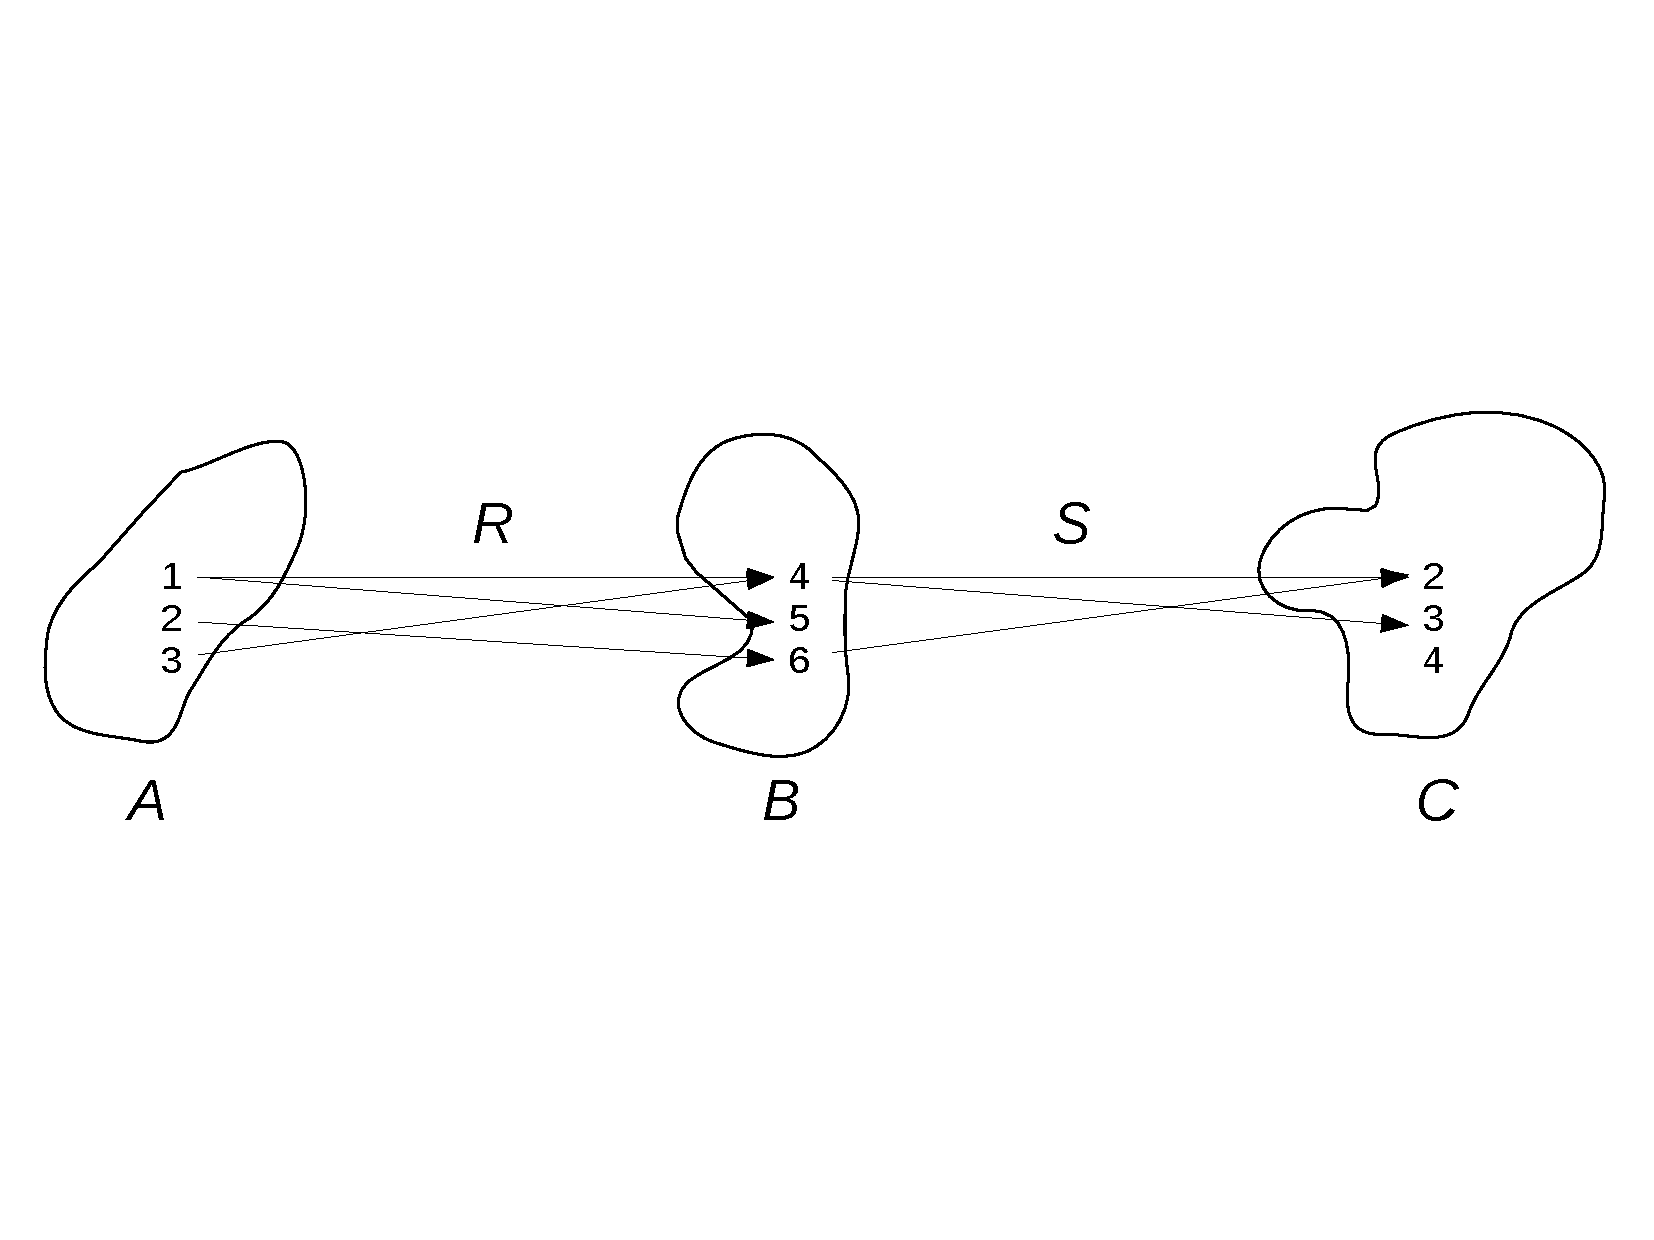
\includegraphics[width=15cm,trim={0.5cm 7cm 0.5cm 6.8cm},clip]{./figuras/figure21.pdf}
\end{center}
\end{figure}

Alguns c\'alculos revelam: 
\begin{enumerate}[{\bf a)}]
\item $S\bola R=\{(1,2),(1,3),(3,2),(3,3),(2,2)\}$.
\item $R^{-1}=\{(4,1),(5,1),(6,2),(4,3)\}$.
\item $S^{-1}=\{(2,4),(3,4),(2,6)\}$.
\item $R^{-1}\bola S^{-1}=\{(2,1),(3,1),(2,3),(2,2),(3,3)\}$.
\item $(S\bola R)^{-1}=\{(2,1),(3,1),(2,3),(3,3),(2,2)\}$.
\end{enumerate}
Note que, $R\bola S$ e $S^{-1}\bola R^{-1}$ n\ao est\ao definidos e que $R^{-1}\bola S^{-1}=(S\bola R)^{-1}$.

Para um pouco mais de pr\'atrica em demonstra\cao de teoremas vamos mostrar que esta ultima igualdade sempre vale:
\begin{teob}
Sejam $A,B,C$ conjuntos, $R$ uma rela\cao de $A$ em $B$ e $S$ uma rela\cao de $B$ em $C$. Ent\ao $(S\bola R)^{-1}=R^{-1}\bola S^{-1}$.
\end{teob}
\begin{proof}
Para esta demonstra\caoi, considere a figura abaixo para manter em mente os v\'arios conjuntos e rela\coes involvidas.
\begin{figure}[h]
\begin{center}
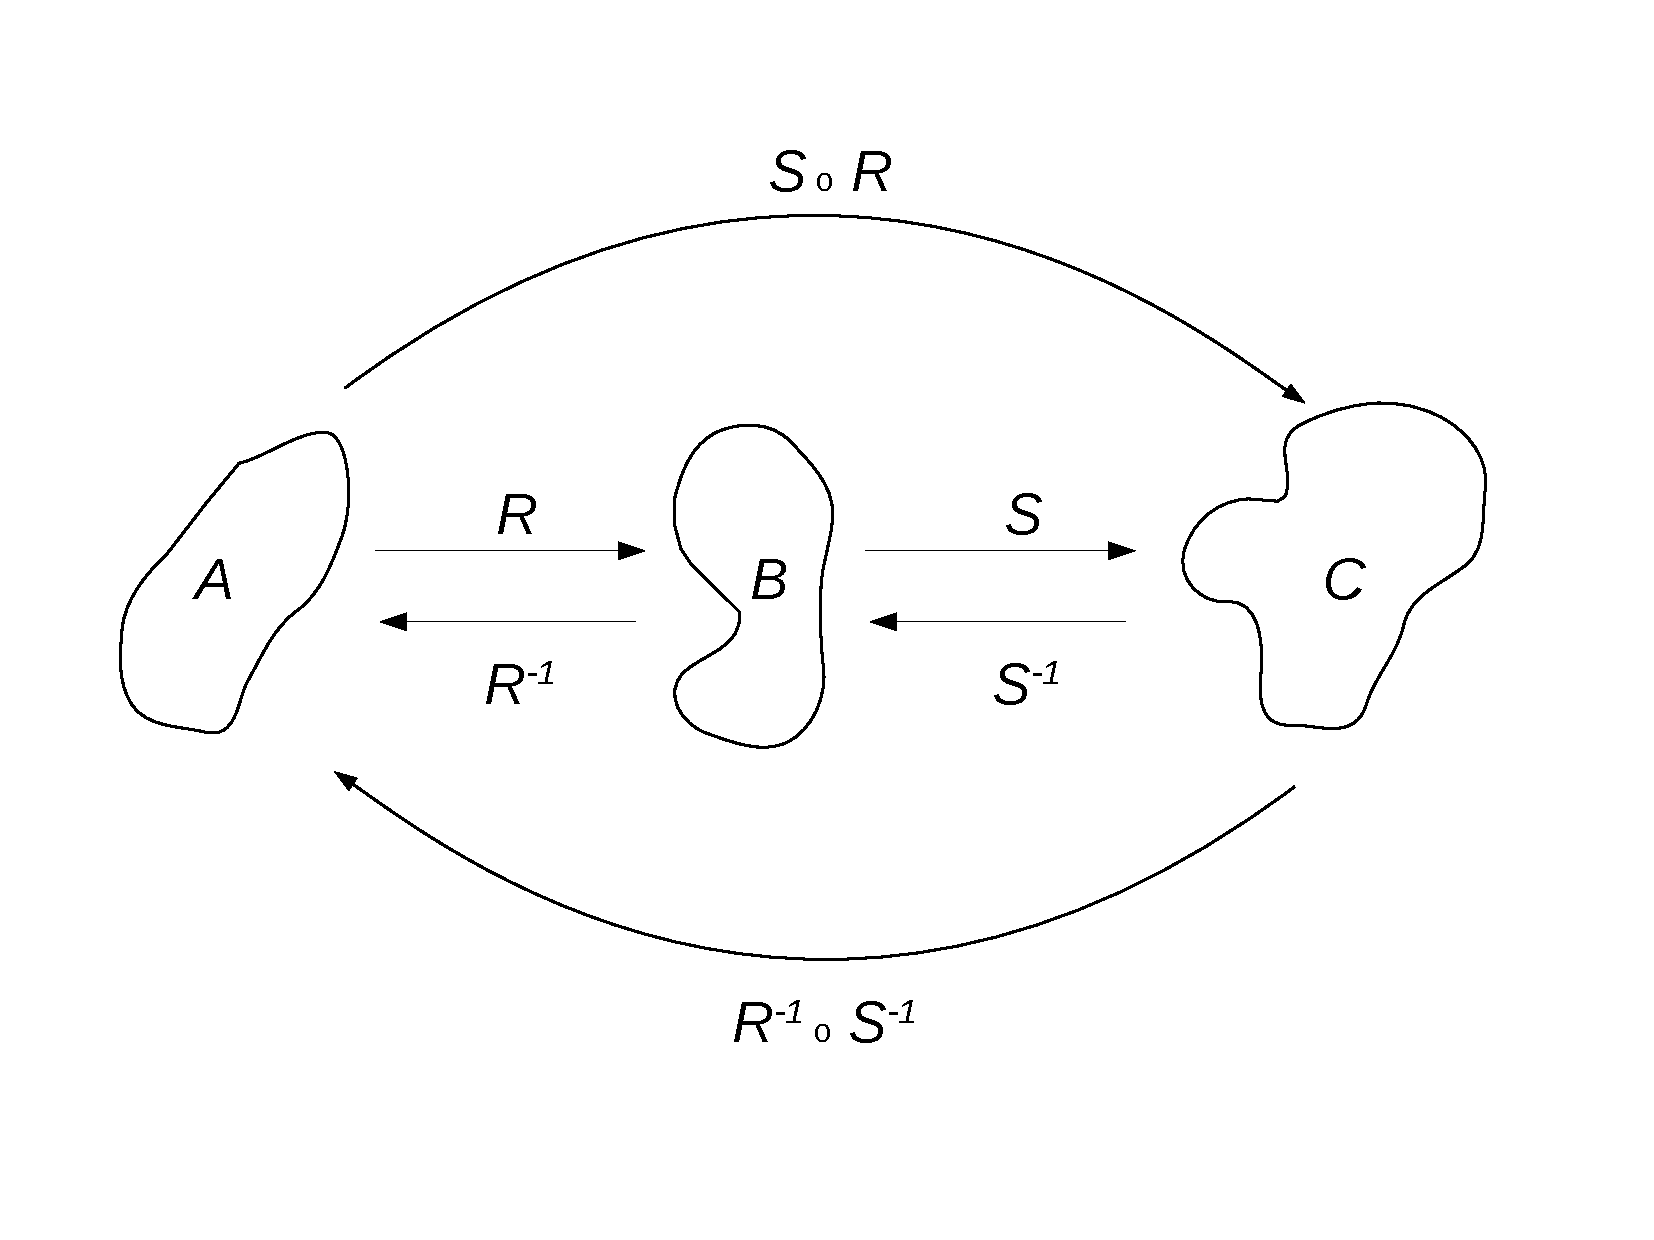
\includegraphics[width=13cm,trim={2cm 2.5cm 2cm 2.5cm},clip]{./figuras/figure22.pdf}
\end{center}
\end{figure}
Primeiro, observe que $(S\bola R)^{-1}$ \'e uma rela\cao de $C$ em $A$ assim como $(S\bola R)^{-1}$, isso diz que estas rela\coes t\^em a chance de serem iguais. Lembrando que rela\coes s\ao conjuntos, portanto para mostrar que duas rela\coes s\ao iguais, devemos mostrar que elas s\ao iguais como conjuntos. Para come\cc ar, seja $(x,z)\in (S\bola R)^{-1}$. Ent\ao $(z,x)\in S\bola R$, logo existe um $y\in B$ tal que $(z,y)\in R$ e $(y,x)\in S$. Consequentemente, $(y,z)\in R^{-1}$ e $(x,y)\in S^{-1}$. Portanto, $(x,z)\in R^{-1}\bola S^{-1}$, assim $(S\bola R)^{-1}\subseteq R^{-1}\bola S^{-1}$.

Agora para mostrar a outra inclus\ao, seja $(x,z)\in R^{-1}\bola S^{-1}$. Ent\ao existem um $y\in B$, tal que $(x,y)\in S^{-1}$ e $(y,z)\in R^{-1}$. Consequentemente, $(y,z)\in S$ e $(z,y)\in R$, portanto temos $(z,x)\in S\bola R$, logo $(x,z)\in (S\bola R)^{-1}$ como desejado.
\end{proof}
\\

Embora a demonstra\cao anterior possa parecer um pouco complicado, mas cada passo apenas envolveu tradu\cao para linguagem de conjuntos uando as defini\cois, por exemplo $(x,y)\in S^{-1}$ significa que $(y,x)\in S$. Em outras palavras, este resultado nos diz que a inversa de uma composi\cao de rela\coes \'e acomposi\cao das inversas na ordem oposta.

Agora apresentamos um exemplo envolvendo composi\caoi. Seja $A=\{1,2,3\}$, $B=\{4,5,6\}$, $C=\{6,7,8\}$ e $D=\{1,4,6\}$ com
\begin{equation*}
 \begin{aligned}
R=&\espaco\{(1,4),(3,5),(3,6)\} \textrm{ uma rela\cao de $A$ em $B$},\\
S=&\espaco\{(4,6),(6,8)\} \textrm{ uma rela\cao de $B$ em $C$},\\
T=&\espaco\{(6,1),(8,6),(6,4)\} \textrm{ uma rela\cao de $C$ em $D$}.
 \end{aligned}
\end{equation*} 
Estas rela\coes est\ao ilustradas na figura abaixo:
\begin{figure}[h]
\begin{center}
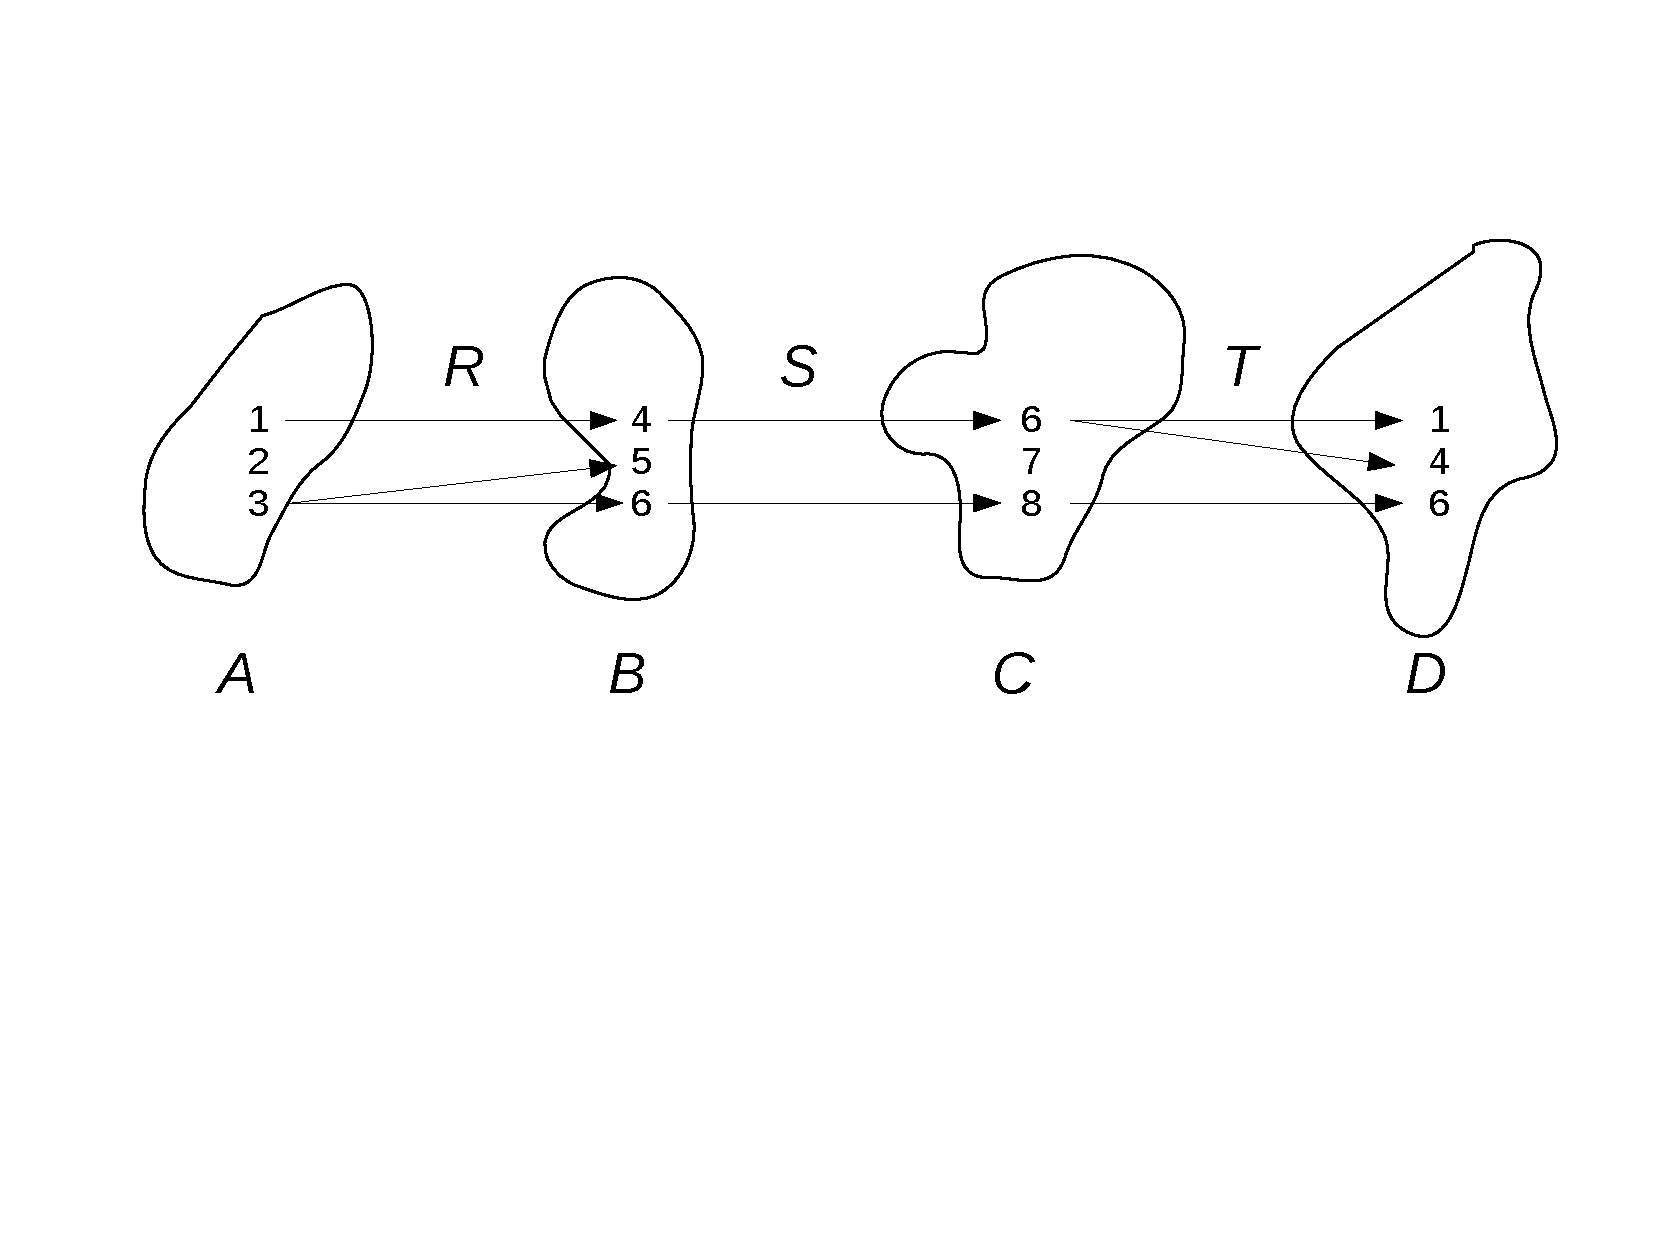
\includegraphics[width=15cm,trim={1.5cm 10cm 1.5cm 4cm},clip]{./figuras/figure23.pdf}
\end{center}
\end{figure}

Ent\ao podemos formar
\begin{equation*}
 \begin{aligned}
S\bola R=&\espaco\{(1,6),(3,8)\} \textrm{ uma rela\cao de $A$ em $C$},\\
T\bola S=&\espaco\{(4,1),(4,4),(6,6)\} \textrm{ uma rela\cao de $B$ em $D$}.
 \end{aligned}
\end{equation*}
Agora, estas podem ser compostas com $T$ e $R$ para obter:
\begin{equation*}
 \begin{aligned}
T\bola(S\bola R)=&\espaco\{(1,1),(1,4),(3,6)\} \textrm{ uma rela\cao de $A$ em $C$},\\
(T\bola S)\bola R=&\espaco\{(1,1),(1,4),(3,6)\} \textrm{ uma rela\cao de $B$ em $D$}.
 \end{aligned}
\end{equation*}

Incrivelmente, estas duas igualdades s\ao iguais! N\ao somos excepcionalmente sortudos em nossas escolhas de $R$, $S$ e $T$. Entretanto, esta igualdade \'e sempre v\'alida. Matem\'aticos expressam isto dizendo ``a composi\cao de rela\coes \'e associativa.''\index{Rela\caoi!Associatividade} Agora apresentamos a demonstra\cao disso:
\begin{teob}\label{relto1}
Sejam $A,B,C$ e $D$ conjuntos com $R$ uma rela\cao de $A$ em $B$, $S$ uma rela\cao de $B$ em $C$ e $T$ uma rela\cao de $C$ em $D$. Ent\ao
\[
T\bola(S\bola R)=(T\bola S)\bola R.
\]
\end{teob}
\begin{proof}
A figura abaixo nos ajudar\'a a ver as v\'arias rela\coes envolvidas:
\begin{figure}[h]
\begin{center}
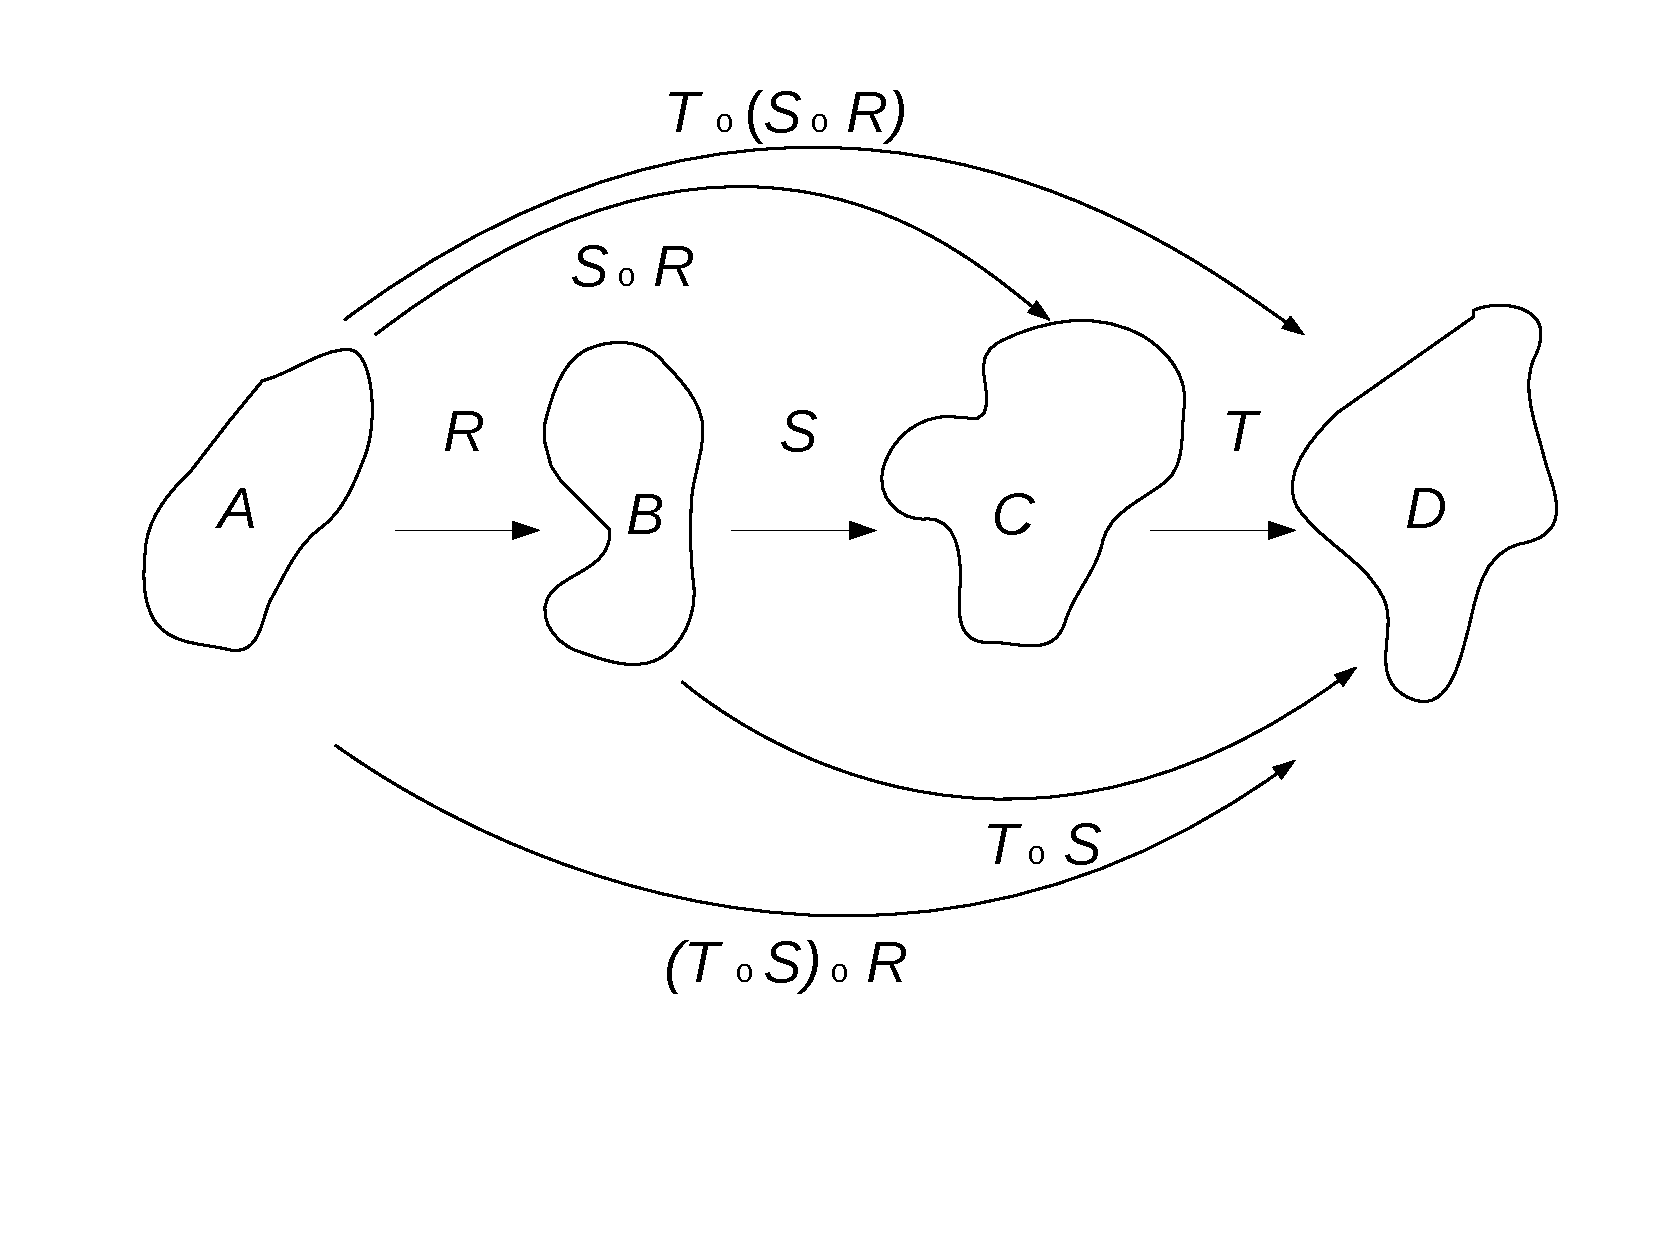
\includegraphics[width=13cm,trim={1cm 1.5cm 1cm 1.5cm},clip]{./figuras/figure24.pdf}
\end{center}
\end{figure}

Precisamos mostras a inclus\ao de conjuntos em ambos os lados. Primeiro, para ver que $T\bola(S\bola R)\subseteq(T\bola S)\bola R$, seja $(x,y)\in T\bola(S\bola R)$. En\tao $x\in A$ e $y\in D$ e exsite $z\in C$ tal que $(x,z)\in S\bola R$ e $(z,y)\in T$. Como, $(x,z)\in S\bola R$, existe $w\in B$ tal que $(x,w) \in R$ e $(w,z)\in S$. Agora, $(w,z)\in S$ e $(z,y)\in T$ implicam que $(w,y)\in T\bola S$. Mas $(x,w) \in R$, assim $(x,y)\in (T\bola S)\bola R$. A demonstra\cao de que a outra inclus\ao \'e v\'alida fica como excerc\ih cio.
\end{proof}
\\

Podemos tambem combinar algumas das propriedades especiais de rela\coes com estas opera\cois. Por exemplo, temos:
\begin{teob}
Seja $R$ uma rela\cao em $A$. Ent\ao $R$ \'e transitiva se e somente se $R\bola R\subseteq R$
\end{teob}
\begin{proof}
Como este teorema \'e uma equival\^encia, temos que demostrar duas implica\cois. Come\cc aremos mostrando que $R$ transitiva implica $R\bola R\subseteq R$. Seja $(x,y)\in R\bola R$. Ent\ao existe $z\in A$ tal que $(x,z)\in R$ e $(z,y)\in R$. Mas, como $R$ \'e transitiva temos que $(x,y)\in R$. Portanto, $R\bola R\subseteq R$.

Agora, mostremos que $R\bola R\subseteq R$ implica que $R$ seja transitiva. Suponha que $(x,y)$ e $(y,z)$ sejam elementos de $R$. Ent\aoi, $(x,z)\in R\bola R$ e como $R\bola R\subseteq R$, $(x,z)$ deve necessariamente ser um elemento de $R$ e assim, $R$ \'e transitiva. 
\end{proof}
\\

N\ao podemos abster-nos de notar mais uma vez qua a forma de demonstra\cao aqui foi determinada pela conclus\ao de cada implica\caoi. Para a primeira, a conclus\ao era $R\bola R\subseteq R$, postanto usamos a t\'ecnica usual de subconjunto para come\cc ar com elemento fixo mas arbitr\'ario em um conjunto e mostrando que este era um elemento do outro conjunto. Na segunda implica\cao, a conclus\ao era que $R$ seria transitiva, neste caso, mostramos que $R$ stisfazia a defini\cao de transitividade. Em ambos os casos as hip\'oteses vieram durante a demonstra\cao e n\ao no come\cc o.

\paragraph{Excerc\ih cios \ref{mrelacoes}}

\begin{enumerate}[{\bf 1.}]

%excercicio1
\item Sejam $A=\{1,2,4\}$ e $B=\{1,3,4\}$. Sejam $R=\{(1,3),(1,4),(4,4)\}$ uma rela\cao de $A$ em $B$, $S=\{(1,1),(3,4),(3,2)\}$ uma rela\cao de $B$ em $A$ e $T=\varnothing$ uma rela\cao de $A$ em $B$. Encontre:
\begin{enumerate}[a)]
\item $\Dom(R)$.
\item $\Dom(S)$.
\item $\Dom(T)$.
\item $\Ima(R)$.
\item $\Ima(S)$.
\item $\Ima(T)$.
\item $S\circ R$.
\item $R\circ S$.
\item $\Dom(S\circ R)$.
\item $\Ima(S\circ R)$.
\item $\Dom(R\circ S)$.
\item $\Ima(R\circ S)$.
\item $R^{-1}$.
\item $S^{-1}$.
\item $I_A$.
\item $I_B$.
\item $R^{-1}\circ S^{-1}$.
\item $S^{-1}\circ R^{-1}$.
\item $(R\circ S)^{-1}$.
\item $(S\circ R)^{-1}$.
\item $T^{-1}$.
\item $I_B^{-1}$.
\item $(R\bola S)\bola R$.
\item $R\bola(S\bola R)$. 
\end{enumerate}

%excercicio2
\item Seja $R$ uma rela\cao em um conjunto n\ao vazio $A$. Mostre que:
\begin{enumerate}[a)]
\item $(R^{-1})^{-1}=R$
\item $I_A^{-1}-I_A$
\item $R$ \'e reflexiva se e somente se $I_A\subseteq R\subseteq R\bola R$.
\item $R$ \'e sim\'etrica se e somente se $R=R^{-1}$.
\item $R$ \'e transitiva se e somente se $R^{-1}$ \'e transitiva.
\item $R$ \'e uma rela\cao de equival\^encia e se somente se $R^{-1}$ \'e uma rela\cao de equival\^encia.
\item Suponha que $\Dom(R)=A$. $R$ \'e uma rela\cao de equival\^encia se e somente se $R=R^{-1}=R\bola R$.
\item $R$ \'a assim\'etrica se e somente se $R\inter R^{-1}=\varnothing$.
\item $R\uni R^{-1}=A\times A$ implica que $R$ \'e completa.
\item $R$ sim\'etrica implica $R\bola R$ \'e sim\'etrica.
\item $I_{\Dom(R)}\subseteq R^{-1}\bola R$.
\item $R$ \'e uma ordem parcial se e somente se $R^{-1}$ \'e uma ordem parcial.
\item $R$ \'e uma ordem parcial se e somente se $R\inter R^{-1}=I_A$ e $R\bola R=R$.
\item $R$ \'e uma ordem parcial estrita se e somente se $R^{-1}$ \'e uma ordem parcial estrita.
\end{enumerate}

%excercicio3
\item Seja $A$ um conjunto n\ao vazio com $R,S$ rela\coes em $A$. Considere as seguintes conjecturas. Prove as verdadeiras e d\^e exemplos para aquelas que s\ao falsas.
\begin{enumerate}[a)]
\item $R$ \'e sim\'etrica implica $R\bola R$ sim\'etrica.
\item $R\bola S^{-1}=S\bola R^{-1}$ implica que $R\bola S^{-1}$ seja sim\'etrica.
\end{enumerate}

%excercicio4
\item Seja $R$ uma rela\cao de $A$ em $B$ e $S$ uma rela\cao  de $B$ em $C$. Mostre que:
\begin{enumerate}[a)]
\item $\Dom(S\bola R)\subseteq \Dom(R)$.
\item $\Ima(S\bola R)\subseteq \Ima(S)$.
\item $\Ima(R)\subseteq \Dom(S)$ implica $\Dom(S\bola R)=\Dom(R)$. A rec\ih proca \'e verdadeira? 
\end{enumerate}

%excercicio5
\item Complete a demonstra\cao do teorema \ref{relto1}.

%excercicio6
\item Suponha que $R$ e $S$ sejam rela\coes de equival\^encia em um conjunto n\ao vazio $A$. Considere as seguintes conjecturas. Prove as verdadeiras e d\^e exemplos para aquelas que s\ao falsas. 
\begin{enumerate}[a)]
\item $R\uni S$ \'e uma rela\cao de equival\^encia implica que $R\bola S=S\bola R$.
\item $R\uni S= R\bola S$ implica que $R\uni S$ \'e uma rela\cao de equival\^encia.
\item $R\uni S= R\bola S$ implica que $R\bola S=S\bola R$.
\end{enumerate}

%excercicio7
\item Seja $R$ a rela\cao $<$ nos inteiros. Mostre que $R$ \'e uma ordem parcial estrita. Tamb\'em mostre que $R\uni I_{\mathbb{Z}}$ (que \'e $\leq$) \'e uma ordem parcial.

%excercicio8
\item Seja $R$ uma ordem parcial em um conjunto n\ao vazio $A$. Mostre que $R-I_A$ \'e uma ordem parcial estrita em $A$.

%excercicio9
\item Seja $R$ uma rela\cao em um conjunto n\ao vazio $A$. Prove ou d\^e contraexemplos (refira-se ao excerc\ih cio \ref{relexer17}, da se\cao \ref{relacoes}):
\begin{enumerate}[a)]
\item $R_{ref}=R\uni I_A$. 
\item $R_{sim}=R\uni R^{-1}$.
\item $R_{trans}=R\uni (R\bola R)$.
\end{enumerate}

%excercicio10
\item Sejam $R,S$ e $T$ rela\coes entre conjuntos. Determine algumas condi\coes sobre $R,S$ e $T$ para garantir as seguintes conclus\ois. Demonstre que suas conjecturas est\ao corretas.
\begin{enumerate}[a)]
\item $R\bola S=R\bola T$ implica $S=T$.
\item $S\bola R=T\bola R$ implica $S=T$.
\end{enumerate}

%excercicio11
\item {\bf Acredite se quiser:}  

\noindent \textit{\textbf{Conjectura:}} Seja $R$ uma rela\cao em um conjunto n\ao vazio $A$. Se $R$ \'e transitiva ent\ao $R\bola R$ \'e transitiva.

\noindent \textit{\textbf{``Demonstra\caoi'':}} Seja $R$ uma rela\cao transitiva em $A$. Sejam $a,b,c\in A$ com $(a,b),(b,c)\in R\bola R$. Ent\ao existem $d,e\in A$ tais que $(a,d),(d,b),(b,e),(e,c)\in R$. Como $R$ \'e transitiva $(a,b),(b,c)\in R$, isso implica que $(a,c)\in R\bola R$, logo $R\bola R$ \'e transitiva.

\noindent \textit{\textbf{``Contraexemplo'':}} Seja, $A=\{1,2,3\}$ $R=\{(1,2),(2,2),(2,3),(1,3)\}$. Assim,
\[
R\bola R=\{(1,3),(1,2),(2,3),(2,2)\},
\]
logo temos $R$ transitiva e $R\bola R$ n\aoi.

%excercicio12
\item {\bf Acredite se quiser:}  

\noindent \textit{\textbf{Conjectura:}} Sejam $R,S$ rela\coes de equival\^encia em um conjunto n\ao vazio $A$. Se $R\bola S=S\bola R$ ent\ao $R\uni S$ \'e uma rela\cao de equival\^encia.

\noindent \textit{\textbf{``Demonstra\caoi'':}} Sejam $R,S$ como acima. Claramente, $R\uni S$ \'e reflefiva. Se $(a,b)\in R\uni S$ ent\ao $(a,b)\in R$ ou $(a,b)\in S$. Se $(a,b)\in R$, e como $R$ \'e sim\'etrica, $(b,a)\in R$, logo $(b,a)\in R\uni S$. Por argumentos semelhantes, se $(a,b)\in S$ ent\ao $(b,a)\in S$, isto demonstra que $R\uni S$ \'e sim\'trica. Aogra, sejam $(a,b),(b,c)\in R\uni S$. Se ambos pertencem a $R$, ou se ambos pertencem a $S$, a transitividade de cada um implica que $R\uni S$ \'e transitiva. Portanto, suponha que $(a,b)\in R$ e $(b,c)\in S$. Como $R\bola S=S\bola R$ e $(a,c)\in S\bola R$, $(a,c)\in R\bola S$. Assim existe $d\in A$ tal que $(a,d)\in S$ e $(d,c)\in R$. Mas, ambos $R$ e $S$ s\ao sim\'etricos, portanto $(c,d)\in R$ e $(d,a)\in S$. Logo, $(c,a)\in R$. Mas $R$ \'e sim\'etrica, assim temos $(a,c)\in R$ e consequentemente $R\uni S$ \'e transitiva. Argumentos similares podem ser utilizados no caso $(a,b)\in S$ e $(b,c)\in R$.

\noindent \textit{\textbf{``Contraexemplo'':}} Sejam 
\begin{equation*}
 \begin{aligned}
A=&\{a,b,c,d\},\\
R=&I_A\uni\{(a,b),(b,a),(a,c),(c,a)\},\\
S=&I_A\uni\{(c,d),(d,c),(a,c),(c,a),(d,a),(a,d)\}.
 \end{aligned}
\end{equation*}
Ent\ao $R,S$ s\ao rela\coes de equival\^encia com $R\bola S=S\bola R$, mas $R\uni S$ cont\'em $(b,a)$ e $(a,d)$ mas n\ao $(b,d)$ e assim n\ao \'e transitiva.

%excercicio13
\item {\bf Acredite se quiser:}  

\noindent \textit{\textbf{Conjectura:}} Seja $R$ uma ordem total estrita em um conjunto n\ao vazio $A$. Ent\ao $S=(A\times A)-R$ \'e uma ordem total em $A$. 

\noindent \textit{\textbf{``Demonstra\caoi'':}} Como $R$ \'e irreflexiva, $I_A\inter R=\varnothing$ portanto $I_A\subseteq S$ e $S$ \'e reflexiva. Agora suponha que $(a,b),(b,c)\in S$. $R$ \'e completa, assim como $(a,b),(b,c)\in S$, temos que $(b,a),(c,b)\in R$. A trnasitividade de $R$ implica que $(c,a)\in R$. Se $(a,c)\in R$ ent\ao $(a,a)\in R$, que \'e imposs\ih vel, consequentemente $(a,c)\in S$ e $S$ \'e transitiva. Agora, suponha que $(a,b),(b,a)\in S$. Ent\ao devemos ter $a=b$, caso contr\'ario $R$ n\ao seria completa. Assim $S$ \'e uma ordem parcial. Se $a,b\in A$, $a\neq b$ e $(a,b)\notin S$, ent\ao $(a,b)\in R$, e como notado anteriormente, isto implica $(b,a)\in S$ e consequentemente $S$ \'e completa e assim uma ordem total.

\noindent \textit{\textbf{``Contraexemplo'':}} Sejam $A=\{1,2,3\}$ e $R=\{(1,2),(2,3),(3,1)\}$. Ent\ao
\[
S=\{(1,1),(2,2),(3,3),(2,1),(1,3),(3,2)\}
\]
n\ao \'e uma ordem total pois n\ao \'e transitiva ($(1,3),(3,2)\in S$, mas $(1,2)\notin S$).
\end{enumerate}
%%%%%%%%%%%%%%%%%%%%%%%%%%%%%%%%%%%%%%%%%%%%%%%%%%%%%%%%%%%%%%%%%%%%%%%%%%%%%%%%%%%%%%%%%%%%

\section{Rela\coes de Equival\^encia e Parti\cois}\label{equivalencia}

Vamos dar uma olhada mais de perto nas rela\coes de equival\^encia $R$ que estavam no exemplo \ref{relex11} da se\cao \ref{relacoes} (lembremos que $R$ era uma rela\cao em $\mathbb{N}$ dada por $xRy$ se e somente se $5|(x-y)$). Se definirmos $S_i=\{x: xRi\}$, vemos que:
\begin{equation*}
 \begin{aligned}
S_1&=\{x: xR1\}=\{1,6,11,16,\ldots\},\\
S_2&=\{x: xR2\}=\{2,7,12,17,\ldots\},\\
S_3&=\{x: xR3\}=\{3,8,13,18,\ldots\},\\
S_4&=\{x: xR4\}=\{4,9,14,19,\ldots\},\\
S_5&=\{x: xR5\}=\{5,10,15,20,\ldots\},\\
S_6&=\{x: xR6\}=\{1,6,11,16,\ldots\}=S_1,\\
S_7&=S_2,\\
S_8&=S_3,\\
& \vdots\\
 \end{aligned}
\end{equation*}
ou melhor graficamente:

\begin{figure}[h]
\begin{center}
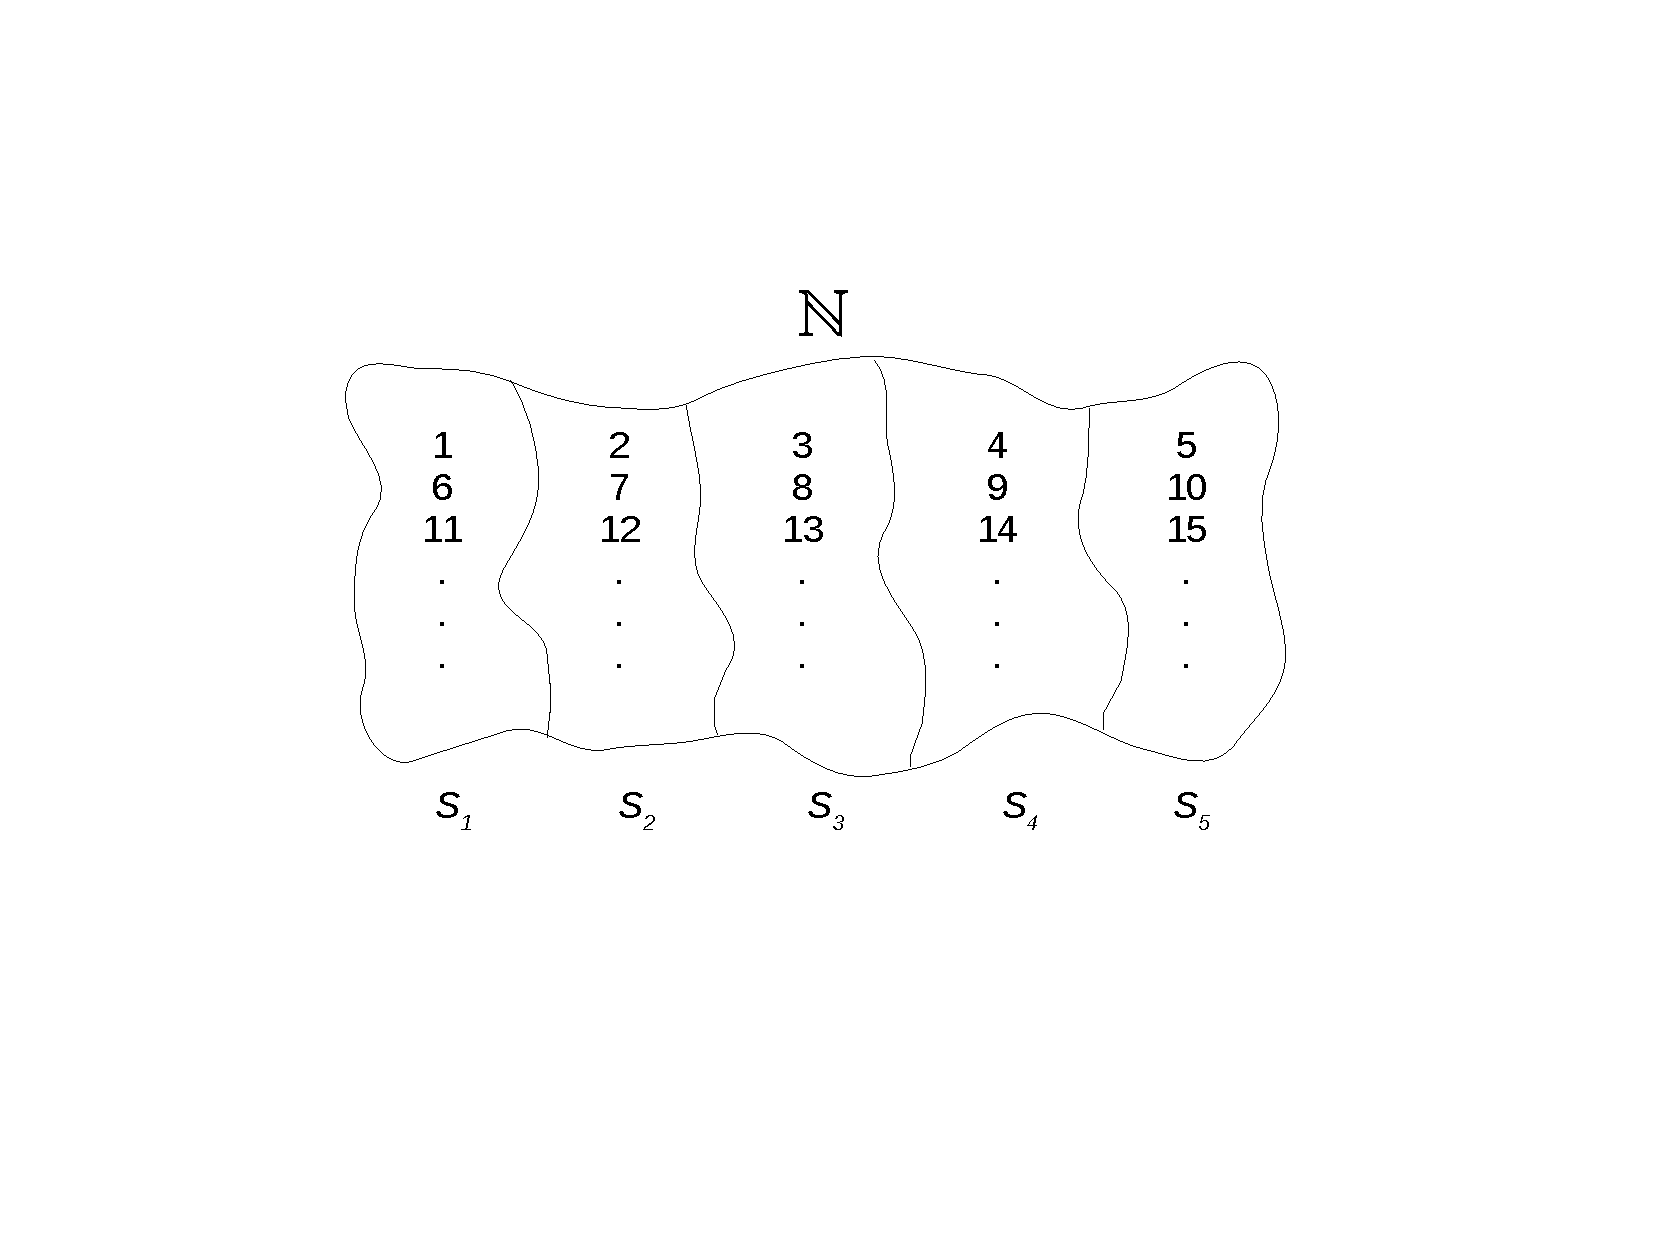
\includegraphics[width=13cm,trim={3cm 6.5cm 3cm 4cm},clip]{./figuras/figure25.pdf}
\end{center}
\end{figure}

Existem muitas coisas interessantes sobre estes conjunto para serem notadas. Enquanto em um primeiro momento algu\'em poderia supor que existe um n\'umero infinito deles, mas existem apenas cinco. Tamb\'em, a uni\ao destes cinco conjuntos \'e todo o $\mathbb{N}$, isto \'e dado um elemento $y\in\mathbb{N}$, $y$ \'e um elemento de um destes cinco conjuntos. Para ser mais preciso, existe exatamente um destes conjuntos que tem $y$ como elemento. Isto significa (ceja exemplo \ref{eqexe2} abaixo) que, dados quaisquer dois destes conjuntos, ou eles s\ao iguais, ou eles s\ao disjuntos. Veremos em breve que toda rela\cao de equival\^encia gera conjuntos com essas propriedades, mas primeiro precisamos de algumas defini\cois. 
\begin{definb}
Seja $A$ um conjunto n\ao vazio. Uma {\it parti\cao}\index{Parti\caoi} $\Pi$ de $A$ \'e uma cole\cao de subconjuntos n\ao vazios de $A$ tais que cada elemento de $A$ \'e elemento de exatamente um destes conjuntos.
\end{definb}

Note que se $\Pi$ \'e uma parti\cao de $A$, en\tao os elementos de $\Pi$ s\ao subconjuntos de $A$, chamamaremos eles de os {\it blocos}\index{Parti\caoi!Blocos} de $\Pi$. Vemos ent\aoi, devido a defini\caoi, que se $B$ e $C$ s\ao blocos de $\Pi$, ent\ao ou $B=C$ ou $B\inter C=\varnothing$. Tamb\'em, a uni\ao de todos os elementos de $\Pi$ \'e $A$. Assim, podemos pensar que uma parti\cao de um conjunto como uma separa\cao do conjunto em partes disjuntas, por exemplo, podemos considerar as tr\^es classes de ensino (fundamental, m\'edio e superior) como uma parti\cao do corpo de estudantes. Agora apresentamos alguns exemplos de parti\cois:

\paragraph{{\bf Exemplos}}
\begin{enumerate}[{\bf 1.}]
\item\label{eqexe1} Seja $A$ n\ao vazio. En\tao $\Pi_1=\{\{x\}:x\in A\}$ e $\Pi_2=\{A\}$ s\ao parti\coes de $A$. Em certo senso, $\Pi_1$ \'e aparti\cao mais ``fina'' de $A$ equanto $\Pi_2$ \'e a mais grossa (veja o exerc\ih cio \ref{eqrexcerc3} desta se\caoi).
\item\label{eqexe2} Seja $A=\{1,2,3,4\}$. En\tao $\Pi_1=\{\{1\},\{2,3\},\{4\}\}$ e $\Pi_2=\{\{1,4\},\{2,3\}\}$ s\ao parti\cois de $A$.
\item\label{eqexe3} Referindo-se aos conjuntos $S_i$ mencionados no come\cc o desta se\caoi, vemos que $\{S_1,S_2,S_3,S_4,S_5\}$ \'e uma parti\cao de $\mathbb{N}$.
\end{enumerate}

Exsite uma rela\cao pr\'oxima entre parti\coes e classes de equival\^encia, de fato, dada uma rela\cao de equival\^envia em um conjunto podemos gerar uma parti\caoi (como fizemos com $\mathbb{N}$ acima) e dada uma parti\cao podemos gerar uma rela\cao de equival\^encia. Para ver como isto realmente funciona, precisamos de mais uma defini\caoi:
\begin{definb}
Seja $R$ uma rela\cao de equival\^encia em um conjunto n\ao vazio $A$. Seja $x\in A$. A {\it classe de equival\^encia}\index{Classe de Equiva\^encia} de $x$ m\'odulo $R$, denotada por $[x]_R$ (ou \`as vezes $x/R$), \'e o conjunto de todos os elementos de $A$ que s\ao R-relacionados a $x$. Em s\ih mbolos,
\[
[x]_R=\{y\in A: yRx\}.
\]
O conjunto de tais classes de equival\^encia \'e denotado por $[A]_R$ (ou \`as vezes A/R) e \'e chamado $A$ m\'odulo R. Em s\ih mbolos,
\[
[A]_R=\{[x]_R: x\in A\}.
\]
\end{definb}
Referindo-se mais uma vez ao exemplo do come\cc o da se\caoi, temos:
\begin{equation*}
 \begin{aligned}
{[2]}_R=&\espaco S_2 = \{2,7,12,17,\ldots\},\\
[4]_R=&\espaco [9]_R = [14]_R,\\
[\mathbb{N}]_R=&\espaco \{[1]_R,[2]_R,[3]_R,[4]_R,[5]_R\} = \{[6]_R,[12]_R,[18]_R,[9]_R,[25]_R\}.
 \end{aligned}
\end{equation*}
Para dois exemplos extremos, seja $A$ um conjunto n\ao vazio e seja $R$ a igualdade (isto \'e, $xRy$ se e somente se $x=y$) e seja $S=A\times A$ (tamb\'em uma rela\cao de equival\^encia). En\tao
\begin{equation*}
 \begin{aligned}
&\forall x\in A, [x]_R=\{x\} \textrm { e } [x]_S=A,\\
&[A]_R=\{\{x\}:x\in A\},\\
&[A]_S=\{A\}.
 \end{aligned}
\end{equation*}
No caso de $R$ temos cada classe de equival\^encia contendo exatamente um elemento enquanto que no caso de $S$ existe apenas uma grande classe de equivl\^encia consistindo de todo o conjunto $A$.

Talvez por agora o leitor pensou que $[A]_R$ \'e uma parti\cao de $A$, com as classes de quival\^encia formando os blocos da parti\caoi. Isto \'e, de fato, o caso que demonstraremos em breve, mas antes vamos estabelecer algumas propriedades das classes de equival\^encia.
\begin{teob}\label{relteo1}
Seja $R$ uma rela\cao de equival\^encia em um conjunto n\ao vazio $A$. En\tao
\begin{enumerate}[{\bf a)}]
\item $\forall x\in A, [x]_R\neq\varnothing$.
\item $\forall x,y\in A, [x]_R\inter[y]_R\neq\varnothing$ se e somente se $xRy$.
\item $\forall x,y\in A,[x]_R=[y]_R$ se e somente se $xRy$.
\item $\forall x,y\in A, [x]_R\neq[y]_R$ se e somente se $[x]_R\inter[y]_R=\varnothing.$
\end{enumerate}
\end{teob}
\begin{proof}
 \begin{enumerate}[{\bf a)}]
\item Como $R$ \'e reflexiva, $xRx$ para todo $x\in A$, logo $x\in[x]_R$ e assim $\forall x\in A, [x]_R\neq\varnothing$.
\item Suponha que $z\in [x]_R\inter [y]_R$. Ent\ao $xRz$ e $yRz$. Como $R$ \'e sim\'etrica, $zRy$ e como $R$ \'e tamb\'em transitiva, temos $xRy$ como desejado. Agora, suponha que $xRy$. Ent\ao $y\in[x]_R$. Mas $y\in[y]_R$ tamb\'em, portanto, $[x]_R\inter[y]_R\neq\varnothing$. 
\item Se $[x]_R=[y]_R$ entao $y\in[x]_R$, logo $xRy$. Agora suponha $xRy$ e seja $z\in[x]_R$. Ent\ao $xRz$. Pela simetria de $R$ temos que $yRx$ e pela transitividade de $R$ obtemos $yRz$, logo $z\in[y]_R$ e consequentemente, $[x]_R\subseteq[y]_R$. Um argumento similar (apenas trocar os papeis de $x$ e $y$) mostra que $[y]_R\subseteq[x]_R$, que completa a demonstra\caoi.
\item Segue diretamente dos partes b) e c).
\end{enumerate}
\end{proof}
\\

Terminamos a maior parte do trabalho para mostrar que $[A]_R$ \'e uma parti\caoi de $A$, o que resta est\'a na demonstra\cao do teorema abaixo.
\begin{teob}
Sejam $A$ um conjunto n\ao vazio e $R$ uma rela\cao de equival\^encia em $A$. Ent\ao $[A]_R$ \'e uma parti\cao de $A$.
\end{teob}
\begin{proof}
Devemos mostrar que $[A]_R$ \'e uma cole\cao de subconjuntos n\ao vazios de $A$ que tem a propriedade que cada $x\in A$ \'e um elemento de exatamente uma dos conjuntos de $[A]_R$. Como $[A]_R=\{[x]_R: x\in A\}$ e $x\in[x]_R$ para casa $x\in A$, cada membro de $[A]_R$ \'e n\ao vazio. Isto tamb\'em mostra que cada $x\in A$ \'e um elemento de pelo menos um conjunto, chamado sua pr\'opria classe de equival\^encia. Suponha que existe $y\in A$ tal que $y$ \'e um elemento de dois conjuntos de $[A]_R$. Mas, o teorema anterior \ref{relteo1} mostrou que distintos elementos de $[A]_R$ s\ao disjuntos, o que contradiz o fato de $y$ pertencer a ambas classes de equival\^encia. Portanto, cada elemento de $A$ \'e um elemento de exatamente uma das classes de equival\^encia.
\end{proof}
\\

Assim, vemoa que uma rela\cao de equival\^encia em um conjunto induz uma parti\cao deste conjunto. Este processo tamb\'em funciona a rec\ih proca, isto \'e uma parti\cao de um conjunto induz uma rela\cao de equival\^encia no conjunto. Antes de mostrar este fato precisamos dar um nome para tal rela\caoi. 
\begin{definb}
Seja $\Pi$ uma parti\cao de um conjunto $A$. Definimos a rela\cao $A/\Pi$ (l\^e-se ``$A$ m\'odulo $\Pi$'') em $A$ por $(x,y)\in A/\Pi$ se e somente se existe $B\in\Pi$ tal que $\{x,y\}\subseteq B$. Em palavras, $x$ \'e relacionado a $y$ se e somente se $x$ e $y$ s\ao ambos elementos do mesmo bloco da parti\caoi.
\end{definb}

Referindo-se a $\Pi_2$ do exemplo \ref{eqexe2} dado anteriormente nesta se\caoi, temos
\[
A/\Pi_2=\{(1,1),(1,4),(2,2),(2,3),(3,2),(3,3),(4,1),(4,4)\}.
\]
Uma r\'apida olhada revela que $A/\Pi$ \'e uma rela\cao de equival\^encia, embora, claramente, devemos provar que isto \'e sempre o caso.
\begin{teob}
Seja $\Pi$ uma parti\cao de um conjunto n\ao vazio $A$. Ent\ao $A/\Pi$ \'e uma rela\cao de equival\^encia em $A$.
\end{teob}
\begin{proof}
Seja $\Pi$ uma parti\cao de $A$ e para conveni\^encia de nota\cao vamos escrever $A/\Pi$ como $R$. Devemos mostrar que $R$ \'e reflexiva, sim\'etrica e transitiva. Seja $x\in A$. Como $x$ \'e elemento de algum bloco de $\Pi$, temos $xRx$, logo $R$ \'e reflexiva. Se $xRy$ ent\ao $x$ e $y$ s\ao ambos pertencentes ao mesmo bloco de $\Pi$, ent\ao claramente $y$ e $x$ est\ao no mesmo bloco de $\Pi$ que implica que $yRx$, logo $R$ \'e sim\'etrica. Agora, suponha que $xRy$ e $yRz$. Ent\ao existem $B,C\in\Pi$ tais que $\{x,y\}\subseteq B$ e $\{y,z\}\subseteq C$. Ent\ao vemos que $y\in B\inter C$, logo $B\inter C\neq\varnothing$ e assim $B=C$. Portanto $\{x,z\}\subseteq B$ e $xRz$, logo $R$ \'e transitiva e consequentemente uma rela\cao de equival\^encia. 
\end{proof}
\\

Fechamos agora o c\ih rculo. Uma parti\cao induz uma rela\cao de equival\^encia $A/\Pi$ e uma rela\cao de equival\^encia induz uma parti\cao $[A]_R$. Podemos ainda ver que a parti\cao induzida por uma rel\cao de equival\^encia induz a parti\cao original e vice-versa. Em s\ih mbolos,
\[
[A]_{A/\Pi}=\Pi \textrm{ e } A/[A]_R=R
\]
A demonstra\cao deste fato interessante ser\'a deixada como excerc\ih cio.

\paragraph{Excerc\ih cios \ref{equivalencia}}

\begin{enumerate}[{\bf 1.}]

%excercicio1
\item Sejam $A=\{1,2,3,4,5,6\}$ e $\Pi=\{\{2,4,6\},\{1,5\},\{3\}\}$. Liste os elementos de $A/\Pi$. Encontre $[2]_{A/\Pi}$. 

%excercicio2
\item Seja $\Pi$ uma parti\cao de $A$ e sejam $B,C\in\Pi$. Mostre que se $B\inter C=\varnothing$ ent\ao $B=C$

%excercicio3
\item\label{eqrexcerc3} Sejam $\Pi_1$ e $\Pi_2$ parti\coes de $A$. Dizemos que $\Pi_1$ \'e {\it mais fina}\index{Parti\cao Mais Fina} que $\Pi_2$ e escrevemos $\Pi_1\preceq\Pi_2$ se e somente se $\forall B\in \Pi_1, \exists C\in \Pi_2 \ni B\subseteq C$.
\begin{enumerate}[a)]
\item Se $A=\{1,2,3,4\}$, d\^e exemplos de parti\coes $\Pi_1$ e $\Pi_2$ tais que:
\begin{enumerate}[i.]
\item $\Pi_1\preceq\Pi_2$
\item $\Pi_1$ n\ao \'e mais fino que $\Pi_2$ e $\Pi_2$ n\ao \'e mais fino que $\Pi_1$
\end{enumerate}
\item Sejam $\Pi_1$ e $\Pi_2$ como no exemplo \ref{eqexe1} desta se\cao e seja $\Pi$ qualquer outra parti\cao de $A$. Mostre que $\Pi_1\preceq\Pi\preceq\Pi_2$.
\end{enumerate}

%excercicio4
\item Seja $R$ uma rela\cao de equival\^encia em $A$. Mostre que $A/[A]_R=R$.

%excercicio5
\item Seja $\Pi$ uma parti\cao de $A$. Mostre que $[A]_{A/\Pi}=\Pi$.

%excercicio6
\item Sejam $R_1,R_2$ rela\coes de equival\^encia em A. Dizemos que $R_1$ \'e {\it mais fina}\index{Rela\caoi!Mais fina} que que $R_2$ e escrevemos $R_1\preceq R_2$ se e somente se $R_1\subseteq R_2$.
\begin{enumerate}[a)]
\item Seja $A=\{1,2,3,4\}$. D\^e exemplos de rela\coes de equival\^encia $R_1,R_2$ tais que:
\begin{enumerate}[i)]
\item $R_1\preceq R_2$.
\item $R_1$ n\ao \'e mais fino que $R_2$ e $R_2$ n\ao \'e mais fino que $R_1$. 
\end{enumerate}
\item Seja $A$ um conjunto n\ao vazio e seja $\Omega=\{R: R \textrm{ uma rela\cao de equival\^encia em $A$}\}$. Mostre que $\preceq$ \'e uma ordem parcial em $\Omega$. O que pode ser dito sobre $\preceq$ ser ou n\ao completa?
\item Se $R_1$ e $R_2$ s\ao rela\coes de equival\^encia em uma conjunto n\ao vazio $A$ com $R_1\preceq R_2$, a parti\cao induzida por $R_1$ \'e mais fina que a parti\cao induzida por $R_2$? A rec\ih proca? Ou nada?
\end{enumerate}

%excercicio7
\item\label{eqexcer7} Seja $\Psi$ e $\Pi$ parti\coes de um conjunto n\ao vazio $A$. Definimos
\[
\Psi\star\Pi=\{C\inter D: C\in\Psi, D\in\Pi,C\inter D\neq\varnothing\}.
\]
\begin{enumerate}[a)]
\item Seja $A=\{1,2,3,4,5\}$, $\Psi=\{\{1,2,3\},\{4,5\}\}$ e $\Pi=\{\{1,2\},\{3,4\},\{5\}\}$. Encontre $\Psi\star\Pi$.
\item Mostre que se $\Psi$ e $\Pi$ s\ao parti\coes de um conjunto n\ao vazio $A$, ent\ao $\Psi\star\Pi$ \'e uma parti\cao de $A$.
\item Mostre que $\Psi\star\Pi$ \'e mais fina que $\Psi$ e $\Pi$.
\end{enumerate}

%excercicio8
\item\label{equivalenciaex8} Vamos generalizar a rela\cao de equival\^encia dada no exemplo \ref{relex11} sa se\cao \ref{relacoes} e discutido no come\cc o desta se\caoi. Seja $m\in\mathbb{N}$. Se $x,y\in\mathbb{Z}$, dizemos que $x\equiv y(mod \espaco m)$ se e somente se $m|(x-y)$. [Note que: $x\equiv y(mod \espaco m)$ \'e lido como ``$x$ \'e congruente a $y$ m\'odulo $m$.''] Assim, a rela\cao de equival\^encia mencionada anteiriormente era a congru\^encia m\'odulo $5$. Mais uma nota\caoi, escreveremos as classes de equival\^encia de congru\^encia m\'odulo $m$ como $[x]_m$ e denotaremos o conjunto de todas as classe de equival\^encia m\'odulo $m$ por $\mathbb{Z}_m$. Assim, $\mathbb{Z}_5=\{[1]_5,[2]_5,[3]_5,[4]_5,[5]_5\}$.
\begin{enumerate}[a)]
\item Encontre $[3]_3,[2]_3,[5]_1,$.
\item Encontre duas solu\coes para cada uma das seguintes:
\begin{enumerate}[i)]
\item $x\equiv 3(mod \espaco 14)$.
\item $x^2\equiv 2(mod \espaco 7)$.
\item $x^2\equiv 3(mod \espaco 7)$.
\end{enumerate}
\item Sejam $m,n\in\mathbb{N}$. Mostre que se $m|n$ ent\ao $\mathbb{Z}_n$ \'e mais fina que $\mathbb{Z}_m$.
\item Seja $m\in\mathbb{N}$. Mostre que $\forall x,y,z\in\mathbb{Z}$, $x\equiv y(mod \espaco m)$ implica $x+z\equiv y+z(mod \espaco m)$ e $xz\equiv yz(mod \espaco m)$.
\end{enumerate}

%excercicio9
\item Seja $R$ e $S$ rela\coes de equival\^encia de um conjunto n\ao vazio $A$. Sabemos que $R\inter S$ \'e tamb\'em uma rela\cao de equival\^encia em $A$.
\begin{enumerate}[a)]
\item Seja $x\in A$. Mostre que $[x]_{R\inter S}=[x]_R\inter[y]_S$. 
\item Mostre que $[A]_{R\inter S}=[A]_R\star[A]_S$, onde $\star$ \'e a opera\cao definida no excerc\ih cio \ref{eqexcer7}.
\end{enumerate}

%excercicio10
\item Se $p,q\in\mathbb{N}$, sabemos do excerc\ih cio \ref{eqexcer7} que $\mathbb{Z}_p\star\mathbb{Z}_q$ \'e uma parti\cao de $\mathbb{Z}$.  Existe $n\in\mathbb{N}$ tal que $\mathbb{Z}_p\star\mathbb{Z}_q=\mathbb{Z}_n$? Se for verdade, demonstre o resultado. Se for falso, d\^e um contraexemplo para mostrar que esta parti\cao n\ao \'e desta forma.

%excercicio11
\item {\bf Acredite se quiser:}  

\noindent \textit{\textbf{Conjectura:}} Seja $A$ um conjunto n\ao vazio e $\Pi,\Psi$ parti\coes de $A$. Se $\Pi\preceq\Psi$ e $\Psi\preceq\Pi$ ent\ao $\Pi=\Psi$.

\noindent \textit{\textbf{``Demonstra\caoi'':}} Sejam $\Pi,\Psi$ como acima e seja $B\in\Pi$. Como $\Pi\preceq\Psi$, existe $C\in\Psi $ tal que $B\subseteq C$. Mas como $\Psi\preceq\Pi$, $C\subseteq B$, e portanto $B=C$, logo $B\in\Psi$. Um argumento parecido mostra que $\Psi\subseteq\Pi$ e consequentemente temos $\Pi=\Psi$. 

\noindent \textit{\textbf{``Contraexemplo'':}} Seja $A=\{1,2,3\}$.
\begin{equation*}
 \begin{aligned}
A=&\{1,2,3,4,5\},\\
\Pi=&\{\{1,2\},\{3\},\{4,5\}\},\\
\Psi=&\{\{1\},\{2,3,4\},\{5\}\},\\
 \end{aligned}
\end{equation*}
Ent\ao $\Pi\preceq\Psi$ $(\{3\}\subseteq\{2,3,4\})$ e $\Psi\preceq\Pi$ $(\{1\}\subseteq\{1,2\})$, mas claramente $\Psi\neq\Pi$.
\end{enumerate}
%%%%%%%%%%%%%%%%%%%%%%%%%%%%%%%%%%%%%%%%%%%%%%%%%%%%%%%%%%%%%%%%%%%%%%%%%%%%%%%%%%%%%%%%%%%%

\section{Fun\cois}\label{funcoes}

Uma das ideias mais predominantes em matem\'atica \'e o de fun\caoi. Sem d\'uvida, fomos expostos \`as fun\coes no ensino m\'edio, al\'em disso fun\coes t\^em o papel mais importante c\'aculo. Embora as fun\coes sejam objetos familiares em nosso repert\'orio matem\'atico, o leitor pode se sentir um pouco embara\cc ado para dar uma defini\cao precisa delas. Vamos remediar esta situa\cao imediatamente e descobrir que fun\coes s\ao rela\coes especiais.
\begin{definb}
Seja $f$ uma rela\cao de $A$ em $B$. Ent\ao $f$ \'e uma {\it fun\cao de $A$ em $B$}\index{Fun\caoi} (denotada por $f:A\to B$, se l\^e ``$f$ \'e uma fun\cao de $A$ em $B$'') se e somente se
\begin{enumerate}[{\bf a)}]
\item $\Dom(f)=A$.
\item $\forall x\in A, \forall y,z\in B, [(x,y)\in f\ee (x,z)\in f]\to y=z$.
\end{enumerate}
\end{definb}

Em palavras, a defini\cao acima diz que se $f$ \'e uma rela\cao de $A$ em $B$ tal que para todos $x\in A$ existe exatamente um $y\in B$ tal que $(x,y)\in f$ ent\ao $f$ \'e uma fun\caoi. Condi\cao a) garante que para cada $x\in A$ existe pelo menos um $y$, e a condi\cao b) garante que existir\'a no m\'aximo um, portanto tomadas juntas obtemos ``exatamente uma.''

Se $f$ \'e uma fun\cao de $A$ em $B$ ent\ao a ``propriedade funcional'' de cada $x\in A$ estando relacionado a exatamente um $y\in B$ nos permite usar a nota\cao funcional familiar $y=f(x)$. Se $f$ fosse qualquer das rela\coes ``antigas'' poderia existir v\'arios (ou mesmo nenhum) elementos em $B$ para cada elemento de $A$ e a not\cao $f(x)$ n\ao se referiria a um elemento de $B$, mas ter\ih amos que referir a um subconjunto de $B$.

Como exemplo de algumas rela\coes que s\ao fun\coes e algumas que n\ao s\aoi, sejam
\begin{equation*}
 \begin{aligned}
A=&\{1,2,3,4\},\\
B=&\{1,2,3,4,5\},\\
f=&\{(1,2),(2,3),(3,4),(4,5)\},\\
g=&\{(1,2),(1,3),(2,4),(3,5),(4,5)\},\\
h=&\{(1,1),(2,2),(3,3)\}.
 \end{aligned}
\end{equation*}
Ent\aoi, $f$, $g$ e $h$ s\ao todas rela\coes de $A$ em $B$, mas apenas $f$ \'e uma fun\caoi, $g$ n\ao \'e uma fun\cao pois ambos $(1,2)$ e $(1,3)$ s\ao elementos de $g$ e $h$ n\ao \'e uma fun\cao pois $\Dom(h)=\{1,2,3\}\neq A$. $f$ tem uma forma particularmente simples para a qual podemos descrever com a f\'ormula: $\forall x\in A, f(x)=x+1$. Embora a maioria das fun\coes de pr\'e-c\'aculo e c\'aculo s\ao dadas de uma maneira parecida, n\ao \'e necess\'ario que fun\coes sejam descritas desta forma. De fato, a maioria das fun\coes n\ao podem especificadas em tal forma simples.

Vamos utilizar a seguinte nota\cao e nomes quando estivermos trabalhando com fun\cois. Se $f:A\to B$ e $(x,y)\in f$ ent\ao esvrevemos $y=f(x)$. Note que, o nome da fun\cao \'e $f$ e que $f(x)$ n\ao \'e o nome da fun\cao mas \'e um elemento de $B$, \'e este elemento particular que est\'a relacionado com um certo elemento de $A$, chamado $x$. Se $y=f(x)$ ent\ao dizemos que $y$ \'e a {\it imagem de $x$}\index{Fun\caoi!Imagem} e $x$ \'e a {\i pr\'e-imagem de $y$.}\index{Fun\caoi!Pr\'e-imagem} Tamb\'em observe que devemos dizer ``a'' quando falamos de imagem, mas devemos usar ``uma'' quando falamos de pr\'e-imagens como um elemento de $B$ pode ter v\'arios elementos de $A$ relacionados ao elemento da pr\'e-imagem. Como $f$ \'e uma rela\caoi, podemos trat\'a-la como uma rela\cao e falar de seu dom\ih nio e imagem, composta dela com outras fun\coes e falar de sua inversa. Note tamb\'em que, embora $\Dom(f)=A$ n\ao precisamos que $\Ima(f)=B$, portanto seria conveniente ter um nome para $B$, chamaremos a $B$ de {\it codom\ih nio de $f$}.\index{Fun\caoi!Codom\ih nio} 

Considere o seguinte exemplo: sejam $A=\{1,2,3,4,5\}$ e $B=\{a,b,c,d\}$ e defina $f:A\to B$ como $f(1)=b$, $f(2)=b$, $f(3)=a$, $f(4)=d$ e $f(5)=a$ (veja a figura abaixo):

\begin{figure}[h]
\begin{center}
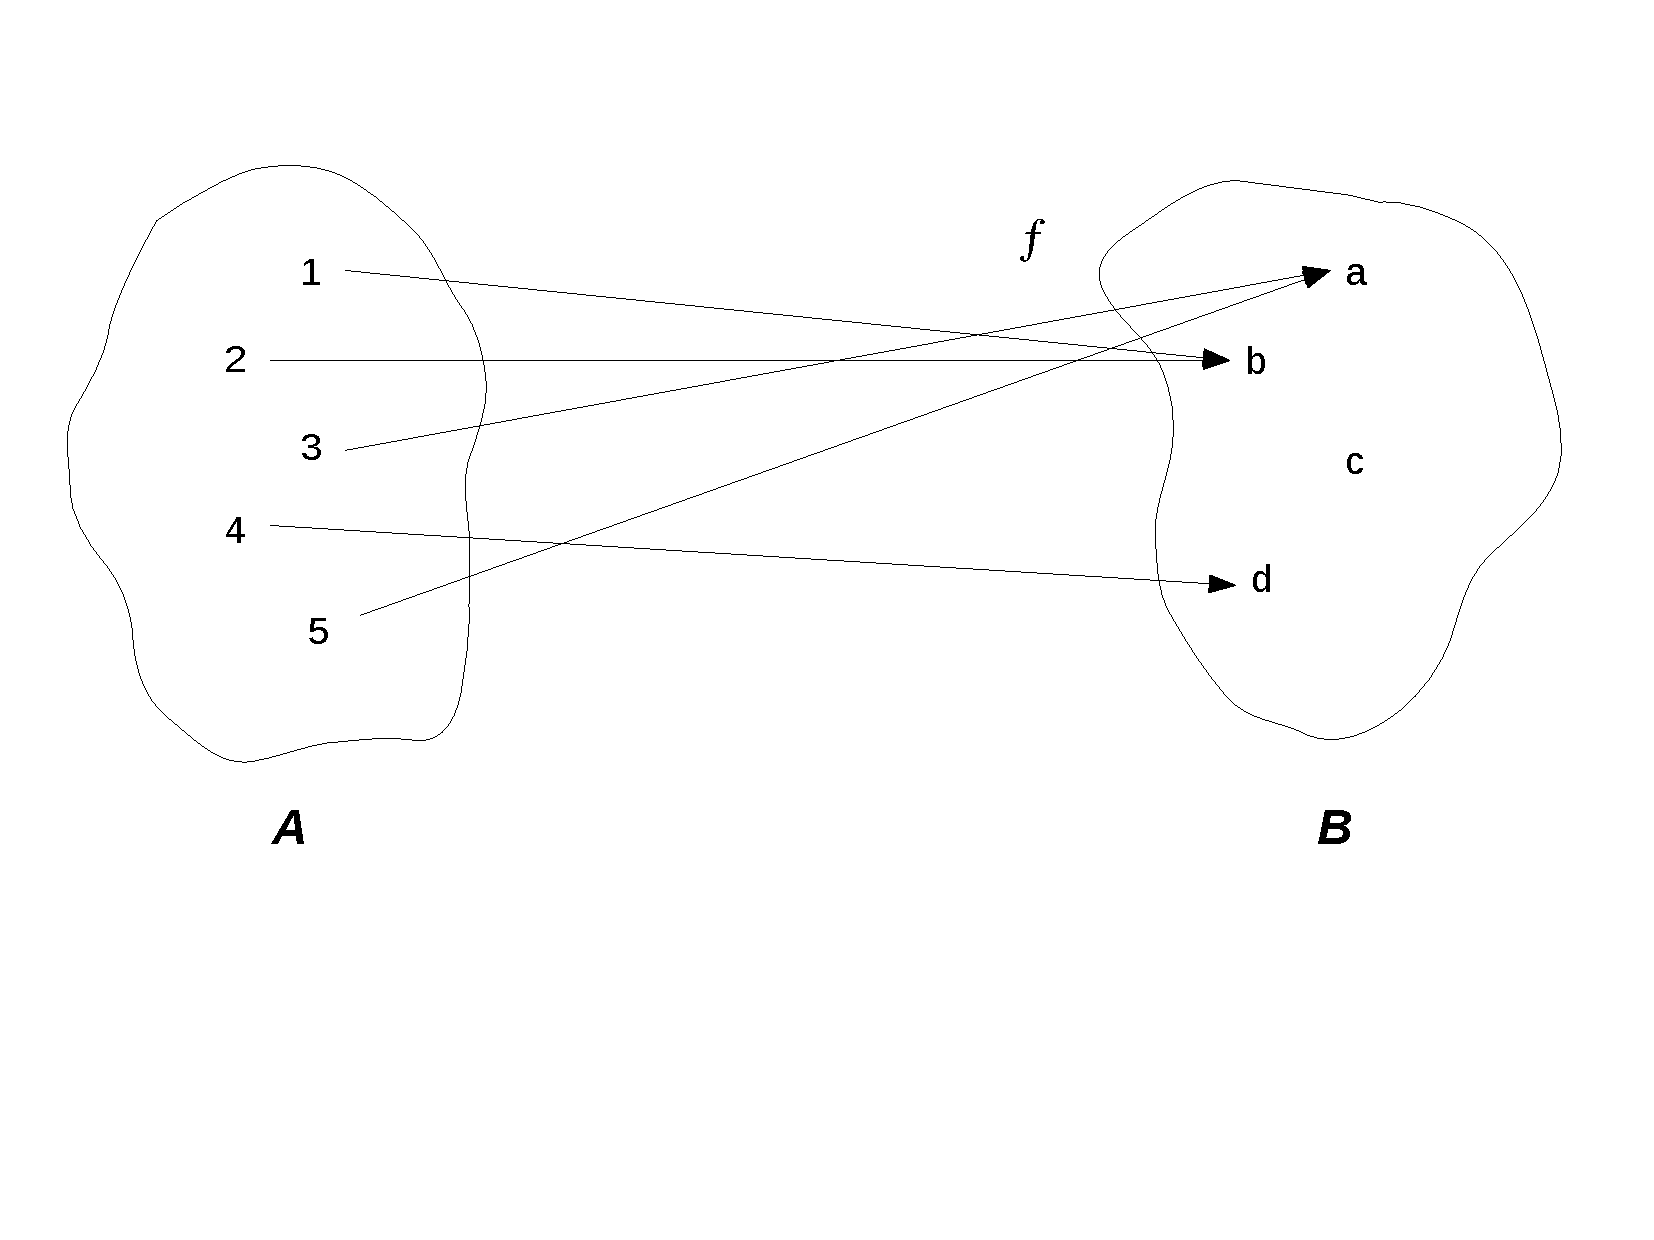
\includegraphics[width=12cm,trim={0.9cm 6.4cm 0.9cm 2.7cm},clip]{./figuras/figure26.pdf}
\end{center}
\end{figure}

Ent\ao a imagem de $2$ \'e $b$, a pr\'e-imagem de $a$ \'e $5$ (outra pr\'e-imagem de $5$ \'e $3$), $c$ n\ao tem pr\'e-imagem.

O seguinte teorema \'e \'util para determinar quando duas fun\coes s\ao iguais:
\begin{teob}
Sejam $f:A\to B$ e $g:A\to B$. Ent\ao $f=g$ se e somente se $\forall x\in A, f(x)=g(x)$.
\end{teob}
\begin{proof}
Primeiro, suponha que $f=g$ e seja $z\in A$. Ent\ao $\exists y\in B\ni (z,y)\in f$. Mas como $f=g$, $(z,y)\in g$. Assim $y=g(z)$ portanto $f(z)=g(z)$.

Agora, suponha que $\forall x\in A, f(x)=g(x)$. Como fun\coes s\ao rela\coes e rela\coes s\ao conjuntos de pares ordenados, para mostrar que $f=g$ devemos mostrar que s\ao iguais como conjuntos de pares ordenados. Para este fim, seja $(w,z)\in f$. Ent\ao $z=f(w)=g(w)$, portanto $(w,z)\in g$ e assim temos que $f\subseteq g$. Trocando $f$ por $g$ no argumento acima, mostramos que $g\subseteq f$. Assim segue que $f=g$. 
\end{proof}
\\

Existem certas propriedades que fun\coes podem ou n\ao ter que aparecem com frequ\^encia suficiente para terem um nome. Algumas destas s\ao dadas abaixo.
\begin{definb}
Seja $f:A\to B$. Ent\ao
\begin{enumerate}[{\bf a)}]
\item Dizemos que $f$ \'e injetora\index{Fun\caoi!Injetora} se e somente se $\forall w,z\in A, f(w)=f(z)$ implica $w=z$. 
\item Dizemos que $f$ \'e sobrejetora\index{Fun\caoi!Sobrejetora} se e somente se $\Ima(f)=B$.
\item Dizemos que $f$ \'e bijetora\index{Fun\caoi!Bijetora} (ou uma correspond\^encia um a um) se e somente se $f$ \'e injetora e sobrejetora.
\end{enumerate}
\end{definb}
A figuras abaixo ilustram as v\'arias possibilidades:

%
%
%
%
%
%
%
%
%
%

Recorde que como fun\coes s\ao rela\cois, elas t\^em inversas que s\ao rela\cois. Assim, podemos falar de inversa de qualquer fun\caoi, mas n\ao h\'a nenhuma raz\ao para esperar que a inversa de uma fun\cao ser\'a uma fun\caoi. Acontece que correspond\^encias um a um (bije\cois) s\ao particularmente importantes porque elas s\ao aquelas fun\coes cujas inversas tamb\'em s\ao fun\cois. Abaixo enunciamos e demonstramos este fato:
\begin{teob}\label{functeo13}
Seja $f:A\to B$. Ent\ao $f^{-1}:B\to A$ se e somente se $f$ \'e uma bije\cao (correspond\^encia um a um).
\end{teob}
\begin{proof}
Primeiro, suponha que $f^{-1}$ seja uma fun\cao de $B$ em $A$. Devemos mostrar que $f$ \'e injetora e sobrejetora. Suponha que $f(x)=f(y)=z$. Isto significa $(x,z)\in f$ e $(y,z)\in f$. Consequentemente, $f^{-1}(z)=x$ e $f^{-1}(z)=y$. Mas $f^{-1}$ \'e uma fun\caoi, portanto $x=y$ e assim $f$ \'e injetora. Para mostrar que $f$ \'e sobrejetora, seja $y\in B$. En\tao como $\Dom(f^{1})=B$, existe $x\in A$ tal que $f^{-1}(y)=x$. Assim $(y,x)\in f^{-1}$ que significa que $(x,y)\in f$ portanto $\Ima(f)=B$.

Agora, suponha que $f$ seja injetora e sobrejetora. Devemos mostrar que $f^{-1}$ \'e uma fun\cao de $B$ em $A$, isto \'e, devemos mostrar que $\Dom(f^{-1})=B$ e que se $(y,x)\in f^{-1}$ e $(y,z)\in f^{-1}$, ent\ao $x=z$. Primeiro, seja $y\in B$. Ent\ao como $f$ \'e sobrejetora, existe $x\in A$ tal que $f(x)=y$ ou $(x,y)\in f$. Assim $(y,x)\in f^{-1}$ portanto $\Dom(f^{-1})=B$. Aogra, suponha qye $(y,x)\in f^{-1}$ e $(y,z)\in f^{-1}$. Ent\ao $f(x)=y$ e $f(z)=y$. Mas como $f$ \'e injetora, isto implica que $x=z$ e consequentemente $f^{-1}$ \'e uma fun\caoi. 
\end{proof}
\\

Vale a pena mencionar que foi a injetividade de $f$ que deu a $f^{-1}$ a propriedade de fun\cao e a sobrejetividade de $f$ gerou o fato que $\Dom(f^{-1})=B$. Devemos ser um pouco cudadosos sobre exatamente o que o teorema diz. Suponha que $f:A\to B$ \'e uma fun\cao injetora mas n\ao uma fun\cao sobrejetora. Ent\ao $f^{-1}$ \'e uma funcaoi, mas n\ao de $B$ em $A$ e sim $f^{-1}:\Ima(f)\to A$.

Poder\ih amos, de fato, ter mostrado um pouco mais sobre $f^{-1}$ no teorema \ref{functeo13}, que $f^{-1}$ \'e tamb\'em uma bije\caoi. Uma demonstra\cao direta \'e poss\ih vel seguindo a demonstra\cao aicma, mas para checar nosso entendimento da nota\cao funcional, considere a seguinte demosntra\caoi:
\begin{teob}\label{functeo14}
Se $f:A\to B$ \'e injetora e sobrejetora ent\ao $f^{-1}:B\to A$ \'e uma bije\caoi.
\end{teob}
\begin{proof}
Usaremos o teorema acima duas vezes: primeiro, o teorema nos diz que $f^{-1}$ \'e uma fun\cao de $B$ em $A$. Agora, trocando os pap\'eis de $f$ e $f^{-1}$, o teorema tamb\'em diz que $(f^{-1})^{-1}$ \'e uma fun\caoi, ent\ao $f^{-1}$ deve ser injetora e sobrejetora. Mas $(f^{-1})^{-1}=f$.
\end{proof}
\\

No excerc\ih cio \ref{funcexerc3} abaixo, o leitor ir\'a demonstrar que a composi\cao de fun\coes \'e novamente uma fun\caoi. Usando este fato, se $f:A\to B$ e $g:B\to C$ ent\ao $(g\bola f):A\to C$. Para ver como nossa nota\cao funcional pode ser usada com a composi\cao de fun\cois, regressemos a deifni\cao de composi\cao de rela\cois. Se $(g\bola f)(x)=z$, ent\ao $(x,z)\in (g\bola f)$ que significa que existe um $y\in B$ tal que $(x,y)\in f$ e $(y,z)\in g$. Consequentemente, $f(x)=y$ e $g(y)=z$. Portanto, $z=g(y)=g(f(x))$ ou $(g\bola y)(x)=g(f(x))$, a nota\cao de composi\cao que usamos em c\'aculo. Agora o leitor pode ver porque escrevemos a composi\cao de rela\coes na ordem que fazemos, de mode que quando escrevemos composi\cao de fun\coes a ordem est\'a de acordo com nossa nota\cao funcional usual. (Digress\aoi: algumas pessoas (principalmente algebristas) contornam esta dificuldade traçando suas nota\coes funcionais, ao inv\'es de $f(x)$, eles escrevem $xf$, que resolve este problema, mas gera outros. Mesmo o mundo inventado das nota\coes matem\'aticas n\ao est\'a livre de dificuldades!)

Como fun\coes s\ao rela\coes podemos compor-las e os resultados que demonstramos para rela\coes continuam v\'alidos. Se $f,g$ s\ao fun\coes com dom\ih nios e imagens adequados, $(g\bola f)^{-1}=f^{-1}\bola g^{-1}$, embora $(g\bola f)^{-1}$, $f^{-1}$ e $g^{-1}$ possam n\ao serem fun\cois. O teorema \ref{functeo14} nos diz que se $f,g$ s\ao bije\cois, ent\ao $f^{-1}$ e $g^{-1}$ ser\ao fun\cois. Para completar nossa vis\ao sobre esse tema, provaremos mais dois teoremas sobre composi\cao de inversas de fun\cois.
\begin{teob}\label{functeo15}
Sejam $f:A\to B$ e $g:B\to C$ bije\cois. Ent\ao $g\bola f:A\to C$ \'e uma bije\caoi. 
\end{teob}
\begin{proof}
Contando com os resultados do excerc\ih cio \ref{funcexerc3} abaixo, assumiremos que $g\bola f$ \'e uma fun\cao de $A$ a $C$, portanto precisamos apenas mostrar que \'e uma bije\caoi. Primeiro, suponha que exista $x,y\in A$ tais que $g\bola f(x)=g\bola f(y)$. Assim, $g(f(x))=g(f(y))$. Mas $g$ \'e injetora, portanto $f(x)=f(y)$. Agora, o fato que $f$ \'e injetora nos diz que $x=y$, logo $g\bola f$ \'e injetora. Para mostrar que $g\bola f$ \'e sobrejetora, seja $z\in C$. Como $g$ \'e sobrejetora, existe $y\in B$ tal que $g(y)=z$. Mas $f$ \'e sobrejetora ent\ao existe $x\in A$ tal que $f(x)=y$. Assim, $z=g(y)=g(f(x))=g\bola f(x)$, logo $g\bola f$ \'e sobrejetora.
\end{proof}
\\

A demonstra\cao acima \'e uma t\ih pica demosntra\cao que mostra que uma certa fun\cao \'e injetora e sobrejetora. Para ter certeza que entendemos a forma deste tipo de demonstra\caoi, vamos dar uma olhada mais de perto. Suponha que $f:A\to B$. Uma demonstra\cao direta para mostrar que $f$ \'e injetora seria tomar a forma: Seja $x,y\in A$, com $f(x)=f(y)$.
\\
\ldots
\\ 
``alguma coisa ou outra dependendo de $f$''
\\
\ldots
\\
portanto $x=y$ e assim $f$ \'e injetora.

A demonstra\cao por contrapositiva seria da forma: Sejam $x,y\in A$, com $x\neq y$.
\\
\ldots
\\ 
``alguma coisa ou outra dependendo de $f$''
\\
\ldots
\\
portanto $f(x)\neq f(y)$ e assim $f$ \'e injetora.

A demonstra\cao direta para mostrar que $f$ \'e sobrejetora se pareceria como: Seja $y\in B$.
\\
\ldots
\\ 
``alguma coisa ou outra dependendo de $f$''
\\
\ldots
\\
portanto existe $x\in A$ tal que $f(x)=y$ e $f$ \'e sobrejetiva.

Resumo: para mostrar que $f$ \'e injetora, devemos mostrar que elementos distintos em um dom\ih nio t\^em imagens distintas e para mostrar que $f$ \'e sobrejetora, devemos mostrar que todos elementos de $B$ t\^em uma pr\'e-imagem.

Como exemplo, vamos mostrar que $f:\mathbb{R}\to\mathbb{R}$ dada por $f(x)=ax+b$, com $a\neq 0$ \'e uma bije\caoi. Primeiro, uma demonstra\cao direta que $f$ \'e injetora. Sejam $x,y\in\mathbb{R}$ com $f(x)=f(y)$. Ent\ao $ax+b=ay+b$ que implica que $ax=ay$. Como $a\neq 0$, temos $x=y$ e portanto $f$ \'e injetora. A demonstra\cao por contrapositiva deste fato seria: Sejam $x,y\in\mathbb{R}$ com $x\neq y$. Ent\ao como $a\neq 0$, $ax\neq ay$ portanto temos que $ax+b\neq ay+b$, logo $f(x)\neq f(y)$. Para mostrar que $f$ \'e sobrejetora, seja $z\in\mathbb{R}$. Ent\ao $(z-b)/a$ \'e tamb\'em um elemento de $\mathbb{R}$ (pois $a\neq 0$) e
\[
f\left(\frac{z-b}{a}\right)= a\left(\frac{z-b}{a}\right)+b=z-b+b=z.
\] 
portanto $f$ \'e sobrejtora. Devemos notar que a escolha de $(z-b)/a$ n\ao veio do nada, foi o resultado de resolver d equa\cao $f(x)=ax+b=z$ para $x$.
\begin{teob}\label{functeo16}
Sejam $f:A\to B$ e $g:B\to C$ bije\cois. Ent\ao $(g\bola f)^{-1}:C\to A$ e $\forall x\in C$, $(g\bola f)^{-1}(x)=(f^{-1}\bola g^{-1})(x)=f^{-1}(g^{-1}(x))$. 
\end{teob}
\begin{proof}
J\'a fizemos a maior parte do trabalho, assim devemos apenas fazer algumas observa\cois. Primeiro, como $f$ e $g$ s\ao bije\cois, $g\bola f$ tamb\'em \'e uma bije\caoi, portanto $(g\bola f)^{-1}$ \'e uma fun\cao de $C$ em $A$. Das rela\coes sabemos que, $(g\bola f)^{-1}=(f^{-1}\bola g^{-1}$ e como $f^{-1}$ e $g^{-1}$ s\ao fun\coes tamb\'em, o resultado segue.
\end{proof}
\\

Note que a rela\cao identidade em $A$, $I_A$, \'e uma fun\cao de $A$ em $A$ a qual chamaremos de {\it fun\cao identidade}.\index{Fun\caoi!Identidade} Usando nossa nota\cao funcional, $I_A(x)=x$ para todo $x\in A$. A raz\ao para este nome (e para o nome inversa) ficar\'a mais claro no r\'oximo teorema.
\begin{teob}\label{functeo17}
Seja $f:A\to B$. Ent\aoi
\begin{enumerate}[{\bf a)}]
\item $f\bola I_A=f$. 
\item $I_B\bola f=f$.
\item Se $f$ \'e uma bije\cao ent\ao $f^{1}\bola f=I_A$ (ou $\forall x\in A, f^{1}(f(x))=x$) e $f\bola f^{1}=I_B$ (or $\forall x\in B, f(f^{1}(x))=x$).
\end{enumerate}
\end{teob}
\begin{proof}
Itens a) e b) seguem facilmente, para isso suponha que $x\in A$. Ent\ao $f\bola I_A(x)=f(I_A(x))=f(x)$ e $I_B\bola f(x)=I_B(f(x))=f(x)$. Para c), primeiro observe que como $f$ \'e uma bije\caoi, $f^{-1}$ \'e uma fun\caoi, logo $f(x)=y$ se e somente se $f^{-1}(y)=x$. Agora, seja $x\in A$ e suponha que $f(x)=y$. En\tao $(f^{-1}\bola f)(x)=f^{-1}(f(x))=f^{-1}(y)=x=I_A(x)$. Para a segunda asser\caoi, seja $x\in B$ e suponha que $f^{-1}(x)=y$. Assim, $(f\bola f^{-1})(x)=f(f^{-1}(x))=f(y)=x=I_B(x)$.
\end{proof}
\\

\paragraph{Excerc\ih cios \ref{funcoes}}

\begin{enumerate}[{\bf 1.}]

%excercicio1
\item Seja $A=\{1,2,3,4,5,6\}$ e seja $f:A\to A$ dada por 
\begin{equation*}
 f(x)=\left\{ \begin{array}{lc}
x+1, & \textrm{ se $x\neq 6$;} \\
1,    & \textrm{ se $x=    6$.} \\
\end{array}\right.   
\end{equation*}
\begin{enumerate}[a)]
\item Encontre $f(3)$, $f(6)$, $f\bola f(3)$, $f(f(2))$. 
\item Encontre a pr\'e-imagem de $2$ e $1$.
\item Mostre que $f$ \'e bijetora.
\end{enumerate}

%excercicio2
\item Mostre que $f:\mathbb{R}\to\mathbb{R}$ dad por $f(x)=x^3$ \'e injetora e sobrejetora, enquanto que $g:\mathbb{R}\to\mathbb{R}$ dada por $g(x)=x^2-1$ n\ao \'e injetora nem sobrejetora. 

%excercicio3
\item\label{funcexerc3} Suponha $f:A\to B$ e $g:B\to C$. Mostre que $g\bola f:A\to C$.

%excercicio4
\item \begin{enumerate}[a)]
\item Sejam $A,B$ e $f:A\to B$ dados por:
\begin{equation*}
 \begin{aligned}
A=&\{1,2,3,4\},\\
B=&\{1,2,3,\},\\
f=&\{(1,3),(2,1),(3,1),(4,2)\}.
 \end{aligned}
\end{equation*}
Encontre $f^{-1}\bola f$.
\item Sejam $A,B$ conjuntos n\ao vazios e $f:A\to B$. Mostre que $f^{-1}\bola f$ \'e uma rela\cao de equival\^encia em $A$. (Note que $f^{-1}$ pode ou n\ao ser uma fun\caoi). Tamb\'em mostre que $[x]_{f^{-1}\bola f}=\{y: f(x)=f(y)\}$.
\end{enumerate}

%excercicio5
\item Seja $f:A\to B$. Prove que
\begin{enumerate}[a)]
\item $f$ \'e injetora se e somente se existe $g:B\to A$ tal que $g\bola f=I_A$.
\item $f$ \'e sobrejetora se e somente se existe $g:B\to A$ tal que $f\bola g=I_B$.
\item $f$ \'e sobrejetora se e somente se $f\bola f^{-1}=I_B$.
\end{enumerate}

%excercicio6
\item Sejam $f:A\to B$ e $g:B\to A$. Mostre que se $g\bola f=I_A$ e $f\bola g=I_B$ ent\ao $f$ \'e uma bije\cao e $g=f^{-1}$

%excercicio7
\item Seja $R$ uma rela\cao de equival\^encia em um conjunto n\ao vazio $A$. Definimos a rela\cao $\alpha$ de $A$ em $[A]_R$ por
\[
\alpha=\{(x,[x]_R): x\in A\}.
\]
\begin{enumerate}[a)]
\item Mostre que $\alpha:A\to [A]_R$.
\item Mostre que $\alpha$ \'e sobrejetora.
\item Sob quais condi\coes $\alpha$ ser\'a injetora?
\end{enumerate}

%excercicio8
\item Seja $f:A\to A$. Suponha que $f$ tamb\'em seja uma rela\cao de equival\^encia. O que podemos dizer sobre $f$? 

%excercicio9
\item Sejam $f:A\to B$ e $g:A\to B$. Demonstre ou d\^e contraexemplos para as seguintes conjecturas:
\begin{enumerate}[a)]
\item $f\uni g:A\to B$.
\item $f\inter g:A\to B$.
\item $f\uni g:A\to B$ implica $f=g$.
\item $f\inter g:A\to B$ implica $f=g$.
\end{enumerate}

%excercicio10
\item Seja $f:A\to B$ e $g:C\to D$, com $A\inter C=\varnothing$. [Para refrescar sua mem\'oria sobre restri\cois, veja o excerc\ih cio \ref{relexer13} da se\cao \ref{relacoes}]. 
\begin{enumerate}[a)]
\item Mostre que $f\uni g:A\uni C\to B\uni D$.
\item Mostre que $f\uni g|_A=f$ e $f\uni g|_C=g$. 
\end{enumerate}

%excercicio11
\item Seja $f:\mathbb{R}\to\mathbb{R}$ definida por $f(x)=\textrm{sen}(x).$
\begin{enumerate}[a)]
\item Mostre que $f$ n\ao \'e injetora.
\item Mostre que $f|_{[\pi/2,\pi/2]}$ \'e injetora.
\end{enumerate}

%excercicio12
\item Seja $A$ um conjunto n\ao vazio e seja 
\[
\Psi=\{\phi: \phi \textrm{ \'e uma parti\cao de } A\}.
\] 
Lembre-se que $\preceq$ (mais fino que) \'e uma rela\cao de ordem parcial em $\Psi$. Seja
\[
\Re=\{R: R \textrm{ \'e uma rela\cao de equival\^encia em } A\}.
\]
Sabemos que existe uma bije\cao entre os elementos de $\Psi$ e $\Re$, assim denotemos a rela\cao de equival\^encia associada com a parti\cao $\theta$ por $R_{\theta}$. Definimos s rela\cao $\sqsubseteq$ em $\Re$ por
\[
R_{\phi}\sqsubseteq R_{\theta} \textrm{ se e somente se } \phi \preceq \theta.
\]
\begin{enumerate}[a)]
\item Mostre que $\sqsubseteq$ \'e uma ordem parcial em $\Re$.
\item Mostre (ou d\^e um contraexemplo):
\[
R_{\phi}\sqsubseteq R_{\theta} \textrm{ se e somente se } R_{\phi}\subseteq R_{\theta}.
\]
\end{enumerate}

%excercicio13
\item Suponha que $f:A\to B$ e $g:B\to C$, onde $A,B$ e $C$ s\ao conjuntos n\ao vazios. Demonstre ou d\^e contraexemplos para as seguintes conjecturas:
\begin{enumerate}[a)]
\item $g\bola f$ bije\cao implica que $f$ \'e injetora. 
\item $g\bola f$ bije\cao implica que $f$ \'e sobrejetora.
\item $g\bola f$ bije\cao implica que $g$ \'e sobrejetora.
\item $g\bola f$ bije\cao implica que $g$ \'e injetora.
\end{enumerate}

%excercicio14
\item Seja $f:A\to B$, com $R$ uma ordem total estrita em $A$ e $S$ uma ordem total estrita em $B$. Dizemos que $f$ \'e {\it monot\^onica}\index{Fun\caoi!Monot\^onica} se e somente se $\forall x,y\in A,$ $xRy$ implica $f(x)Sf(y)$.
\begin{enumerate}[a)]
\item Com a ordem usual ($<$) em $\mathbb{R}$, de um exemplo de uma fun\cao que seja monot\^onica.
\item Com a ordem usual ($<$) em $\mathbb{R}$, de um exemplo de uma fun\cao que n\ao seja monot\^onica.
\item Se $f:A\to B$ \'e monot\^onica, mostre que $f$ \'e injetora.
\end{enumerate}

%excercicio15
\item {\bf Acredite se quiser:}  

\noindent \textit{\textbf{Conjectura:}} Seja $f:A\to B$ e seja $R$ uma ordem total estrita em $A$. Definimos a rela\cao $S$ em $B$ por
\[
xSy \leftrightarrow \exists a,b\in A \ni aRb\ee f(a)=x,f(b)=y.
\]
Ent\ao $S$ \'e uma ordem parcial estrita.

\noindent \textit{\textbf{``Demonstra\caoi'':}} Suponha que $f$ e $ R$ s\ao como acima e $S$ \'e definida como indicado. Seja $x\in B$ com $xSx$. Mas isto significa que existe $a\in A$ tal que $f(a)=x$. Assim $aRa$, que \'e imposs\ih vel, pois $R$ \'e irreflexiva, portanto $S$ \'e irreflexiva. Agora, suponha $x,y,z\in B$ com $xSy$, $ySz$. Ent\ao existem $a,b,c\in A$ tais que $f(a)=x$, $f(b)=y$ e $f(c)=z$ e $aRb$ e $bRc$. Como $R$ \'e transitiva, $aRc$ e portanto $xSz$, logo $S$ \'e transitiva.

\noindent \textit{\textbf{``Contraexemplo'':}} Sejam $A=\{1,2,3\}$, $B=\{1,2,3,4\}$ e $f:A\to B$ dada por $f(1)=1$, $f(2)=1$ e $f(3)=4$. Suponha,
\[
R=\{(1,2),(2,3),(1,3)\}
\]
Ent\ao $S=\{(1,2),(1,4)\}$, que \'e transitiva mas n\ao irreflexiva.

%excercicio16
\item {\bf Acredite se quiser:}  

\noindent \textit{\textbf{Conjectura:}} Seja $f:A\to B$ e $g:B\to A$. Se $g\bola f=I_A$ ent\ao $g=f^{-1}$.

\noindent \textit{\textbf{``Demonstra\caoi'':}} Sejam $f,g$ como acima e seja $x\in B$. Suponha que $y\in A$ \'e tal que $(x,y)\in g$. Seja $x\in B$ tal que $(y,z) \in f$. Como $g\bola f=I_A$, $(x,y)\in g$. Mas $(x,y)\in g$ e $g$ \'e uma fun\caoi, portanto $x=z$. Assim, $(x,y)\in f^{-1}$, logo $g\subseteq f^{-1}$. Agora suponha que $(x,y)\in f^{-1}$. Ent\ao $(y,x)\in f$. Como $g\bola f=I_A$, $(x,y)\in g$, logo $f^{-1}\subseteq g$ e portanto temos que $g=f^{-1}$.

\noindent \textit{\textbf{``Contraexemplo'':}} Sejam $A=\{1,2,3\}$, $B=\{1,2,3,4\}$ com
\[
f=\{(1,2),(2,1),(3,3)\}
\]
\[
g=\{(2,1),(1,2),(3,3),(4,3)\}
\]
Ent\ao $g\bola f=I_A$ mas $g\neq f^{-1}$, pois $(4,3)\in g$.

%excercicio17
\item {\bf Acredite se quiser:}  

\noindent \textit{\textbf{Conjectura:}} Seja $f:A\to B$. Se $f^{-1}\bola f=I_A$ ent\ao $f$ \'e injetora.

\noindent \textit{\textbf{``Demonstra\caoi'':}} Suponha que $f$ \'e como descrito acima e $x,y\in A$ com $f(x)=f(y)=z$. Ent\ao $f^{-1}(z)=x$ e $f^{-1}(z)=y$. Mas $f^{-1}$ \'e uma fun\caoi, portanto $x=y$ e assim $f$ \'e injetora.

\noindent \textit{\textbf{``Contraexemplo'':}} Sejam $A=\{a,b,c\}$ e $B=\{1,2,3\}$ com $f(a)=1$, $f(b)=2$ e $f(c)=2$. En\tao $f^{-1}=\{(1,a),(2,b),(2,c)\}$ mas $f$ n\ao \'e injetora.
\end{enumerate}
%%%%%%%%%%%%%%%%%%%%%%%%%%%%%%%%%%%%%%%%%%%%%%%%%%%%%%%%%%%%%%%%%%%%%%%%%%%%%%%%%%%%%%%%%%%%

\section{Mais Fun\cois}\label{mfuncoes}

Podemos extender a ideia de fun\cao de uma forma natural de elementos individuais do dom\ih nio em subconjuntos do dom\ih nio, isto \'e, $f:A\to B$ pode ser extendido para $f:\mathbb{P}(A)\to \mathbb{P}(B)$.
\begin{definb}
Seja $f:A\to B$. Se $C\subseteq A$ ent\ao definimos $f(C)=\{f(x): x\in C\}$. Se $D\subseteq B$ en\tao $f^{-1}(D)=\{x: f(x)\in D\}$. $f(C)$ \'e chamada a imagem de $C$ e $f^{-1}(D)$ \'e chamada a pr\'e-imagem de $D$.
\end{definb}

Por exemplo, seja $f:A\to B$ onde $A=\{1,2,3,4\}$, $B=\{1,3,5\}$ e $f$ dada por $f(1)=1$, $f(2)=1$, $f(3)=5$ e $f(4)=5$. Ent\ao
\begin{equation*}
 \begin{aligned}
f(\{1,3\})=&\{1,5\},\\
f(\{1,2\})=&\{1\},\\
f^{-1}(\{1\})=&\{1,2\},\\
f^{-1}(\{4\})=&\varnothing.
 \end{aligned}
\end{equation*}
Note que at\'e agora definimos alguns conjuntos: com $A,B,f,C,D$ como acima, $f(C)$ \'e um subconjunto de $B$ e $f^{-1}(D)$ \'e um subconjunto de $A$. Entretanto, podemos utilizar estas defini\coes de uma forma natural para definir algumas fun\coes (com o mesmo nome)
\[
f:\mathbb{P}(A)\to \mathbb{P}(B),
\]
\[
f^{-1}:\mathbb{P}(B)\to \mathbb{P}(A).
\]
Estas duas fun\coes induzidas por conjuntos t\^em muitas propriedades importantes (incluindo o fato de que elas s\ao fun\cois!), que em sua maioria ser\ao deixadas para os excerc\ih cios, mas provaremos uma aqui para dar uma dica de como s\ao estas demonstra\cois.
\begin{teob}
Seja $f:A\to B$ e sejam $C\subseteq D \subseteq B$. Ent\ao
\[
f^{-1}(C)\subseteq f^{-1}(D).
\]
\end{teob}
\begin{proof}
Seja $x\in f^{-1}(C)$. Ent\ao $x\in A$ e $f(x)\in C$. Como $C\subseteq D$, $f(x)\in D$. Mas isto significa que $x\in f^{-1}(D)$.
\end{proof}
\\

Todas as nossas familiares opera\coes aritm\'eticas ($+$, $-$, $\cdot$ e $\div$) s\ao funcois, assim como todos os conectivos l\'ogicos ($\ee$, $\ou$, $\rightarrow$ e $\leftrightarrow$) e todas opera\coes de conjuntos ($\inter$, $\uni$ e $-$). Temos um nome especial para fun\coes deste tipo:
\begin{definb}
Seja $A$ um conjunto. $\bullet$ \'e chamada {\it opera\cao bin\'aria}\index{Opera\cao Bin\'aria} em $A$ se e somente se 
\[
\bullet :A\times A\to A.
\]
\end{definb}

Assim vemos que a oper\cao bin\'aria em $A$ associa cada par de elementos de $A$ a um elemento de $A$. Por causa disso iremos nos afastarde nossa nota\cao funcional usual e escrever:
\[
a\cdot b=c \textrm{ ao inv\'es de } \cdot((a,b))=c.
\]

Por exemplo, com $+:\mathbb{R}\times\mathbb{R}\to\mathbb{R}$ (adi\cao de n\'umeros reais), escrevemos $2+3=5$ ao inv\'es de $+((2,3))=5$.

Existem muitas propriedades que as opera\coes bin\'arias podem ou n\ao ter:
\begin{definb}
Seja $\bullet$ uma opera\cao bin\'aria em um conjunto $A$. Ent\aoi:
\begin{enumerate}[{\bf a)}]
\item Dizemos que $\bullet$ \'e {\it comutativa}\index{Opera\cao Bin\'aria!Comutativa} se e somente se $\forall a,b\in A, a\bullet b=b\bullet a$.
\item Dizemos que $\bullet$ \'e {\it associativa}\index{Opera\cao Bin\'aria!Associativa} se e somente se $\forall a,b,c\in A, a\bullet(b\bullet c)=(a\bullet b)\bullet c$.
\item Dizemos que $e\in A$ \'e uma {\it identidade}\index{Opera\cao Bin\'aria!Identidade} para $\bullet$ se e somente se $\forall a\in A, a\bullet e=e\bullet a=a$.
\item Se $e$ \'e uma identidade para $\bullet$ e $x\in A$, dizemos que $x$ \'e {\it invert\ih vel}\index{Opera\cao Bin\'aria!Elemento Inverso} se e somente se $\exists y\in A \ni x\bullet y=y\bullet x=e$. Tal $y$ \'e chamado um {\it inverso} de $x$.
\item Dizemos que $a\in A$ \'e {\it idempotente}\index{Opera\cao Bin\'aria!Elemento Idempotente} para $\bullet$ se e somente se $a\cdot a=a$.
\end{enumerate}
\end{definb}

Alguns exemplos destas propriedades, $+$ em $\mathbb{R}$ \'e comutativa, associativa, tem $0$ como identidade e todo elemento \'e invert\ih vel (o inverso de $x$ \'e $-x$). O \'unico elemento idempotente \'e $0$. Por outro lado, $-$ em $\mathbb{R}$ n\ao \'e comutativo, n\ao \'e associativo, n\ao tem identidade e o \'unico elemento idempotente \'e $0$. $\uni$ em $\mathbb{P}(A)$ para algum conjunto $A$ \'e comutativo, associativo, $\varnothing$ \'e a identidade e cada elemento \'e idempotente.

Vamos demonstrar alguns poucos teoremas envolvendo oper\coes bin\'arias e deixar alguns outros para os ecerc\ih cios.
\begin{teob}
Seja $\bullet$ uma opera\cao bin\'aria em $A$. Ent\ao existe no m\'aximo uma identidade para $\bullet$.
\end{teob}
\begin{proof}
Suponha que $e$ e $e'$ s\ao ambos identidades para $\bullet$. Ent\ao
\[
e=e\bullet e'=e'
\]
Assim $e=e'$ e $\bullet$ pode ter no m\'aximo uma identidade.

\noindent [Nota: A primeira igualdade \'e v\'alida pois $e'$ \'e uma identidade e a segunda \'e v\'alida porque $e$ \'e uma identidade.] 
\end{proof}
\\

\begin{teob}\label{functeo20}
Se $\bullet$ \'e uma opera\cao bin\'aria associativa com identidade $e$ em $A$ e $x\in A$, ent\ao $x$ tem no m\'aximo um inverso.
\end{teob}
\begin{proof}
Suponha que $x\in A$ tem dois inversos, que chamaremos de $y$ e $y'$. Ent\ao
\[
x\bullet y=y\bullet x=e
\]
e
\[
x\bullet y'=y'\bullet x=e
\]
Assim,
\[
y=y\bullet e=y\bullet(x\bullet y')=(y\bullet x)\bullet y'=e\bullet y'=y'.
\]
\end{proof}
\\

Em virtude dos teoremas acima podemos falar em ``a'' identidade e ``o'' inverso de um elemento (se tais existem).

A \'ultima ideia que gostar\ih amos de introduzir nesta se\cao pode, de alguma forma, ser sutil, mas o esfor\cc o para entende-la ser\'a recompensado no futuro (por exemplo, quando o leitor estiver estudando em \'algebra o ``teorema fundamental de homomorfismos de grupos'').
\begin{teob}\label{functeo21}
Seja $f:A\to B$. Definimos a rela\cao $R$ em $A$ por $xRy$ se e somente se $f(x)=f(y)$. Ent\ao $R$ \'e uma rela\cao de equival\^encia em $A$ e consequentemente $[A]_R$ \'e uma parti\cao de $A$. Definimos duas novas fun\cois:
\begin{equation*}
 \begin{aligned}
&\alpha:A\to[A]_R \textrm{ por } \alpha(x)=[x]_R,\\
&f^{\ast}:[A]_R\to B \textrm{ por } f^{\ast}([x]_R)=f(x). 
 \end{aligned}
\end{equation*}
Ent\ao $f^{\ast}$ \'e injetora e $f=f^{\ast}\bola\alpha.$
\end{teob}
\begin{proof}
Ser\'a \'util manter a figura abaixo na mente durante nosso trabalho na demonstra\caoi.

\begin{figure}[h]
\begin{center}
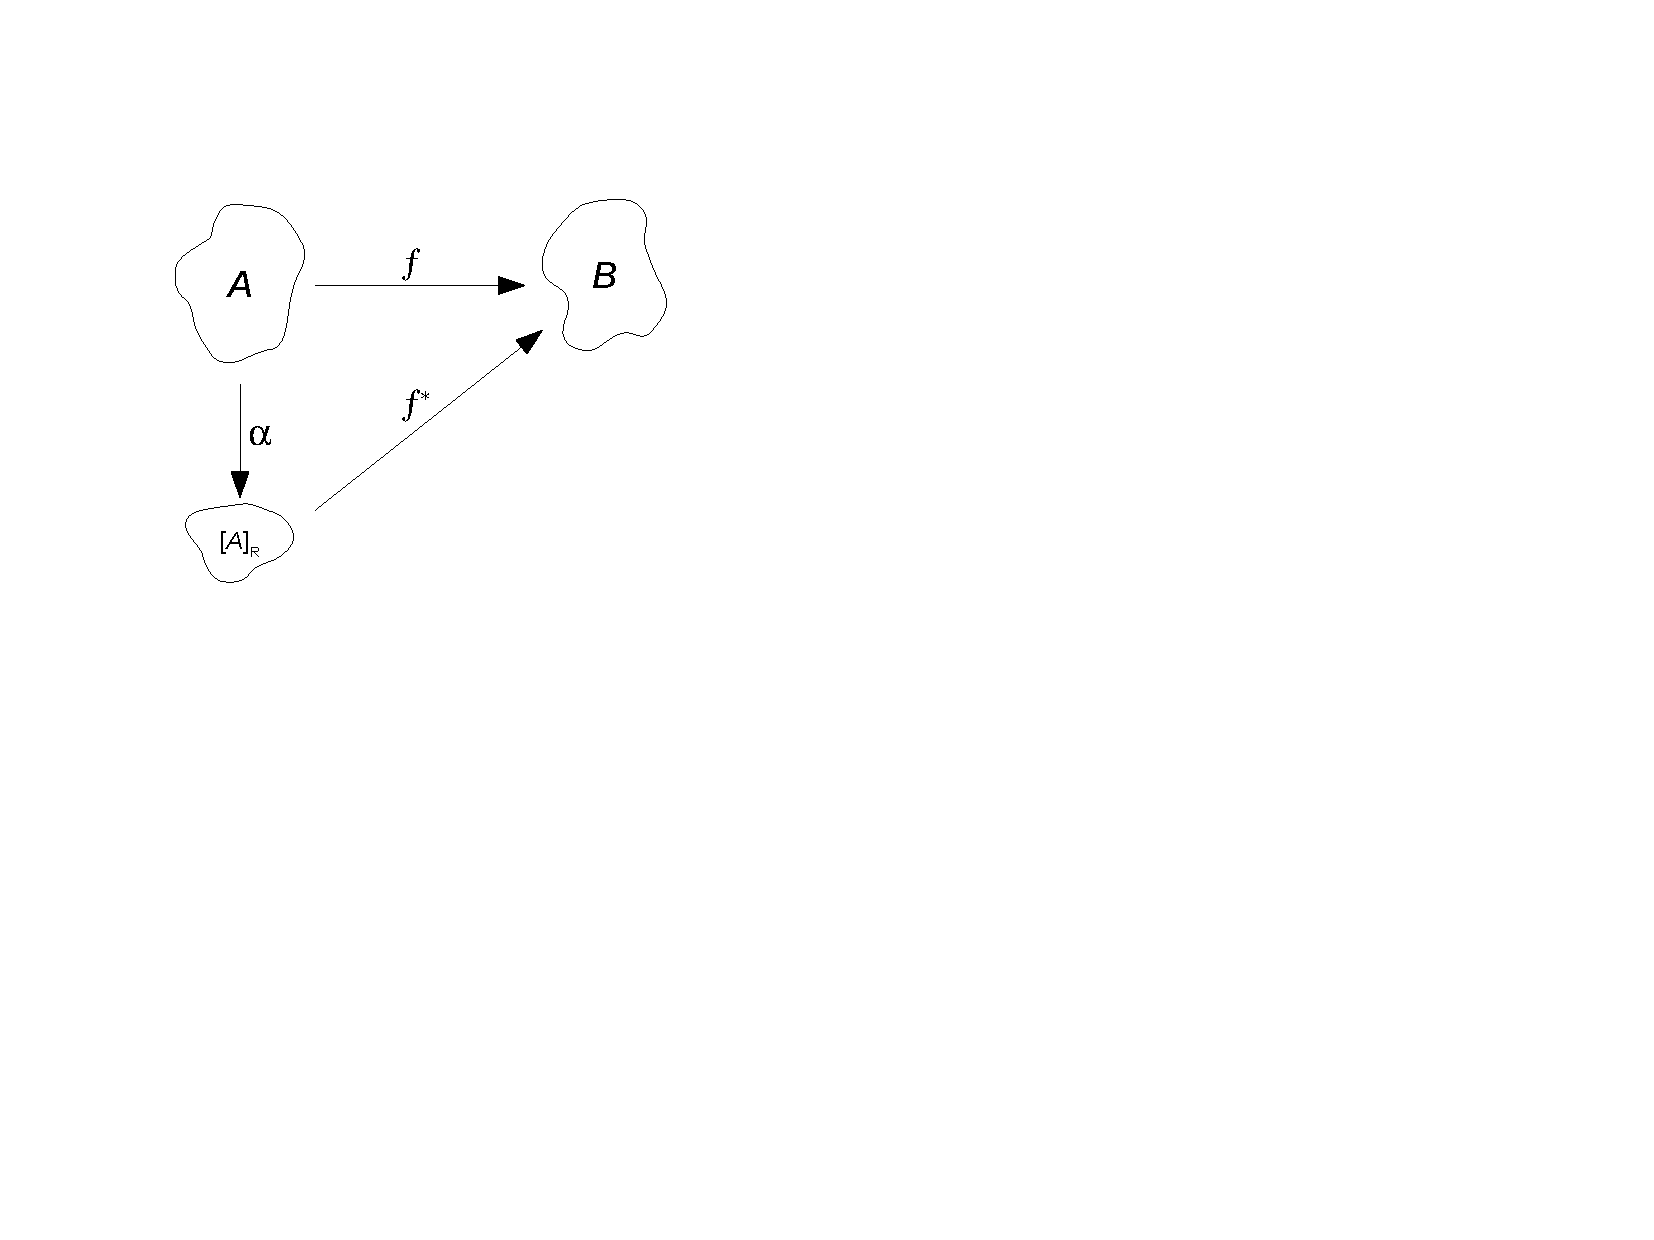
\includegraphics[width=15cm,trim={1.3cm 11.1cm 16cm 2.3cm},clip]{./figuras/figure28.pdf}
\end{center}
\end{figure}

Devemos observar que h\'a quatro coisas que devem ser provadas:
\begin{enumerate}[{\bf a)}]
\item $R$ \'e uma rela\cao de equival\^encia.
\item $f^{\ast}$ \'e uma fun\caoi.
\item $f^{\ast}$ \'e injetora.
\item $f=f^{\ast}\bola\alpha$. 
\end{enumerate}

Que $R$ \'e uma rela\cao de equival\^encia segue facilmente do fato que $=$ \'e uma rela\cao de equival\^encia em $B$, os detalhes s\ao deixados como excerc\ih cio. Que $f^{\ast}$ \'e uma fun\cao \'e um ponto mais sutil porque classes de equival\^encia est\ao envolvidas e $f^{\ast}$ est\'a definida de um representante da classe de equival\^encia. Para explicar isso um pouco mais, suponha $[x]_R=[y]_R$ com $x\neq y$. Para $f^{\ast}$ ser uma fun\cao e n\ao apenas uma rela\cao, necessitar\ih amos que $f^{\ast}([x]_R)=f^{\ast}([y]_R)$ (pois $[x]_R=[y]_R$) mas nossa defini\cao de $f^{\ast}$ \'e dada em termos dos representantes das classes de equival\^encia, isto \'e $f^{\ast}([x]_R)=f(x)$ enquanto $f^{\ast}([y]_R)=f(y)$. Obviamente, nossa \'unica esperan\cc a de livra-nos com sucesso desta dificuldade \'e ter $f(x)=f(y)$. Mas se lembrarmos que $xRy$ se e somente se $f(x)=f(y)$, vemos que $[x]_R=[y]_R$ implica que $f(x)=f(y)$ e $f^{\ast}$ \'e de fato uma fun\cao (\`as vezes dizemos que tal fun\cao definida em um conjunto de classe de equival\^encia est\'a ``bem definida''). Assim, tudo que resta demonstrar sobre $f^{\ast}$ \'e que $f^{\ast}$ \'e injetora. Suponha que, $f^{\ast}([x]_R)=f^{\ast}([y]_R)$. Ent\ao $f(x)=f(y)$ (da defini\cao de $f^{\ast}$), logo $xRy$ que significa $[x]_R=[y]_R$, portanto, $f^{\ast}$ \'e injetora. Para completar a demosntra\cao precisamos mostrar que $f=f^{\ast}\bola\alpha$. Seja $x\in A$. Ent\ao $(f^{\ast}\bola\alpha)(x)=f^{\ast}(\alpha(x))=f^{\ast}([x]_R)=f(x)$.
\end{proof}
\\

Para melhor entender o que est\'a acontecendo aqui, pode ajudar a perceber que a classe de equival\^encia $[x]_R$ \'e o conjunto de todos os elementos cuja imagem por $f$ \'e o mesmo de $x$. Assim podemos pensar na parti\cao $[A]_R$ como juntando todos estes elementos que t\^em a mesma imagem por $f$. Como um exemplo simples disso, considere $f:A\to B$ onde $A=\{1,2,3,4\}$, $B=\{1,3,5\}$ e $f$ \'e dada por $f(1)=1$, $f(2)=1$, $f(3)=5$ e $f(4)=5$. Neste caso (o leitor pode verificar)
\[
R=\{(1,1),(1,2),(2,2),(2,1),(3,3),(3,4),(4,4),(4,3)\}
\] 
logo $[1]_R=[2]_R=\{1,2\}$, $[3]_R=[4]_R=\{3,4\}$. Portanto, $[A]_R=\{[1]_R,[3]_R\}$ e $f^{\star}([1]_R)=1$ e $f^{\star}([3]_R)=5$.


\paragraph{Excerc\ih cios \ref{mfuncoes}}

\begin{enumerate}[{\bf 1.}]

%excercicio1
\item Sejam $A=\{1,2,3,4,5,6\}$, $B=\{2,3,4,5\}$ e $f:A\to B$ dada por $f(1)=f(4)=f(6)=3$; $f(2)=5$ e $f(3)=f(5)=4$. Encontre:
\begin{enumerate}[a)]
\item $f(\{1,2,3\})$, $f(A-\{2\})$ e $f(A)-\{2\}$.
\item $f^{-1}(\{3\})$, $f^{-1}(\{4,5\})$ e $f^{-1}(\{2\})$.
\item $f(\{1,2\}\inter \{2,6\})$ e $f(\{1,2\})\inter f(\{2,6\})$. 
\end{enumerate}

%excercicio2
\item Seja $f:A\to B$. Mostre que:
\begin{enumerate}[a)]
\item $C\subseteq D\subseteq A$ implica $f(C)\subseteq f(D)$.
\item $C\subseteq A$ e $D \subseteq A$ implica que $f(C\uni D)=f(C)\uni f(D)$. 
\item $C\subseteq B$ e $D \subseteq B$ implica que $f^{-1}(C\uni D)=f^{-1}(C)\uni f^{-1}(D)$.
\item $C\subseteq B$ e $D \subseteq B$ implica que $f^{-1}(C\inter D)=f^{-1}(C)\inter f^{-1}(D)$.
\item $C\subseteq A$ implica $C\subseteq f^{-1}(f(C))$ e d\^e um exemplo para mostrar que a igualdade n\ao vale.
\item $C\subseteq B$ implica $f(f^{-1}(C))\subseteq C$ e d\^e um exemplo para mostrar que a igualdade n\ao vale. 
\end{enumerate}

%excercicio3
\item Seja $f:A\to B$. Para distinguir entre $f$ e a extens\ao de $f$ para subconjuntos de $A$, vamos definir $f^{\ast}$ a rela\cao de $\mathbb{P}(A)$ em $\mathbb{P}(B)$ por
\[
f^{\ast}=\{(C,f(C)): C\in \mathbb{P}(A)\},
\]
e $(f^{-1})^{\ast}$ a rela\cao de $\mathbb{P}(B)$ em $\mathbb{P}(A)$ por
\[
(f^{-1})^{\ast}=\{(C,f^{-1}(C)): C\in \mathbb{P}(B)\}.
\]
\begin{enumerate}[a)]
\item Mostre que $f^{\ast}:\mathbb{P}(A)\to\mathbb{P}(B)$.
\item Mostre que $(f^{-1})^{\ast}:\mathbb{P}(B)\to\mathbb{P}(A)$.
\item Mostre que $f$ injetora se e somente se $f^{\ast}$ injetora.
\item Mostre que $f$ sobrejetora se e somente se $f^{\ast}$ sobrejetora.
\item Quando $(f^{-1})^{\ast}=(f^{\ast})^{-1}$?  
\end{enumerate}

%excercicio4
\item Seja $A$ um conjunto n\ao vazio e seja $F=\{f: f:A\to A\}$. Ent\ao $\bola$ (composi\cao de fun\caoi) \'e uma opera\cao bin\'aria em $F$. Para responder o que segue o leitor usar\'a alguns dos teoremas demonstrados anteriormente.
\begin{enumerate}[a)]
\item Mostre que $\bola$ \'e associativa. 
\item D\^e um exemplo para mostrar que $\bola$ n\ao \'e comutativa.
\item Mostre que $I_A$ \'e a identidade para $\bola$.
\item Quais elementos de $F$ t\^em inversa?
\item D\^e exemplos de fun\coes idempotentes.
\item Se $f$ \'e invert\ih vel e $f\bola g=f\bola h$, ent\ao $g=h$?
\item Mostre que se $f$ e $g$ s\ao invert\ih veis ent\ao $f\bola g$ \'e tamb\'em invert\ih vel. Qual \'e o inverso de $f\bola g$?
\end{enumerate}

Talvez agora os nomes identidade e inverso como usados com fun\coes assumem mais significado agora, para $I$ \'e a identidade de $\bola$ e $f^{-1}$ \'e o inverso de $f$.

%excercicio5
\item Seja $\bullet$ uma opera\cao bin\'aria em $A$. Mostre que:
\begin{enumerate}[a)]
\item Se $e$ \'e a identidade de $\bullet$ ent\ao $e$ \'e idempotente para $\bullet$.
\item Se $\bullet$ \'e associativa e comutativa e $a$ e $b$ s\ao ambos idempotentes para $\bullet$ ent\ao $a\bullet b$ \'e tamb\'em idempotente.
\item Se $\bullet$ \'e associativa e $x$ e $y$ s\ao invert\ih veis ent\ao $x\bullet y$ \'e tamb\'em idempotente. Expresse a inversa de $x\bullet y$ em termos das inversas de $x$ e $y$.
\end{enumerate}

%excercicio6
\item Seja $A$ um conjunto n\ao vazio. Ent\ao $\uni$, $\inter$ e $-$ s\ao opera\coes bin\'arias em $\mathbb{P}(A)$. O leitor pode quere citar os teoremas demonstrados anteriormente e outros excerc\i cios para trabalhar nos seguintes itens:
\begin{enumerate}[a)]
\item Mostre que $\uni$ e $\inter$ s\ao associativas e comutativas.
\item D\^e exemplos para mostrar que $-$ n\ao \'e nem associativa nem comutativa.
\item Mostre que cada elemento em $\mathbb{P}(A)$ \'e idempotente para $\uni$ e $\inter$.
\item Quais elementos s\ao idempotentes para $-$?
\item Quais elementos s\ao invert\ih veis para $\uni$, $\inter$ e $-$?
\end{enumerate}

%excercicio7
\item Seja $A$ um conjunto n\ao vazio. Definimos a opera\cao bin\'aria $\bullet$ em $\mathbb{P}(A)$ por
\[
X\bullet Y=(X-Y)\uni(Y-X).
\]
\begin{enumerate}[a)]
\item Mostre que $\bullet$ \'e comutativa.
\item Mostre que $\bullet$ \'e associativa.
\item Qual a identidade para $\bullet$?
\item Mostre que cada elemento pertencente a $\mathbb{P}(A)$ \'e invert\ih vel.
\item Se $X\subseteq A$, qual \'e o inverso de $X$ para $\bullet$? 
\end{enumerate}

%excercicio8
\item Seja $F=\{f: f:\mathbb{R}\to\mathbb{R}, f(x)=ax+b, a\neq 0\}$. [$F$ \'e o conjunto de todas as fun\coes lineare n\ao constantes de $\mathbb{R}$ em $\mathbb{R}$.]
\begin{enumerate}[a)]
\item Mostre que $\bola$ (composi\cao de fun\cois) \'e uma opera\cao bin\'aria em $F$.
\item Qual a identidade para $\bola$?
\item Quais elementos de $F$ s\ao invert\ih veis?
\item Se $f$ \'e invert\ih vel, qual a inversa de $f$?
\item Quais elementos de $F$ s\ao idempotentes? 
\end{enumerate}

%excercicio9
\item Suponha que $\bullet$ seja uma opera\cao bin\'aria associativa em $A$. Seja $x$ um elemento fixo pertencente a $A$. Definimos uma outra rela\cao bin\'aria $\bullet_x$ em $A$ por
\[
a\bullet_x b=a\bullet(x\bullet b).
\]
Mostre que $\bullet_x$ \'e associativa.

%excercicio10
\item Mostre que a rela\cao $R$ do teorema \ref{functeo21} \'e uma rela\cao de equival\^encia.

%excercicio11
\item Seja $\bullet$ uma opera\cao bin\'aria em $A$. Se $B\subseteq A$, podemos considerar que a restri\cao de $\bullet$ a $B$, $\bullet|_B$. Esta restri\cao pode ou n\ao ser uma opera\cao bin\'aria em $B$. Se $\bullet|_B$ for uma opera\cao bin\'aria em $B$, dizemos que $B$ \'e fechado com respeito a $\bullet$. 
\begin{enumerate}[a)]
\item D\^e uma defini\cao precisa da restri\cao mencionada acima.
\item Sejam $+,-$ as opera\coes alg\'ebricas usuais em $\mathbb{Z}$. Mostre que $\mathbb{N}$ \'e fechado com respeito a $+$, mas n\ao \'e fechado com respeiro a $-$.
\item Se $\bullet$ \'e uma opera\cao bin\'aria em $A$ com $B\subseteq A$, mostre que $B$ \'e fechado com respeito a $\bullet$ se e somente se 
\[
\{x\bullet y: x,y\in B\}\subseteq B.
\]
\end{enumerate}

%excercicio12
\item Seja $f:A\to B$. Mostre que $f$ pode ser decomposta em uma sobreje\caoi, uma bije\cao e uma inje\caoi, isto \'e, existem fun\coes $\alpha, \beta$ e $\gamma$ tais que $f=\gamma\bola\beta\bola\alpha$ onde $\alpha$ \'e uma sobrej\caoi, $\beta$ \'e uma bije\cao e $\gamma$ \'e uma inje\caoi. [Dica: veja o teorema \ref{functeo21}.]

%excercicio13
\item Em \'algebra com frequ\^encia usamos a regra ``igual adicionado a igual \'e igual'', ou mais precisamente, se $a,b,c,d\in\mathbb{R}$ com $a=b$ e $c=d$ ent\ao $a+c=b+d$. Prove que esta afirma\cao est\'a correta.

%excercicio14
\item {\bf Acredite se quiser:}  

\noindent \textit{\textbf{Conjectura:}} Seja $f:A\to B$ e $C,D\subseteq A$. Ent\ao $f(C\inter D)=f(C)\inter f(D)$.

\noindent \textit{\textbf{``Demonstra\caoi'':}} Sejam $C,D\in A$ e suponha $x\in f(C\inter D)$. Ent\ao existe $y\in C\inter D$ tal que $f(y)=x$. Claramente $y\in C$ e $y\in D$, assim $f(y)\in f(C)$ e $f(y)\in f(D)$, logo $x\in f(C)\inter f(D)$. Agora, suponha $x\in f(C)\inter f(D)$. Ent\ao existe $y\in C$ tal que $f(y)=x$ e existe $y\in D$ tal que $f(y)=x$. Mas $y\in C\inter D$, logo $x\in f(C\inter D)$. 

\noindent \textit{\textbf{``Contraexemplo'':}} Sejam $A=\{1,2\}$, $B=\{1,2,3\}$ e seja $f:A\to B$ dada por $f(1)=1$ e $f(2)=1$. Se $C\{a\}$ e $D=\{2\}$, ent\ao $f(C\inter D)\varnothing$ enquanto que $f(C)\inter f(D)=\{1\}$. 

%excercicio15
\item {\bf Acredite se quiser:}  

\noindent \textit{\textbf{Conjectura:}} Sejam $A$ e $B$ conjuntos com $f:A\to B$. Ent\ao $f^{-1}\bola f$ (estas s\ao as fun\coes induzidas por conjuntos) \'e uma rela\cao de equival\^encia em $\mathbb{P}(A)$.

\noindent \textit{\textbf{``Demonstra\caoi'':}} Sejam $A$, $B$ e $f$ como descritos acima e por conveni\^encia, vamos denotar a composi\cao de fun\coes induzidas por comjuntos, $f^{-1}\bola f$, por $R$. Seja $C\in \mathbb{P}(A)$. Como $f^{-1}(f(C))=C$, $(C,C)\in R$ e portanto $R$ \'e reflexiva. Se $C,D \in \mathbb{P}(A)$, com $(C,D)\in R$ ent\ao temos que $f^{-1}(f(C))=D$. Assim,
\[
f(D)=f^{-1}(f(C))=f^{-1}\bola f(C)=I_B(f(C))=f(C).
\]
Como $f(C)=f(D)$ ent\ao $f^{-1}(f(C))=f^{-1}(f(D))$ logo, $(D,C)\in R$ e portanto $R$ \'e sim\'etrica. Agora suponha que $(C,D)\in R$ e $(D,E)\in R$. Assim $f^{-1}(f(C))=D$ e $f^{-1}(f(D))=E$. Portanto,
\[
E=f^{-1}(f(D))= (f^{-1}\bola f)(f^{-1}\bola f(C))=f^{-1}\bola (f\bola f^{-1})\bola f(C)=f^{-1}\bola I_B(f(C))=f^{-1}(f(C))
\]
e assim $(C,E)\in R$ e portanto $R$ \'e transitiva, consequentemente uma rela\cao de equival\^encia.

\noindent \textit{\textbf{``Contraexemplo'':}} Sejam $A=\{1,2\}$, $B=\{1,2,3\}$ e $f:A\to B$ dada por $f(1)=1$ e $f(2)=1$. Ent\ao
\[
f^{-1}\bola f=\{(\varnothing,\varnothing),(\{1\},\{1,2\}), (\{1,2\},\{1,2\}), (\{2\},\{1,2\})\},
\]
que \'e sim\'etrica mas n\ao reflexiva.

%excercicio16
\item Seja $\mathcal{Q}=\{(m,n): m,n\in \mathbb{Z} \textrm{ com } n\neq 0\}$. Definimos uma rela\cao $R$ em $\mathcal{Q}$ por
\[
(m,n)R(x,y) \textrm { se e somente se } my=nx.
\]
\begin{enumerate}[a)]
\item Mostre que $R$ \'e ima rela\cao de equival\^encia.
\item Encontre tr\^es elementos de $[(1,2)]_R$ e tr\^es elementos de $[(1,-1)]_R$.
\item Mostre que $\forall n\in\mathbb{Z}, n\neq 0$, $[(x,y)]_R=[(nx,ny)]_R$.
\item Definimos a oera\cao bin\'aria $\star$ em $[\mathcal{Q}]_R$ por
\[
[(x,y)]_R\star [(m,n)]_R=[(xm,yn)]_R
\]
Mostre que esta opera\cao bin\'aria est\'a ``bem-definida'', isto \'e, se
\[
[(x,y)]_R=[(w,z)]_R \textrm{ e } [(m,n)]_R=[(p,q)]_R
\]
en\tao
\[
[(x,y)]_R\star[(m,n)]_R=[(w,z)]_R\star[(p,q)]_R.
\]
\item Podemos tentar definir outra opera\cao bin\'aria em $[\mathcal{Q}]_R$ por
\[
[(x,y)]_R\oplus[(w,z)]_R=[(x+w,y+z)]_R.
\]
Mostre, por exemplo, que esta ``opera\cao bin\'aria'' n\ao est\'a bem definida, e assim, n\ao \'e de fato uma opera\cao bin\'aria.
\item  Tentamos novamente defifinido
\[
[(x,y)]_R+[(w,z)]_R=[(xz,yw,yz)]_R.
\]
Mostre que esta opera\cao bin\'aria est\'a bem definida.
\end{enumerate}

\indent [Nota: O leitor alerta pode ter feito a identifica\cao de $\mathcal{Q}$ com $\mathbb{Q}$, o conjunto dos n\'umeros racionais, com $m,n$ fazendo o papel de $m/n$. De fato, o que pensamos ser o n\'umero $1/2$ \'e realmente uma classe de esquival\^encia e igauldade de n\'umeros racionais \'e igualdade de classe de equival\^encia. Por isso no ensino b\'asico aprendemos que $1/2=3/6$.]

%excercicio17
\item Seja $f:\mathbb{N}\to\mathbb{N}_5$ (veja exerc\ih cio \ref{equivalenciaex8} da se\cao \ref{equivalencia} para esta nota\caoi) dada por $f(x)=[x]_5$. Sejam $R$ e $\alpha$ como no teorema \ref{functeo21}.
\begin{enumerate}[a)]
\item Encontre $[2]_R$ e $[9]_R$.
\item Encontre $\alpha(4)$ e $\alpha(13)$.
\item Definimos a opera\cao bin\'aria $+$ em $[\mathbb{N}]_R$ por
\[
[x]_R+[y]_R=[x+y]_R.
\]
Mostre que $+$ \'e de fato uma opera\cao bin\'aria.
\item Mostre que $[5]_R$ \'e a identidade para $+$.
\item Mostre que $\forall x,y\in \mathbb{N}$, $\alpha(x+y)=\alpha(x)+\alpha(y)$.
\end{enumerate}
\end{enumerate}

%!TEX root = fundamentos.tex
\chapter{Indu\cao Matem\'atica}

\section{Introdu\cao}\label{cap3introd}

Com frequ\^encia temos que demonstrar proposi\coes da forma $\forall n\in\mathbb{N}, P(n)$. For exemplo, talvez quisessemos mostrar que
\begin{eqnarray}
&& \forall n\in\mathbb{N}, 1=2+3+\ldots+n=\frac{1}{2}n(n+1),\label{cap3eq1}\\
&& \forall n\in\mathbb{N}, (n-2)^2=n^2-2n+4,\label{cap3eq2}\\
&& \forall n\in\mathbb{N}, n \textrm{ \ih mpar implica } n^2 \textrm{ \ih mpar}. \label{cap3eq3}
\end{eqnarray}
Proposi\coes (\ref{cap3eq2}) e (\ref{cap3eq3}) podem ser facilmente demonstradas usando nossa t\'ecnica de vari\'avel fixa mas arbitr\'aria (o leitor poderia tentar fazer estas demonstra\cois), mas a proposi\cao (\ref{cap3eq1}) n\ao pode ser demonstada por este m\'etodo. Uma raz\ao para esta dificuldade \'e que o lado esquerdo da igualdade n\ao \'e uma forma fechada e n\ao podemos lidar com ela algebricamente. De fato, para mesmo entendermos o que o lado esquerdo significa temos que contar com uma certa propriedade dos n\'umeros naturais, a saber, que dado um n\'umero natural $k$ existe um ``pr\'oximo'' n\'umero natural, que chamamos de $k+1$. Assim devemos esperar que uma demonstra\cao de (\ref{cap3eq1}) envolver\'a esta propriedade do ``pr\'oximo'' dos n\'umeros naturais. Este \'e, de fato, o caso que examinaremos na pr\'oxima se\caoi, a propriedade de $\mathbb{N}$ que nos permite demonstrar proposi\coes deste tipo.
%%%%%%%%%%%%%%%%%%%%%%%%%%%%%%%%%%%%%%%%%%%%%%%%%%%%%%%%%%%%%%%%%%%%%%%%%%%%%%

\section{Princ\ih pio da Indu\cao Matem\'atica}\label{inducao}


$\mathbb{N}$, conjunto dos n\'umeros naturais, \'e um objeto matem\'atico familiar que nos familiarizamos desde nossa inf\^ancia. Sabemos de muitas de suas propriedades por experi\^encia, mas provavelmente n\ao pensamos muito sobres elas de um ponto de vista axiomatico. Embora esta seja uma atividade emocionante e recompensadora, temos outros objetivos em mente. O leitor interessado poderia ver a refer\^encia \cite{landau:1966} para um bom tratamento axiom\'atico, que come\cc a com apenas cinco postulados para os n\'umeros naturais (chamados postulados de Peano) e em um procedimento l\'ogico constroe as estruturas maravilhosas dos n\'umeros inteiros, do n\'umeros racionais e dos n\'umeros reais. Aqui, estamos interessados com o seguinte axioma, que \'e o quinto dos cinco postulados de Peano para os n\'umeros naturais:
\begin{axiob}[Princ\ih pio da Indu\cao Matem\'atica (PIM)]
\index{Princ\ih pio da Indu\cao Matem\'atica} Seja $S$ um subconjunto de $\mathbb{N}$ com a propriedade que:
\begin{enumerate}[{\bf a)}]
\item $1\in S$.
\item $\forall k\in \mathbb{N}, k\in S \rightarrow k+1\in S$. 
\end{enumerate}
Ent\ao $S=\mathbb{N}$. 
\end{axiob}

Em palavras, este axioma nos diz que se tivermos um conjunto de n\'umeros naturais que cont\'em $1$ e qualquer n\'umero natural que estiver no conjunto, o pr\'oximo n\'umero tamb\'em est\'a no conjunto, ent\ao nosso conjunto cont\'em todos os n\'umeros naturais. Esta propriedade \'e intuitivamente atraente, se $1$ est\'a em $S$ ent\ao o pr\'oximo n\'umero, $2$, deve estar em $S$. Mas se $2$ e\'ta em $S$, $3$ deve estar no conjunto e assim por diante, implicando que todos os n\'umeros naturais pertencem a $S$. Claramente, \'e o ``e assim por diante'' que n\ao pode ser demonstrado, logo este princ\ih pio (o qual chamaremos de o {\it princ\ih pio da indu\cao matem\'atica}) deve ser tomado como um axioma, isto \'e, uma propriedade assumida do conjunto dos n\'umeros naturais.

Podemos utilizar o princ\ih pio da indu\cao matem\'atica para demonstrar uma proposi\cao da forma $\forall n\in\mathbb{N}, p(n)$ deixando $S$ ser o conjunto de n\'umeros naturais para o qual $p$ \'e verdade, isto \'e
\[
S=\{n\in\mathbb{N}: p(n) \textrm{ \'e verdade}\}.
\]
Assim se podemos mostrar que $p(1)$ \'e verdade ($1\in S$) e $p(k)\rightarrow p(k+1)$ ($k\in S \rightarrow k+1\in S$) ent\ao $S=\mathbb{N}$ ou $\forall n\in \mathbb{N}, p(n)$. Consequentemente, demonstra\coes usando o princ\ih pio da indu\cao matem\'atica usualmente t\^em a seguinte forma:
\begin{enumerate}[{\bf a)}]
\item Mostre que $p(1)$ \'e verdade (\`as vezes chamado de {\it passo base}). 
\item Mostre que $p(k)\to p(k+1)$ (\`as vezes chamado de {\it passo de indu\caoi}).   
\end{enumerate}

Como um exemplo, considere o cl\'assico teorema, frequentemente associado com uma hit\'oria divertida envolvendo o famoso matem\'atico Gauss quando era um jovem rapaz:
\[
\forall n\in\mathbb{N}, 1+2+3+\ldots+n=\frac{n(n+1)}{2}.
\]

Aqui $p(n)$ \'e ``$1+2+3+\ldots+n=\frac{n(n+1)}{2}$,'' assim $p(1)$ \'e ``$1=\frac{1(1+1)}{2}$,'' que claramente \'e verdade (passo base completo). Para completar o passo da indu\caoi, devemos mostrar que uma certa implica\cao ($\forall k, p(k)\rightarrow p(k+1)$) \'e verdade. Usaremos nosso m\'etodo usual de demonstra\cao direta para demonstrar tal proposi\caoi: escolha um n\'umero natural fixo mas arbritr\'ario $k$, assuma que a hip\'otese ($p(k)$) \'e verdadeira e deduza a verdade da conclus\ao (p(k+1)). Pra come\cc ar, seja $k\in\mathbb{N}$. Suponha que $p(k)$ seja verdade, isto \'e, $1=2+3+\ldots+k=\frac{k(k+1)}{2}$. Ent\ao
\begin{eqnarray*}
1+2+3+\ldots+k+(k+1)&=& \frac{k(k+1)}{2}+(k+1)\\
                 &=& (k+1)\left(\frac{k}{2}+1\right)\\
                 &=& \frac{(k+1)(k+2)}{2}
\end{eqnarray*}  
logo $p(k+1)$ \'e verdade, que completa o passo de indu\cao e assim a demonstra\cao por indu\caoi. Portanto, demonstramos pelo princ\ih pio da indu\cao que 
\[
\forall n\in\mathbb{N}, 1=2+3+\ldots+n=\frac{n(n+1)}{2}.
\] 

Daremos alguns exemplos mais gerai com menos coment\'arios. Veja se voc\^e detecta a forma geral da demonstra\cao e segue os passos envolvidos.

\paragraph{{\bf Exemplos}}
\begin{enumerate}[{\bf 1.}]
\item Se $x\geq 0$, ent\ao $\forall n\in\mathbb{N}$, $(1+x)^n\geq1+x^n$. Quando $n=1$ temos $1+x\geq 1+x$, que obviamente \'e verdade. Suponha $x\geq 0$, $k\in\mathbb{N}$ e $(1+x)^k\geq1+x^k$. Ent\ao
\begin{eqnarray*}
(1+x)^{k+1}&=& (1+x)^k(1+x)\\
           &\geq& (1+x^k)(1+x)\\
           &=& 1+x^{k+1}+x+x^k\\
           &\geq& 1+x^{k+1},
\end{eqnarray*} 
que completa nosso passo de indu\caoi. Portanto, $\forall n\in\mathbb{N}$, $(1+x)^n\geq1+x^n$.(O leitor \'e convidado a analisar onde a hip\'otese $x\geq 0$ foi usada.)

\item $\forall n\in\mathbb{N}$, $n^2\leq n$. Quando $n=1$ temos $1^2\leq 1$, que \'e verdade. Agora suponha que $k\in\mathbb{N}$ e $k^2\leq k.$ Ent\ao
\begin{eqnarray*}
(k+1)^2&\leq& (k+1) \textrm{ implica}\\
k^2+2k+1&\leq& (k+1) \textrm{ ou}\\
k^2+2k &\leq& k  \textrm{ que implica que}\\
k^2   &\leq& k,
\end{eqnarray*}
nossa hip\'otese original, que assumimos ser verdade, assim a demonstra\cao est\'a completa. 

Um resultado surpreendente. Com indu\cao podemos provar coisas super interessantes! Claramente, o resultado n\ao \'e verdade, ent\ao alguma coisa deve estar errado na demonstra\caoi. O que temos acima \'e um exemplo de um erro comum frequentemente feito por ``indutores'' principiantes. Um exame mais detalhado revela que no passo da indu\cao assumimos nossa conclus\ao e ent\ao obtivemos nossa hip\'otese, a forma de demonstra\cao que nunca \'e v\'alida. Se todas as implica\coes pudessem ser revertidas, podemos construir uma demonstra\cao v\'alida revertendo a ordem dos passos, mas em nosso caso o \'ultimo passo n\ao pode ser revertido ($k^2\leq k$ n\ao implica $k^2+2k\leq k$). O ponto para lembrar \'e: se tentamos trabalhar de ``forma reversa'' partindo da conclus\ao at\'e a hip\'otese, para obter uma demonstra\cao v\'alida devemos ser capazes de reverter todas as implica\cois.

\item $\forall n\in\mathbb{N}$, $D_x x^n=nx^{n-1}$ (aqui $D_x$ representa diferencia\cao com respeito a $x$). Quando $n=1$ temos $D_x x^1=1x^{1}=1$ que \'e verdade. Agora, suponha $k\in\mathbb{N}$ e $D_x x^k=kx^{k-1}$. Ent\ao
\begin{eqnarray*}
D_x x^{k+1}&=& D_x x x^{k} = 1x^{k}+xkx^{k-1} \textrm{ (usando a regra do produto)}\\
           &=& x^{k}+kx^{k}\\
           &=& (k+1)x^{k},
\end{eqnarray*}  
que completa a demonstra\caoi. Assim, $\forall n\in\mathbb{N}$, $D_x x^n=nx^{n-1}$.

\item Para cada n\'umero natural $n$, $n^3-n$ \'e divis\ih vel por $3$. Em s\ih mbolos escrever\ih amos $\forall n\in\mathbb{N}, 3|(n^3-n)$. Lembre-se que $a|b$ se e somente se $\exists c\in\mathbb{Z}\ni b=ac$. Quando $n=1$ temos $3|1^3-1$ ou $3|0$ que \'e verdade pois $0=3\cdot 0$. Agora suponha que $k\in\mathbb{N}$ e $3|(k^3-k)$. Isto significa que existe um inteiro, digamos $m$, tal que $k^3=k=3m$. Assim,
\begin{eqnarray*}
(k+1)^3-(k+1)&=& k^3+3k^2+3k+1-k-1\\
&=& (k^3-k)+3(k^2-k)\\
&=& 3m+3(k^2-k)\\
&=& 3(m+k^2-k),
\end{eqnarray*}
assim $(k+1)^3-(k+1)$ \'e claramente divis\ih vel por $3$, que completa a demonstra\caoi.

O princ\ih pio da indu\cao matem\'atica pode ser generalizado da seguinte maneira: Seja $S\subseteq\mathbb{Z}$ com a propriedade que
\begin{enumerate}[{\bf a)}]
\item $n_0\in S$.
\item $\forall n\in \mathbb{Z}, n\in S \rightarrow n+1\in S$, ent\ao $\{n\in\mathbb{Z}:n\geq n_0\}\subseteq S$. Se $n_0$ \'e o menor elemento de $S$, ent\ao $S=\{n\in\mathbb{Z}:n\geq n_0\}$. 
\end{enumerate}

Vemos que o PIM \'e um caso especial disto com $n_0=1$. Como um exemplo da aplica\cao disto, considere:

\item $\forall n\in\mathbb{N}$, $n\geq 13$, $n^2<(\frac{3}{2})^n$. Aqui nosso passo base \'e $n=13$. Note que $13^2=169<194=(\frac{3}{2})^{13}$, portanto nosso passo base est\'a completo. Agora suponha que $n>13$ e $n^2<(\frac{3}{2})^n$. Ent\ao
\begin{eqnarray*}
(n+1)^2&=& \left(1+\frac{1}{n}\right)^2n^2\\
&<& \left(1+\frac{1}{13}\right)^2n^2\\
&<& \frac{3}{2}n^2\\
&<& \frac{3}{2}\left(\frac{3}{2}\right)^n=\left(\frac{3}{2}\right)^{n+1},
\end{eqnarray*}
\end{enumerate}
que completa a demonstra\caoi.

Agora o leitor ter\'a a chance de praticar um pouco usando o princ\ih pio da indu\cao matem\'atica.

\paragraph{Excerc\ih cios \ref{inducao}}

\begin{enumerate}[{\bf 1.}]
%excercicio1
\item\label{inducaoexce1} Demonstre as seguintes proposi\cois:
\begin{enumerate}[a)]
\item\label{inducaoexce1a} $\forall n\in\mathbb{N}, 1^2+2^2+3^2+\ldots+n^2=\frac{1}{6}n(n+1)(2n+1)$.
\item\label{inducaoexce1b} $\forall n\in\mathbb{N}, 1^3+2^3+3^3+\ldots+n^3=(\frac{1}{2}n(n+1))^2$.
\item $\forall n\in\mathbb{N}, 1+3+5+\ldots+(2n-1)=n^2$.
\item $\forall n\in\mathbb{N}, 1+2^{-1}+2^{-2}+\ldots+2^{-n}\leq 2$.
\item $\forall n\in\mathbb{N}, n\geq 2, \forall x,y\in\mathbb{R}, x^n-y^n=(x-y)(x^{n-1}+x^{n-2}y+\ldots+xy^{n-2}+y^{n-1})$.
\item $\forall n\in\mathbb{N}, 2|n(n+1)$.
\item $\forall n\in\mathbb{N}, 7|(3^{2n+1}+2^{n+2})$ [Dica: $9=7+2$].
\item $\forall n\in\mathbb{N}, 11|(8\cdot 10^{2n}+6\cdot 10^{2n-1}+9)$.
\item $\forall n\in\mathbb{N}, D^n_x x^n=n!$.
\item $\forall n\in\mathbb{N}, 2^n>n$.
\item $\forall n\in\mathbb{N}, \forall a,b\in\mathbb{R}, a>b>0$ implica $a^n>b^n$.
\item $\forall n\in\mathbb{N}, n^n\geq n!$.
\item $\forall n\in\mathbb{N}, 9|(2\cdot 10^n+3\cdot 10^{n-1}+4)$.
\item $\forall n\in\mathbb{N}, (1+1^{-1})(1+2^{-1})(1+3^{-1})\ldots(1+n^{-1})=n+1$.
\item $\forall n\in\mathbb{N}, 3+11+17+\ldots+(8n-5)=4n^2-n$.
\item $\forall n\in\mathbb{N}, 1+1/2^2+1/3^2+\ldots+1/n^2\leq 2-1/n$.
\item $\forall n\in\mathbb{N}, \forall a,b\in\mathbb{R}, a\geq 0, b\geq 0, a^n+b^n\geq(a+b/2)^n$.
\item $\forall n\in\mathbb{N}, \forall a\in\mathbb{R}, a\neq 1, 1+a+a^2+\ldots+a^n=(1-a^{n+1})/(1-a)$.
\item $\forall n\in\mathbb{N}, (1\cdot 3\cdot 5)+(3\cdot 5\cdot 7)+\ldots+[(2n-1)\cdot (2n+1)\cdot (2n+3)]=n(2n^3+8n^2+7n-2)$.
\item $\forall n\in\mathbb{N}, 1/(1\cdot 3)+1/(2\cdot 4)+\ldots1/[n\cdot(n+2)]=(3n^2+5n)/[4(n+1)(n+2)]$.
\item $\forall n\in\mathbb{N}, (1-\frac{1}{2})(1-\frac{1}{3})\ldots(1-\frac{1}{n})=\frac{1}{n}$.
\item $\forall n\in\mathbb{N}, (1-\frac{1}{2^2})(1-\frac{1}{3^2})\ldots(1-\frac{1}{n^2})=\frac{1}{2}(1+\frac{1}{n})$.
\end{enumerate}

%excercicio2
\item Mostre que para todos os n\'umeros naturais $n$, $n\geq 2$, existem inteiros n\ao negativos $a$ e $b$ tai que $n=2a+3b$.

%excercicio3
\item Encontre $n_0$ tal que $\forall n\in\mathbb{N}, n\geq n_0, n^2<(\frac{5}{4})^n$ e demonstre que o resultados est\'a correto.

%excercicio4
\item Suponha que a sequ\^encia de n\'umeros $(a_n)$ recursivamente como se segue: $a_1=1$ e para $n\geq 2$, seja $a_n=a_{n-1}+2\sqrt{a_{n-1}}+1$. Mostre que $\forall n\in\mathbb{N}, a_n$ \'e um inteiro.

%excercicio5
\item Para $n\in\mathbb{N}$, seja $a_n=1+2^{-1}+3^{-1}+\ldots+n^{-1}$. Mostre que para cada $M\in\mathbb{N}$ existe um $n\in\mathbb{N}$ tal que $a_n>M$.

%excercicio6
\item {\bf Acredite se quiser:}  

\noindent \textit{\textbf{Conjectura:}} $\forall n\in\mathbb{N}$, $n\geq 783$, $3n^4+15n-7$ \'e par.

\noindent \textit{\textbf{``Demonstra\caoi'':}} Quando $n=783$, $3n^4+15n-7=1.127.634.377.502$, que \'e par. Agora suponha, $n\geq 783$ e que $3n^4+15n-7$ seja par, assim existe $m\in\mathbb{N}$ tal que $3n^4+15n-7=2m$. Ent\ao
\begin{eqnarray*}
3(n+1)^4+15(n+1)-7&=& 3(n^4+4n^3+6n^2+4n+1)+15n+15-7\\
                  &=& 3n^4+15n-7+12n^3+18n^2+12n+18 \\
                  &=& 2(m+6n^3+9n^2+6n+9),
\end{eqnarray*}  
que \'e par.   

\noindent \textit{\textbf{``Contraexemplo'':}} Quando $n=1000$, $3n^4+15n-7$ \'e \ih mpar, pois $3n^4+15n$ \'e claramente divis\ih vel por $1000$, assim quando o $7$ \'e subtra\ih do, o resultado ser\'a \ih mpar.
\end{enumerate}
%%%%%%%%%%%%%%%%%%%%%%%%%%%%%%%%%%%%%%%%%%%%%%%%%%%%%%%%%%%%%%%%%%%%%%%%%%%%%%

\section{Formas Equivalentes do Princ\ih pio da Indu\cao Matem\'atica}\label{eqvinducao}

Nesta se\cao discutiremos duas outras proposi\coes que s\ao equivalentes ao princ\ih pio da indu\cao matem\'atica. Em algumas situa\coes uma destas formas podem ser mais f\'aceis do que as outras. O primeiro \'e conhecido como o {\it princ\ih pio da boa ordena\cao}\index{Princ\ih pio da Boa Ordena\caoi} (PBO).
\\
\\

{\bf Princ\ih pio da Boa Ordena\caoi:} Seja $S$ um subconjunto n\ao vazio de $\mathbb{N}$. Ent\ao $S$ tem um elemento m\'inimo, isto \'e, existe um $y\in S$ tal que para todo $x\in S, y\leq x$.
\\
\\

O segundo \'e conhecido como a {\it princ\ih pio da indu\cao completa}\index{Princ\ih pio da Indu\cao Completa} (PIC).
\\
\\

{\bf Princ\ih pio da Indu\cao Completa:} Se $S$ \'e um subconjunto de $\mathbb{N}$ tal que:
\begin{enumerate}[{\bf a)}]
\item $1\in S$.
\item $\forall n\in \mathbb{N}, \{1,2,3,\ldots,n\}\subseteq S \rightarrow n+1\in S$. 
\end{enumerate}
Ent\ao $S=\mathbb{N}$. 
\\
\\

Enquanto que o PIC parece estar fortemente relacionado ao PIM, a conec\cao entre estes dois e o PBO n\ao \'e t\ao clara. Como assumimos o PIM como um axioma poder\ih amos us\'a-lo para demonstar os outros dois como teoremas. O que mostraremos, entretanto, \'e de alguma forma mais forte, isto \'e, que os tr\^es princ\ih pios s\ao equivalentes:
\begin{center}
PIM $\to$ PBO, \\
PBO $\to$ PIC, \\
PIC $\to$ PIM. \\
\end{center}

As implica\coes acima mostrar\ao que os tr\^es princ\ih pios s\ao logicamente equivalentes e assim poder\ih amos ter escolhido um deles como axioma e demonstrado os outros dois como teoremas. Para come\cc ar nosso programa de implica\cois, assumiremos que o princ\ih pio da indu\cao matem\'atica vale e demonstrar:
\begin{teob}\label{indteo1}
Seja $S$ um subconjunto n\ao vazio de $\mathbb{N}$. Ent\ao $S$ tem um elemento m\ih nimo.
\end{teob}
\begin{proof}
Usaremos uma demonstra\cao indireta. Suponha que $S$ seja um subconjunto n\ao vazio de $\mathbb{N}$ que n\ao tenha um elemento m\ih nimo. Seja $S^C$ o complemento de $S$, isto \'e, $S^C=\mathbb{N}-S$. Definimos $T=\{x\in\mathbb{N}: \forall y\leq x, y\in S^C\}$. En\tao como $1\in S^C$ (se $1\in S$ ent\ao $1$ seria o elemento m\ih nimo de $S$, pois $\forall x\mathbb{N}, 1\leq x$), $1\in T$. Agora suponha $k\in T$. Pela maneira que $T$ est\'a definido, significa que $1,2,3,\ldots,k$ devem, necessariamente, ser elementos de $S^C$. O que podemos dizer sobre $k+1$? Se $k+1$ estivesse em $S$ ent\ao seria o elemento m\ih nimo de $S$, o que \'e imposs\ih vel pois estamos assumindo que $S$ n\ao tem um elemento m\ih nimo. Portanto, $k+1\in S^C$ que implica $k+1\in T$. Logo, pelo princ\ih pio da indu\cao matem\'atica, $T=\mathbb{N}$. Isto significa que $S^C=\mathbb{N}$ que implica $S=\varnothing$, uma contradi\caoi. Portanto, $S$ deve ter um elemento m\ih nimo. 
\end{proof}
\\

No pr\'oximo teorema assumiremos que o princ\ih pio da boa ordena\cao vale e demonstrar o princ\ih pio da indu\cao completa:
\begin{teob}\label{indteo2}
Seja $S$ \'e um subconjunto de $\mathbb{N}$ tal que:
\begin{enumerate}[{\bf a)}]
\item $1\in S$.
\item $\forall n\in \mathbb{N}, \{1,2,3,\ldots,n\}\subseteq S \rightarrow n+1\in S$. 
\end{enumerate}
Ent\ao $S=\mathbb{N}$. 
\\
\end{teob}
\begin{proof}
Suponha $S$ como acima e considere $S^C$. Se $S^C=\varnothing$ ent\ao n\ao h\'a nada por fazer, assim suponha que $S^C$ seja n\ao vazio. Ent\ao pelo princ\ih pio da boa ordena\caoi, $S^C$ tem um elemento m\ih nimo, digamos $y$. Mas $y\neq 1$ pois $1\in S$. O que podemos dizer sobre $1,2,\ldots,y-1$? Todos eles t\^em que pertencer a $S$, caso contr\'ario um deles seria o elemento m\ih nimo de $S^C$ ao inv\'es de $y$. Assim pela condi\cao b) temos $y\in S$, uma contradi\caoi. Portanto, $S^C$ deve ser vazio, que implica que $S=\mathbb{N}$.
\end{proof}
\\

Seguindo em frente, finalizaremos nosso programa de implica\coes assumindo que o princ\ih pio da indu\cao completa vale e provando o princ\ih pio da indu\cao matem\'atica:
\begin{teob}\label{indteo3}
Seja $S$ um subconjunto de $\mathbb{N}$ tal que:
\begin{enumerate}[{\bf a)}]
\item $1\in S$.
\item $\forall n\in \mathbb{N}, n\in S \rightarrow n+1\in S$. 
\end{enumerate}
Ent\ao $S=\mathbb{N}$. 
\end{teob}
\begin{proof}
Suponha que $S$ tenha as pro[riedade a) e b) acima. Usaremos o princ\ih pio da indu\cao completa para demonstrar que $S=\mathbb{N}$. Como $\forall n \in\mathbb{N}, \{1,2,3,\ldots,n\}\subseteq S \rightarrow n\in S$ \'e uma proposi\cao obviamente verdadeira, temos
\[
(\forall n \in\mathbb{N}, \{1,2,3,\ldots,n\}\subseteq S \rightarrow n\in S)\ee(n\in \mathbb{N}, n\in S \rightarrow n+1\in S)
\] 
que implica $\forall n \in\mathbb{N}, \{1,2,3,\ldots,n\}\subseteq S \rightarrow n+1\in S$. Logo, $S$ satisfaz as hip\'oteses do princ\ih pio da indu\cao completa e consequentemente $S=\mathbb{N}$.
\end{proof}
\\


Para ver como estas formula\coes alternativas do princ\ih pio da indu\cao matem\'atica podem ser usados para demonstrar proposi\cois, vamos demonstrar a j\'a familiar:
\[
\forall n\in\mathbb{N}, 1+2+3+\ldots+n=\frac{n(n+1)}{2}.
\]
usando o princ\ih pio da boa ordena\caoi. Primeiro, seja $p(n)$ ``$1+2+3+\ldots+n=\frac{n(n+1)}{2}$.'' Seja $S=\{n\in\mathbb{N}: p(n) \textrm{ seja falsa}\}$. Se $S=\varnothing$, n\ao h\'a nada que demonstrar, portanto suponha que $S\neq\varnothing$. Assim, pelo princ\ih pio da boa ordena\caoi, $S$ tem um elemento m\ih nimo, digamos $x$. Como $p(1)$ \'e obviamente verdade, $1\notin S$, logo $x\neq 1$. Considere $x-1$. Como $x\neq 1$, $x-1\in\mathbb{N}$ e $x-1\notin S$ que implica que $p(x-1)$ \'e verdade. Assim temos
\begin{eqnarray*}
1+2+3+\ldots+(x-1)+x &=& \frac{(x-1)x}{2}+x\\
                  &=& x\left(\frac{x-1}{2}+1\right) \\
                  &=& \frac{x(x+1)}{2},
\end{eqnarray*} 
ou $p(x)$ \'e verdadeiro, uma contradi\caoi, pois $x\in S$ significa que $p(x)$ \'e falso. Portanto, $S$ deve ser vazio, o que completa a demonstra\caoi.

Os passos envolvidos na demonstra\cao acima s\ao muito similares \`aqueles na demonstra\cao onde usamos o princ\ih pio da indu\cao matem\'atica e de fato o princ\ih pio da indu\cao matem\'atica parece ser a escolha mais natural para este teorema. Para uma situa\cao onde o princ\ih pio da boa ordena\cao \'e mais natural vamos demonstrar que $\sqrt{2}$ \'e um n\'umero irracional:
\begin{teob}\label{indteo4}
$\sqrt{2}$ \'e irracional.
\end{teob}
\begin{proof}
Vamos proceder indiretamente. Suponha que $\sqrt{2}$ seja racional, isto \'e, suponha que existem n\'umeros naturais $r,s$ tai que $\sqrt{2}=r/s$. Ent\ao $S=\{k\in\mathbb{N}: k=n\sqrt{2} \textrm{ para algum } n\in\mathbb{N}\}$ \'e um conjunto de n\'umeros naturais (em particular, $s\sqrt{2}=r$ ent\ao $r\in S$). Pelo princ\ih pio da boa ordena\caoi, $S$ tem um elemento m\ih nimo, digamos $x$. Seja $y\in\mathbb{N}$ tal que $x=y\sqrt{2}$. Agora $y(\sqrt{2}-1)=x-y$ \'e um n\'umero natural menor que $y$ (pois $0<\sqrt{2}-1<1$) assim $z=y(\sqrt{2}-1)\sqrt{2}$ \'e menor que $x$. Mas $z=2y-x$ logo $z\in\mathbb{N}$ e $z\in S$. Portanto temos uma contradi\caoi, pois encontramos um elemento de $S$ menor que que $x$. Consequentemente, $S$ deve ser vazio e assim $\sqrt{2}$ \'e irracional.
\end{proof}
\\

Agora mostraremos um outro exemplo do uso do princ\ih pio da boa ordena\cao para demonstrar um resultado familiar:
\begin{teob}[O algoritmo da divis\aoi]\label{indteo5}
Sejam $a,b\in\mathbb{N}$. Ent\ao existem inteiros $q,r$ tais que
\[
a=bq+r \quad\quad\textrm{ com } 0\leq r<b.
\]
\end{teob}
\begin{proof}
Sejam $a,b\in\mathbb{N}$ e seja
\[
S=\{a-bk: k\in\mathbb{Z}, a-bk\geq 0\}.
\]
Note que $S\neq\varnothing$ pois $a=a-b\cdot 0\in S$. Pelo princ\ih pio da boa ordena\cao, $S$ tem um elemento m\ih nimo, digamos $r=a-bq$. Claramente, $r$ \'e um inteiro e $a=bq+r$, portanto tudo que resta ser mostrado \'e que $0\leq r<b$. Pela defini\cao de $S$, $r\geq 0$. Se $r\geq b$, ent\ao
\[
a-b(q+1)=r-b\geq 0,
\]
logo $r-b$ \'e um elemento de $S$. Mas $r>r-b$, uma contradi\caoi, assim devemos ter $r<b$.
\end{proof}
\\

Como o leitor provavelmente j\'a notou, a chave para a demonstra\cao usando o princ\ih pio da boa ordena\cao est'a na sele\cao de um conjunto cujo elemento m\ih nimo tem um papel importante na demonstra\caoi. Uma ves que isto est\'a pronto, a demonstra\cao \'e usualmente f\'acil de se seguir. Algu\'em precisa de um {\it insight} para fazer tal sele\cao corretamente. Este {\it insight} vem da experi\^encia e muita pr\'atica, portanto o leitor n\ao deve se desencorajar se tais demonstra\coes parecem dif\ih ceis em um primeiro momento.

Para um exemplo de um teorema usando o princ\ih pio da indu\cao completa, considere:  
\begin{teob}\label{indteo6}
Seja $n\in\mathbb{N}$. Ent\ao $n=1$, $n$ \'e um n\'umero primo ou $n$ \'e um produto de n\'umeros primos.
\end{teob}
\begin{proof}
Se tom\'assemos a senten\cc a ``$n=1$, $n$ \'e um n\'umero primo ou $n$ \'e um produto de n\'umeros primos'' ent\ao desejar\ih amos mostrar $\forall n\in\mathbb{N}, p(n)$. Seja $S=\{n\in\mathbb{N}: p(n) \textrm{ \'e verdade}\}$. Claramente $1\in S$. Agora suponha que $1,2,\ldots,k$ s\ao todos elementos de $S$ e considere $k+1$. Se $k+1$ for um primo, ent\ao a demonstra\cao estaria finalizada, ent\ao suponha que $k+1$ n\ao seja primo. Como $k+1$ n\ao \'e um primo ent\ao deve ter fatores menores que ele mesmo (e maiores que $1$), digamos $r$ e $s$, isto \'e, $k+1=r\cdot s$. Agora $r$ e $s$ s\ao ambos elementos de $S$ e assim s\ao primos ou s\ao produtos de primos. Mas ent\ao escrevemos $k+1$ como um produto de primos, portanto $k+1\in S$ e pelo princ\ih pio de indu\cao completa, $S=\mathbb{N}$. 
\end{proof}
\\

A raz\ao para que o princ\ih pio da indu\cao completa foi mais \'util aqui do que o princ\ih pio da indu\cao matem\'atica foi que a fatora\cao de $k+1$ n\ao nos levou a $k$, mas a alguns outros n\'umeros menores e usando o princ\ih pio da indu\cao matem\'atica n\ao ter\ih amos tido como parte de nossas hip\'oteses que esses n\'umeros fossem elementos de $S$.

\paragraph{Excerc\ih cios \ref{eqvinducao}}

\begin{enumerate}[{\bf 1.}]

%excercicio1
\item Da demonstra\cao do teorema \ref{indteo1} definiu-se os conjuntos $T$ e $S^C$. Mostre que $T\subseteq S^C$.

%excercicio2
\item Mostre que $\mathbb{Z}$ n\ao tem o princ\ih pio da boa ordena\cao v\'alido, isto \'e, de um exemplo de um subconjunto n\ao vazio de $\mathbb{Z}$ que n\ao tenha um elemento m\ih nimo.

%excercicio3
\item Use o princ\ih pio da boa ordena\cao para mostrar que $\sqrt{3}$ \'e irracional. Tente a mesma t\'ecnica usada na demonstra\cao do teorema \ref{indteo4}. Mostre onde esta t\'ecnica falharia se ela fosse utilizada para mostrar que $\sqrt{4}$ \'e irracional.

%excercicio4
\item Use o princ\ih pio da boa ordena\cao para mostrar que $\sqrt{17}$ \'e irracional.

%excercicio5
\item Demonstre os excerc\ih cio \ref{inducaoexce1a} e \ref{inducaoexce1a} da se\cao \ref{inducao} usando o princ\ih pio da boa ordena\caoi.

%excercicio6
\item Demonstre as seguintes proposi\cois usando qualquer m\'etodo de sua prefer\^encia:
\begin{enumerate}[a)]
\item $\forall n\in\mathbb{N}, 1^4+2^4+\ldots+n^4=\displaystyle\frac{n(n+1)(2n+1)(3n^2+3n-1)}{30}$.
\item $\forall n\in\mathbb{N}, 1^5+2^5+\ldots+n^5=\displaystyle\frac{n^2(n+1)^2(2n^2+2n-1)}{12}$.
\item $\forall n\in\mathbb{N}, 1^6+2^6+\ldots+n^6=\displaystyle\frac{n^7}{7}+\frac{n^6}{2}+\frac{n^5}{2}-\frac{n^3}{6}+\frac{n}{42}$.
\item $\forall n\in\mathbb{N}, 1\cdot 2+ 2\cdot 3+\ldots+n(n+1)=\displaystyle\frac{n(n+1)(n+2)}{3}$.
\item $\forall n\in\mathbb{N}, 2304|(7^{2n}-48n-1)$.
\item $\forall n\in\mathbb{N}, \displaystyle\frac{1}{\sqrt{1}}+\frac{1}{\sqrt{2}}+\ldots+\frac{1}{\sqrt{n}}\leq 2\sqrt{n}-1$.
\item $\forall n\in\mathbb{N}, \forall k\in\mathbb{N}, 1^k+2^k+\ldots+n^k\leq n^{k+1}$.
\end{enumerate}

%excercicio7
\item Sejam $\alpha,\beta$ as solu\coes da equa\cao $x^2-x-1=0$, com $\alpha >0$. Para todo $n\in\mathbb{N}$, seja $F_n=(\alpha^n-\beta^n)/(\alpha-\beta)$.
\begin{enumerate}[a)]
\item Encontre $F_1,F_3$ e $F_4$. [Nota: Estes n\'umeros s\ao conhecidos como os {\it n\'umeros de Fibonacci}.] 
\item Mostre que $\forall n\in\mathbb{N}$, $F_{n+2}=F_{n+1}+F_n$. [Nota: Esta recorr\^encia ser\'a \'util para o restante deste excerc\ih cio.]  
\item Mostre que $\forall n\in\mathbb{N}$, $F_n$ \'e um inteiro.
\item Mostre que $\forall n\in\mathbb{N}$, $F_n<(\frac{13}{8})^n$.
\item Mostre que $\forall n\in\mathbb{N}$, $F^2_{n+1}-F_nF_{n+2}=(-1)^n$.
\item Mostre que $\forall n\in\mathbb{N}$, $2|F_{3n}$, $2\not|\espaco F_{3n+1}$ e $2\not|\espaco F_{3n+2}$.
\item Mostre que $\forall n\in\mathbb{N}$, 
\[
\sum_{i=1}^{n}F_i=F_{n+2}-1.
\]
\item Mostre que $\forall m,n\in\mathbb{N}$, $F_mF_n+F_{m+1}F_{n+1}=F_{m+n+1}$. 
\item Suponha que definimos $S_n=F_{1}^{2}+F_{2}^{2}+\ldots+F_{n}^{2}$. Encontre uma f\'ormula fechada para $S_n$ e demonstre que seu resultados est\'a correto.
\end{enumerate}

%excercicio8
\item Suponha que definimos a sequ\^encia de n\'umeros $(r_n)$ recursivamente como se segue: $r_1=1$, $r_2=1/4$ e para $n\geq 2$,
\[
r_{n+1}=\frac{r_nr_{n-1}}{r_n+r_{n-1}+2\sqrt{r_nr_{n-1}}}.
\]
Mostre que $\forall n\in\mathbb{N}$, $r_n=F^{-2}_{n+1}$. ($F_n$ do excerc\ih cio anterior).

%excercicio9
\item Mostre que para todo $n\in\mathbb{N}:$
\begin{enumerate}[a)]
\item $6400|(9^{2n}-80n-1)$.
\item $3|(4^n+2)$.
\item $13|(4^{2n+1}+3^{n+2})$.
\item $24|(16^n+9^{3n-2}-1)$.
\end{enumerate}

%excercicio10
\item Extenda o algoritmo da divis\ao (teorema \ref{indteo5}) para incluir o caso quando $a\leq 0$. Tamb\'em mostre que $q$ e $r$ s\ao \'unicos.

%excercicio11
\item Defina a sequ\^encia $(a_n)$ por $a_1=a_2=1$, e para $n\geq 3$, $a_n=4a_{n-1}+5a_{n-2}$. Mostre que para $n\geq 3$, $a_n=\frac{1}{15}5^n+\frac{2}{3}(-1)^{n+1}$.

%excercicio12
\item {\bf Acredite se quiser:}  

\noindent \textit{\textbf{Conjectura:}} $\forall n\in\mathbb{N}, n$ \'e um primo ou $\exists p,q\in\mathbb{Z} \ni n=2^p3^q$. 

\noindent \textit{\textbf{``Demonstra\caoi'':}} Claramente a asserc\ao \'e verdadeira quando $n=1$, pois $1=2^03^0$. Agora, suponha que isto seja verdade quando $1,2,\ldots,k$. Se $k+1$ for primo, a demonstra\cao estar\'a terminada, potanto suponha que $k+1$ n\ao seja primo. Ent\ao $k+1=ab$, onde $1<a<k+1$ e $1<b<k+1$. Pela hip\'otese de indu\caoi, $a=2^p3^q$ e $b=2^r3^s$ para $p,q,r,s\in\mathbb{Z}$. Assim $k+1=2^{p+r}3^{q+s}$, que completa a demonstra\caoi.

\noindent \textit{\textbf{``Contraexemplo'':}} Considere $25$. $25$ n\ao \'e primo e como $2\not|\espaco 25$ e $3\not|\espaco 25$, $25\neq 2^p3^q$ para quaisquer inteiros $p$ e $q$.
\end{enumerate}
%%%%%%%%%%%%%%%%%%%%%%%%%%%%%%%%%%%%%%%%%%%%%%%%%%%%%%%%%%%%%%%%%%%%%%%%%%%%%%

%%!TEX root = fundamentos.tex
\chapter{Continuidade}



%!TEX root = fundamentos.tex
\chapter*{Exerc\ih cios Resolvidos}
\addcontentsline{toc}{chapter}{Exerc\ih cios Resolvidos}

%%%%%%%%%%%%%%%%%%%%%%%%%%%%%%%%%%%%%%%%%%%%%%%%%%%%%%%%%%%%%%%%%%%%%%%%
%%%%%%%%%%%%%%%%%%%%%%%%% secao 1.2 %%%%%%%%%%%%%%%%%%%%%%%%%%%%%%%%%%%%
%%%%%%%%%%%%%%%%%%%%%%%%%%%%%%%%%%%%%%%%%%%%%%%%%%%%%%%%%%%%%%%%%%%%%%%%
\paragraph{Exerc\ih cios \ref{eounao}}
\begin{enumerate}[{\bf 1.}]
%excercicio1
\item Determine os valores verdade das seguintes proposi\coes 
\begin{enumerate}[a)]
\item $3\leq7$ e $4$ \'e um inteiro \ih mpar. 

{\bf{\it Resposta:} F}

\item $3\leq7$ ou $4$ \'e um inteiro \ih mpar. 

\item $2+1=3$ mas $4<4$. 

{\it Resposta:} {\bf F} (lembre que ``mas'' tem significado l\'ogico de ``e'')

\item $5$ \'e \ih mpar ou divis\ih vel por $4$. 

{\bf{\it Resposta:} V}

\item N\ao \'e verdade que $2+2=5$ e $5>7$.

\item N\ao \'e verdade que $2+2=5$ ou $5>7$. 

{\bf{\it Resposta:} V}

\item $3 \geq 3$. 

{\bf{\it Resposta:} V}
\end{enumerate}

%excercicio2
\item Suponha que representamos ``$7$ \'e um n\'umero par'' por \pp e ``$3+1=4$'' por \qq e ``$24$ \'e di\ih sivel por $8$'' por $r$. 
\begin{enumerate}[a)]
\item Escreva na forma s\ih mb\'olica e determine os valores verdade para:
\begin{enumerate}[i)]
\item $3+1 \neq 4$ e 24 \'e div\ih sivel por 8. 

{\bf{\it Resposta:} ${\bf \lnot q \ee r}$. F.}

\item N\ao \'e verdade que $7$ \'e \ih mpar ou $3+1=4$. 

{\bf{\it Resposta:} ${\bf\lnot (\lnot p \ou q)}$. F.}

\item $3+1=4$ mas 24 n\ao \'e div\ih sivel por 8.
\end{enumerate}

\item Escreva o que vem a seguir em palavras e determine os valores verdade para:
\begin{enumerate}[i)]
\item \pp $\ou$ $\nao$ $q$.

{\bf{\it Resposta:} ${\bf 7}$ \'e um n\'umero par ou ${\bf 3+1\neq 4}$. Falso.}

\item $\nao$ ($r$ $\ee$ $q$).

\item $\nao$ $r$ $\ou$ $\nao$ $q$.
\end{enumerate}
\end{enumerate}

%excercicio3
\item Construa a tabela verdade para:
\begin{enumerate}[a)]
\item $\nao$ $p$ $\ou$ $q$.

\item $\nao$ $p$ $\ee$ $q$.

\item ($\nao$ $p$ $\ou$ $q$) $\ee$ $r$.

\item\label{3d} $\nao$ ($p$ $\ee$ $q$).

{\bf{\it Resposta:}}
\begin{table}[h]
\centering
\begin{tabular}{|l c r|l c c c c r|}
\hline
\pp & & \qq &  &   $\nao$       & \pp  & $\ee$  & \qq  &      \\
\hline
V   & & V   &  &   {\bf F}      &  V   &   V    &  V   &       \\
V   & & F   &  &   {\bf V}      &  V   &   F    &  F   &       \\
F   & & V   &  &   {\bf V}      &  F   &   F    &  V   &      \\
F   & & F   &  &   {\bf V}      &  F   &   F    &  F   &     \\
\hline
\end{tabular}
\end{table}


\item $\nao$ $p$ $\ee$ $\nao$ $q$.

\item\label{3f}$\nao$ $p$ $\ou$ $\nao$ $q$.

{\bf{\it Resposta:}}
\begin{table}[h]
\centering
\begin{tabular}{|l c r|l c c c c c r|}
\hline
\pp & & \qq &  & $\nao$   & \pp  &   $\ou$       & $\nao$ & \qq  &     \\
\hline
V   & & V   &  &   F      &  V   &   {\bf V}    &   F     &  V   &     \\
V   & & F   &  &   F      &  V   &   {\bf V}    &   V     &  F   &     \\
F   & & V   &  &   V      &  F   &   {\bf V}    &   F     &  V   &    \\
F   & & F   &  &   V      &  F   &   {\bf V}    &   V     &  F   &   \\
\hline
\end{tabular}
\end{table}


\item $p$ $\ou$ $\nao$ $p$.

\item $\nao$ ($\nao$ $p$).
\end{enumerate}


%excercicio4
\item Construa nega\coes \'uteis para:
\begin{enumerate}[a)]
\item $3-4<7$. {\bf{\it Resposta:} $3-4 \geq 7$.}
\item $3+1=5$ e $2 \leq 4$.
\item $8$ \'e divis\ih vel por 3 mas $4$ n\ao \'e.
\end{enumerate}

%excercicio5
\item Suponha que definimos o conectivo $\star$ dizendo que $p \star q$ \'e verdade somente quando \qq \'e verdade e \pp \'e falso, e \'e falso caso contr\'ario.
\begin{enumerate}[a)]
\item Escreva a tabela verdade de $p \star q$. 

{\bf{\it Resposta:}}
\begin{table}[h]
\centering
\begin{tabular}{|l c r|c|}
\hline
\pp & & \qq & \pp $\star$ \qq \\
\hline
V   & & V   & F \\
V   & & F   & F \\
F   & & V   & V \\
F   & & F   & F \\
\hline
\end{tabular}
\end{table}

\newpage
\item Escreva a tabela verdade de $q \star p$.

{\bf{\it Resposta:}}
\begin{table}[h]
\centering
\begin{tabular}{|l c r|c|}
\hline
\pp & & \qq & \qq $\star$ \pp \\
\hline
V   & & V   & F \\
V   & & F   & V \\
F   & & V   & F \\
F   & & F   & F \\
\hline
\end{tabular}
\end{table}

\item Escreva a tabela verdade de $(p \star p) \star q$.

{\bf{\it Resposta:}}
\begin{table}[h]
\centering
\begin{tabular}{|l c r|c c c|}
\hline
\pp & & \qq & \pp $\star$ \pp & $\star$ & \qq \\
\hline
V   & & V   &        F        &  {\bf V}&  V   \\
V   & & F   &        F        &  {\bf F}&  F    \\
F   & & V   &        F        &  {\bf V}&  V    \\
F   & & F   &        F        &  {\bf F}&  F    \\
\hline
\end{tabular}
\end{table}
\end{enumerate}

%excercicio6
\item Vamos denotar o ``ou exclusivo'' \`as vezes utilizado nas conversas do dia a dia por $\oplus$. Portanto, $p\oplus q$ ser\'a verdade exatamente quando uma condi\cao de $p,q$ \'e verdade e falso caso contr\'ario.
\begin{enumerate}[a)]
\item Escreva a tabela verdade de $p \oplus q$.

{\bf{\it Resposta:}}
 \begin{table}[h]
\centering
\begin{tabular}{|l c r|c|}
\hline
\pp & & \qq & \pp $\oplus$ \qq \\
\hline
V   & & V   & F \\
V   & & F   & V \\
F   & & V   & V \\
F   & & F   & F \\
\hline
\end{tabular}
\end{table}

\item Escreva a tabela verdade de $p \oplus p$ e $(p \oplus q) \oplus q$.

{\bf{\it Resposta:}}
 \begin{table}[H]
\centering
\begin{tabular}{|l c r|c|}
\hline
\pp & & \pp & \pp $\oplus$ \pp \\
\hline
V   & & V   & F \\
F   & & F   & F \\
\hline
\end{tabular}
\end{table}

\begin{table}[H]
\centering
\begin{tabular}{|l c r|l c c c c c c c c c r|}
\hline
\pp & & \qq &    &   & (\pp & & $\oplus$ & & $q$) & & $\oplus$ &\qq &  \\
\hline
V & & V &  &    & V & & F & & V & & {\bf V} & V&  \\
V & & F &  &    & V & & V & & F & & {\bf V} & F&  \\
F & & V &  &    & F & & V & & V & & {\bf F} & V&  \\
F & & F &  &    & F & & F & & F & & {\bf F} & F&  \\
\hline
\end{tabular}
\end{table}

\item Mostre que ``e/ou'' realmente significa ``e ou ou'', isto \'e, a tabela verdade para $(p \ee q)\oplus(p \oplus q)$ \'e a mesma tabela verdade que $(p \ou q)$.

{\bf{\it Resposta:}}
\begin{table}[h]
\centering
\begin{tabular}{|l c r|l c c |c c c c c c c  r|}
\hline
\pp & & \qq &  &$p \ou q$ &  & &($p \ee q$)&  &$\oplus$&  & $(p \oplus q)$&   &     \\
\hline
V   & & V   &  &   {\bf V}      &  & &    V      &  &    {\bf V}    &  &       F         &   &     \\
V   & & F   &  &   {\bf V}      &  & &    F      &  &    {\bf V}    &  &       V         &   &     \\
F   & & V   &  &   {\bf V}      &  & &    F      &  &    {\bf V}    &  &       V         &   &    \\
F   & & F   &  &   {\bf F}      &  & &    F      &  &    {\bf F}    &  &       F         &   &   \\
\hline
\end{tabular}
\end{table}

\item Mostre que n\ao faz diferen\cc a se tomamos o ``ou'' em ``e/ou'' como sendo inclusivo ($\ou$) ou exclusivo ($\oplus$).

{\bf{\it Resposta:}}
\begin{table}[H]
\centering
\begin{tabular}{|l c r|l c c c c c| c c c c c c|}
\hline
\pp & & \qq &  & ($p \ee q$) &  &$\oplus$ & & $(p \oplus q)$ & & ($p \ee q$)  & & $\ou$  & & $(p \ou q)$     \\
\hline
V   & & V   &  &    V        &  &   {\bf V}     & &      F         & &    V         & &    {\bf V}   & &     V            \\
V   & & F   &  &    F        &  &   {\bf V}     & &      V         & &    F         & &    {\bf V}   & &     V            \\
F   & & V   &  &    F        &  &   {\bf V}     & &      V         & &    F         & &    {\bf V}   & &     V            \\
F   & & F   &  &    F        &  &   {\bf F}     & &      F         & &    F         & &    {\bf F}   & &     F            \\
\hline
\end{tabular}
\end{table}
\end{enumerate}

%excercicio7
\item Explique a seguinte piada: Ansioso, o pai pergunta ao parteiro: ``Doutor, \'e homem ou mulher?'' O m\'edico responde: ``Sim.''
{\bf{\it Resposta:} Sejam \pp a proposi\cao ``\'e homem'' e \qq a proposi\cao ``\'e mulher''. Portanto, a pergunta feita pelo pai \'e $p\ou q$? Analisemos o caso, \pp \'e verdade, ent\ao \qq \'e falsa, neste caso $p\ou q$ \'e verdade. Por outro lado, se \pp \'e falsa, \qq \'e verdade, portanto $p\ou q$ \'e verdade. Por isso o m\'edico responde sim. }



\end{enumerate}

%%%%%%%%%%%%%%%%%%%%%%%%%%%%%%%%%%%%%%%%%%%%%%%%%%%%%%%%%%%%%%%%%%%%%%%%
%%%%%%%%%%%%%%%%%%%%%%%%% secao 1.3 %%%%%%%%%%%%%%%%%%%%%%%%%%%%%%%%%%%%
%%%%%%%%%%%%%%%%%%%%%%%%%%%%%%%%%%%%%%%%%%%%%%%%%%%%%%%%%%%%%%%%%%%%%%%%
\paragraph{Exerc\ih cios \ref{implicacao}}

\begin{enumerate}[{\bf 1.}]
%excercicio1
\item Quais das seguintes proposi\coes s\ao logicamente equivalentes?
\begin{enumerate}[a)]
\item $p \ee \lnot q$.
\item $p \to q$.
\item $\lnot(\lnot p \ou q)$.
\item $q \to \lnot p$.
\item $\nao p \ou q$.
\item $\lnot (p \to q)$.
\item $p \to \nao q$.
\item $\nao p \to \nao q$.
{\bf{\it Resposta:} a), c) e f) s\ao logicamente equivalentes, b) e e) s\ao l\'ogicamente equivalente, d) e g) s\ao logicamente equivalentes e h) n\ao \'e l\'ogicamente equivalente a nenhum outro.}
\end{enumerate}

%excercicio2
\item Mostre que os seguintes pares s\ao logicamente equivalentes:
\begin{enumerate}[a)]
\item $p\ee(q\ou r)$; $(p\ee q)\ou(p\ee r)$ .
\item $p\ou(q\ee r)$; $(p\ou q)\ee(p\ou r)$.
\item $p\leftrightarrow q$; $(p \to q)\ee(q \to p)$.
\item $p \to q$; $\lnot q \to \lnot p$.
\end{enumerate}

%excercicio3
\item Mostre que os seguintes pares n\ao s\ao logicamente equivalentes:
\begin{enumerate}[a)]
\item $\nao(p \ee q)$; $\nao p \ee \nao q$. 

{\bf{\it Resposta:} Usa-se as tabelas verdade ou, apenas, observe que quando ${\bf p}$ \'e V e ${\bf q}$ \'e F ent\ao ${\bf \nao(p \ee q)}$ \'e V enquanto ${\bf \nao p \ee \nao q}$ \'e F.}

\item $\nao(p \ou q)$; $\nao p \ou \nao q$. 

{\bf{\it Resposta:} Usa-se as tabelas verdade ou, apenas, observe que quando ${\bf p}$ \'e V e ${\bf q}$ \'e F ent\ao ${\bf \nao(p \ou q)}$ \'e F enquanto ${\bf \nao p \ou \nao p}$ \'e V.}

\item $p \to q$; $q \to p$.

{\bf{\it Resposta:} Usa-se as tabelas verdade ou, apenas, observe que quando ${\bf p}$ \'e V e ${\bf q}$ \'e F ent\ao ${\bf (p\to q)}$ \'e F enquanto ${\bf q\to p}$ \'e V.}

\item $\lnot (p \to q)$; $\lnot p \to \lnot q$.

{\bf{\it Resposta:} Usa-se as tabelas verdade ou, apenas, observe que quando ${\bf p}$ \'e V e ${\bf q}$ \'e V ent\ao ${\bf \lnot (p \to q)}$ \'e F enquanto ${\bf \lnot p \to \lnot q}$ \'e V.}
\end{enumerate}

%excercicio4
\item Determine:
\begin{enumerate}[a)]
\item A contrapositiva de $\lnot p\to q$. 

{\bf{\it Resposta:} ${\bf \nao q \to p}$.}

\item A rec\ih proca de $\lnot q \to p$.

{\bf{\it Resposta:} ${\bf p \to \nao q}$.}

\item O inverso do contr\'ario de $q \to \lnot p$.

\item A nega\cao de $p \to \lnot q$. 

{\bf{\it Resposta:} ${\bf \nao (p \to\nao q)}$.}

\item A rec\ih proca de $\lnot p \ee q$.
\end{enumerate}

%excercicio5
\item Indique quais das proposi\coes a seguir s\ao verdadeiras:
\begin{enumerate}[a)]
\item Se $2+1=4$ ent\ao $3+2=5$. {\bf{\it Resposta:} V}
\item Vermelho \'e branco se, e somente se, verde \'e azul. {\bf{\it Resposta:} V}
\item $2+1=3$ e $3+1=5$ implicam que $4$ \'e \ih mpar. {\bf{\it Resposta:} V}
\item Se $4$ \'e \ih mpar ent\ao $5$ \'e \ih mpar. {\bf{\it Resposta:} V}
\item Se $4$ \'e \ih mpar ent\ao $5$ \'e par. {\bf{\it Resposta:} V}
\item Se $5$ \'e \ih mpar ent\ao $4$ \'e \ih mpar.  {\bf{\it Resposta:} F}
\end{enumerate}

%excercicio6
\item Explique ou d\^e exemplos porque nenhum dos exemplos a seguir existem:
\begin{enumerate}[a)]
\item Uma implica\cao verdadeira com uma conclus\ao falsa.{\bf{\it Resposta:} Se $2+3=5$ ent\ao $4<2$.}
\item Uma implica\cao verdadeira com uma conclus\ao verdadeira.
\item Uma implica\cao falsa com uma conclus\ao verdadeira.
\item Uma implica\cao falsa com uma conclus\ao falsa.
\item Uma implica\cao falsa com uma hip\'otese falsa.
\item Uma implica\cao falsa com uma hip\'otese verdadeira.
\item Uma implica\cao verdadeira com uma hip\'otese verdadeira.
\item Uma implica\cao verdadeira com uma hip\'otese falsa. 
\end{enumerate}

%excercicio7
\item Traduza em s\ih mbolos:
\begin{enumerate}[a)]
\item \pp sempre que $q$.
\item \pp a menos que $q$.
\end{enumerate}

%excercicio8
\item D\^e a nega\cao para $p \leftrightarrow q$ na forma que n\ao envolva uma bicondicional.

{\bf{\it Resposta:} ${\bf (p\leftrightarrow q)\Leftrightarrow [(p\to q)\ee(q\to p)]}$. Mas ${\bf (p\to q)\Leftrightarrow \nao(p \ee \nao q)\Leftrightarrow(\nao p\ou q)}$. Assim, ${\bf (p\leftrightarrow q)\Leftrightarrow[(\nao p\ou q)\ee(\nao q\ou p)]}$. Logo, ${\bf (\nao p\leftrightarrow\nao q)\Leftrightarrow[(p\ou \nao q)\ee(q\ou \nao p)]}$.}

%excercicio9
\item Suponha que $p$, $\lnot q$ e $r$ s\ao verdade. Quais a seguir s\ao proposi\coes verdadeiras?
\begin{enumerate}[a)]
\item $p \to q$. {\bf{\it Resposta:} F}
\item $q \to p$. {\bf{\it Resposta:} V}
\item $p \to (q \ou r)$. {\bf{\it Resposta:} V}
\item $p \leftrightarrow q$. {\bf{\it Resposta:} F}
\item $p \leftrightarrow r$. {\bf{\it Resposta:} V}
\item $(p \ou q) \to p$. {\bf{\it Resposta:} V}
\item $(p \ee q) \to q$. {\bf{\it Resposta:} V}
\end{enumerate}

%excercicio10
\item Note que temos cinco ``conectivos'' l\'ogicos: $\ee$, $\ou$, $\to$, $\leftrightarrow$ e $\nao$, cada qual corresponde a uma constru\cao da linguagem comum. Do ponto de vista l\'ogico isto \'e de alguma forma um deperd\ih cio, desde que podemos expressar todos estes em termos de, apenas, $\nao$ e $\ee$. Ainda mais, se definirmos $p|q$ para ser falsa quando ambos \pp e \qq s\ao verdadeiros, e verdadeiro caso contr\'ario, podemos expressar todas as cinco formas em termos deste \'unico conectivo ($|$ \'e conhecido como Conectivo de Sheffer ou Conectivo Nou). Verifique parcialmente que os argumentos dados acima por
\begin{enumerate}[a)]
\item Econtrando a proposi\cao a qual equivale a $p \ou q$ usando apenas $\ee$ e $\nao$.

{\bf{\it Resposta:} ${\bf (p\ou q) \Leftrightarrow \nao(\nao p \ee \nao q)}$.}

\item Escrevendo a tabela verdade para $p|q$.

{\bf{\it Resposta:}}
 \begin{table}[h]
\centering
\begin{tabular}{|l c r|c|}
\hline
\pp & & \qq & \pp $|$ \qq \\
\hline
V   & & V   & F \\
V   & & F   & V \\
F   & & V   & V \\
F   & & F   & V \\
\hline
\end{tabular}
\end{table}

\item Mostrando que $p|p$ \'e logicamente equivalente a $\nao p$.

{\bf{\it Resposta:}}
 \begin{table}[H]
\centering
\begin{tabular}{|l|c|c |}
\hline
\pp       & \pp $|$ \pp   &   $\nao p$  \\
\hline
V         &   F     &     F       \\
F         &   V     &     V       \\
\hline
\end{tabular}
\end{table}

\item Mostrando que $(p|q)|(q|p)$ \'e logicamente equivalente a $p \ee q$.

{\bf{\it Resposta:}}
 \begin{table}[H]
\centering
\begin{tabular}{|l c r| c c c c c c c| c|}
\hline
\pp & & \qq & (\pp & $|$ & \qq) &    $|$    & (\qq & $|$ & \pp) & $p\ee q$ \\
\hline
V   & & V   &  V  &  F  &  V  &  {\bf V}  &  V  &  F  &  V  &  {\bf V} \\ 
V   & & F   &  V  &  V  &  F  &  {\bf F}  &  F  &  V  &  V  &  {\bf F} \\
F   & & V   &  F  &  V  &  V  &  {\bf F}  &  V  &  V  &  F  &  {\bf F} \\
F   & & F   &  F  &  V  &  F  &  {\bf F}  &  F  &  V  &  F  &  {\bf F} \\
\hline
\end{tabular}
\end{table}
\end{enumerate}

%excercicio11
\item Escreva a rec\ih proca, a nega\cao e a contrapositiva das seguintes afirma\cois:
\begin{enumerate}[a)]
\item C\ao que ladra n\ao morde.
\item Nem tudo que reluz \'e ouro.
\item O que n\ao mata engorda.
\item Quem n\ao tem c\ao ca\cc a com gato.
\item Em boca fechada n\ao entra mosca.
\item Onde h\'a fuma\cc a, h\'a fogo.
\end{enumerate}
\end{enumerate}

%%%%%%%%%%%%%%%%%%%%%%%%%%%%%%%%%%%%%%%%%%%%%%%%%%%%%%%%%%%%%%%%%%%%%%%%
%%%%%%%%%%%%%%%%%%%%%%%%% secao 1.4 %%%%%%%%%%%%%%%%%%%%%%%%%%%%%%%%%%%%
%%%%%%%%%%%%%%%%%%%%%%%%%%%%%%%%%%%%%%%%%%%%%%%%%%%%%%%%%%%%%%%%%%%%%%%%
\paragraph{Exerc\ih cios \ref{tautologias}}

\begin{enumerate}[{\bf 1.}]
%excercicio1
\item Verifique que 7 a), 9 b), 13 e 14 da lista acima s\ao tautologias.

{\bf{\it Resposta: 7 a) da lista}}
\begin{table}[H]
\centering
\begin{tabular}{|l c c c r|c c c c c c c|}
\hline
\pp & & \qq &  & \rr & $[(p$ & $\ou$ &   $(q\ou r)]$   & $\leftrightarrow$   & $[(p\ou q)$ & $\ou$ &  $r)]$   \\
\hline
V   & &  V  &  &  V  &   V   &   V   &        V        &   {\bf V}           &      V      &    V  &    V     \\
V   & &  V  &  &  F  &   V   &   V   &        V        &   {\bf V}           &      V      &    V  &    F      \\
V   & &  F  &  &  V  &   V   &   V   &        V        &   {\bf V}           &      V      &    V  &    V      \\
V   & &  F  &  &  F  &   V   &   V   &        F        &   {\bf V}           &      V      &    V  &    F      \\
F   & &  V  &  &  V  &   F   &   V   &        V        &   {\bf V}           &      V      &    V  &    V      \\
F   & &  V  &  &  F  &   F   &   V   &        V        &   {\bf V}           &      V      &    V  &    F      \\
F   & &  F  &  &  V  &   F   &   V   &        V        &   {\bf V}           &      F      &    V  &    V      \\
F   & &  F  &  &  F  &   F   &   F   &        F        &   {\bf V}           &      F      &    F  &    F      \\
\hline
\end{tabular}
\end{table}


{\bf{\it Resposta: 9 b) da lista}}
 \begin{table}[H]
\centering
\begin{tabular}{|c| c c c|}
\hline
\pp & $(p\ee {\bf c})$ &    $\leftrightarrow$    & ${\bf c}$  \\
\hline
V   &       F        &        {\bf V}          &   F   \\
F   &       F        &        {\bf V}          &   F   \\
\hline
\end{tabular}
\end{table}


{\bf{\it Resposta: 13 da lista}}
 \begin{table}[H]
\centering
\begin{tabular}{|l c r| c c c c c|}
\hline
\pp & & \qq & $p\to q$ &    $\leftrightarrow$    & ($\nao$\qq & $\to$ & $\nao$\pp) \\
\hline
V   & & V   &    V     &        {\bf V}          &   F  &    V  &      F \\
V   & & F   &    F     &        {\bf V}          &   V  &    F  &      F \\
F   & & V   &    V     &        {\bf V}          &   F  &    V  &      V \\
F   & & F   &    V     &        {\bf V}          &   V  &    V  &      V  \\
\hline
\end{tabular}
\end{table}

{\bf{\it Resposta: 14 da lista}}
 \begin{table}[H]
\centering
\begin{tabular}{|l c r| c c c c c c c|}
\hline
\pp & & \qq & $p\to q$ &    $\leftrightarrow$    & (\pp & $\ee$ & $\nao$\qq & $\to$ & ${\bf c})$ \\
\hline
V   & & V   &    V     &        {\bf V}          &   V  &    F  &      F     &   V   &  F         \\
V   & & F   &    F     &        {\bf V}          &   V  &    V  &      V     &   F   &  F         \\
F   & & V   &    V     &        {\bf V}          &   F  &    F  &      F     &   V   &  F         \\
F   & & F   &    V     &        {\bf V}          &   F  &    F  &      V     &   V   &  F         \\
\hline
\end{tabular}
\end{table}


%excercicio2
\item Determine quais das seguintes proposi\coes t\^em alguma forma presente na lista de tautologias (por exemplo, $(\nao q\ee p)\to\nao q$ tem a forma 18 da lista) e nestes casos, indique qual forma:
\begin{enumerate}[a)]
\item $\nao q\to(\nao q \ou\nao p)$. {\bf{\it Resposta:} 18 (simplifica\caoi)}
\item $q\to (q\ee\nao p)$. {\bf{\it Resposta:} Esta n\ao \'e uma tautologia, portanto n\ao est\'a na lista.}
\item $(r\to\nao p)\leftrightarrow(\nao r\ou\nao p)$. {\bf{\it Resposta:} 12a (implica\caoi)}
\item $(p\to\nao q)\leftrightarrow\nao(\nao p\to q)$. {\bf{\it Resposta:} Esta n\ao \'e uma tautologia, portanto n\ao est\'a na lista.}
\item $(\nao r\to q)\leftrightarrow(\nao q\to r)$. {\bf{\it Resposta:} 13 (contrapositiva)}
\item $(p\to(\nao r\ou q))\leftrightarrow((r\ee\nao q)\to\nao p)$. {\bf{\it Resposta:} 13 (contrapositiva)}
\item $r\to\nao(q\ee\nao r)$.   {\bf{\it Resposta:} 17 (adi\caoi)}
\item $(\nao q\ou p)\ee q)\to p$.  {\bf{\it Resposta:} 22 (silogismo disjuntivo)}
\end{enumerate}

%excercicio3
\item D\^e exemplos ou diga porque as proposi\coes a seguir n\ao existem:
\begin{enumerate}[a)]
\item Uma implica\cao l\'ogica com uma falsa conclus\aoi. 

{\bf{\it Resposta:} Se $2<1$ e $3=2+1$ ent\ao $2<1$. Esta implica\caoi, ${\bf (p\ee q)\to p}$, \'e uma implica\cao l\'ogica:}
 \begin{table}[H]
\centering
\begin{tabular}{|l c r|c c c|}
\hline
\pp & & \qq & $p\ee q$ &   $\to$   & \pp \\
\hline
V   & & V   &    V     &  {\bf V}  &  V  \\
V   & & F   &    F     &  {\bf V}  &  V  \\
F   & & V   &    F     &  {\bf V}  &  F  \\
F   & & F   &    F     &  {\bf V}  &  F  \\
\hline
\end{tabular}
\end{table}

\item Uma implica\cao l\'ogica com uma conclus\ao verdadeira.

\item Uma implica\cao l\'ogica com uma hip\'otese verdadeira e uma conclus\ao falsa.
\end{enumerate}

%excercicio4
\item Quais das seguintes s\ao corretas?
\begin{enumerate}[a)]
\item $(p\to(q\ou r))\Rightarrow(p\to q)$.  {\bf{\it Resposta:} N\ao \'e correto. Pode-se provar o contr\'ario com as tabelas verdade ou observando que quando ${\bf p}$ \'e V, ${\bf q}$ \'e F e ${\bf r}$ \'e V ent\ao ${\bf (p\to(q\ou r))}$ \'e V, mas ${\bf (p\to q)}$ \'e F.}


\item $((p\ou q)\to r)\Rightarrow(p\to r)$.
{\bf{\it Resposta:} Correto:}
\begin{table}[H]
\centering
\begin{tabular}{|l c c c r|c c c c c|}
\hline
\pp & & \qq &  & \rr & $[(p\ou q$ & $\to$ &       $r]$      &    $\to$            & $(p\to r)$   \\
\hline
V   & &  V  &  &  V  &   V        &   V   &        V        &   {\bf V}           &      V           \\
V   & &  V  &  &  F  &   V        &   F   &        F        &   {\bf V}           &      F           \\
V   & &  F  &  &  V  &   V        &   V   &        V        &   {\bf V}           &      V            \\
V   & &  F  &  &  F  &   V        &   F   &        F        &   {\bf V}           &      F            \\
F   & &  V  &  &  V  &   V        &   V   &        V        &   {\bf V}           &      V            \\
F   & &  V  &  &  F  &   V        &   F   &        F        &   {\bf V}           &      V            \\
F   & &  F  &  &  V  &   F        &   V   &        V        &   {\bf V}           &      V            \\
F   & &  F  &  &  F  &   F        &   V   &        F        &   {\bf V}           &      V            \\
\hline
\end{tabular}
\end{table}

\item $(p\ou(p\ee q))\iff p$.
{\bf{\it Resposta:} Correto:}
 \begin{table}[H]
\centering
\begin{tabular}{|l c r|c c c c c|}
\hline
\pp & & \qq & [\pp & $\ou$ & $(p\ee q)]$ & $\leftrightarrow$ & \pp \\
\hline
V   & & V   &   V  &   V   &    V        &      {\bf V}     &  V  \\
V   & & F   &   V  &   V   &    F        &      {\bf V}     &  V  \\
F   & & V   &   F  &   F   &    F        &      {\bf V}     &  F  \\
F   & & F   &   F  &   F   &    F        &      {\bf V}     &  F  \\
\hline
\end{tabular}
\end{table}


\item $((p\to q)\ee\nao p)\Rightarrow\nao q$. {\bf{\it Resposta:} N\ao \'e correto. Pode-se provar o contr\'ario com as tabelas verdade ou observando que quando ${\bf p}$ \'e F e ${\bf q}$ \'e V ent\ao ${\bf (p\to q)\ee\nao p}$ \'e V, mas ${\bf \nao q}$ \'e F.}
\end{enumerate}

%excercicio5
\item Quais das seguintes s\ao tautologias, contradi\coes ou nenhuma das duas?
\begin{enumerate}[a)]
\item $(p\ee\nao q)\to(q \ou \nao p)$. {\bf{\it Resposta:} Nenhuma das duas}
 \begin{table}[H]
\centering
\begin{tabular}{|l c r|c c c c c c c|}
\hline
\pp & & \qq & (\pp & $\ee$ & $\nao q)$ & $\rightarrow$     & (\qq  & $\ou$  & $\nao p$) \\
\hline
V   & & V   &   V  &   F   &    F        &      {\bf V}     &  V   &    V   &     F    \\
V   & & F   &   V  &   V   &    V        &      {\bf F}     &  F   &    F   &     F      \\
F   & & V   &   F  &   F   &    F        &      {\bf V}     &  V   &    V   &     V      \\
F   & & F   &   F  &   F   &    V        &      {\bf V}     &  F   &    V   &     V      \\
\hline
\end{tabular}
\end{table}

\item $\nao p \to p$. {\bf{\it Resposta:} Nenhuma das duas}
 \begin{table}[H]
\centering
\begin{tabular}{|l|c c c|}
\hline
\pp       & $\nao$ \pp   & $\to$       &  \pp  \\
\hline
V         &   F          &   {\bf V}   &  V  \\
F         &   V          &   {\bf F}   &  F  \\
\hline
\end{tabular}
\end{table}

\item $\nao p \leftrightarrow p$. {\bf{\it Resposta:} Contradi\cao}
 \begin{table}[H]
\centering
\begin{tabular}{|l|c c c|}
\hline
\pp       & $\nao$ \pp   & $\leftrightarrow$       &  \pp  \\
\hline
V         &   F          &   {\bf F}   &  V  \\
F         &   V          &   {\bf F}   &  F  \\
\hline
\end{tabular}
\end{table}

\item $(p\ee\nao p)\to p$. {\bf{\it Resposta:} Tautologia}
 \begin{table}[H]
\centering
\begin{tabular}{|l|c c c c c|}
\hline
\pp       & (\pp & $\ee$ & $\nao$\pp)   & $\to$       &  \pp  \\
\hline
V         &   V  &   F   &   F          &  {\bf V}    &   V    \\
F         &   F  &   F   &   V          &  {\bf V}    &   F    \\
\hline
\end{tabular}
\end{table}

\item $(p\ee\nao p)\to q$. {\bf{\it Resposta:} Tautologia}
 \begin{table}[H]
\centering
\begin{tabular}{|l c r|c c c c c|}
\hline
\pp & & \qq & (\pp & $\ee$ & $\nao$\pp)   & $\to$       &  \qq  \\
\hline
V   & &  V  &   V  &   F   &   F          &  {\bf V}    &   V    \\
V   & &  F  &   V  &   F   &   F          &  {\bf V}    &   F    \\
F   & &  V  &   F  &   F   &   V          &  {\bf V}    &   V    \\
F   & &  F  &   F  &   F   &   V          &  {\bf V}    &   F    \\
\hline
\end{tabular}
\end{table}


\item $(p\ee\nao q)\leftrightarrow(p\to q)$. {\bf{\it Resposta:} Contradi\cao}
 \begin{table}[H]
\centering
\begin{tabular}{|l c r|c c c c c|}
\hline
\pp & & \qq & (\pp & $\ee$ & $\nao$\qq)   & $\leftrightarrow$       &  $(p\to q)$  \\
\hline
V   & &  V  &   V  &   F   &   F          &  {\bf F}    &   V    \\
V   & &  F  &   V  &   V   &   V          &  {\bf F}    &   F    \\
F   & &  V  &   F  &   F   &   F          &  {\bf F}    &   V    \\
F   & &  F  &   F  &   F   &   V          &  {\bf F}    &   V    \\
\hline
\end{tabular}
\end{table}


\item $[(p\to q) \leftrightarrow r]\leftrightarrow[p\to(q\leftrightarrow r)]$. {\bf{\it Resposta: } Nenhuma das duas}
\begin{table}[H]
\centering
\begin{tabular}{|l c c c r|c c c c c c c|}
\hline
\pp & & \qq &  & \rr & $[(p\to q)$ & $\leftrightarrow$ &   $r]$   & $\leftrightarrow$   & $[p$ & $\to$ &  $(q\leftrightarrow r)]$   \\
\hline
V   & &  V  &  &  V  &   V   &   V   &        V        &   {\bf V}           &      V      &    V  &    V     \\
V   & &  V  &  &  F  &   V   &   F   &        F        &   {\bf V}           &      V      &    F  &    F      \\
V   & &  F  &  &  V  &   F   &   F   &        V        &   {\bf V}           &      V      &    F  &    F      \\
V   & &  F  &  &  F  &   F   &   V   &        F        &   {\bf V}           &      V      &    V  &    V      \\
F   & &  V  &  &  V  &   V   &   V   &        V        &   {\bf V}           &      F      &    V  &    V      \\
F   & &  V  &  &  F  &   V   &   F   &        F        &   {\bf F}           &      F      &    V  &    F      \\
F   & &  F  &  &  V  &   V   &   V   &        V        &   {\bf V}           &      F      &    V  &    F      \\
F   & &  F  &  &  F  &   V   &   F   &        F        &   {\bf F}           &      F      &    V  &    V      \\
\hline
\end{tabular}
\end{table}
\end{enumerate}

%excercicio6
\item Quais dos seguintes s\ao corretos?
\begin{enumerate}[a)]
\item $(p\leftrightarrow q)\Rightarrow(p\to q)$. {\bf{\it Resposta:} Correto, pois ${\bf (p\leftrightarrow q)\to(p\to q)}$ \'e uma tautologia, vide a tabela verdade abaixo:}

\begin{table}[H]
\centering
\begin{tabular}{|l c r|c c c|}
\hline
\pp & & \qq & $(p \leftrightarrow q)$ &   $\to$   & $(p\to q)$ \\
\hline
V   & &  V  &           V             &  {\bf V}  &     V      \\
V   & &  F  &           F             &  {\bf V}  &     F      \\
F   & &  V  &           F             &  {\bf V}  &     V      \\
F   & &  F  &           V             &  {\bf V}  &     V      \\
\hline
\end{tabular}
\end{table}


\item $(p\to q)\Rightarrow(p\leftrightarrow q)$. {\bf{\it Resposta:} Incorreto, pois ${\bf (p\to q)\to(p\leftrightarrow q)}$ n\~ao  \'e uma tautologia, vide a tabela verdade abaixo:}

\begin{table}[H]
\centering
\begin{tabular}{|l c r|c c c|}
\hline
\pp & & \qq & $(p \to q)$ &   $\to$   & $(p \leftrightarrow q)$ \\
\hline
V   & &  V  &    V        &  {\bf V}  &           V      \\
V   & &  F  &    F        &  {\bf V}  &           F      \\
F   & &  V  &    V        &  {\bf F}  &           F      \\
F   & &  F  &    V        &  {\bf V}  &           V      \\
\hline
\end{tabular}
\end{table}


\item $(p\to q)\Rightarrow q$. {\bf{\it Resposta:} Incorreto, pois ${\bf (p\to q)\to q}$ n\~ao  \'e uma tautologia, vide a tabela verdade abaixo:}

\begin{table}[H]
\centering
\begin{tabular}{|l c r|c c c|}
\hline
\pp & & \qq & $(p \to q)$ &   $\to$   & $q$ \\
\hline
V   & &  V  &    V        &  {\bf V}  &  V      \\
V   & &  F  &    F        &  {\bf V}  &  F      \\
F   & &  V  &    V        &  {\bf V}  &  V      \\
F   & &  F  &    V        &  {\bf F}  &  F      \\
\hline
\end{tabular}
\end{table}
\end{enumerate}

%excercicio7
\item $\to$ \'e associoativa? Isto \'e $((p \to q) \to r)\iff((p \to (q \to r))$.

{\bf{\it Resposta: } $\to$ n\ao \'e associativa, pois}
\begin{table}[H]
\centering
\begin{tabular}{|l c c c r|c c c c c c c|}
\hline
\pp & & \qq &  & \rr & $[(p\to q)$ & $\to$ &   $r]$   & $\leftrightarrow$   & $[p$ & $\to$ &  $(q\to r)]$   \\
\hline
V   & &  V  &  &  V  &   V   &   V   &        V        &   {\bf V}           &      V      &    V  &    V     \\
V   & &  V  &  &  F  &   V   &   F   &        F        &   {\bf V}           &      V      &    F  &    F      \\
V   & &  F  &  &  V  &   F   &   V   &        V        &   {\bf V}           &      V      &    V  &    V      \\
V   & &  F  &  &  F  &   F   &   V   &        F        &   {\bf V}           &      V      &    V  &    V      \\
F   & &  V  &  &  V  &   V   &   V   &        V        &   {\bf V}           &      F      &    V  &    V      \\
F   & &  V  &  &  F  &   V   &   F   &        F        &   {\bf F}           &      F      &    V  &    F      \\
F   & &  F  &  &  V  &   V   &   V   &        V        &   {\bf V}           &      F      &    V  &    V      \\
F   & &  F  &  &  F  &   V   &   F   &        F        &   {\bf F}           &      F      &    V  &    V      \\
\hline
\end{tabular}
\end{table}


%excercicio8
\item $\leftrightarrow$ \'e associoativa? Isto \'e $((p \leftrightarrow q) \leftrightarrow r)\iff((p \leftrightarrow (q \leftrightarrow r))$.

{\bf{\it Resposta: } $\leftrightarrow$ \'e associativa, pois}
\begin{table}[H]
\centering
\begin{tabular}{|l c c c r|c c c c c c c|}
\hline
\pp & & \qq &  & \rr & $[(p\leftrightarrow q)$ & $\leftrightarrow$ &   $r]$   & $\leftrightarrow$   & $[p$ & $\leftrightarrow$ &  $(q\leftrightarrow r)]$   \\
\hline
V   & &  V  &  &  V  &   V   &   V   &        V        &   {\bf V}           &      V      &    V  &    V     \\
V   & &  V  &  &  F  &   V   &   F   &        F        &   {\bf V}           &      V      &    F  &    F      \\
V   & &  F  &  &  V  &   F   &   F   &        V        &   {\bf V}           &      V      &    F  &    F      \\
V   & &  F  &  &  F  &   F   &   V   &        F        &   {\bf V}           &      V      &    V  &    V      \\
F   & &  V  &  &  V  &   F   &   F   &        V        &   {\bf V}           &      F      &    F  &    V      \\
F   & &  V  &  &  F  &   F   &   V   &        F        &   {\bf V}           &      F      &    V  &    F      \\
F   & &  F  &  &  V  &   V   &   V   &        V        &   {\bf V}           &      F      &    V  &    F      \\
F   & &  F  &  &  F  &   V   &   F   &        F        &   {\bf V}           &      F      &    F  &    V      \\
\hline
\end{tabular}
\end{table}

%excercicio9
\item Quais das seguintes proposi\coes verdadeiras s\ao tautologias?
\begin{enumerate}[a)]
\item Se $2+2=4$ ent\ao $5$ \'e \ih mpar. {\bf{\it Resposta:} N\ao \'e uma tautologia}
\item $3+1=4$ e $5+3=8$ implica $3+1=4$. {\bf{\it Resposta:} Tautologia}
\item $3+1=4$ e $5+3=8$ implica $3+2=5$.  {\bf{\it Resposta:} N\ao \'e uma tautologia}
\item Vermelho \'e amarelo ou vermelho n\ao \'e amarelo. {\bf{\it Resposta:} Tautologia}
\item Vermelho \'e amarelo e vermelho \'e vermelho. {\bf{\it Resposta:} N\ao \'e uma tautologia}
\item $4$ \'e \ih mpar ou $2$ \'e par e $2$ \'e \ih mpar implica que $4$ \'e \ih mpar.  {\bf{\it Resposta:} Tautologia}
\item $4$ \'e \ih mpar ou $2$ \'e par e $2$ \'e \ih mpar implica que $4$ \'e par.  {\bf{\it Resposta:} N\ao \'e uma tautologia}
\end{enumerate}

%excercicio10
\item Quais das seguintes s\ao consequ\^encias l\'ogicas do conjunto de proposi\coes $p\ou q$, $r\to\nao q$, $\nao p$?
\begin{enumerate}[a)]
\item $q$.
\item $r$.
\item $\nao p\ou s$.
\item $\nao r$.
\item $\nao(\nao q\ee r)$.
\item $q\to r$.
\end{enumerate}
\end{enumerate}
%%%%%%%%%%%%%%%%%%%%%%%%%%%%%%%%%%%%%%%%%%%%%%%%%%%%%%%%%%%%%%%%%%%%%%%%
%%%%%%%%%%%%%%%%%%%%%%%%% secao 1.5 %%%%%%%%%%%%%%%%%%%%%%%%%%%%%%%%%%%%
%%%%%%%%%%%%%%%%%%%%%%%%%%%%%%%%%%%%%%%%%%%%%%%%%%%%%%%%%%%%%%%%%%%%%%%%
\paragraph{Exerc\ih cios \ref{demonstracao}}

\begin{enumerate}[{\bf 1.}]
%excercicio1
\item Determine a validade dos seguintes argumentos usando tabelas verdade:

\begin{enumerate}[a)]
\item \begin{tabular}{l}
$p\to q$ \\
$\underline{\nao p\ou q}$ \\
$q\to p$.
\end{tabular}

{\bf{\it Resposta:} Inv\'alido,}

\begin{table}[H]
\centering
\begin{tabular}{|l c r|c c c c c|}
\hline
\pp & & \qq & $(p \to q)$ &   $\ee$   & $(\nao p\ou q)$ &   $\to$    &  $(q\to p)$ \\
\hline
V   & &  V  &       V     &     V     &         V       &   {\bf V}  &        V    \\
V   & &  F  &       F     &     F     &         F       &   {\bf V}  &        V    \\
F   & &  V  &       V     &     V     &         V       &   {\bf F}  &        F    \\
F   & &  F  &       V     &     V     &         V       &   {\bf V}  &        V    \\
\hline
\end{tabular}
\end{table}


\item \begin{tabular}{l}
$p\ou q$ \\
$r \to q$ \\
$\underline{q}$ \\
$\nao r$.
\end{tabular}

{\bf{\it Resposta:} Inv\'alido, pode-se mostrar usando a tabela verdade ou observar que quando \pp \'e V, \qq \'e V e $r$ \'e V ou seja, as hip\'otese s\ao verdadeiras mas a conclus\ao \'e falsa.}

\item \begin{tabular}{l}
$p\ou \nao q$ \\
$\underline{\nao p}$ \\
$\nao q$.
\end{tabular}

{\bf{\it Resposta:} V\'alido,}

\begin{table}[H]
\centering
\begin{tabular}{|l c r|c c c c c|}
\hline
\pp & & \qq & $(p \ou \nao q)$ &   $\ee$   & $\nao p$ &   $\to$    &  $\nao q$ \\
\hline
V   & &  V  &       V          &     F     &    F    &   {\bf V}   &        F    \\
V   & &  F  &       V          &     F     &    F    &   {\bf V}   &        V    \\
F   & &  V  &       F          &     F     &    V    &   {\bf V}   &        F    \\
F   & &  F  &       V          &     V     &    V    &   {\bf V}   &        V    \\
\hline
\end{tabular}
\end{table}
\end{enumerate}


%excercicio2
\item D\^e exemplos nos \ih tens a seguir sempre que poss\ih vel. Se n\ao for poss\ih vel, diga porque:
\begin{enumerate}[a)]
\item Um argumento inv\'alido com conclus\ao falsa.
\item Um argumento v\'alido com uma conclus\ao verdadeira. 
\item Um argumento inv\'alido com uma conclus\ao verdadeira.
\item Um argumento v\'alido com uma conclus\ao falsa.
\item Um argumento v\'alido com hip\'oteses verdeiras e uma conclus\ao falsa. {\bf{\it Resposta:} N\ao h\'a tal exemplo porque se um argumento \'e v\'alido e as hip\'oteses s\ao verdadeiras ent\ao a conclus\ao deve necessariamente ser verdadeira.}
\item Um argumento inv\'alido com hip\'oteses verdeiras e uma conclus\ao falsa.
\item Um argumento v\'alido com hip\'oteses falsas e uma conclus\ao verdadeira. {\bf{\it Resposta:} \begin{tabular}{l}
$2+2=5$ \\
\underline{$2+2=5$ implica $1<3$} \\
$1<3$.
\end{tabular}}
\end{enumerate}

%excercicio3
\item Determine a validade dos seguintes argumentos usando o princ\ih pios de demonstra\cao ou mostre por contra exemplo que \'e inv\'alido:

\begin{enumerate}[a)]
\item \begin{tabular}{l}
$\nao p\ou q$ \\
\underline{$p$} \\
$q$.
\end{tabular}

{\it Resposta:}

\begin{tabu}{l c l}
   & &  \\\tabucline[2pt]{-}
Proposi\cao & & Raz\ao\\\tabucline[2pt]{-}
1. $\nao p \ou q$ & & hip\'otese \\
2. $p\to q$ & & consequ\^encia l\'ogica de 1. \\
3. $p$ & & hip\'otese. \\
4. $\nao p$ & & consequ\^encia l\'ogica de 2. e 3. \\\tabucline[2pt]{-}
\end{tabu}

\item \begin{tabular}{l}
$p\to q$ \\
\underline{$r\to \nao q$} \\
$p\to\nao r$.
\end{tabular}

{\it Resposta:}

\begin{tabu}{l c l}
   & &  \\\tabucline[2pt]{-}
Proposi\cao & & Raz\ao\\\tabucline[2pt]{-}
1. $r\to\nao q$ & & hip\'otese \\
2. $q\to\nao r$ & & consequ\^encia l\'ogica de 1. (contrapositiva) \\
3. $p\to q$ & & hip\'otese. \\
4. $p\to \nao r$ & & consequ\^encia l\'ogica de 3. e 2. \\\tabucline[2pt]{-}
\end{tabu}

\item \begin{tabular}{l}
$\nao p\ou q$ \\
\underline{$\nao r\to \nao q$} \\
$p\to\nao r$.
\end{tabular}

{\it Resposta:} Inv\'alido, se \pp \'e V, $r$ \'e V e \qq \'e V, ent\ao todas as hip\'oteses s\ao verdade mas a conclus\ao \'e falsa. 

\item \begin{tabular}{l}
$q\ou\nao p$ \\
\underline{$\nao q$} \\
$p$.
\end{tabular}

{\it Resposta:} Inv\'alido, se \pp \'e F e \qq \'e F, ent\ao todas as hip\'oteses s\ao verdade mas a conclus\ao \'e falsa.

\item \begin{tabular}{l}
\underline{$\nao p$} \\
$p\to q$.
\end{tabular}

{\it Resposta:}

\begin{tabu}{l c l}
   & &  \\\tabucline[2pt]{-}
Proposi\cao & & Raz\ao\\\tabucline[2pt]{-}
1. $\nao (p\to q)$ & & hip\'otese (nega\cao da conclus\ao na prova indireta) \\
2. $p\ee\nao q$ & & consequ\^encia l\'ogica de 1. \\
3. $p$ & & consequ\^encia l\'ogica de 2. \\
4. $\nao p$ & & hip\'otese \\
5. $p\ee\nao p$ & & consequ\^encia l\'ogica de 3. e 4. (contradi\caoi) \\
6. $p\to q$ & & consequ\^encia l\'ogica de 5. (prova indireta) \\\tabucline[2pt]{-}
\end{tabu}

\item \begin{tabular}{l}
$(p\ee q)\to(r\ee s)$ \\
\underline{$\nao r$} \\
$\nao p\ou\nao q$.
\end{tabular}

{\it Resposta:}

\begin{tabu}{l c l}
   & &  \\\tabucline[2pt]{-}
Proposi\cao & & Raz\ao\\\tabucline[2pt]{-}
1. $\nao (\nao p\ou\nao q)$ & & hip\'otese (nega\cao da conclus\ao na prova indireta) \\
2. $p\ee q$ & & consequ\^encia l\'ogica de 1. \\
3. $(p\ee q)\to(r\ee s)$ & & hip\'otese \\
4. $r\ee s$ & & consequ\^encia l\'ogica de 2. e 3. \\
5. $r$ & & consequ\^encia l\'ogica de 4.\\
6. $\nao r$ & & hip\'otese \\
7. $r\ee \nao r$ & & consequ\^encia l\'ogica de 5. e 6. (contradi\caoi) \\
8. $\nao p\ou\nao q$ & & consequ\^encia l\'ogica de 7. (prova indireta) \\\tabucline[2pt]{-}
\end{tabu}

\item \begin{tabular}{l}
$p\to q$ \\
$\nao q \to \nao r$ \\
$s\to(p\ou r)$ \\
\underline{$s$} \\
$q$.
\end{tabular}

{\it Resposta:}

\begin{tabu}{l c l}
   & &  \\\tabucline[2pt]{-}
Proposi\cao & & Raz\ao\\\tabucline[2pt]{-}
1. $\nao q\to \nao r$ & & hip\'otese \\
2. $r\to q$ & & consequ\^encia l\'ogica de 1. \\
3. $p\to q$ & & hip\'otese \\
4. $(p\ou r)\to q$ & & consequ\^encia l\'ogica de 2. e 3. \\
5. $s$ & & hip\'otese \\
6. $s\to (p\ou r)$ & & hip\'otese \\
7. $(p\ou r)$ & & consequ\^encia l\'ogica de 5. e 6. \\
8. $q$ & & consequ\^encia l\'ogica de 4. e 7. \\\tabucline[2pt]{-}
\end{tabu}

\item \begin{tabular}{l}
$p\ou q$ \\
$q\to \nao r$ \\
\underline{$\nao r\to\nao p$} \\
$\nao(p\ee q)$.
\end{tabular}

{\it Resposta:}

\begin{tabu}{l c l}
   & &  \\\tabucline[2pt]{-}
Proposi\cao & & Raz\ao\\\tabucline[2pt]{-}
1. $p\ee q$ & & hip\'otese (nega\cao da conclus\ao na prova indireta) \\
2. $\nao(p\to\nao q)$ & & consequ\^encia l\'ogica de 1. \\
3. $q\to \nao r$ & & hip\'otese \\
4. $r\to \nao q$ & & consequ\^encia l\'ogica de 3. \\
5. $\nao r\to\nao p$ & & hip\'otese \\
6. $p\to r$ & & consequ\^encia l\'ogica de 5. \\
7. $p\to \nao q$ & & consequ\^encia l\'ogica de 6. e 4. \\
8. $(p\to \nao q)\ee\nao(p\to \nao q)$ & & consequ\^encia l\'ogica de 7. e 2. (contradi\caoi) \\
9. $\nao(p\ee q)$ & & consequ\^encia l\'ogica de 8. (prova indireta) \\\tabucline[2pt]{-}
\end{tabu}

Note que a hip\'otese $p\ou q$ n\ao foi utilizada.

\item \begin{tabular}{l}
$p\to q$ \\
$\nao r \to \nao q$ \\
\underline{$r\to\nao p$} \\
$\nao p$.
\end{tabular}

{\it Resposta:}

\begin{tabu}{l c l}
   & &  \\\tabucline[2pt]{-}
Proposi\cao & & Raz\ao\\\tabucline[2pt]{-}
1. $p$ & & hip\'otese (nega\cao da conclus\ao na prova indireta) \\
2. $\nao r\to\nao q$ & & hip\'otese \\
3. $q\to r$ & & consequ\^encia l\'ogica de 2. \\
4. $p\to q$ & & hip\'otese \\
5. $p\to r$ & & consequ\^encia l\'ogica de 4. e 3. \\
6. $r\to\nao p$ & & hip\'otese \\
7. $p\to \nao p$ & & consequ\^encia l\'ogica de 5. e 6. \\
8. $\nao p$ & & consequ\^encia l\'ogica de 1. e 7. \\
9. $p\ee \nao p$ & & consequ\^encia l\'ogica de 1. e 8. (contradi\caoi)\\
10. $\nao p$ & & consequ\^encia l\'ogica de 9. (prova indireta) \\\tabucline[2pt]{-}
\end{tabu}

\item \begin{tabular}{l}
\underline{$p\to\nao p$} \\
$\nao p$.
\end{tabular}

{\it Resposta:}

\begin{tabu}{l c l}
   & &  \\\tabucline[2pt]{-}
Proposi\cao & & Raz\ao\\\tabucline[2pt]{-}
1. $p$ & & hip\'otese (nega\cao da conclus\ao na prova indireta) \\
2. $p\to\nao p$ & & hip\'otese \\
3. $\nao p$ & & consequ\^encia l\'ogica de 1. e 2. \\
4. $p\ee\nao p$ & & consequ\^encia l\'ogica de 1. e 3. (contradi\caoi) \\
5. $\nao p$ & & consequ\^encia l\'ogica de 4. (prova indireta) \\\tabucline[2pt]{-}
\end{tabu}


\item \begin{tabular}{l}
$p\ou q$ \\
$p\to r$ \\
\underline{$\nao r$} \\
$q$.
\end{tabular}

{\it Resposta:}

\begin{tabu}{l c l}
   & &  \\\tabucline[2pt]{-}
Proposi\cao & & Raz\ao\\\tabucline[2pt]{-}
1. $\nao r$ & & hip\'otese \\
2. $p\to r$ & & hip\'otese \\
3. $\nao r\to\nao p$ & & consequ\^encia l\'ogica de 2. \\
4. $\nao p$ & & consequ\^encia l\'ogica de 1. e 3. \\
5. $p\ou q$ & & hip\'otese \\
6. $q$ & & consequ\^encia l\'ogica de 4. e 5. \\\tabucline[2pt]{-}
\end{tabu}

\item \begin{tabular}{l}
$p$ \\
$q\to\nao p$ \\
$\nao q\to(r\ou\nao s)$ \\
\underline{$\nao r$} \\
$\nao s$.
\end{tabular}

{\it Resposta:}

\begin{tabu}{l c l}
   & &  \\\tabucline[2pt]{-}
Proposi\cao & & Raz\ao\\\tabucline[2pt]{-}
1. $q\to\nao p$ & & hip\'otese \\
2. $p\to \nao q$ & & consequ\^encia l\'ogica de 1. \\
3. $\nao q\to(r\ou\nao s)$ & & hip\'otese \\
4. $p\to r\ou\nao s$ & & consequ\^encia l\'ogica de 2. e 3. \\
5. $p$ & & hip\'otese \\
6. $r\ou\nao s$ & & consequ\^encia l\'ogica de 4. e 5. \\
7. $\nao r$ & & hip\'otese \\
8. $\nao s$ & & consequ\^encia l\'ogica de 6. e 7. \\\tabucline[2pt]{-}
\end{tabu}

\item \begin{tabular}{l}
$p\to(q\ou s)$ \\
\underline{$q\to r$} \\
$p\to(r\ou s)$.
\end{tabular}

{\it Resposta:}

\begin{tabu}{l c l}
   & &  \\\tabucline[2pt]{-}
Proposi\cao & & Raz\ao\\\tabucline[2pt]{-}
1. $p\to(q\ou s)$ & & hip\'otese \\
2. $\nao q\ee\nao s\to\nao p$ & & consequ\^encia l\'ogica de 1. \\
3. $(\nao q\to(\nao s\to\nao p))$ & & consequ\^encia l\'ogica de 2. \\
4. $q\to r$ & & hip\'otese \\
5. $\nao r\to\nao q$ & & consequ\^encia l\'ogica de 4. \\
6. $(\nao r\to(\nao s\to\nao p))$ & & consequ\^encia l\'ogica de 5. e 3. \\
7. $\nao r\ee\nao s\to\nao p$ & & consequ\^encia l\'ogica de 6. \\
8. $p\to(r\ou s)$ & & consequ\^encia l\'ogica de 7. \\\tabucline[2pt]{-}
\end{tabu}

\item \begin{tabular}{l}
$p\to\nao q$ \\
$q\to p$ \\
\underline{$r\to p$} \\
$\nao q$.
\end{tabular}

{\it Resposta:}

\begin{tabu}{l c l}
   & &  \\\tabucline[2pt]{-}
Proposi\cao & & Raz\ao\\\tabucline[2pt]{-}
1. $q$ & & hip\'otese (nega\cao da conclus\ao na prova indireta) \\
2. $q\to p$ & & hip\'otese \\
3. $p\to\nao q$ & & hip\'otese \\
4. $q\to\nao q$ & & consequ\^encia l\'ogica de 2. e 3. \\
5. $\nao q$ & & consequ\^encia l\'ogica de 1. e 4.\\
6. $q\ee \nao q$ & & consequ\^encia l\'ogica de 1. e 5. (contradi\caoi) \\
7. $\nao q$ & & consequ\^encia l\'ogica de 6. (prova indireta) \\\tabucline[2pt]{-}
\end{tabu}

Note que a hip\'otese $r\to p$ n\ao foi utilizada.

\item \begin{tabular}{l}
$p\to q$ \\
$r\to s$ \\
\underline{$\nao(p\to s)$} \\
$q\ee\nao r$.
\end{tabular}

{\it Resposta:}

\begin{tabu}{l c l}
   & &  \\\tabucline[2pt]{-}
Proposi\cao & & Raz\ao\\\tabucline[2pt]{-}
1. $\nao(q\ee\nao r)$ & & hip\'otese (nega\cao da conclus\ao na prova indireta) \\
2. $\nao q\ou r$ & & consequ\^encia l\'ogica de 1. \\
3. $p\to q$ & & hip\'otese \\
4. $\nao q\to \nao p$ & & consequ\^encia l\'ogica de 3. \\
5. $r\to s$ & & hip\'otese \\
6. $(\nao q\ou r)\to (\nao p\ou s)$ & & consequ\^encia l\'ogica de 4. e 5. \\
7. $\nao p\ou s$ & & consequ\^encia l\'ogica de 2. e 6. \\
8. $p\to s$ & & consequ\^encia l\'ogica de 7.\\
9. $\nao(p\to s)$ & & hip\'otese \\
10. $(p\to s)\ee\nao(p\to s)$ & & consequ\^encia l\'ogica de 8. e 9. (contradi\caoi)\\
11. $q\ee\nao r$ & & consequ\^encia l\'ogica de 10. (prova indireta) \\\tabucline[2pt]{-}
\end{tabu}
\end{enumerate}
\end{enumerate}
%%%%%%%%%%%%%%%%%%%%%%%%%%%%%%%%%%%%%%%%%%%%%%%%%%%%%%%%%%%%%%%%%%%%%%%%
%%%%%%%%%%%%%%%%%%%%%%%%% secao 1.6 %%%%%%%%%%%%%%%%%%%%%%%%%%%%%%%%%%%%
%%%%%%%%%%%%%%%%%%%%%%%%%%%%%%%%%%%%%%%%%%%%%%%%%%%%%%%%%%%%%%%%%%%%%%%%
\paragraph{Exerc\ih cios \ref{quantificadores}}

\begin{enumerate}[{\bf 1.}]
%excercicio1
\item Traduza as seguintes senten\cc as para a forma simb\'olica, indicando as escolhas apropriadas para dom\ih nios:
\begin{enumerate}[a)]
\item Existe um inteiro $x$ tal que $4=x+2$.

{\bf{\it Resposta:} Seja $\mathbb{Z}$ o conjunto de n\'umeros inteiros e ${\bf p(x)}$ ``${\bf 4=x+2}$.'' Ent\ao a proposi\cao \'e ${\bf \exists x \textrm{ em } \mathbb{Z} \ni p(x)}$.}

\item Para todos inteiros $x$, $4=x+2$.

{\bf{\it Resposta:} Seja $\mathbb{Z}$ o conjunto de n\'umeros inteiros e ${\bf p(x)}$ ``${\bf 4=x+2}$.'' Ent\ao a proposi\cao \'e ${\bf \forall x \textrm{ em } \mathbb{Z}, p(x)}$.}

\item Todo tri\^angulo equil\'atero \'e equi\^angulo.
\item Todos estudantes gostam de l\'ogica.

{\bf{\it Resposta:} Sejam ${\bf D}$ o conjunto de todos os estudantes e ${\bf p(x})$ ``${\bf x}$ gosta de l\'ogica.'' Ent\ao a proposi\cao \'e ${\bf \forall x \textrm{ em } D, p(x)}$.}

\item Alguns estudantes n\ao gostam de l\'ogica.
\item Nenhum homem \'e uma ilha.
\item Todo mundo que entende l\'ogica gosta dela.

{\bf{\it Resposta:} Sejam ${\bf D}$ o conjunto de todas as pessoas, ${\bf p(x)}$ ``${\bf x}$ entende l\'ogica'' e ${\bf q(x)}$ ``${\bf x}$ gosta de l\'ogica'' Ent\ao a proposi\cao \'e ${\bf \forall x \textrm{ em } D, p(x)\to q(x)}$.}

\item Cada pessoa tem uma m\~ae.
\item Entre todos os inteiros existem uns que s\ao primos.
\item Alguns inteiros s\ao pares e divis\ih veis por 3.
\item Alguns inteiros s\ao pares ou divis\ih veis por 3. 

{\bf{\it Resposta:} Sejam ${\bf D}$ o conjunto dos inteiros, ${\bf p(x)}$ ``${\bf x}$ \'e par'' e ${\bf q(x)}$ ``${\bf x}$ \'e divis\ih vel por $3$.'' Ent\ao a proposi\cao \'e ${\bf \exists x \textrm{ em } D \ni p(x)\ou q(x)}$.}

\item Todos grupos c\ih clicos s\ao abelianos.

{\bf{\it Resposta:} Sejam ${\bf D}$ o conjunto dos grupos, ${\bf p(x)}$ ``${\bf x}$ \'e um grupo c\ih clico'' e ${\bf q(x)}$ ``${\bf x}$ \'e grupo abeliano.'' Ent\ao a proposi\cao \'e ${\bf \forall x \textrm{ em } D, p(x)\to q(x)}$.}

\item Pelo menos uma das letras de {\it banana} \'e uma vogal.

{\bf{\it Resposta:} Sejam ${\bf D}$ o conjunto de todas as letras, ${\bf p(x)}$ ``${\bf x}$ uma das letras de {\it banana}'' e ${\bf q(x)}$ ``${\bf x}$ \'e uma vogal'' Ent\ao a proposi\cao \'e ${\bf \exists x \textrm{ em } D \ni p(x)\ee q(x)}$.}

\item Um dia no pr\'oximo m\^es \'e uma sexta-feira.
\item $x^2-4=0$ tem uma solu\cao positiva.
\item Cada solu\cao de $x^2-4=0$ \'e positiva.  

{\bf{\it Resposta:} Sejam ${\bf D}$ o conjunto dos n\'umeros reais, ${\bf p(x)}$ ``${\bf x}$ \'e solu\cao de ${\bf x^2-4=0}$'' e ${\bf q(x)}$ ``${\bf x}$ \'e positiva.'' Ent\ao a proposi\cao \'e ${\bf \forall x \textrm{ em } D, p(x)\to q(x)}$.}

\item Nenhuma solu\cao de $x^2-4=0$ \'e positiva.
\item Um candidato ser\'a o vencedor.
\item Cada elemento do conjunto $A$ \'e um elemento do conjunto $B$.

{\bf{\it Resposta:} Seja ${\bf q(x)}$ ``${\bf x}$ \'e um elemento do conjunto $B$.'' Ent\ao a proposi\cao \'e ${\bf \forall x \textrm{ em } A, q(x)}$.}
\end{enumerate}

%excercicio2
\item Encontre a nega\cao para cada uma das proposi\coes no exerc\ih cio acima.\\
{\bf{\it Resposta d):} ${\bf\exists x \textrm{ em } D \ni \nao p(x).}$ Existe um estudante que n\ao gosta de l\'ogica.}\\
{\bf{\it Resposta k):} ${\bf\forall x \textrm{ em } D, \nao(p(x)\ou q(x)).}$ Todos os inteiros s\ao \ih mpares e n\ao divis\ih veis por $3$.}\\
{\bf{\it Resposta p):} ${\bf\bf\exists x \textrm{ em } D \ni \nao (p(x)\to q(x)).}$ Existe uma solu\cao de ${\bf x^2-4=0}$ que n\ao \'e positiva.}\\

%excercicio3
\item Sejam $D$ o conjunto dos n\'umeros naturais (isto \'e, $D=\{1,2,3,4,5,...\}$), $p(x)$ ``$x$ \'e par'', $q(x)$ ``$x$ \'e divis\ih vel por $3$'' e $r(x)$ ``$x$ \'e div\ih sivel por $4$.'' Para cada uma das proposi\coes abaixo, expresse em Portugu\^es, determine seu valor verdade e d\^e uma nega\cao em Portugu\^es.  
\begin{enumerate}[a)]
\item $\forall x \textrm{ em } D, p(x)$.
\item $\forall x \textrm{ em } D, p(x)\ou q(x)$.
\item $\forall x \textrm{ em } D, p(x)\to q(x)$. {\bf{\it Resposta:} Cada n\'umero natural par \'e divis\ih vel por $3$; falso; existe um n\'umero natural par que n\ao \'e divis\ih vel por $3$.}
\item $\forall x \textrm{ em } D, p(x)\ou r(x)$.
\item $\forall x \textrm{ em } D, p(x)\ee q(x)$.
\item $\exists x \textrm{ em } D \ni r(x)$.
\item $\exists x \textrm{ em } D \ni p(x)\ee q(x)$.
\item $\exists x \textrm{ em } D \ni p(x)\to q(x)$.
\item $\exists x \textrm{ em } D \ni q(x)\to q(x+1)$. {\bf{\it Resposta:} Existe um n\'umero natural tal que se \'e divis\ih vel por $3$ ent\ao o pr\'oximo n\'umero natural \'e divis\ih vel por $3$; verdade; todos n\'umeros naturais s\ao divis\ih veis por $3$ e o pr\'oximo n\'umero natural n\ao \'e divis\ih vel por $3$.}
\item $\exists x \textrm{ em } D \ni p(x) \leftrightarrow q(x+1)$.
\item $\forall x \textrm{ em } D, r(x)\to p(x)$.
\item $\forall x \textrm{ em } D, p(x)\to\nao q(x)$.
\item $\forall x \textrm{ em } D, p(x)\to p(x+2)$.
\item $\forall x \textrm{ em } D, r(x)\to r(x+4)$.
\item $\forall x \textrm{ em } D, q(x)\to q(x+1)$.
\end{enumerate}

%excercicio4
\item Para cada uma das proposi\coes do exerc\ih cio acima (se poss\ih vel) d\^e um exemplo de um dom\ih nio $D'$ tal que as proposi\coes tenham o valor verdade oposto daquele que tinha em $D$, o conjunto dos n\'umeros naturais.\\
{\bf{\it Resposta c):} Se ${\bf D'}$ \'e o conjunto dos n\'umeros naturais divis\ih veis por $3$ ent\ao esta proposi\cao ser\'a verdade.}\\

%excercicio5
\item As seguintes proposi\coes s\ao sempre, \`as vezes ou nunca verdade? D\^e exemplos de dom\ih nios $D$ e a fun\cao proposicional $p$ ou raz\oes para justificar suas respostas. 
\begin{enumerate}[a)]
\item $[\forall x \textrm{ em } D, p(x)]\to[\exists x \textrm{ em } D \ni p(x)]$.
\item $[\exists x \textrm{ em } D \ni p(x)]\to[\forall x \textrm{ em } D, p(x)]$. {\bf{\it Resposta:} \`As vezes correta; ser\'a verdade quando $D$ cont\'em no m\'aximo um elemento ou se $p(x)$ \'e verdade para todo $x$ em $D$ e ser\'a falso se existir pelo menos um elemento $x$ em $D$ para o qual $p(x)$ \'e verdade e um elemento em $D$ para o qual \'e falso. }
\item $[\forall x \textrm{ em } D, \nao p(x)]\to\nao[\forall x \textrm{ em } D, p(x)]$.
\item $[\exists x \textrm{ em } D \ni \nao p(x)]\to \nao[\exists x \textrm{ em } D \ni p(x)]$.
\item $\nao[\forall x \textrm{ em } D, p(x)]\to[\forall x \textrm{ em } D, \nao p(x)]$.
\item $\nao[\exists x \textrm{ em } D \ni p(x)]\to[\exists x \textrm{ em } D \ni \nao p(x)]$.
\end{enumerate}
\end{enumerate}
%%%%%%%%%%%%%%%%%%%%%%%%%%%%%%%%%%%%%%%%%%%%%%%%%%%%%%%%%%%%%%%%%%%%%%%%
%%%%%%%%%%%%%%%%%%%%%%%%% secao 1.7 %%%%%%%%%%%%%%%%%%%%%%%%%%%%%%%%%%%%
%%%%%%%%%%%%%%%%%%%%%%%%%%%%%%%%%%%%%%%%%%%%%%%%%%%%%%%%%%%%%%%%%%%%%%%%
\paragraph{Exerc\ih cios \ref{mquantificadores}}

\begin{enumerate}[{\bf 1.}]
%excercicio1
\item Traduza as seguintes senten\cc as para a forma simb\'olica, indicando as escolhas apropriadas para dom\ih nios:
\begin{enumerate}[a)]
\item Para cada inteiro par $n$ existe um inteiro $k$ tal que $n=2k$.
\item Para cada reta $l$ e cada ponto $p$ que n\ao est\'a em $l$ existe uma reta $l'$ que passa por $p$ que \'e paralela a $l$.
\item Para cada $y$ em $B$ existe um $x$ em $A$ tal que $f(x)=y$.

{\bf{\it Resposta:} Seja ${\bf p(x,y)}$ ``${\bf f(x)=y}$.'' Ent\ao a proposi\cao \'e ${\bf \forall y \textrm{ em } B, \exists x \textrm{ em } A \ni p(x,y)}$.}

\item Para cada $x$ no dom\ih nio de $f$ e para cada $\epsilon >0$ existe $\delta >0$ tal que $|x-c|<\delta$ implica $|f(x)-L|<\epsilon$.
\item Para cada $x$ em $G$ existe um $x'$ em $G$ tais que $xx'=e$.

{\bf{\it Resposta:}  Seja ${\bf p(x,y)}$ ``${\bf xy=e}$''. Ent\ao a proposi\cao \'e ${\bf \forall x \textrm{ em } G, \exists x' \textrm{ em } G  \ni p(x,x')}$.}

\item Se todo inteiro \'e \ih mpar ent\ao todo inteiro \'e par. 

{\bf{\it Resposta:} Sejam ${\bf D}$ o conjunto dos inteiros, ${\bf p(x)}$ ``${\bf x}$ \'e \ih mpar.'' Ent\ao a proposi\cao \'e ${\bf(\forall x \textrm{ em } D, p(x))\to(\forall x \textrm{ em } D, \nao p(x))}$.}

\item Algu\'em ama algu\'em em algum momento.
\item Entre todas as pulgas do carpete existe uma para a qual existe em todos os cachorros no sof\'a uma mordida que aquela pulga fez.
\item Para cada inteiro $n$ existe outro inteiro maior que $2n$.

{\bf{\it Resposta:}  Sejam ${\bf D}$ o conjunto dos n\'umeros inteiros, ${\bf p(x,y)}$ ``${\bf x>2y}$''. Ent\ao a proposi\cao \'e ${\bf \forall n \textrm{ em } D, \exists m \textrm{ em } D  \ni p(m,n)}$.}

\item A soma de quaisquer dois inteiros pares \'e par.

{\bf{\it Resposta:}  Sejam ${\bf D}$ o conjunto dos n\'umeros inteiros pares, ${\bf p(x,y)}$ ``${\bf x+y}$ pertence \`a D''. Ent\ao a proposi\cao \'e ${\bf \forall x,y \textrm{ em } D, p(x,y)}$.}

\item Todo subconjunto fechado e limitado de $\mathbb{R}$ \'e compacto.

{\bf{\it Resposta:}  Sejam ${\bf D}$ o conjunto dos subconjuntos de $\mathbb{R}$, ${\bf p(x)}$ ``${\bf x}$ \'e fechado'', ${\bf q(x)}$ ``${\bf x}$ \'e limitado'', ${\bf r(x)}$ ``${\bf x}$ \'e compacto''. Ent\ao a proposi\cao \'e \\ ${\bf \forall x \textrm{ em } D, p(x)\ee q(x)\to r(x)}$.}
\end{enumerate}

%excercicio2
\item Encontre a nega\cao para cada uma das proposi\coes no exerc\ih cio acima.\\
{\bf{\it Resposta f):} Todo inteiro \'e \ih mpar e existe um inteiro \ih mpar.}\\

%excercicio3
\item Sejam $p(x,y)$ representando ``$x+2>y$'' e $D$ o conjunto dos n\'umeros naturais ($D=\{1,2,3,...\}$, tamb\'em denotado por $\mathbb{N}$). Escreva em palavras e determine o valor verdade de
\begin{enumerate}[a)]
\item $\forall x \textrm{ em } D, \exists y \textrm{ em } D \ni p(x,y)$.
\item $\exists x \textrm{ em } D \ni \forall y \textrm{ em } D, p(x,y)$.
\item $\forall x \textrm{ em } D, \forall y \textrm{ em, } p(x,y)$. {\bf{\it Resposta:} Para cada n\'umero natural ${\bf x}$ e cada n\'umero natural ${\bf y}$, ${\bf x+2>y}$. Falsa.}
\item $\exists x \textrm{ em } D \ni \exists y \textrm{ em } D \ni p(x,y)$.
\item $\forall y \textrm{ em } D, \exists x \textrm{ em } D \ni p(x,y)$.
\item $\exists y \textrm{ em } D \ni \forall x \textrm{ em } D, p(x,y)$.
\end{enumerate} 

%excercicio4
\item Sejam $D=\{1,2\}$, $p(x)$ ``$x$ \'e par'' e $q(x)$ ``$x$ \'e \ih mpar.'' Escreva em detalhes as seguintes quantifica\coes como conjun\coes e disjun\coes  das interpreta\coes (como feito no come\cc o desta se\caoi):
\begin{enumerate}[a)]
\item $\forall x \textrm{ em } D, [p(x)\ee q(x)]$.
\item $[\forall x \textrm{ em } D, p(x)]\ee[\forall x \textrm{ em } D, q(x)]$.
\item $\forall x \textrm{ em } D, [p(x)\ou q(x)]$. {\bf{\it Resposta:} [$1$ \'e par ou $1$ \'e \ih mpar] e [$2$ \'e par ou $2$ \'e \ih mpar.]}
\item $[\forall x \textrm{ em } D, p(x)]\ou[\forall x \textrm{ em } D, q(x)]$.
\item $\exists x \textrm{ em } D \ni [p(x)\ee q(x)]$.
\item $[\exists x \textrm{ em } D \ni p(x)]\ee[\exists x \textrm{ em } D \ni q(x)]$.
\item $\exists x \textrm{ em } D \ni [p(x)\ou q(x)]$.
\item $[\exists x \textrm{ em } D \ni p(x)]\ou[\exists x \textrm{ em } D \ni q(x)]$.
\item $\exists x \textrm{ em } D \ni [p(x)\to q(x)]$.
\item $[\exists x \textrm{ em } D \ni p(x)]\to[\exists x \textrm{ em } D \ni q(x)]$.
\end{enumerate}

%excercicio5
\item D\^e alguns exemplos para mostrar que as seguintes implica\coes l\'ogicas n\ao s\ao equival\^encias l\'ogicas:
\begin{enumerate}[a)]
\item $\{[\forall x \textrm{ em } D, p(x)]\ou[\forall x \textrm{ em } D, q(x)]\}\Rightarrow \forall x \textrm{ em } D, [p(x)\ou q(x)]$.
\item $\exists x \textrm{ em } D \ni [p(x)\ee q(x)]\Rightarrow\{[\exists x \textrm{ em } D \ni p(x)]\ee[\exists x \textrm{ em } D \ni q(x)]\}$. {\bf{\it Resposta:} Sejam ${\bf D}$ o conjunto dos n\'umeros naturais, ${\bf p(x)}$ ``$x$ \'e par'' e ${\bf q(x)}$ ``x \'e \ih mpar.''}
\item $\exists x \textrm{ em } D \ni [p(x)\to q(x)]\Rightarrow\{[\exists x \textrm{ em } D \ni p(x)]\to[\exists x \textrm{ em } D \ni q(x)]\}$.
\end{enumerate}

%excercicio6
\item Determine a rela\cao (se existir uma) entre
\[
\exists x \textrm{ em } D \ni [p(x)\to q(x)]
\]
e
\[
[\exists x \textrm{ em } D \ni p(x)]\to[\exists x \textrm{ em } D \ni q(x)].
\]

%excercicio7
\item Mostre que a segunda equival\^encia l\'ogica em cada uma dos pares pode ser obtida da primeira por nega\caoi: 
\begin{enumerate}[a)]
\item 
\[
[\exists x \textrm{ em } S \ni \exists y \textrm{ em } T \ni p(x,y)]\Leftrightarrow[\exists y \textrm{ em } T \ni \exists x \textrm{ em } S \ni p(x,y)]
\]
e
\[
[\forall x \textrm{ em } S, \forall y \textrm{ em } T, p(x,y)]\Leftrightarrow[\forall y \textrm{ em } T, \forall x \textrm{ em } S, p(x,y)]
\]

\item 
\[
\{[\forall x \textrm{ em } D, p(x)]\ee[\forall x \textrm{ em } D, q(x)]\}\Leftrightarrow \forall x \textrm{ em } D, [p(x)\ee q(x)]
\]
e
\[
\exists x \textrm{ em } D \ni [p(x)\ou q(x)]\Leftrightarrow\{[\exists x \textrm{ em } D \ni p(x)]\ou[\exists x \textrm{ em } D \ni q(x)]\}.
\]
\end{enumerate}

%excercicio8
\item Considere as seguinte proposic\aoi: ``Para toda galinha na gaiola e para toda cadeira na cozinha existe uma frigideira no arm\'ario tal que se o ovo da galinha est\'a na frigideira ent\ao a galinha est\'a a menos de dois metros da cadeira.''
\begin{enumerate}[a)]
\item Traduza esta proposic\ao para a forma simb\'olica.
\item Expresse a nega\cao em s\ih mbolos e em Portugu\^es.
\item D\^e dois exemplos de ciscunst\^ancias nas quais a proposi\cao seria verdade.
\item D\^e dois exemplos de ciscunst\^ancias nas quais a proposi\cao seria falsa.
\end{enumerate}
\end{enumerate}
%%%%%%%%%%%%%%%%%%%%%%%%%%%%%%%%%%%%%%%%%%%%%%%%%%%%%%%%%%%%%%%%%%%%%%%%
%%%%%%%%%%%%%%%%%%%%%%%%% secao 1.8 %%%%%%%%%%%%%%%%%%%%%%%%%%%%%%%%%%%%
%%%%%%%%%%%%%%%%%%%%%%%%%%%%%%%%%%%%%%%%%%%%%%%%%%%%%%%%%%%%%%%%%%%%%%%%
\paragraph{Exerc\ih cios \ref{metdem}}

\begin{enumerate}[{\bf 1.}]
%excercicio1
\item Escreva a primeira e  \'ultima linhas da demonstra\cao direta, por contrapositiva e indireta dos seguintes teoremas abaixo: 
\begin{enumerate}[a)]
\item Se $m$ \'e um inteiro par ent\ao $m^2$ \'e par. 

{\bf{\it Resposta:} Direta:(Seja ${\bf m}$ \'e um inteiro par.) e (Assim ${\bf m^2}$ \'e par.); Contrapositiva:(Suponha que ${\bf m^2}$ n\ao seja par, ou seja, \ih mpar.) e (Assim ${\bf m}$ \'e \ih mpar.); Indireta:(Suponha que ${\bf m}$ seja inteiro par e que ${\bf m^2}$ se \ih mpar.) e (Alguma contradi\caoi.)}

\item Se $f$ \'e uma fun\cao diferenci\'avel ent\ao $f$ \'e uma fun\cao cont\ih nua. 

{\bf{\it Resposta:} Direta:(Seja ${\bf f}$ uma fun\cao diferenci\'avel.) e (Assim ${\bf f}$ \'e cont\ih nua.); Contrapositiva:(Suponha que ${\bf f}$ n\ao seja uma fun\cao cont\ih nua.) e (Assim ${\bf f}$ n\ao \'e diferenci\'avel.); Indireta:(Suponha que ${\bf f}$ seja uma fun\cao diferenci\'avel a qual n\ao \'e cont\ih nua.) e (Alguma contradi\caoi.)}

\item $L$ \'e uma tranforma\cao linear injetora se e somente se $Ker(L)=\{0\}$.
\item Se ($a_n$) \'e monot\^onica e limitada ent\ao ($a_n$) converge.
\item A imagem homom\'orfica de um grupo c\ih clico \'e um grupo c\ih clico. 

{\bf{\it Resposta:} Direta:(Seja ${\bf H}$ a imagem homom\'ofica de um grupo c\ih clico ${\bf G}$.) e (Assim, ${\bf H}$ \'e c\ih clico.); Contrapositiva:(Suponha que ${\bf H}$ n\ao seja um grupo c\ih clico.) e (Assim ${\bf H}$ n\ao \'e a imagem homom\'orfica de qualquer grupo c\ih clico.); Indireta:(Suponha que ${\bf H}$ \'e a imagem homom\'orfica de um grupo c\ih clico e que $H$ n\ao seja c\ih clico.) e (Alguma contradi\caoi.)}

\item Se o \'unico termos n\ao zero de uma expans\ao $p-$\'adica de $n$ \'e $1$ ent\ao $n=p^k$ para algum $k\leq 0$.
\item Se $f$ n\ao \'e cont\ih nua em $c$ ent\ao $\lim_{x\to c}f(x)$ n\ao existe ou $\lim_{x\to c}f(x)\neq f(c)$. 
\item Todo conjunto fechado e limitado de $\mathbb{R}$ \'e compacto.
\item Se $m$ \'e um inteiro da forma $2,4,p^n,2p^n$ onde $p$ \'e um primo \ih mpar e $n$ \'e um inteiro positivo ent\ao $m$ tem ra\ih zes primitivas.
\end{enumerate}

%excercicio2
\item Determine quais das seguintes ``demonstra\cois'' s\ao corretas e quais s\ao incorretas. Se a demonstra\cao est\'a correta, indique o tipo e se a demonstra\cao est\'a incorreta, indique porque a demonstra\cao \'e incorreta.
\\
\\
{\bf Teorema:} Se $x$ e $y$ s\ao inteiros pares ent\ao $x-y$ \'e um inteiro par.

\begin{enumerate}[a)]
\item ``Demonstra\cao 1'': Suponha que $x$ e $y$ s\ao ambos inteiros \ih mpares. Ent\ao existem inteiros $j,k$ tais que $x=2j+1$ e $y=2k+1$. Assim,
\[
x-y=2j+1-(2k+1)=2(j-k)
\] 
que \'e par.

{\bf{\it Resposta:} Incorreta. A hip\'otese est\'a incorreta, apesar de a conclus\ao estar correta.}

\item ``Demonstra\cao 2'': Suponha que $x-y$ seja par e $x$ \ih mpar. Ent\ao existem inteiros $j,k$ tais que $x-y=2j$ e $x=2k+1$. Assim,
\[
y=y-x+x=-2j+(2k+1)=2(k-j)+1
\] 
portanto $y$ \'e \ih mpar, uma contradi\caoi.
\item ``Demonstra\cao 3'': Suponha que $x-y$ seja \ih mpar. Ent\ao existe um inteiro $j$ tal que $x-y=2j+1$. Se $y$ \'e par , oteorema est\'a demonstrado. Portanto, suponha que $y$ seja \ih mpar, digamos $y=2k+1$ para algum inteiro $k$. Assim,
\[
x=x-y+y=2j+1-(2k+1)=2(j-k)+1
\]
logo $x$ \'e par e a demonstra\cao est\'a completa.  

{\bf{\it Resposta:} Incorreta. ${\bf x-y}$ \ih mpar \'e a nega\cao da conclus\ao, portanto, para usar o m\'etodo da contrapositiva para demonstrar, ter\ih amos que mostrar que ${\bf x}$ \'e \ih mpar ou ${\bf y}$ \'e \ih mpar, o que esta ``demonstra\caoi'' n\ao o faz.}

\item ``Demonstra\cao 4'': Suponha que $x$ seja par e $x-y$ seja par tamb\'em. Ent\ao existem inteiros $j,k$ tais que $x=2j$ e $x-y=2k$. Assim,
\[
y=x-(x-y)=2j-2k=2(j-k)
\]
logo $y$ tamb\'em \'e par.

\item ``Demonstra\cao 5'': Suponha que $x,y$ sejam pares e $x-y$ \ih mpar. Ent\ao existem inteiros $j,k$ tais que $x=2j$ e $y=2k$. Assim,
\[
x-y=2j-2k=2(j-k)
\] 
portanto $x-y$ \'e par. Mas isto contradiz nossa premissa que $x-y$ \'e \ih mpar, logo a demonstra\cao est\'a completa.

{\bf{\it Resposta:} Correta. Demonstra\cao indireta.}

\item ``Demonstra\cao 6'': Suponha que $x-y$ seja \ih mpar, digamos $x-y=2j+1$ para algum inteiro $j$. Se $x$ \'e \ih mpar o teorema estar\'a demonstrado. Portanto, assuma que $x$ seja par, digamos $x=2k$ para algum inteiro $k$. Ent\aoi,
\[
y=x-(x-y)=2k-(2j+1)=2(k-j)-1=2(k-j-1)+1
\]
logo, $y$ \'e \ih mpar e o teorema est\'a demonstrado.
\item ``Demonstra\cao 7'': Suponha que $x$ e $y$ sejam ambos pares. Ent\ao existem inteiros $j,k$ tais que $x=2j$ e $y=2k$. Assim,
\[
x-y=2j-2k=2(j-k)
\]
portanto, $x-y$ \'e par.
\item ``Demonstra\cao 8'': Suponha que $x-y$ seja par. Ent\ao se $x$ for \ih mpar, o teorema estar\'a demonstrado. Logo, suponha que $x$ seja par. Ent\ao existem inteiros $j,k$ tais que $x-y=2j$ e $x=2k$. Assim, 
\[
y=x-(x-y)=2k-2j=2(k-j)
\]
logo, $y$ tamb\'em \'e par.
\item ``Demonstra\cao 9'': Suponha que $x-y$ seja \ih mpar, digamos $x-y=2j+1$ para algum inteiro $j$. Ent\ao se $x$ \'e \ih mpar, digamos $x=2k+1$ para algum $k$, teremos
\[
y=x-(x-y)=2k+1-(2j+1)=2(k-j)
\]
logo $y$ \'e par e a demonstra\cao est\'a completa.
\item ``Demonstra\cao 10'': Suponha que $x$ e $y$ sejam \ih mpares e $x-y$ \ih mpar tamb\'em. Ent\ao existem inteiros $j,k$ tais que $x=2j+1$ e $y=2k+1$. Assim,
\[
x-y=2j+1-(2k+1)=2(j-k)
\]
logo, $x-y$ \'e \ih mpar e par, uma contradi\caoi.
\end{enumerate}

%excercicio3
\item D\^e a demonstra\cao direta, por contrapositiva e indireta (se poss\ih vel) de:
\begin{enumerate}[a)]
\item Se $x$ \'e um inteiro par e $y$ \'e um inteiro \ih mpar ent\ao $x+y$ \'e um inteiro \ih mpar. 

{\bf{\it Resposta:} \underline{Direta}: Suponha que ${\bf x}$ seja par e ${\bf y}$ \ih mpar. Ent\ao existem inteiros ${\bf j,k}$ tais que ${\bf x=2k}$ e ${\bf y=2j+1}$. Assim,
\[
{\bf x+y=2k+2j+1=2(k+j)+1}
\]
e portanto ${\bf x+y}$ \'e \ih mpar.

\noindent \underline{Contrapositiva}: Suponha que ${\bf x+y}$ seja par. Ent\ao existe um inteiro ${\bf k}$ tal que ${\bf x+y=2k}$. Se ${\bf x}$ for \ih mpar ent\ao a demonstra\cao estar\'a completa. Suponha que ${\bf x}$ seja par, digamos ${\bf x=2j}$ para algum inteiro ${\bf j}$. Ent\aoi,
\[
{\bf y=2k-2j=2(k-j)}
\]
portanto, ${\bf y}$ \'e par e a demonstra\cao est\'a completa.

\noindent \underline{Indireta}: Suponha que ${\bf x}$ seja par, que ${\bf y}$ seja \ih mpar e que ${\bf x+y}$ seja par. Ent\ao esxistem inteiros ${\bf j,k}$ tais que ${\bf y=2j+1}$ e ${\bf x+y=2k}$. Logo,
\[
{\bf x=x+y-y=2j+1-2k=2(j-k)+1}
\]
\'e \ih mpar, contradizendo o fata que ${\bf x}$ \'e par, por hip\'otese.}

\item Se $x$ e $y$ s\ao inteiros \ih mpares ent\ao $xy$ \'e um inteiro \ih mpar.
\end{enumerate}

%excercicio4
\item Para as seguintes conjecturas, demonstre que \'e verdade ou d\^e um contra-exemplo para mostrar que \'e falso: 
\begin{enumerate}[a)]
\item Se $x$ \'e um inteiro e $4x$ \'e par ent\ao $x$ \'e par. 

{\bf{\it Resposta:} Falsa, por exemplo, tome ${\bf x=3}.$}

\item Se $x$ \'e um inteiro par ent\ao $4x$ \'e par.

{\bf{\it Resposta:} Verdade. Suponha que ${\bf x}$ \'e um inteiro par, ent\ao exite um inteiro ${\bf k}$ tal que ${\bf x=2k}$. Logo,
\[
{\bf 4x=4(2k)=2(4k),}
\]
\'e par.}

\item Se $x$ \'e um inteiro e $x^2$ \'e par ent\ao $x$ \'e par.

{\bf{\it Resposta:} Verdade. Suponha que ${\bf x}$ seja \ih mpar, digamos ${\bf x=2k+1}$ para algum inteiro ${\bf k}$. Ent\ao 
\[
{\bf x^2=(2k+1)^2=4k^2+4k+1=2(2k^2+2k)+1}
\] 
\'e \ih mpar. [Nota: Usamos a demonstra\cao por contrapositiva aqui, para a demonstra\cao direta ter\ih amos algum trabalho para ir de ${\bf x^2}$ para ${\bf x}$.]}

\item Se $x$ \'e um inteiro e $3x$ \'e par ent\ao $x$ \'e par.

{\bf{\it Resposta:} Verdade. Suponha que ${\bf x}$ seja \ih mpar, ent\ao existe ${\bf k}$ inteiro tal que ${\bf x=2k+1}$. Logo,
\[
{\bf 3x=3(2k+1)=6k+3=6k+2+1=2(3k+1)+1}
\]
\'e \ih par.}

\item Se $x,y,z$ s\ao inteiros e $x+y+z$ \'e \ih mpar ent\ao um n\'umero de $x,y,z$ \'e \ih mpar.

{\bf{\it Resposta:} Verdade. Se ${\bf x+y+x}$ \'e \ih mpar, ent\ao existe ${\bf k}$ inteiro tal que ${\bf x+y+z=2k+1}$. Se um dos ${\bf x,y,z}$ \'e \ih mpar, digamos ${\bf x}$, ent\ao existe ${\bf j}$ inteiro tal que ${\bf x=2j+1}$. Portanto,
\[
{\bf y+z=(x=y+z)-x=2k=1-(2j+1)=2(k-j)}
\]
\'e par. Mas se a soma de dois inteiros \'e par, ent\ao ou ambos s\ao pares ou ambos s\'ao \ih mpares.}
\end{enumerate}

%excercicio5
\item Pareceria que poderia existir uma quarta forma de demonstra\caoi, uma demonstra\cao indireta da contrapositiva de um teorema. Explique porque este fato n\ao foi mencionado na discuss\ao acima.

{\bf{\it Resposta:} A indireta da contrapositiva \'e:
\[
(\nao q \ee \nao(\nao p)\to c) \iff (\nao q \ee p\to c) \iff (p \ee \nao q\to c)
\]
que \'e o mesmo que a reduc\ao ao absurso.
}
\end{enumerate}
%%%%%%%%%%%%%%%%%%%%%%%%%%%%%%%%%%%%%%%%%%%%%%%%%%%%%%%%%%%%%%%%%%%%%%%%
%%%%%%%%%%%%%%%%%%%%%%%%% secao 2.1 %%%%%%%%%%%%%%%%%%%%%%%%%%%%%%%%%%%%
%%%%%%%%%%%%%%%%%%%%%%%%%%%%%%%%%%%%%%%%%%%%%%%%%%%%%%%%%%%%%%%%%%%%%%%%
\paragraph{Exerc\ih cios \ref{conjuntos}}

\begin{enumerate}[{\bf 1.}]
%excercicio1
\item Sejam
\begin{eqnarray*}
\mathbb{U}&=&\{1,2,3,4,5,6,7,8\},\\
A&=&\{1,2,3,4\},\\
B&=&\{x:(x-2)^2(x-3)=0\},\\
C&=&\{x:\espaco x \textrm{ \'e \ih mpar}\}.
\end{eqnarray*}
Encontre:
\begin{enumerate}[a)]
\item $A\cup B$. {\bf{\it Resposta:} ${\bf A}$}
\item $A\cap(B\cup C)$. {\bf{\it Resposta:} ${\bf \{1,2,3\}}$}
\item $C-A$. {\bf{\it Resposta:} ${\bf \{5,7\}}$}
\item $C\uni A^C$. {\bf{\it Resposta:} ${\bf \{1,3,5,6,7,8\}}$}
\item $(A\uni C)^C$. {\bf{\it Resposta:} ${\bf \{6,8\}}$}
\item $A^C\inter C^C$. {\bf{\it Resposta:} ${\bf \{6,8\}}$}
\item $\mathbb{P}(B)$. {\bf{\it Resposta:} ${\bf \{\emptyset,\{2\},\{3\},B\}}$}
\end{enumerate}

%excercicio2
\item Escreva em Portugu\^es a nega\cao de $A\subseteq B$ dada nesta se\caoi.
{\bf{\it Resposta:} A defini\cao dada no texto \'e ${\bf A \subseteq B \leftrightarrow (\forall x,\espaco x\in A \to x\in B)}$. Portanto, ${\bf A \not\subseteq B \leftrightarrow (\exists x \ni \espaco x\in A \ee x\notin B)}$. Assim em Portugu\^es temos, existe um elemento pertencente a ${\bf A}$ que n\ao pertence \`a ${\bf B}$.}

%excercicio3
\item Seja $\mathbb{U}=\mathbb{R}$, o conjunto dos n\'umeros reais. Considere os seguintes conjuntos:
\begin{equation*}
 \begin{aligned}
(a,b)&=\{x:\espaco a<x<b\},\\
(a,b]&=\{x:\espaco a<x\leq b\},\\
[a,b)&=\{x:\espaco a\leq x< b\},\\
[a,b]&=\{x:\espaco a\leq x\leq b\},\\
(-\infty,a)&=\{x:\espaco x<a\},\\
(-\infty,a]&=\{x:\espaco x\leq a\},\\
(a,\infty)&=\{x:\espaco a<x\},\\
[a,\infty)&=\{x:\espaco a\leq x\}.
 \end{aligned}
\end{equation*}
Encontre:
\begin{enumerate}[a)]
\item $[1,3]\inter(2,4)$. {\bf{\it Resposta:} ${\bf (2,3]}$}
\item $(-\infty,2)\inter[-1,0]$. {\bf{\it Resposta:} ${\bf [-1,0]}$}
\item $(-\infty,2)\inter[-1,3]$. {\bf{\it Resposta:} ${\bf [-1,2)}$}
\item $[0,10]\uni(1,11)$. {\bf{\it Resposta:} ${\bf [0,11)}$}
\item $(0,\infty)\inter(-\infty,1)$. {\bf{\it Resposta:} ${\bf (0,1)}$}
\item $(1,\infty)\inter(-\infty,0)$. {\bf{\it Resposta:} ${\bf \emptyset}$}
\item $[-2,0]\uni[0,2]$. {\bf{\it Resposta:} ${\bf [-2,2]}$}
\item $[-2,0]\uni(0,2]$. {\bf{\it Resposta:} ${\bf [-2,2]}$}
\item $[-2,0)\uni(0,2]$. {\bf{\it Resposta:} ${\bf [-2,0)\uni(0,2]}$}
\item $[-2,0]\uni[2,0]$. {\bf{\it Resposta:} ${\bf \emptyset}$}
\item $(0,4]^C$. {\bf{\it Resposta:} ${\bf [-\infty,0]\uni(4,\infty]}$}
\item $\mathbb{P}([1,1])$. {\bf{\it Resposta:} ${\bf \{\emptyset,\{1\}\}}$}
\item $\mathbb{P}([0,1])$. {\bf{\it Resposta:} Para este precisamos de un n\'umero infinito de folhas de papel.}
\end{enumerate}

%excercicio4
\item Mostre que dois conjuntos vazios, mencionados na discuss\ao de conjuntos vazios, s\ao iguais.

%excercicio5
\item \label{conjuntos5}Suponha que $A$, $B$, e $C$ sejam conjuntos e $\mathbb{U}$ \'e o conjunto universal. Prove que:
\begin{enumerate}[a)]
\item $A\uni\emptyset=A$.

{\bf{\it Resposta:} Primeiro mostremos que ${\bf A\uni\emptyset\subseteq A}$. Seja ${\bf x\in A\uni\emptyset}$. Ent\ao ${\bf x\in A}$ ou ${\bf x\in\emptyset}$. Mas ${\bf x\notin\emptyset}$, logo ${\bf x\in A}$, assim ${\bf A\uni\emptyset\subseteq A}$. Agora, suponha que ${\bf x\in A}$. Ent\ao ${\bf x\in A}$ ou ${\bf x\in\emptyset}$ portanto ${\bf x\in A\uni\emptyset}$. Portanto, ${\bf A\uni\emptyset =A}$.}
\item $A\inter\emptyset=\emptyset$.
\item $A-\emptyset=A$.
\item $A\uni\mathbb{U}=\mathbb{U}$.
\item $A\inter\mathbb{U}=A$.
\item $A\uni A^C=\mathbb{U}$.
\item $A\inter A^C=\emptyset$.
\item $A-A=\emptyset$.
\item $A-B\subseteq A$.

{\bf{\it Resposta:} Seja ${\bf x\in A-B}$, logo ${\bf x\in A}$ e ${\bf x\notin B}$. Assim, ${\bf x\in A}$ e portanto ${\bf A-B\subseteq A}$.}

\item $A\inter B \subseteq A$.
\item $A\uni B \supseteq A$.
\item $A\inter B\subseteq A\uni B$.

{\bf{\it Resposta:} Seja ${\bf x\in A\inter B}$, ent\ao ${\bf x\in A}$ e ${\bf x\in B}$. Logo, ${\bf x\in A}$ ou ${\bf x\in B}$ que implica que ${\bf A\inter B\subseteq A\uni B}$.}

\item $(A^C)^C=A$.

{\bf{\it Resposta:} Seja ${\bf x\in(A^C)^C}$, portanto ${\bf x\notin A^C}$. Mas, ${\bf x\notin A^C}$ implica que ${\bf x\in A}$ e assim, ${\bf (A^C)^C\subseteq A}$. Agora, seja ${\bf x\in A}$, portanto ${\bf x\notin A^C}$ e assim, ${\bf x\in(A^C)^C}$. Logo, ${\bf A\subseteq (A^C)^C}$.}

\item $(A\uni B)^C = A^C\inter B^C$.
\item $(A\inter B)^C = A^C\uni B^C$.

{\bf{\it Resposta:} Seja ${\bf x\in (A\inter B)^C}$, assim ${\bf x\notin A\inter B}$ ou seja, ${\bf x\notin A}$ ou ${\bf x\notin B}$, portanto ${\bf x\in A^C}$ ou ${\bf x\in B^C}$. Logo, ${\bf x\in A^C\uni B^C}$. Por outro lado, seja ${\bf x\in A^C\uni B^C}$, assim ${\bf x\notin A}$ e ${\bf x\notin B}$, portanto ${\bf x\notin A\inter B}$ que implica que ${\bf x\in (A\inter B)^C}$.}

\item $A\uni(B-A)=A\uni B$.

{\bf{\it Resposta:} Seja ${\bf x\in A\uni(B-A)}$. Se ${\bf x\in A}$, o teorema estar\'a demonstrado, logo suponha que ${\bf x\in B-A}$. Ent\ao ${\bf x\in B}$ e ${\bf x\notin A}$. Assim, ${\bf x\in A\uni B}$ e portanto, ${\bf A\uni(B-A)\subseteq A\uni B}$. Agora, suponha que ${\bf x\in A\uni B}$. Ent\ao ${\bf x\in A}$ ou ${\bf x\in B}$. Se ${\bf x\in A}$, o resultado est\'a provado, portanto suponha que ${\bf x\notin A}$. Ent\ao ${\bf x\in B}$ e consequentemente temos ${\bf x\in B-A}$ e assim completamos a demonstra\caoi.}
\item $(A\uni B)-(A\inter B)=(A-B)\uni(B-A)$.

\item $A-(B\uni C)=(A-B)\inter(A-C)$.

{\bf{\it Resposta:} Seja ${\bf x\in A-(B\uni C)}$. Assim, ${\bf x\in A}$ e ${\bf x\notin B\uni C}$. Portanto, ${\bf x\in A}$ e ${\bf x\notin B}$ e ${\bf x\notin C}$. Logo, ${\bf x\in A-B}$ e ${\bf x\in A-C}$. Portanto, ${\bf x\in (A-B)\inter(A-C)}$. Agora, seja ${\bf x\in (A-B)\inter(A-C)}$, ent\ao ${\bf x\in A-B}$ e ${\bf x\in A-C}$. Logo, ${\bf x\in A}$ e ${\bf x\notin B}$ e, ${\bf x\in A}$ e ${\bf x\notin C}$. Portanto, ${\bf x\in A}$ e ${\bf x\notin B\uni C}$ e assim $x\in A\inter(B\uni C)$.}

\item $A\uni(B\inter C)=(A\uni B)\inter(A\uni C)$.
\item $A\inter(B\uni C)=(A\inter B)\uni(A\inter C)$.
\end{enumerate}

%excercicio6
\item \label{conjuntos6} Suponha que $A$, $B$, $C$ e $D$ sejam conjuntos e $\mathbb{U}$ \'e o conjunto universal. Para cada dos seguintes teoremas enuncie as hip\'oteses e conclus\aoi e indique a forma de uma demonstra\cao direta. Ent\ao escreva a demonstra\cao para cada um deles.
\begin{enumerate}[a)]
\item $A\subseteq\emptyset\leftrightarrow A=\emptyset$.
\item $A\subset B\ee B\subset C\to A\subset C$.
\item $A\subseteq B\leftrightarrow A\uni B=B$. 

{\bf{\it Resposta:} Primeiro mostremos que ${\bf A\subseteq B\to A\uni B=B}$. Seja ${\bf x\in B}$. Ent\ao ${\bf x\in A}$ ou ${\bf x\in B}$ assim ${\bf x\in A\uni B}$. Agora, seja ${\bf x\in A\uni B}$. Portanto, ${\bf x\in A}$ ou ${\bf x\in B}$. Se ${\bf x\in B}$ o teorema estar\'a pronto, portanto, suponha ${\bf x\in A}$. Como ${\bf A\subseteq B}$ temos ${\bf x\in B}$ e assim ${\bf A\uni B=B}$. Agora, mostremos que ${\bf A\uni B=B\to A\subseteq B}$. Seja ${\bf x\in A}$. Ent\ao ${\bf x\in A\uni B}$ e, portanto, ${\bf x\in B}$ pois ${\bf A\uni B=B}$.}

\item $A\subseteq B\leftrightarrow \mathbb{P}(A)\subseteq\mathbb{P}(B)$.
\item $A\subseteq B^C\leftrightarrow A\inter B=\emptyset$.

{\bf{\it Resposta:} Nessa demonstração temos uma bicondicional então, para demonstrar ${\bf A\subseteq B^C\leftrightarrow A\inter B=\emptyset}$, temos que demonstrar ${\bf A\subseteq B^C\to A\inter B=\emptyset}$ \\ e ${\bf A\inter B=\emptyset\to A\subseteq B^C}$.

Para demonstrar que ${\bf A\subseteq B^C\to A\inter B=\emptyset}$, a hipótese é ${\bf A\subseteq B^C}$ e a conclusão é ${\bf A\inter B=\emptyset}$. Para mostrar que um determinado conjunto é vazio, assumimos que este conjunto tem um elemento ${\bf x}$ e usando a hipótese chegamos a uma contradição. De fato, seja ${\bf x\in A\inter B}$, portanto ${\bf x\in A}$ e ${\bf x\in B}$. A hipótese diz que ${\bf A\subseteq B^C}$, portanto ${\bf x\in B^C}$, logo ${\bf x\notin B}$, contradição. Portanto, ${\bf A\inter B=\emptyset}$.

Para demostrar que ${\bf A\inter B=\emptyset\to A\subseteq B^C}$, a hipótese é ${\bf A\inter B=\emptyset}$ e a conclusão é ${\bf A\subseteq B^C}$. Assim, seja ${\bf x\in A}$ como, por hipótese, ${\bf A\inter B=\emptyset}$, então ${\bf x\notin B}$ e assim ${\bf x\in B^C}$. Portanto, ${\bf A\subseteq B^C}$. }

\item $(A\uni B=C\ee A\inter B=\emptyset)\to B=C-A$.

{\bf{\it Resposta:} A hipótese desta demonstração é ${\bf A\uni B=C}$ e ${\bf A\inter B=\emptyset}$. Queremos demonstrar que ${\bf B=C\backslash A}$. Para isso, devemos mostrar duas inclusões ${\bf B\subseteq C\backslash A}$ e ${\bf C \backslash A\subseteq B}$. Para mostrar a primeira inclusão, suponha que ${\bf x\in B}$, logo ${\bf x\in A\uni B}$. Como ${\bf A\uni B=C}$, então ${\bf x\in C}$. Novamente, como ${\bf x\in B}$ e, por hipótese, ${\bf A\inter B=\emptyset}$, temos que ${\bf x\notin A}$. Assim, ${\bf x\in C}$ e ${\bf x\notin A}$, portanto ${\bf x\in C\backslash A}$. Com isso, provamos que ${\bf B\subseteq C\backslash A}$. Para provar a segunda inclusão, seja ${\bf x\in C\backslash A}$, portanto ${\bf x\in C}$ e ${\bf x\notin A}$. Do fato que ${\bf x\notin A}$ e da hipótese ${\bf A\inter B=\emptyset}$, concluímos que ${\bf x\in B}$, logo ${\bf C \backslash A\subseteq B}$ e consequentemente ${\bf B=C \backslash A}$.}

\item $(A\subseteq C\ee B\subseteq C)\leftrightarrow A\uni B\subseteq C$.
\item $(A\subseteq C\ee B\subseteq D)\to(A\uni B\subseteq C\uni D)$.
\item $[(A\inter C=A\inter B)\ee(A\uni C=A\uni B)]\to B=C$.
\item $A\subseteq B\leftrightarrow A^C\uni B=\mathbb{U}$.
\item $A-B\subseteq B\leftrightarrow A\subseteq B$.

{\bf{\it Resposta:} Primeiro mostremos que ${\bf A-B\subseteq B\rightarrow A\subseteq B}$. De fato, suponha ${\bf A-B\subseteq B}$ e ${\bf A\not\subseteq B}$, ou seja, ${\bf \exists x\in A}$ tal que ${\bf x\notin B}$, portanto ${\bf x\in A-B}$, como ${\bf A-B\subseteq B}$, ent\ao ${\bf x\in B}$, contradi\caoi. Desejamos agora demonstrar que ${\bf A\subseteq B\rightarrow A-B\subseteq B}$. De fato, seja ${\bf x\in A-B}$, ent\ao ${\bf x\in A}$ e ${\bf x\notin B}$, mas como ${\bf A\subseteq B}$, ent\ao ${\bf x\in B}$, contradi\caoi. Logo, ${\bf A-B=\emptyset\subseteq B}$.}


\item $A\inter B=\mathbb{U}\leftrightarrow A=B=\mathbb{U}$.
\item $A\uni B\neq\emptyset\leftrightarrow A\neq\emptyset \ou B\neq\emptyset $.
\item $\mathbb{P}(A)=\mathbb{P}(B)\to A=B$.

{\bf{\it Resposta:} Se ${\bf A\neq B}$, ent\ao ${\bf \exists x\in A}$ tal que ${\bf x\notin B}$, logo ${\bf \{x\}\in \mathbb{P}(A)}$ e ${\bf \{x\}\notin \mathbb{P}(B)}$, logo ${\bf \mathbb{P}(A)\neq\mathbb{P}(B)}$.}
\end{enumerate}

%excercicio7
\item {\bf Acredite se quiser:}  

\noindent \textit{\textbf{Conjectura:}} Seja $A$ e $B$ conjuntos tais que $A\subseteq B$. Ent\ao $A-B=\emptyset$.

\noindent \textit{\textbf{``Demonstra\caoi'':}} Suponha que $A$ e $B$ sejam conjuntos com $A\subseteq B$. Seja $x\in A-B$. Ent\ao $x\in B$ e $x\notin A$. Mas $A\subseteq B$ assim $x\notin A$ implica $x\notin B$, uma contradi\caoi. Logo, $A-B=\emptyset$.

\noindent \textit{\textbf{``contra-exemplo'':}} Seja $A=\{1,2,3\}$, $B=\{2,3\}$. Ent\ao $A\subseteq B$ mas $A-B\neq\emptyset$.

{\bf{\it Resposta:} Dica: A conjectura \'e verdadeira.}

%excercicio8
\item {\bf Acredite se quiser:}  

\noindent \textit{\textbf{Conjectura:}} Sejam $A,B,C,D$ conjuntos com $A\subset C$ e $B\subset D$. Ent\ao $A\uni B \subset C\uni D$. 

\noindent \textit{\textbf{``Demonstra\caoi'':}} Suponha $A,B,C,D$ sejam conjuntos tais que $A\subset C$ e $B\subset D$. Seja $x\in A\uni B$. Ent\ao $x\in A$ ou $x\in B$. Suponha que $x\in A$. Ent\aoi, como $A\subset C$, $x\in C$. Assim, $x\in C\uni D$. Se $x\in B$, tamb\'em obtemos $x\in C\uni D$, pois $B\subset D$. Portanto, $A\uni B\subset C\uni D$.

\noindent \textit{\textbf{``contra-exemplo'':}} Sejam $A=\{1\}$, $B=\{2\}$ e $C=D=\{1,2\}$. Ent\ao $A\subset B$, $C\subset D$ mas $A\uni B \not\subset C\uni D$.

{\bf{\it Resposta:} Dica: A conjectura \'e falsa.}

%excercicio9
\item Com os exerc\ih cios acredite se quiser existem oito possibilidades: a conjectura \'e verdadeira ou falsa, a demonstra\cao \'e correta ou n\ao e o contra-exemplo \'e correto ou n\aoi. Qual destas oito possibilidades n\ao podem ocorrer?

%excercicio10
\item Sejam $A$, $B$ e $C$ conjuntos. Mostre usando alguns resultados dos exerc\ih cios \ref{conjuntos5} e \ref{conjuntos6} ao inv\'es do nosso m\'etodo usual de ir ao princ\ih pio com as defini\cois:
\begin{enumerate}[a)]
\item $A\subseteq B \to A\inter B^C=\emptyset$.

{\bf{\it Resposta:} ${\bf A\subseteq B \espaco\xrightarrow[]{6j}\espaco A^C\uni B=\mathbb{U} \espaco\xrightarrow[5m]{5o}\espaco (A\inter B^C)^C=\mathbb{U} \espaco\xrightarrow[]{5m}\espaco A\inter B^C=\emptyset.}$}

\item $A\uni(A\inter B)=A$.

{\bf{\it Resposta:} ${\bf A\uni(A\inter B)\stackrel{\text{5j}}{\subseteq}A\uni A=A}$ e ${\bf A\stackrel{\text{5k}}{\subseteq} A\uni(A\inter B)}$.}

\item $A\inter(A^C\uni B)=A\inter B$. 

{\bf{\it Resposta:} ${\bf A\inter(A^C\uni B)\stackrel{\text{5t}}{=}(A\inter A^C)\uni(A\inter B)\stackrel{\text{5g}}{=}\emptyset\uni(A\inter B)\stackrel{\text{5a}}{=}A\inter B}$.}

\item $A\inter C=\emptyset \to A\inter(B\uni C)=A\inter B$.

{\bf{\it Resposta:} ${\bf A\inter(B\uni C)\stackrel{\text{5t}}{=}(A\inter B)\uni(A\inter C)\stackrel{\text{hip.}}{=}(A\inter B)\uni\emptyset\stackrel{\text{5a}}{=}A\inter B}$.}

\item $A\subseteq B \to A=B-(B-A)$.

{\bf{\it Resposta:} ${\bf B-(B-A)\stackrel{\text{Teo}}{=}B-(B\inter A^C)\stackrel{\text{Teo}}{=}B\inter(B\inter A^C)^C\stackrel{\text{5o}}{=}B\inter(B^C\uni A)\stackrel{\text{5t}}{=}}$ \\ ${\bf (B\inter B^C)\uni(B\inter A)\stackrel{\text{5g}}{=}\emptyset\uni(A\inter B)\stackrel{\text{5a}}{=}A\inter B\stackrel{\text{Hip}}{=}A}$.}
\end{enumerate}

%excercicio11
\item Suponha que qualquer cole\cao se objetos pudesse ser um conjunto. Ent\ao poder\ih amos ter o ``conjunto de todos os conjuntos.'' Considere o subconjunto $S$ do conjunto de todos os conjuntos dados por
\[
S=\{A:A\notin A\}.
\]
Assim $S$ \'e o conjunto de todos os conjuntos que n\ao s\ao elementos de si mesmos.
\begin{enumerate}[a)]
\item D\^e exemplos de dois conjuntos que s\ao elementos de $S$.

{\bf{\it Resposta:} ${\bf A=\{1,2,3,4,...\}}$.}

\item D\^e exemplos de dois conjuntos que n\ao s\ao elementos de $S$.

{\bf{\it Resposta:} ${\bf A=\{A,\{1\},\{2\},\{3\},\{4\},...\}}$.}

\item Mostre que $S\notin S$.

{\bf{\it Resposta:} Se ${\bf S\in S}$, ent\ao ${\bf S\notin S}$, absurdo.}

\item Mostre que $S\notin S^C$.

{\bf{\it Resposta:} Se ${\bf S\in S^C}$, ent\ao ${\bf S\notin S}$, logo ${\bf S\in S}$ e portanto, ${\bf S\notin S^C}$, absurdo.}

\end{enumerate}

%excercicio12
\item Sejam $A$ e $B$ conjuntos. Considere as seguintes conjecturas. Prove as verdadeiras e d\^e contra-exemplos para as falsas.
\begin{enumerate}[a)]
\item $\mathbb{P}(A)\uni\mathbb{P}(B)\subseteq\mathbb{P}(A\uni B)$.

{\bf{\it Resposta:} Se ${\bf C\in \mathbb{P}(A)\uni\mathbb{P}(B)\espaco\Rightarrow\espaco C\in \mathbb{P}(A) \text{ ou } C\in \mathbb{P}(B) \espaco\Rightarrow\espaco C\subseteq A \text{ ou } C\subseteq B  \espaco\Rightarrow\espaco}$ \\ ${\bf C\subseteq A\uni B \espaco\Rightarrow\espaco C\in \mathbb{P}(A\uni B)}$.}

\item $\mathbb{P}(A)\inter\mathbb{P}(B)\subseteq\mathbb{P}(A\inter B)$.
\item $\mathbb{P}(A\uni B)\subseteq \mathbb{P}(A)\uni\mathbb{P}(B)$. 

{\bf{\it Resposta:} A conjectura \'e falsa, considere ${\bf A=\{a\}}$, logo ${\bf \mathbb{P}(A)=\{\emptyset,\{a\}\}}$ e ${\bf B=\{b\}}$, logo ${\bf \mathbb{P}(B)=\{\emptyset,\{b\}\}}$. Assim, ${\bf A\uni B=\{a,b\}}$ e ${\bf \mathbb{P}(A\uni B)=\{\emptyset,\{a\},\{b\},\{a,b\}\}}$.}

\item $\mathbb{P}(A\inter B)\subseteq \mathbb{P}(A)\inter\mathbb{P}(B)$.
\item $\mathbb{P}(A\inter B)\subseteq\mathbb{P}(A\uni B)$.
\end{enumerate}

%excercicio13
\item Sejam $A$, $B$, $C$ e $D$ conjuntos tais que $A\subset C$ e $B\subset D$. Demonstre ou d\^e um contra-exemplo para a conjectura: $A\inter B\subset C\inter D$.

%excercicio14
\item Sejam $A$ e $B$ conjuntos de proposi\cois. Dizemos que $A$ \'e mais forte que $B$, denotado por
\[
A\Longrightarrow B,
\]
e se somente se,
\[
\forall p\in B,\exists q_1,q_2,...,q_n \in A \ni (q_1\ee q_2\ee ... \ee q_n)\Rightarrow p.
\]
Assim, se $A$ \'e mais forte que $B$, ent\ao toda proposi\cao pertencente a $B$ \'e uma consequ\^encia l\'ogica de uma conjun\cao de proposi\coes pertencentes a $A$. Por exemplo, se
\begin{equation*}
 \begin{aligned}
A&=\{p\ou q, \nao q, r\to q\},\\
B&=\{p, \nao r, \nao q, s\ou\nao q\},\\
C&=\{p\ou q,q\},
 \end{aligned}
\end{equation*}
ent\ao $A\Longrightarrow B$ mas $A\not\Longrightarrow C$.
\begin{enumerate}[a)]
\item Escreva em s\ih mbolos e em Portug\^es $\nao(A\Longrightarrow B)$.
\item D\^e (outro) exemplo de conjuntos de proposi\coes $A,B,C$ tais que $A\Longrightarrow B$ mas $A\not\Longrightarrow C$. 
\item Mostre que para qualquer conjunto de proposi\coes A, $A\Longrightarrow \emptyset$.
\item Mostre que para qualquer conjunto de proposi\coes A, $A\Longrightarrow A$.
\item Mostre que se $A$ e $B$ s\ao quaisquer conjuntos de proposi\cois, $A\subseteq B$ implica $B\Longrightarrow A$.
\item Se $A\Longrightarrow B$ e $B\Longrightarrow A$, seria este o caso que $A=B$?
\item Se $A \Longrightarrow B$ e $C\Longrightarrow D$, ent\ao $A\uni C\Longrightarrow B\uni D$?
\end{enumerate}
\end{enumerate}
%%%%%%%%%%%%%%%%%%%%%%%%%%%%%%%%%%%%%%%%%%%%%%%%%%%%%%%%%%%%%%%%%%%%%%%%
%%%%%%%%%%%%%%%%%%%%%%%%% secao 2.2 %%%%%%%%%%%%%%%%%%%%%%%%%%%%%%%%%%%%
%%%%%%%%%%%%%%%%%%%%%%%%%%%%%%%%%%%%%%%%%%%%%%%%%%%%%%%%%%%%%%%%%%%%%%%%
\paragraph{Exerc\ih cios \ref{conjuntosverdade}}

\begin{enumerate}[{\bf 1.}]
%excercicio1
\item Sejam $D=\{1,2,3,4,5,6,7,8\}$, $p(x)$ ``x \'e par'', $q(x)$, ``$x$ \'e \ih mpar'' e $r(x)$ ``$x$ \'e um n\'umero primo.'' Encontre:
\begin{enumerate}[a)]
\item O conjunto verdade para $p(x)\ee q(x)$.
\item O conjunto verdade para $r(x)\to\nao p(x)$.  {\bf{\it Resposta:} ${\bf \{1,3,4,5,6,7,8\}}$.}
\item $P^C\uni Q$.
\item A fun\cao proposicional que tem $\{1,2,3,5,7\}$ como seu conjunto verdade. {\bf{\it Resposta:} ${\bf r(x)}$.}
\item O conjunto verdade de $\exists x \in D \ni r(x)\to p(x)$.
\item O conjunto verdade de $\forall x\in D, p(x)\ou q(x)$. {\bf{\it Resposta:} Verdade.}
\item O conjunto verdade de $[\forall x\in D, p(x)]\ou[\forall x\in D, q(x)]$. 
\item O conjunto verdade de $[\forall x\in D, q(x)]\to[\forall x\in D, r(x)]$.
\end{enumerate}

%excercicio2
\item Encontre o conjunto verdade para a fun\cao proposicional ``$x^2-x-2\leq 0$.'' Tome $\mathbb{R}$ como dom\ih nio.

{\bf{\it Resposta:} ${\bf [-1,2]}$.}

%excercicio3
\item Considere os seguintes pares de proposi\cois. Para cada proposi\cao do par determine as condi\coes para $P,Q$ que garantam que ela seja verdade. E mostrar que sempre que a segunda (de cada par) seja verdade, a primeira dever\'a ser verdade. D\^e um exemplo para mostrar que a primeira pode ser verdade e a segunda falsa.
\begin{enumerate}[a)]
\item $[\forall x\in D, p(x)\ou q(x)]; [\forall x\in D, p(x) \ou \forall x \in D, q(x)]$.

{\bf{\it Resposta:} A primeira se\'a verdade quando ${\bf P\uni Q=D}$; a segunda ser\'a verdade quando ${\bf P=D}$ ou ${\bf Q=D}$. Certamente a segunda condi\cao implica a primeira. Se ${\bf D=\mathbb{N}}$, ${\bf p(x)}$, ${\bf p(x)}$ \'e ``${\bf x}$ \'e par'' e ${\bf q(x)}$ \'e ``${\bf x}$ \' \ih mpar'' ent\ao a primeira \'e verdade e a segunda \'e falsa.}

\item $[\exists x\in D\ni p(x)\ee \exists x\in D\ni q(x)];[\exists x\in D\ni p(x)\ee q(x)]$.

{\bf{\it Resposta:} A primeira se\'a verdade quando ${\bf P\neq\emptyset}$ e ${\bf Q\neq\emptyset}$; a segunda ser\'a verdade quando ${\bf P\inter Q\neq\emptyset}$ . Certamente a segunda condi\cao implica a primeira. Se ${\bf D=\mathbb{N}}$, ${\bf p(x)}$, ${\bf p(x)}$ \'e ``${\bf x}$ \'e par'' e ${\bf q(x)}$ \'e ``${\bf x}$ \' \ih mpar'' ent\ao a primeira \'e verdade e a segunda \'e falsa.}

\item $[\exists x\in D\ni p(x)\to q(x)];[\exists x\in D\ni p(x) \to \exists x\in D\ni q(x)]$.
\end{enumerate}

%excercicio4
\item {\bf Acredite se quiser:}  

\noindent \textit{\textbf{Conjectura:}} Sejam $A,B$ conjuntos com $B\subseteq A$ e $p$ uma fun\cao proposicional. Ent\ao $\forall x\in A, p(x)$ implica $\forall x\in B, p(x)$. {\bf{\it Resposta:} Verdadeira.}

\noindent \textit{\textbf{``Demonstra\caoi'':}} Suponha que $A,B$ sejam conjuntos como acima e que a implica\cao seja falsa. Ent\ao existe um $z\in B$ tal que $p(z)$ seja falsa. Como $B\subseteq A, \espaco z\in A$. Mas isto significa $\forall x \in A, p(x)$ \'e falso, uma contradi\caoi. {\bf{\it Resposta:} Verdadeira. A demonstra\cao \'e indireta, ${\bf (p\to q) \Longleftrightarrow \nao(p\to q)\to}$ contradi\caoi.}

\noindent \textit{\textbf{``contra-exemplo'':}} Sejam $p(x)$ ``$x<2$,'' $A=\{1,2,3\}$ e $B=\emptyset$. Ent\ao $B\subseteq A$, $\forall x \in A, p(x)$ \'e falso e $\forall x \in B, p(x)$ \'e verdadeiro. {\bf{\it Resposta:} Falsa. Para um contra-exemplo ser v\'alido, devemos encontrar um hip\'otese correta com uma conclus\ao falsa. N\ao \'e o caso aqui.}
\end{enumerate}
%%%%%%%%%%%%%%%%%%%%%%%%%%%%%%%%%%%%%%%%%%%%%%%%%%%%%%%%%%%%%%%%%%%%%%%%
%%%%%%%%%%%%%%%%%%%%%%%%% secao 2.3 %%%%%%%%%%%%%%%%%%%%%%%%%%%%%%%%%%%%
%%%%%%%%%%%%%%%%%%%%%%%%%%%%%%%%%%%%%%%%%%%%%%%%%%%%%%%%%%%%%%%%%%%%%%%%
\paragraph{Exerc\ih cios \ref{relacoes}}

\begin{enumerate}[{\bf 1.}]
%excercicio1
\item Sejam $A=\{a,b,c\}$, $B=\{1,2\}$ e $C=\{4,5,6\}$
\begin{enumerate}[a)]
\item Liste os elementos de $A\times B$, $B\times A$, e $A\times C$.
\item D\^e exemplos de rela\coes de $A$ em $B$ e de $B$ em $A$, cada uma dos quais tem quatro elementos.
\item D\^e exemplo de uma rela\cao sim\'etrica em $C$ que tenha tr\^es elementos.
\end{enumerate}

%excercicio2
\item Suponha $A=\{1,2,3\}$. Para cada uma das rela\coes dadas abaixo, liste os elementos de $R$, encontre $Dom(R)$ e $Im(R)$ de diga quais das propriedades da defini\cao \ref{reldef1} $R$ tem:
\begin{enumerate}[a)]
\item $R$ \'e a rela\cao $<$ em A. {\bf{\it Resposta:} ${\bf \{(1,2),(1,3),(2,3)\}}$, ${\bf R}$ \'e transitiva, antissim\'etrica, irreflexiva, completa e assim\'etrica.}
\item $R$ \'e a rela\cao $\geq$ em A.
\item $R$ \'e a rela\cao $\subset$ em $\mathbb{P}(A)$.
\end{enumerate}

%excercicio3
\item Suponha que $A,B,C,D$ sejam conjuntos. Prove ou d\^e contra-exemplos para as seguintes conjecturas:
\begin{enumerate}[a)]
\item $A\times(B\uni C)= (A\times B)\uni(A\times C)$.
\item $A\times(B\inter C)=(A\times B)\inter(A\times C)$.
\item $(A\times B)\inter(A^C\times B)=\emptyset$.
\item $(A\subseteq B\ee C\subseteq D)\to A\times C\subseteq B\times D$. {\bf{\it Resposta:} Verdade. Seja ${\bf (x,y)\in A\times C}$. Ent\ao ${\bf x\in A}$ e ${\bf y\in C}$. Mas como ${\bf A\subseteq B}$ e ${\bf C\subseteq D}$ temos que ${\bf x\in B}$ e ${\bf y\in D}$ Assim ${\bf (x,y)\in B\times D}$.}
\item $A\uni(B\times C)=(A\uni B)\times(A\uni C)$.
\item $A\inter(B\times C)=(A\inter B)\times(A\inter C)$.
\item $(A\times B)\inter(C\times D)=(A\inter C)\times(B\inter D)$.
\item $A\times(B-C)=A\times B-A\times C$.
\end{enumerate}

%excercicio4
\item Suponha que $R$ seja uma rela\cao em um conjunto n\ao vazio $A$. D\^e a forma de demonstra\cao direta para:
\begin{enumerate}[a)]
\item $R$ \'e antissim\'etrica.
\item $R$ \'e irreflexiva. {\bf{\it Resposta:} Seja ${\bf x\in A}$ ... ent\ao ${\bf (x,x)\notin R}$.}
\item $R$ \'e assim\'etrica.
\end{enumerate}

%excercicio5
\item Sejam $A=\{1,2,3,4\}$ e $R$ uma rela\cao em $a$. D\^e um exemplo utilizando a representa\cao gr\'afica do que segue, assim como foi feito anteriormente para $R$ reflexiva e sim\'etrica.
\begin{enumerate}[a)]
\item Transitiva
\item Irreflexiva
\item Assim\'etrica
\item Rela\cao de equival\^encia
\end{enumerate}

%excercicio6
\item Sejam $A,B$ conjuntos com $R,S$ rela\coes de $A$ para $B$. Demonstre:
\begin{enumerate}[a)]
\item $Dom(R\uni S)=Dom(R)\uni Dom(S)$.
\item $Dom(R\inter S)\subseteq Dom(R)\inter Dom(S)$ e d\^e um exemplo para mostrar que a igualdade n\ao \'e v\'alida.
\item $Im(R\uni S)=Im(R)\uni Im(S)$
\item $Im(R\inter S)\subseteq Im(R)\inter Im(S)$ e d\^e um exemplo para mostrar que a igualdade n\ao \'e v\'alida.
\end{enumerate}

%excercicio7
\item Seja $A$ um conjunto n\ao vazio. Mostre que
\begin{enumerate}[a)]
\item Se $R=A\times A$ ent\ao $R$ \'e reflexiva, sim\'etrica, transitiva e completa. O que poderia se dizer se $R$ fosse assim\'etrica ou antissim\'etrica?  {\bf{\it Resposta:} (Resposta parcial) Como  ${\bf R=\{(x,y): x,y\in A\}}$, certamente ${\bf \{(x,x): x\in A\}\subseteq R}$. Se $A$ cont\'em mais de um elemento, ${\bf R}$ n\ao ser\'a assim\'etrica ou antissim\'etrica.}
\item Se $R=\emptyset$ ent\ao $R$ \'e sim\'etrica, transitiva, assim\'etrica, antissim\'etrica, irreflexiva mas n\ao reflexiva.
\item Se $R=\{(a,a):a\in A\}$ ent\ao $R$ \'e uma rela\cao de equival\^encia e tamb\'em \' antissim\'etrica mas n\ao assim\'etrica.
\end{enumerate}

%excercicio8
\item Referente aos exemplos dados anteriormente nessa se\caoi, mostre que:
\begin{enumerate}[a)]
\item Exemplo \ref{relex1} \'e assim\'etrico mas n\ao reflexiva. {\bf{\it Resposta:} ${\bf R}$ n\ao \'e reflexiva pois ningu\'em \'e pai ou m\~ae de si mesmo. Se ${\bf xRy}$ ent\ao ${\bf y}$  \'e pai/m\~ae de ${\bf x}$ o que significa que ${\bf x}$ n\ao \'e pai/m\~ae de ${\bf y}$ logo temos ${\bf \nao(xRy)}$ \'e verdade e portanto ${\bf R}$ \'e assim\'etrica.} 
\item Exemplos \ref{relex3}, \ref{relex11} s\ao rela\coes de equival\^encia.
\item Exemplo \ref{relex3}, \ref{relex4}, \ref{relex9} s\ao ordens parciais.
\item Exemplo \ref{relex2}, \ref{relex10} n\ao s\ao completas.
\item Exemplo \ref{relex9} \'e uma ordem total.
\end{enumerate}

%excercicio9
\item Seja $R$ a rela\cao de equival\^encia dada no exemplo \ref{relex11} acima. Determine todos os elementos nestes conjuntos:
\begin{enumerate}[a)]
\item $\{x:xR1\}$. {\bf{\it Resposta:} ${\bf \{1,6,11,16,...\}}.$}
\item $\{x:xR2\}$.
\item $\{x:xR7\}$.
\end{enumerate}

%excercicio10
\item Seja $R$ a rela\cao $|$ em $\mathbb{Z}$ descrita no exemplo \ref{relex10} acima.
\begin{enumerate}[a)]
\item Liste tr\^es elementos de $\mathbb{Z}\times\mathbb{Z}$ que n\ao sejam elementos de $R$.
\item Quais dos elementos $(0,0),(0,1),(1,0)$ s\ao elementos de $R$? {\bf{\it Resposta:} (Resposta parcial) ${\bf (0,1)\notin R}$.}
\item Prove o seguinte:
\begin{enumerate}[i)]
\item $\forall n\in \mathbb{Z}, n|0$.
\item $\forall n\in \mathbb{Z}, 0|n\to n=0$. 
\item $\forall a,b,c\in \mathbb{Z}, (a|b\ee a|c)\to a|(b+c)$.
\item $\forall a,b,c\in \mathbb{Z}, a|b\to a|bc$.
\end{enumerate}
\end{enumerate}

%excercicio11
\item Sejam $R,S$ rela\coes em um conjunto n\ao vazio $A$. Demonstre ou d\^e contra-exemplos para as seguintes conjecturas:
\begin{enumerate}[a)]
\item $R$ \'e completa $\to$ $R$ \'e reflexiva. {\bf{\it Resposta:} Falsa. Seja ${\bf A=\{1,2\}}$ e ${\bf R=\{(1,2),(2,1)\}}$.}
\item $R$ \'e transitiva e irreflexiva $\to$ $R$ \'e assim\'etrica.
\item $R$ \'e reflexiva $\to$ $R$ n\ao \'e assim\'etrica. 
\item $R$ \'e assim\'etrica $\to$ $R$ n\ao \'e reflexiva.
\item $Dom(R)\inter Im(R)=\emptyset\to$ $R$ \'e transitiva, antissim\'etrica, irreflexiva e assim\'etrica.
\item $R$ uma rela\cao de ordem parcial estrita $\to$ $R$ \'e antissim\'etrica e assim\'etrica. 
\item $R$ n\ao reflexiva $\to$ $R$ \'e irreflexiva.
\item $R$ e $S$ sim\'etrica $\to$ $R\inter S$ sim\'etrica. {\bf{\it Resposta:} Seja ${\bf (x,y)\in R\inter S}$. Ent\ao ${\bf (x,y)}$ est\'a em ambos ${\bf R}$ e ${\bf S}$. Como ambos s\ao sim\'etricos, temos que ${\bf (y,x)}$ pertencem a ambos ${\bf R}$ e ${\bf S}$ logo, ${\bf (y,x)\in R\inter S}$.}
\item $R$ ou $S$ sim\'etrica $\to$ $R\inter S$ sim\'etrica.
\item $R$ e $S$ sim\'etrica $\to$ $R\uni S$ sim\'etrica.
\item $R$ ou $S$ reflexiva $\to$ $R\uni S$ reflexiva.
\item $R$ e $S$ transitiva $\to$ $R\uni S$ transitiva.
\item $R$ e $S$ transitiva $\to$ $R\inter S$ transitiva.
\end{enumerate}

%excercicio12
\item D\^e exemplos (se poss\ih vel) de rela\coes que sejam:
\begin{enumerate}[a)]
\item Reflexiva e sim\'etrica mas n\ao transitiva.

{\bf{\it Resposta:} Sejam ${\bf A=\{1,2,3\}}$, ${\bf R=\{(1,1),(2,2),(3,3),(2,3),(3,2),(1,2),(2,1)\}}$. Note que, ${\bf (1,2)\in R}$ e ${\bf (2,3)\in R}$ mas ${\bf (1,3)\notin R}$.}

\item Sim\'etrica e transitiva mas n\ao reflexiva.
\item Assim\'etrica mas n\ao antissim\'etrica.
\item Sim\'etrica e antissim\'etrica.
\item Nem reflexiva, nem irreflexiva.
\end{enumerate}

%excercicio13
\item\label{relexer13} Se $R$ \'e uma rela\cao de $A$ para $B$ e $C\subseteq A$, definimos {\it restri\cao de $R$ em $C$}, denotada por $R|_C$, como
\[
\{(x,y)\in R: x\in C\}.
\]
\begin{enumerate}[a)]
\item Sejam $A=B=\{1,2,3,4\}$ e $C=\{2,4\}$. Seja $R$ a rela\cao $<$ de $A$ em $B$. Encontre $R$ e $R|_C$. 
\item Se $R$ \'e uma rela\cao de $A$ em $B$ e $C\subseteq A$, mostre que $Dom(R|_C)=Dom(R)\inter C$. 
\item Se $R$ \'e uma rela\cao de $A$ em $B$ e $B\subseteq A$, $R|_B$ \'e uma rela\cao em $B$? Prove ou de um contra-exemplo. {\bf{\it Resposta:} Dica, esta \'e falsa.}
\end{enumerate}

%excercicio14
\item (Continua\cao do exerc\ih cio \ref{relexer13}) Suponha que $R$ seja uma rela\cao em $A$ com as propriedades listadas abaixo. Se $B\subseteq A$ e $R|_B$ \'e considerada como uma rela\cao em $A$, quais destas propriedades $R|_B$ deve tamb\'em ter? Prove ou d\^e contra-exemplos.
\begin{enumerate}[a)]
\item Sim\'etrica 
\item Transitiva
\item Antisim\'etrica
\end{enumerate}

%excercicio15
\item Suponha que tiv\'essemos definido o par ordenado $(a,b)$ pot
\[
(a,b)=\{\{a\},\{a,b\}\}.
\]
Mostre que com essa defini\cao temos
\[
(a,b)=(c,d)\leftrightarrow(a=c\ee b=d).
\]


%excercicio16
\item Suponha que tiv\'essemos definido ``tripla ordenada'' usando pares ordenados como
\[
(a,b,c)=((a,b),c).
\]
Mostre que a mesma tem a propriedade de ordena\cao desejada, isto \'e:
\[
(a,b,c)=(d,e,f)\textrm{ se e somente se }a=d,b=e,c=f.
\]


%excercicio17
\item Seja $R$ uma ordem total estrita em um conjunto n\ao vazio $A$. Mostre que $R$ tem a propriedade da ``tricotomia,'' isto \'e,
\[
\forall a,b\in A, \textrm{ exatamente um dos seguintes \'e verdade } a=b, aRb, bRa.
\]


%excercicio18
\item Seja $R$ uma rela\cao em um conjunto n\ao vazio $A$. O {\it fecho transitivo} de $R$ \'e a menor rela\cao transitiva contendo $R$, isto \'e, se $S$ \'e o fecho transitivo de $R$, e $T$ \'e uma rela\cao qualquer contendo $R$, ent\ao
\[
R\subseteq S\subseteq T.
\]
Criamos defini\coes similares para os fechos reflexivos e sim\'etricos. Vamos denotar estes fechos por $R_{trans}$, $R_{sim}$ e $R_{ref}$. 
\begin{enumerate}[a)]
\item Se $A$=\{1,2,3,4\} e $R=\{(1,2),(1,4),(2,3)\}$, encontre $R_{trans}$, $R_{sim}$ e $R_{ref}$. {\bf{\it Resposta:} ${\bf R_{sim}=\{(1,2),(1,4),(2,3),(2,1),(4,1),(3,2)\}}$.}
\item Demonstre ou d\^e contra-exemplo para as seguintes conjecturas ($R,S$ s\ao rela\coes em um conjunto n\ao vazio $A$):
\begin{enumerate}[i)]
\item $(R\uni S)_{trans}=R_{trans}\uni R_{trans}$.
\item $(R\inter S)_{trans}=R_{trans}\inter R_{trans}$.
\item $(R\uni S)_{sim}=R_{sim}\uni R_{sim}$.
\item $(R\inter S)_{sim}=R_{sim}\inter R_{sim}$.
\item $(R\uni S)_{ref}=R_{ref}\uni R_{ref}$.
\item $(R\inter S)_{ref}=R_{ref}\inter R_{ref}$.
\end{enumerate}
\item O que pode ser dito sobre os correpondentes conceitow de fechos antissim\'etrico e assim\'etrico?
\end{enumerate}

%excercicio19
\item Seja $R$ uma rela\cao em um conjunto n\ao vazio $A$. Suponha que $R$ \'e assim\'etrica e tamb\'em satifaz a condi\cao (\`as vezes tamb\'em chamada de {\it transitividade negativa}):
\[
\forall x,y\in A, xRz\to (xRy\ou yRz).
\]
\begin{enumerate}[a)]
\item Mostre $R$ \'e transitiva. Tais rela\coes s\ao \`as vezes chamadas de {\it ordens fracas}. 
\item Se $R$ fosse transitiva e assim\'etrica, ela tamb\'em deveria satifazer a condi\cao dada acima? Prove ou d\^e um contra-exemplo.
\end{enumerate}


%excercicio20
\item Seja $R$ uma rela\cao em um conjunto n\ao vazio $A$. Seja $x\in A$. Definimos uma {\it R-classe} de $x$, denotada por $<x>_R$, como
\[
<x>_R:=\{y:yRx\}.
\]
O s\ih mbolo $:=$ significa ``por defini\caoi.''
\begin{enumerate}[a)]
\item Seja $A=\{1,2,3,4\}$ e
\[
R=\{(1,2), (1,3), (2,1), (1,1), (2,3), (4,2)\}.
\] 
Encontre $<1>_R$, $<2>_R$, $<3>_R$ e $<4>_R$. {\bf{\it Resposta:} ${\bf <2>_R\espaco=\espaco \{1,4\}}$.}
\item Mostre que $R$ \'e reflexiva se e somente se $\forall x\in A, x\in <x>_R\espaco$. 
\item Mostre que $R$ \'e sim\'etrica se e somente se $\forall x,y\in A, x\in <y>_R\espaco\to\espaco y\in <x>_R$.
\item Mostre que $\forall x\in A, <x>_R\espaco\neq\espaco\emptyset$ se e somente se $Im(R)=A$.
\item Suponha que $Dom(R)=A$ e que $R$ seja sim\'etrica e transitiva. Mostre que
\[
\forall x,y\in A, <x>_R\espaco\subseteq\espaco<y>_R\espaco\to\espaco xRy.
\]
Mostre tamb\'em que,
\[
<x>_R\espaco\subseteq\espaco<y>_R\espaco\to\espaco <x>_R\espaco=\espaco<y>_R.
\]
\item Suponha que $R$ seja sim\'etrica e transitiva. Mostre que:
\[
\forall x,y\in A, <x>_R\espaco\inter <y>_R\espaco\neq\espaco\emptyset\to\espaco <x>_R\espaco=<x>_R.
\]
\end{enumerate}

%excercicio21
\item {\bf Acredite se quiser:}  {\bf{\it Resposta:} Dica, A conjectura \'e falsa, assim como o contra-exemplo.}

\noindent \textit{\textbf{Conjectura:}} Suponha que $A$ e $B$ sejam conjuntos tais que $A\times B=B\times A$. Ent\ao $A=B$.

\noindent \textit{\textbf{``Demonstra\caoi'':}} Suponha $A\times B=B\times A$. Seja $a\in A$, com $b\in B$ tais que $(a,b)\in A\times B$. Como $A\times B=B\times A$, $(a,b)\in B\times A$. Assim $a\in B$ e portanto $A\subseteq B$. Um argumentos similar mostra que $B\subseteq A$.

\noindent \textit{\textbf{``contra-exemplo'':}} Sejam $A=\{1,2,3\}$ e $B=\emptyset$. En\tao $A\times B=B\times A=\emptyset$, mas $A\neq B$. 

%excercicio22
\item {\bf Acredite se quiser:}  

\noindent \textit{\textbf{Conjectura:}} Suponha que $R$ seja uma rela\cao em um conjunto n\ao vazio $A$. Se $R$ \'e n\ao sim\'etrica ent\ao $R$ \'e assim\'etrica. 

\noindent \textit{\textbf{``Demonstra\caoi'':}} Seja $R$ uma rela\cao em um conjunto n\ao vazio $A$. Suponha $a,b\in A$ com $(a,b)\in R$. Como $R$ n\ao \'e sim\'etrica, $(b,a)\notin R$ logo $R$ \'e assim\'etrica.

\noindent \textit{\textbf{``contra-exemplo'':}} Sejam $A=\{1,2,3\}$ e $R=\{(1,2),(2,1),(1,3)\}$. Ent\ao $R$ n\ao \'e sim\'etrica nem assim\'etrica.

%excercicio23
\item {\bf Acredite se quiser:}  

\noindent \textit{\textbf{Conjectura:}} Suponha que $R$ seja uma rela\cao em um conjunto n\ao vazio $A$. Se $R$ \'e sim\'etrica e transitiva ent\ao $R$ \'e reflexiva. 

\noindent \textit{\textbf{``Demonstra\caoi'':}} Suponha que $R$ seja uma rela\cao sim\'etrica e transitiva em um conjunto n\ao vazio $A$. Sejam $a,b\in A$ com $(a,b)\in R$. Como $R$ \'e sim\'etrica, $(b,a)\in R$. Mas $R$ tamb\'em \'e transitiva, logo temos que $(a,a)\in R$ e consequentemente $R$ \'e reflexiva.

\noindent \textit{\textbf{``contra-exemplo'':}} Sejam $a=\{a,b,c\}$ e $R=\{(a,b), (b,a), (a,c), (b,c), (a,a)\}$. Ent\ao $R$ \'e sim\'etrica e transitiva, mas n\ao \'e reflexiva pois $(b,b)\notin R$.
\end{enumerate}
%%%%%%%%%%%%%%%%%%%%%%%%%%%%%%%%%%%%%%%%%%%%%%%%%%%%%%%%%%%%%%%%%%%%%%%%
%%%%%%%%%%%%%%%%%%%%%%%%% secao 2.4 %%%%%%%%%%%%%%%%%%%%%%%%%%%%%%%%%%%%
%%%%%%%%%%%%%%%%%%%%%%%%%%%%%%%%%%%%%%%%%%%%%%%%%%%%%%%%%%%%%%%%%%%%%%%%
\paragraph{Exerc\ih cios \ref{mrelacoes}}

\begin{enumerate}[{\bf 1.}]

%excercicio1
\item Sejam $A=\{1,2,4\}$ e $B=\{1,3,4\}$. Sejam $R=\{(1,3),(1,4),(4,4)\}$ uma rela\cao de $A$ em $B$, $S=\{(1,1),(3,4),(3,2)\}$ uma rela\cao de $B$ em $A$ e $T=\emptyset$ uma rela\cao de $A$ em $B$. Encontre:
\begin{enumerate}[a)]
\item $Dom(R)$. {\bf{\it Resposta:} ${\bf Dom(R)=\{1,4\}}$.}
\item $Dom(S)$. {\bf{\it Resposta:} ${\bf Dom(S)=\{1,3\}}$.}
\item $Dom(T)$. {\bf{\it Resposta:} ${\bf Dom(T)=\emptyset}$.}
\item $Im(R)$. {\bf{\it Resposta:} ${\bf Im(R)=\{3,4\}}$.}
\item $Im(S)$. {\bf{\it Resposta:} ${\bf Im(S)=\{1,2,4\}}$.}
\item $Im(T)$. {\bf{\it Resposta:} ${\bf Im(S)=\emptyset}$.}
\item $S\circ R$.
\item $R\circ S$.
\item $Dom(S\circ R)$.
\item $Im(S\circ R)$.
\item $Dom(R\circ S)$.
\item $Im(R\circ S)$.
\item $R^{-1}$. {\bf{\it Resposta:} ${\bf R^{-1}=\{(3,1),(4,1),(4,4)\}}$.}
\item $S^{-1}$. {\bf{\it Resposta:} ${\bf S^{-1}=\{(1,1),(4,3),(2,3)\}}$.}
\item $I_A$. {\bf{\it Resposta:} ${\bf I_A=\{(1,1),(2,2),(4,4)\}}$.}
\item $I_B$. {\bf{\it Resposta:} ${\bf I_B=\{(1,1),(3,3),(4,4)\}}$.}
\item $R^{-1}\circ S^{-1}$.
\item $S^{-1}\circ R^{-1}$.
\item $(R\circ S)^{-1}$.
\item $(S\circ R)^{-1}$.
\item $T^{-1}$.
\item $I_B^{-1}$.
\item $(R\bola S)\bola R$.
\item $R\bola(S\bola R)$. 
\end{enumerate}

%excercicio2
\item Seja $R$ uma rela\cao em um conjunto n\ao vazio $A$. Mostre que:
\begin{enumerate}[a)]
\item $(R^{-1})^{-1}=R$
\item $I_A^{-1}-I_A$
\item $R$ \'e reflexiva se e somente se $I_A\subseteq R\subseteq R\bola R$.
\item $R$ \'e sim\'etrica se e somente se $R=R^{-1}$. 

{\bf{\it Resposta:} Suponha que ${\bf R}$ seja sim\'etrica. Seja ${\bf (x,y)\in R}$. Ent\ao ${\bf (y,x)\in R}$, logo ${\bf (x,y)\in R^{-1}}$ e ${\bf R\subseteq R^{-1}}$. Agora, suponha ${\bf (x,y)\in R^{-1}}$. Ent\ao ${\bf (y,x)\in R}$ logo ${\bf (x,y)\in R}$ e ${\bf R^{-1}\subset R}$ e assim temos que ${\bf R=R^{-1}}$. Para a outra implica\caoi, suponha que ${\bf R=R^{-1}}$. Seja ${\bf (x,y)\in R}$. Ent\ao ${\bf (x,y)\in R^{-1}}$ (pois ${\bf R=R^{-1}}$) portanto ${\bf (y,x)\in R}$ e ${\bf R}$ \'e sim\'etrica.} 

\item $R$ \'e transitiva se e somente se $R^{-1}$ \'e transitiva.
\item $R$ \'e uma rela\cao de equival\^encia e se somente se $R^{-1}$ \'e uma rela\cao de equival\^encia.
\item Suponha que $Dom(R)=A$. $R$ \'e uma rela\cao de equival\^encia se e somente se $R=R^{-1}=R\bola R$.
\item $R$ \'a assim\'etrica se e somente se $R\inter R^{-1}=\emptyset$.
\item $R\uni R^{-1}=A\times A$ implica que $R$ \'e completa.
\item $R$ sim\'etrica implica $R\bola R$ \'e sim\'etrica.
\item $I_{Dom(R)}\subseteq R^{-1}\bola R$.
\item $R$ \'e uma ordem parcial se e somente se $R^{-1}$ \'e uma ordem parcial.
\item $R$ \'e uma ordem parcial se e somente se $R\inter R^{-1}=I_A$ e $R\bola R=R$.
\item $R$ \'e uma ordem parcial estrita se e somente se $R^{-1}$ \'e uma ordem parcial estrita.
\end{enumerate}

%excercicio3
\item Seja $A$ um conjunto n\ao vazio com $R,S$ rela\coes em $A$. Considere as seguintes conjecturas. Prove as verdadeiras e d\^e exemplos para aquelas que s\ao falsas.
\begin{enumerate}[a)]
\item $R$ \'e sim\'etrica implica $R\bola R$ sim\'etrica.
\item $R\bola S^{-1}=S\bola R^{-1}$ implica que $R\bola S^{-1}$ seja sim\'etrica.
\end{enumerate}

%excercicio4
\item Seja $R$ uma rela\cao de $A$ em $B$ e $S$ uma rela\cao  de $B$ em $C$. Mostre que:
\begin{enumerate}[a)]
\item $Dom(S\bola R)\subseteq Dom(R)$.
\item $Im(S\bola R)\subseteq Im(S)$.
{\bf{\it Resposta:} Seja ${\bf y\in Im(S\bola R)}$. Ent\ao existe ${\bf x}$ tal que ${\bf (x,y)\in S\bola R}$. Mas isto significa que que existe ${\bf z}$ tal que ${\bf (x,z)\in R}$ e ${\bf (z,y)\in S}$, consequentemente, ${\bf y\in Im(S)}$.}

\item $Im(R)\subseteq Dom(S)$ implica $Dom(S\bola R)=Dom(R)$. A rec\ih proca \'e verdadeira? 
\end{enumerate}

%excercicio5. 
\item Complete a demonstra\cao do teorema \ref{relto1}.

%excercicio6
\item Suponha que $R$ e $S$ sejam rela\coes de equival\^encia em um conjunto n\ao vazio $A$. Considere as seguintes conjecturas. Prove as verdadeiras e d\^e exemplos para aquelas que s\ao falsas. 
\begin{enumerate}[a)]
\item $R\uni S$ \'e uma rela\cao de equival\^encia implica que $R\bola S=S\bola R$.
\item $R\uni S= R\bola S$ implica que $R\uni S$ \'e uma rela\cao de equival\^encia.
\item $R\uni S= R\bola S$ implica que $R\bola S=S\bola R$.
\end{enumerate}

%excercicio7
\item Seja $R$ a rela\cao $<$ nos inteiros. Mostre que $R$ \'e uma ordem parcial estrita. Tamb\'em mostre que $R\uni I_{\mathbb{Z}}$ (que \'e $\leq$) \'e uma ordem parcial.

%excercicio8
\item Seja $R$ uma ordem parcial em um conjunto n\ao vazio $A$. Mostre que $R-I_A$ \'e uma ordem parcial estrita em $A$.

%excercicio9
\item Seja $R$ uma rela\cao em um conjunto n\ao vazio $A$. Prove ou d\^e contra-exemplos (refira-se ao excerc\ih cio \ref{relexer17}, da se\cao \ref{relacoes}):
\begin{enumerate}[a)]
\item $R_{ref}=R\uni I_A$. {\bf{\it Resposta:} Est\'a correto, falta a demonstra\caoi.}
\item $R_{sim}=R\uni R^{-1}$.
\item $R_{trans}=R\uni (R\bola R)$.
\end{enumerate}

%excercicio10
\item Sejam $R,S$ e $T$ rela\coes entre conjuntos. Determine algumas condi\coes sobre $R,S$ e $T$ para garantir as seguintes conclus\ois. Demonstre que suas conjecturas est\ao corretas.
\begin{enumerate}[a)]
\item $R\bola S=R\bola T$ implica $S=T$.
\item $S\bola R=T\bola R$ implica $S=T$.
\end{enumerate}

%excercicio11
\item {\bf Acredite se quiser:}  

\noindent \textit{\textbf{Conjectura:}} Seja $R$ uma rela\cao em um conjunto n\ao vazio $A$. Se $R$ \'e transitiva ent\ao $R\bola R$ \'e transitiva.

\noindent \textit{\textbf{``Demonstra\caoi'':}} Seja $R$ uma rela\cao transitiva em $A$. Sejam $a,b,c\in A$ com $(a,b),(b,c)\in R\bola R$. Ent\ao existem $d,e\in A$ tais que $(a,d),(d,b),(b,e),(e,c)\in R$. Como $R$ \'e transitiva $(a,b),(b,c)\in R$, isso implica que $(a,c)\in R\bola R$, logo $R\bola R$ \'e transitiva.

\noindent \textit{\textbf{``contra-exemplo'':}} Seja, $A=\{1,2,3\}$ $R=\{(1,2),(2,2),(2,3),(1,3)\}$. Assim,
\[
R\bola R=\{(1,3),(1,2),(2,3),(2,2)\},
\]
logo temos $R$ transitiva e $R\bola R$ n\aoi.

%excercicio12
\item {\bf Acredite se quiser:} {\bf{\it Resposta:} Dica, A demonstra\cao est\'a incorreta.} 

\noindent \textit{\textbf{Conjectura:}} Sejam $R,S$ rela\coes de equival\^encia em um conjunto n\ao vazio $A$. Se $R\bola S=S\bola R$ ent\ao $R\uni S$ \'e uma rela\cao de equival\^encia.

\noindent \textit{\textbf{``Demonstra\caoi'':}} Sejam $R,S$ como acima. Claramente, $R\uni S$ \'e reflefiva. Se $(a,b)\in R\uni S$ ent\ao $(a,b)\in R$ ou $(a,b)\in S$. Se $(a,b)\in R$, e como $R$ \'e sim\'etrica, $(b,a)\in R$, logo $(b,a)\in R\uni S$. Por argumentos semelhantes, se $(a,b)\in S$ ent\ao $(b,a)\in S$, isto demonstra que $R\uni S$ \'e sim\'trica. Aogra, sejam $(a,b),(b,c)\in R\uni S$. Se ambos pertencem a $R$, ou se ambos pertencem a $S$, a transitividade de cada um implica que $R\uni S$ \'e transitiva. Portanto, suponha que $(a,b)\in R$ e $(b,c)\in S$. Como $R\bola S=S\bola R$ e $(a,c)\in S\bola R$, $(a,c)\in R\bola S$. Assim existe $d\in A$ tal que $(a,d)\in S$ e $(d,c)\in R$. Mas, ambos $R$ e $S$ s\ao sim\'etricos, portanto $(c,d)\in R$ e $(d,a)\in S$. Logo, $(c,a)\in R$. Mas $R$ \'e sim\'etrica, assim temos $(a,c)\in R$ e consequentemente $R\uni S$ \'e transitiva. Argumentos similares podem ser utilizados no caso $(a,b)\in S$ e $(b,c)\in R$.

\noindent \textit{\textbf{``contra-exemplo'':}} Sejam 
\begin{equation*}
 \begin{aligned}
A=&\{a,b,c,d\},\\
R=&I_A\uni\{(a,b),(b,a),(a,c),(c,a)\},\\
S=&I_A\uni\{(c,d),(d,c),(a,c),(c,a),(d,a),(a,d)\}.
 \end{aligned}
\end{equation*}
Ent\ao $R,S$ s\ao rela\coes de equival\^encia com $R\bola S=S\bola R$, mas $R\uni S$ cont\'em $(b,a)$ e $(a,d)$ mas n\ao $(b,d)$ e assim n\ao \'e transitiva.

%excercicio13
\item {\bf Acredite se quiser:}  

\noindent \textit{\textbf{Conjectura:}} Seja $R$ uma ordem total estrita em um conjunto n\ao vazio $A$. Ent\ao $S=(A\times A)-R$ \'e uma ordem total em $A$. 

\noindent \textit{\textbf{``Demonstra\caoi'':}} Como $R$ \'e irreflexiva, $I_A\inter R=\emptyset$ portanto $I_A\subseteq S$ e $S$ \'e reflexiva. Agora suponha que $(a,b),(b,c)\in S$. $R$ \'e completa, assim como $(a,b),(b,c)\in S$, temos que $(b,a),(c,b)\in R$. A trnasitividade de $R$ implica que $(c,a)\in R$. Se $(a,c)\in R$ ent\ao $(a,a)\in R$, que \'e imposs\ih vel, consequentemente $(a,c)\in S$ e $S$ \'e transitiva. Agora, suponha que $(a,b),(b,a)\in S$. Ent\ao devemos ter $a=b$, caso contr\'ario $R$ n\ao seria completa. Assim $S$ \'e uma ordem parcial. Se $a,b\in A$, $a\neq b$ e $(a,b)\notin S$, ent\ao $(a,b)\in R$, e como notado anteriormente, isto implica $(b,a)\in S$ e consequentemente $S$ \'e completa e assim uma ordem total.

\noindent \textit{\textbf{``contra-exemplo'':}} Sejam $A=\{1,2,3\}$ e $R=\{(1,2),(2,3),(3,1)\}$. Ent\ao
\[
S=\{(1,1),(2,2),(3,3),(2,1),(1,3),(3,2)\}
\]
n\ao \'e uma ordem total pois n\ao \'e transitiva ($(1,3),(3,2)\in S$, mas $(1,2)\notin S$).
\end{enumerate}
%%%%%%%%%%%%%%%%%%%%%%%%%%%%%%%%%%%%%%%%%%%%%%%%%%%%%%%%%%%%%%%%%%%%%%%%
%%%%%%%%%%%%%%%%%%%%%%%%% secao 2.5 %%%%%%%%%%%%%%%%%%%%%%%%%%%%%%%%%%%%
%%%%%%%%%%%%%%%%%%%%%%%%%%%%%%%%%%%%%%%%%%%%%%%%%%%%%%%%%%%%%%%%%%%%%%%%
\paragraph{Exerc\ih cios \ref{equivalencia}}

\begin{enumerate}[{\bf 1.}]

%excercicio1
\item Sejam $A=\{1,2,3,4,5,6\}$ e $\Pi=\{\{2,4,6\},\{1,5\},\{3\}\}$. Liste os elementos de $A/\Pi$. Encontre $[2]_{A/\Pi}$. 
{\bf{\it Resposta:} ${\bf [2]_{A/\Pi}=\{2,4,6\}}$.}

%excercicio2
\item Seja $\Pi$ uma parti\cao de $A$ e sejam $B,C\in\Pi$. Mostre que se $B\inter C=\emptyset$ ent\ao $B=C$

%excercicio3
\item\label{eqrexcerc3} Sejam $\Pi_1$ e $\Pi_2$ parti\coes de $A$. Dizemos que $\Pi_1$ \'e {\it mais fina}\index{Parti\cao Mais Fina} que $\Pi_2$ e escrevemos $\Pi_1\preceq\Pi_2$ se e somente se $\forall B\in \Pi_1, \exists C\in \Pi_2 \ni B\subseteq C$.
\begin{enumerate}[a)]
\item Se $A=\{1,2,3,4\}$, d\^e exemplos de parti\coes $\Pi_1$ e $\Pi_2$ tais que:
\begin{enumerate}[i.]
\item $\Pi_1\preceq\Pi_2$ {\bf{\it Resposta:} ${\bf \Pi_1=\{\{1\},\{2,3\},\{4\}\}}$ e ${\bf \Pi_2=\{\{1,2,3\},\{4\}\}}$.}
\item $\Pi_1$ n\ao \'e mais fino que $\Pi_2$ e $\Pi_2$ n\ao \'e mais fino que $\Pi_1$ {\bf{\it Resposta:} ${\bf \Pi_1=\{\{1,2\},\{3,4\}\}}$ e ${\bf \Pi_2=\{\{1,3\},\{2,4\}\}}$.}
\end{enumerate}
\item Sejam $\Pi_1$ e $\Pi_2$ como no exemplo \ref{eqexe1} desta se\cao e seja $\Pi$ qualquer outra parti\cao de $A$. Mostre que $\Pi_1\preceq\Pi\preceq\Pi_2$.
\end{enumerate}

%excercicio4
\item Seja $R$ uma rela\cao de equival\^encia em $A$. Mostre que $A/[A]_R=R$. {\bf{\it Resposta:} (Resposta parcial) Seja ${\bf (x,y)\in A/[A]_R }$. En\tao ${\bf x}$ e ${\bf y}$ s\ao ambos elementos da mesma classe de equival\^encia de $R$. Mas isso significa que ${\bf xRy}$ ou ${\bf (x,y)\in R}$. Consequentemente, ${\bf A/[A]_R\subseteq R}$.}

%excercicio5
\item Seja $\Pi$ uma parti\cao de $A$. Mostre que $[A]_{A/\Pi}=\Pi$.

%excercicio6
\item Sejam $R_1,R_2$ rela\coes de equival\^encia em A. Dizemos que $R_1$ \'e {\it mais fina}\index{Rela\caoi!Mais fina} que que $R_2$ e escrevemos $R_1\preceq R_2$ se e somente se $R_1\subseteq R_2$.
\begin{enumerate}[a)]
\item Seja $A=\{1,2,3,4\}$. D\^e exemplos de rela\coes de equival\^encia $R_1,R_2$ tais que:
\begin{enumerate}[i)]
\item $R_1\preceq R_2$. 
{\bf{\it Resposta:} ${\bf R_1=\{(1,1),(2,2),(3,3),(4,4)\}}$ ${\bf R_2=\{(1,1),(2,2),(3,3),(4,4),(1,2),(2,1)\}}$.}
\item $R_1$ n\ao \'e mais fino que $R_2$ e $R_2$ n\ao \'e mais fino que $R_1$. 
\end{enumerate}
\item Seja $A$ um conjunto n\ao vazio e seja $\Omega=\{R: R \textrm{ uma rela\cao de equival\^encia em $A$}\}$. Mostre que $\preceq$ \'e uma ordem parcial em $\Omega$. O que pode ser dito sobre $\preceq$ ser ou n\ao completa?
\item Se $R_1$ e $R_2$ s\ao rela\coes de equival\^encia em uma conjunto n\ao vazio $A$ com $R_1\preceq R_2$, a parti\cao induzida por $R_1$ \'e mais fina que a parti\cao induzida por $R_2$? A rec\ih proca? Ou nada?
\end{enumerate}

%excercicio7
\item\label{eqexcer7} Seja $\Psi$ e $\Pi$ parti\coes de um conjunto n\ao vazio $A$. Definimos
\[
\Psi\star\Pi=\{C\inter D: C\in\Psi, D\in\Pi,C\inter D\neq\emptyset\}.
\]
\begin{enumerate}[a)]
\item Seja $A=\{1,2,3,4,5\}$, $\Psi=\{\{1,2,3\},\{4,5\}\}$ e $\Pi=\{\{1,2\},\{3,4\},\{5\}\}$. Encontre $\Psi\star\Pi$.
{\bf{\it Resposta:} ${\bf \Psi\star\Pi=\{\{1,2\},\{3\},\{4\},\{5\}\}}$.}
\item Mostre que se $\Psi$ e $\Pi$ s\ao parti\coes de um conjunto n\ao vazio $A$, ent\ao $\Psi\star\Pi$ \'e uma parti\cao de $A$.
\item Mostre que $\Psi\star\Pi$ \'e mais fina que $\Psi$ e $\Pi$.
\end{enumerate}

%excercicio8
\item Vamos generalizar a rela\cao de equival\^encia dada no exemplo \ref{relex11} sa se\cao \ref{relacoes} e discutido no come\cc o desta se\caoi. Seja $m\in\mathbb{N}$. Se $x,y\in\mathbb{Z}$, dizemos que $x\equiv y(mod \espaco m)$ se e somente se $m|(x-y)$. [Note que: $x\equiv y(mod \espaco m)$ \'e lido como ``$x$ \'e congruente a $y$ m\'odulo $m$.''] Assim, a rela\cao de equival\^encia mencionada anteiriormente era a congru\^encia m\'odulo $5$. Mais uma nota\caoi, escreveremos as classes de equival\^encia de congru\^encia m\'odulo $m$ como $[x]_m$ e denotaremos o conjunto de todas as classe de equival\^encia m\'odulo $m$ por $\mathbb{Z}_m$. Assim, $\mathbb{Z}_5=\{[1]_5,[2]_5,[3]_5,[4]_5,[5]_5\}$.
\begin{enumerate}[a)]
\item Encontre $[3]_3,[2]_3,[5]_1,$. {\bf{\it Resposta:} ${\bf [2]_3=\{2,5,8,11,...\}}$.}
\item Encontre duas solu\coes para cada uma das seguintes:
\begin{enumerate}[i)]
\item $x\equiv 3(mod \espaco 14)$.
\item $x^2\equiv 2(mod \espaco 7)$. {\bf{\it Resposta:} Uma solu\cao \'e ${\bf x=3}$.}
\item $x^2\equiv 3(mod \espaco 7)$.
\end{enumerate}
\item Sejam $m,n\in\mathbb{N}$. Mostre que se $m|n$ ent\ao $\mathbb{Z}_n$ \'e mais fina que $\mathbb{Z}_m$.
\item Seja $m\in\mathbb{N}$. Mostre que $\forall x,y,z\in\mathbb{Z}$, $x\equiv y(mod \espaco m)$ implica $x+z\equiv y+z(mod \espaco m)$ e $xz\equiv yz(mod \espaco m)$.
\end{enumerate}

%excercicio9
\item Seja $R$ e $S$ rela\coes de equival\^encia de um conjunto n\ao vazio $A$. Sabemos que $R\inter S$ \'e tamb\'em uma rela\cao de equival\^encia em $A$.
\begin{enumerate}[a)]
\item Seja $x\in A$. Mostre que $[x]_{R\inter S}=[x]_R\inter[y]_S$. 
\item Mostre que $[A]_{R\inter S}=[A]_R\star[A]_S$, onde $\star$ \'e a opera\cao definida no excerc\ih cio \ref{eqexcer7}.
\end{enumerate}

%excercicio10
\item Se $p,q\in\mathbb{N}$, sabemos do excerc\ih cio \ref{eqexcer7} que $\mathbb{Z}_p\star\mathbb{Z}_q$ \'e uma parti\cao de $\mathbb{Z}$.  Existe $n\in\mathbb{N}$ tal que $\mathbb{Z}_p\star\mathbb{Z}_q=\mathbb{Z}_n$? Se for verdade, demonstre o resultado. Se for falso, d\^e um contra-exemplo para mostrar que esta parti\cao n\ao \'e desta forma.
{\bf{\it Resposta:} Dica, compute alguns elementos de ${\bf \mathbb{Z}_2\star\mathbb{Z}_3}$.}

%excercicio11
\item {\bf Acredite se quiser:}  

\noindent \textit{\textbf{Conjectura:}} Seja $A$ um conjunto n\ao vazio e $\Pi,\Psi$ parti\coes de $A$. Se $\Pi\preceq\Psi$ e $\Psi\preceq\Pi$ ent\ao $\Pi=\Psi$.

\noindent \textit{\textbf{``Demonstra\caoi'':}} Sejam $\Pi,\Psi$ como acima e seja $B\in\Pi$. Como $\Pi\preceq\Psi$, existe $C\in\Psi $ tal que $B\subseteq C$. Mas como $\Psi\preceq\Pi$, $C\subseteq B$, e portanto $B=C$, logo $B\in\Psi$. Um argumento parecido mostra que $\Psi\subseteq\Pi$ e consequentemente temos $\Pi=\Psi$. 

\noindent \textit{\textbf{``contra-exemplo'':}} Seja $A=\{1,2,3\}$.
\begin{equation*}
 \begin{aligned}
A=&\{1,2,3,4,5\},\\
\Pi=&\{\{1,2\},\{3\},\{4,5\}\},\\
\Psi=&\{\{1\},\{2,3,4\},\{5\}\},\\
 \end{aligned}
\end{equation*}
Ent\ao $\Pi\preceq\Psi$ $(\{3\}\subseteq\{2,3,4\})$ e $\Psi\preceq\Pi$ $(\{1\}\subseteq\{1,2\})$, mas claramente $\Psi\neq\Pi$.
\end{enumerate}
%%%%%%%%%%%%%%%%%%%%%%%%%%%%%%%%%%%%%%%%%%%%%%%%%%%%%%%%%%%%%%%%%%%%%%%%
%%%%%%%%%%%%%%%%%%%%%%%%% secao 2.6 %%%%%%%%%%%%%%%%%%%%%%%%%%%%%%%%%%%%
%%%%%%%%%%%%%%%%%%%%%%%%%%%%%%%%%%%%%%%%%%%%%%%%%%%%%%%%%%%%%%%%%%%%%%%%
\paragraph{Exerc\ih cios \ref{funcoes}}

\begin{enumerate}[{\bf 1.}]

%excercicio1
\item Seja $A=\{1,2,3,4,5,6\}$ e seja $f:A\to A$ dada por 
\begin{equation*}
 f(x)=\left\{ \begin{array}{lc}
x+1, & \textrm{ se $x\neq 6$;} \\
1,    & \textrm{ se $x=    6$.} \\
\end{array}\right.   
\end{equation*}
\begin{enumerate}[a)]
\item Encontre $f(3)$, $f(6)$, $f\bola f(3)$, $f(f(2))$. {\bf{\it Resposta:} ${\bf f(3)=4}$.}
\item Encontre a pr\'e-imagem de $2$ e $1$.
\item Mostre que $f$ \'e bijetora. {\bf{\it Resposta:} (Resposta Parcial) Se ${\bf x=1}$ ent\ao ${\bf f(6)=x}$, se ${\bf x\neq 1}$ ent\ao ${\bf f(x-1)=x}$ portanto ${\bf f}$ \'e sobrejetora.}
\end{enumerate}

%excercicio2
\item Mostre que $f:\mathbb{R}\to\mathbb{R}$ dad por $f(x)=x^3$ \'e injetora e sobrejetora, enquanto que $g:\mathbb{R}\to\mathbb{R}$ dada por $g(x)=x^2-1$ n\ao \'e injetora nem sobrejetora. 

%excercicio3
\item\label{funcexerc3} Suponha $f:A\to B$ e $g:B\to C$. Mostre que $g\bola f:A\to C$.

%excercicio4
\item \begin{enumerate}[a)]
\item Sejam $A,B$ e $f:A\to B$ dados por:
\begin{equation*}
 \begin{aligned}
A=&\{1,2,3,4\},\\
B=&\{1,2,3,\},\\
f=&\{(1,3),(2,1),(3,1),(4,2)\}.
 \end{aligned}
\end{equation*}
Encontre $f^{-1}\bola f$.
{\bf{\it Resposta:} ${\bf f^{-1}\bola f=\{(1,1),(2,2),(3,3),(4,4),(2,3),(3,2)\}}$.}

\item Sejam $A,B$ conjuntos n\ao vazios e $f:A\to B$. Mostre que $f^{-1}\bola f$ \'e uma rela\cao de equival\^encia em $A$. (Note que $f^{-1}$ pode ou n\ao ser uma fun\caoi). Tamb\'em mostre que $[x]_{f^{-1}\bola f}=\{y: f(x)=f(y)\}$.
\end{enumerate}

%excercicio5
\item Seja $f:A\to B$. Prove que
\begin{enumerate}[a)]
\item $f$ \'e injetora se e somente se existe $g:B\to A$ tal que $g\bola f=I_A$.
{\bf{\it Resposta:} Dica - Defina ${\bf g}$ como ${\bf g(y)=x}$ quando ${\bf y\in Im(f)}$ e onde ${\bf f(x)=y}$. Para ${\bf y\notin Im(f)}$ defina ${\bf g(y)}$ arbitrariamente.}

\item $f$ \'e sobrejetora se e somente se existe $g:B\to A$ tal que $f\bola g=I_B$.
\item $f$ \'e sobrejetora se e somente se $f\bola f^{-1}=I_B$.
\end{enumerate}

%excercicio6
\item Sejam $f:A\to B$ e $g:B\to A$. Mostre que se $g\bola f=I_A$ e $f\bola g=I_B$ ent\ao $f$ \'e uma bije\cao e $g=f^{-1}$

%excercicio7
\item Seja $R$ uma rela\cao de equival\^encia em um conjunto n\ao vazio $A$. Definimos a rela\cao $\alpha$ de $A$ em $[A]_R$ por
\[
\alpha=\{(x,[x]_R): x\in A\}.
\]
\begin{enumerate}[a)]
\item Mostre que $\alpha:A\to [A]_R$.
\item Mostre que $\alpha$ \'e sobrejetora.
\item Sob quais condi\coes $\alpha$ ser\'a injetora?
\end{enumerate}

%excercicio8
\item Seja $f:A\to A$. Suponha que $f$ tamb\'em seja uma rela\cao de equival\^encia. O que podemos dizer sobre $f$? 
{\bf{\it Resposta:} Dica - Pense sobre que fun\coes s\ao reflexivas.}

%excercicio9
\item Sejam $f:A\to B$ e $g:A\to B$. Demonstre ou d\^e contra-exemplos para as seguintes conjecturas:
\begin{enumerate}[a)]
\item $f\uni g:A\to B$.
\item $f\inter g:A\to B$. {\bf{\it Resposta:} Dica - N\ao \'e verdade.}
\item $f\uni g:A\to B$ implica $f=g$.
\item $f\inter g:A\to B$ implica $f=g$.
\end{enumerate}

%excercicio10
\item Seja $f:A\to B$ e $g:C\to D$, com $A\inter C=\emptyset$. [Para refrescar sua mem\'oria sobre restri\cois, veja o excerc\ih cio \ref{relexer13} da se\cao \ref{relacoes}]. 
\begin{enumerate}[a)]
\item Mostre que $f\uni g:A\uni C\to B\uni D$.
\item Mostre que $f\uni g|_A=f$ e $f\uni g|_C=g$. 
\end{enumerate}

%excercicio11
\item Seja $f:\mathbb{R}\to\mathbb{R}$ definida por $f(x)=\textrm{sen}(x).$
\begin{enumerate}[a)]
\item Mostre que $f$ n\ao \'e injetora.
\item Mostre que $f|_{[\pi/2,\pi/2]}$ \'e injetora.
\end{enumerate}

%excercicio12
\item Seja $A$ um conjunto n\ao vazio e seja 
\[
\Psi=\{\phi: \phi \textrm{ \'e uma parti\cao de } A\}.
\] 
Lembre-se que $\preceq$ (mais fino que) \'e uma rela\cao de ordem parcial em $\Psi$. Seja
\[
\Re=\{R: R \textrm{ \'e uma rela\cao de equival\^encia em } A\}.
\]
Sabemos que existe uma bije\cao entre os elementos de $\Psi$ e $\Re$, assim denotemos a rela\cao de equival\^encia associada com a parti\cao $\theta$ por $R_{\theta}$. Definimos s rela\cao $\sqsubseteq$ em $\Re$ por
\[
R_{\phi}\sqsubseteq R_{\theta} \textrm{ se e somente se } \phi \preceq \theta.
\]
\begin{enumerate}[a)]
\item Mostre que $\sqsubseteq$ \'e uma ordem parcial em $\Re$.
\item Mostre (ou d\^e um contra-exemplo):
\[
R_{\phi}\sqsubseteq R_{\theta} \textrm{ se e somente se } R_{\phi}\subseteq R_{\theta}.
\]
\end{enumerate}

%excercicio13
\item Suponha que $f:A\to B$ e $g:B\to C$, onde $A,B$ e $C$ s\ao conjuntos n\ao vazios. Demonstre ou d\^e contra-exemplos para as seguintes conjecturas:
\begin{enumerate}[a)]
\item $g\bola f$ bije\cao implica que $f$ \'e injetora. 
\item $g\bola f$ bije\cao implica que $f$ \'e sobrejetora.
\item $g\bola f$ bije\cao implica que $g$ \'e sobrejetora. {\bf{\it Resposta:} Dica - \'E verdade.}
\item $g\bola f$ bije\cao implica que $g$ \'e injetora.
\end{enumerate}

%excercicio14
\item Seja $f:A\to B$, com $R$ uma ordem total estrita em $A$ e $S$ uma ordem total estrita em $B$. Dizemos que $f$ \'e {\it monot\^onica}\index{Fun\caoi!Monot\^onica} se e somente se $\forall x,y\in A,$ $xRy$ implica $f(x)Sf(y)$.
\begin{enumerate}[a)]
\item Com a ordem usual ($<$) em $\mathbb{R}$, de um exemplo de uma fun\cao que seja monot\^onica.
\item Com a ordem usual ($<$) em $\mathbb{R}$, de um exemplo de uma fun\cao que n\ao seja monot\^onica.
\item Se $f:A\to B$ \'e monot\^onica, mostre que $f$ \'e injetora.
\end{enumerate}

%excercicio15
\item {\bf Acredite se quiser:}  {\bf{\it Resposta:} Dica - A demonstra\cao n\ao est\'a correta.}

\noindent \textit{\textbf{Conjectura:}} Seja $f:A\to B$ e seja $R$ uma ordem total estrita em $A$. Definimos a rela\cao $S$ em $B$ por
\[
xSy \leftrightarrow \exists a,b\in A \ni aRb\ee f(a)=x,f(b)=y.
\]
Ent\ao $S$ \'e uma ordem parcial estrita.

\noindent \textit{\textbf{``Demonstra\caoi'':}} Suponha que $f$ e $ R$ s\ao como acima e $S$ \'e definida como indicado. Seja $x\in B$ com $xSx$. Mas isto significa que existe $a\in A$ tal que $f(a)=x$. Assim $aRa$, que \'e imposs\ih vel, pois $R$ \'e irreflexiva, portanto $S$ \'e irreflexiva. Agora, suponha $x,y,z\in B$ com $xSy$, $ySz$. Ent\ao existem $a,b,c\in A$ tais que $f(a)=x$, $f(b)=y$ e $f(c)=z$ e $aRb$ e $bRc$. Como $R$ \'e transitiva, $aRc$ e portanto $xSz$, logo $S$ \'e transitiva.

\noindent \textit{\textbf{``contra-exemplo'':}} Sejam $A=\{1,2,3\}$, $B=\{1,2,3,4\}$ e $f:A\to B$ dada por $f(1)=1$, $f(2)=1$ e $f(3)=4$. Suponha,
\[
R=\{(1,2),(2,3),(1,3)\}
\]
Ent\ao $S=\{(1,2),(1,4)\}$, que \'e transitiva mas n\ao irreflexiva.

%excercicio16
\item {\bf Acredite se quiser:}  

\noindent \textit{\textbf{Conjectura:}} Seja $f:A\to B$ e $g:B\to A$. Se $g\bola f=I_A$ ent\ao $g=f^{-1}$.

\noindent \textit{\textbf{``Demonstra\caoi'':}} Sejam $f,g$ como acima e seja $x\in B$. Suponha que $y\in A$ \'e tal que $(x,y)\in g$. Seja $x\in B$ tal que $(y,z) \in f$. Como $g\bola f=I_A$, $(x,y)\in g$. Mas $(x,y)\in g$ e $g$ \'e uma fun\caoi, portanto $x=z$. Assim, $(x,y)\in f^{-1}$, logo $g\subseteq f^{-1}$. Agora suponha que $(x,y)\in f^{-1}$. Ent\ao $(y,x)\in f$. Como $g\bola f=I_A$, $(x,y)\in g$, logo $f^{-1}\subseteq g$ e portanto temos que $g=f^{-1}$.

\noindent \textit{\textbf{``contra-exemplo'':}} Sejam $A=\{1,2,3\}$, $B=\{1,2,3,4\}$ com
\[
f=\{(1,2),(2,1),(3,3)\}
\]
\[
g=\{(2,1),(1,2),(3,3),(4,3)\}
\]
Ent\ao $g\bola f=I_A$ mas $g\neq f^{-1}$, pois $(4,3)\in g$.

%excercicio17
\item {\bf Acredite se quiser:}  

\noindent \textit{\textbf{Conjectura:}} Seja $f:A\to B$. Se $f^{-1}\bola f=I_A$ ent\ao $f$ \'e injetora.

\noindent \textit{\textbf{``Demonstra\caoi'':}} Suponha que $f$ \'e como descrito acima e $x,y\in A$ com $f(x)=f(y)=z$. Ent\ao $f^{-1}(z)=x$ e $f^{-1}(z)=y$. Mas $f^{-1}$ \'e uma fun\caoi, portanto $x=y$ e assim $f$ \'e injetora.

\noindent \textit{\textbf{``contra-exemplo'':}} Sejam $A=\{a,b,c\}$ e $B=\{1,2,3\}$ com $f(a)=1$, $f(b)=2$ e $f(c)=2$. En\tao $f^{-1}=\{(1,a),(2,b),(2,c)\}$ mas $f$ n\ao \'e injetora.
\end{enumerate}
%%%%%%%%%%%%%%%%%%%%%%%%%%%%%%%%%%%%%%%%%%%%%%%%%%%%%%%%%%%%%%%%%%%%%%%%
%%%%%%%%%%%%%%%%%%%%%%%%% secao 2.7 %%%%%%%%%%%%%%%%%%%%%%%%%%%%%%%%%%%%
%%%%%%%%%%%%%%%%%%%%%%%%%%%%%%%%%%%%%%%%%%%%%%%%%%%%%%%%%%%%%%%%%%%%%%%%
\paragraph{Exerc\ih cios \ref{mfuncoes}}

\begin{enumerate}[{\bf 1.}]

%excercicio1
\item Sejam $A=\{1,2,3,4,5,6\}$, $B=\{2,3,4,5\}$ e $f:A\to B$ dada por $f(1)=f(4)=f(6)=3$; $f(2)=5$ e $f(3)=f(5)=4$. Encontre:
\begin{enumerate}[a)]
\item $f(\{1,2,3\})$, $f(A-\{2\})$ e $f(A)-\{2\}$. {\bf{\it Resposta:} ${\bf f(A-\{2\})=\{3,4\}}$.}
\item $f^{-1}(\{3\})$, $f^{-1}(\{4,5\})$ e $f^{-1}(\{2\})$.
\item $f(\{1,2\}\inter \{2,6\})$ e $f(\{1,2\})\inter f(\{2,6\})$. 
\end{enumerate}

%excercicio2
\item Seja $f:A\to B$. Mostre que:
\begin{enumerate}[a)]
\item $C\subseteq D\subseteq A$ implica $f(C)\subseteq f(D)$.
\item $C\subseteq A$ e $D \subseteq A$ implica que $f(C\uni D)=f(C)\uni f(D)$. 
\item $C\subseteq B$ e $D \subseteq B$ implica que $f^{-1}(C\uni D)=f^{-1}(C)\uni f^{-1}(D)$.
\item $C\subseteq B$ e $D \subseteq B$ implica que $f^{-1}(C\inter D)=f^{-1}(C)\inter f^{-1}(D)$.
\item $C\subseteq A$ implica $C\subseteq f^{-1}(f(C))$ e d\^e um exemplo para mostrar que a igualdade n\ao vale. 

{\bf{\it Resposta:} Resposta parcial - Seja ${\bf C=\{1\}}$. En\tao ${\bf f^{-1}(f(C))=\{-1,1\}}$.}

\item $C\subseteq B$ implica $f(f^{-1}(C))\subseteq C$ e d\^e um exemplo para mostrar que a igualdade n\ao vale. 
\end{enumerate}

%excercicio3
\item Seja $f:A\to B$. Para distinguir entre $f$ e a extens\ao de $f$ para subconjuntos de $A$, vamos definir $f^{\ast}$ a rela\cao de $\mathbb{P}(A)$ em $\mathbb{P}(B)$ por
\[
f^{\ast}=\{(C,f(C)): C\in \mathbb{P}(A)\},
\]
e $(f^{-1})^{\ast}$ a rela\cao de $\mathbb{P}(B)$ em $\mathbb{P}(A)$ por
\[
(f^{-1})^{\ast}=\{(C,f^{-1}(C)): C\in \mathbb{P}(B)\}.
\]
\begin{enumerate}[a)]
\item Mostre que $f^{\ast}:\mathbb{P}(A)\to\mathbb{P}(B)$.
\item Mostre que $(f^{-1})^{\ast}:\mathbb{P}(B)\to\mathbb{P}(A)$.
\item Mostre que $f$ injetora se e somente se $f^{\ast}$ injetora.

{\bf{\it Resposta:} Resposta parcial - Suponha que ${\bf f}$ seja injetora. Sejam ${\bf C,D\in\mathbb{P}(A)}$ com ${\bf f^{\ast}(C)=f^{\ast}(D)}$. Suponha $C\neq D$. Ent\aoi, existe ${\bf x\in C}$ tal que ${\bf x\notin D}$. Mas ${\bf f(x)\in f^{\ast}(C)=f^{\ast}(D)}$ assim dever\'a existir ${\bf y\neq x}$ pertencente ${\bf D}$ tal que ${\bf f(y)=f(x)}$. Mas isto contradiz a hip\'otese que ${\bf f}$ era injetora.}

\item Mostre que $f$ sobrejetora se e somente se $f^{\ast}$ sobrejetora.
\item Quando $(f^{-1})^{\ast}=(f^{\ast})^{-1}$?  
\end{enumerate}

%excercicio4
\item Seja $A$ um conjunto n\ao vazio e seja $F=\{f: f:A\to A\}$. Ent\ao $\bola$ (composi\cao de fun\caoi) \'e uma opera\cao bin\'aria em $F$. Para responder o que segue o leitor usar\'a alguns dos teoremas demonstrados anteriormente.
\begin{enumerate}[a)]
\item Mostre que $\bola$ \'e associativa. 
\item D\^e um exemplo para mostrar que $\bola$ n\ao \'e comutativa.
\item Mostre que $I_A$ \'e a identidade para $\bola$.
\item Quais elementos de $F$ t\^em inversa?
\item D\^e exemplos de fun\coes idempotentes. {\bf{\it Resposta:} ${\bf I_A}$ \'e idempotentes.}
\item Se $f$ \'e invert\ih vel e $f\bola g=f\bola h$, ent\ao $g=h$?
\item Mostre que se $f$ e $g$ s\ao invert\ih veis ent\ao $f\bola g$ \'e tamb\'em invert\ih vel. Qual \'e o inverso de $f\bola g$?
\end{enumerate}

Talvez agora os nomes identidade e inverso como usados com fun\coes assumem mais significado agora, para $I$ \'e a identidade de $\bola$ e $f^{-1}$ \'e o inverso de $f$.

%excercicio5
\item Seja $\bullet$ uma opera\cao bin\'aria em $A$. Mostre que:
\begin{enumerate}[a)]
\item Se $e$ \'e a identidade de $\bullet$ ent\ao $e$ \'e idempotente para $\bullet$.
\item Se $\bullet$ \'e associativa e comutativa e $a$ e $b$ s\ao ambos idempotentes para $\bullet$ ent\ao $a\bullet b$ \'e tamb\'em idempotente.
\item Se $\bullet$ \'e associativa e $x$ e $y$ s\ao invert\ih veis ent\ao $x\bullet y$ \'e tamb\'em idempotente. Expresse a inversa de $x\bullet y$ em termos das inversas de $x$ e $y$.

{\bf{\it Resposta:} Dica - Sejam ${\bf x^{\ast}}$ e ${\bf y^{\ast}}$ os inversos de ${\bf x}$ e ${\bf y}$ e compute ${\bf y^{\ast}\bullet x^{\ast}\bullet x\bullet y}$.}
\end{enumerate}

%excercicio6
\item Seja $A$ um conjunto n\ao vazio. Ent\ao $\uni$, $\inter$ e $-$ s\ao opera\coes bin\'arias em $\mathbb{P}(A)$. O leitor pode quere citar os teoremas demonstrados anteriormente e outros excerc\i cios para trabalhar nos seguintes itens:
\begin{enumerate}[a)]
\item Mostre que $\uni$ e $\inter$ s\ao associativas e comutativas.
\item D\^e exemplos para mostrar que $-$ n\ao \'e nem associativa nem comutativa.

{\bf{\it Resposta:} (Resposta Parical) Se ${\bf A=\{1,2\}}$ ent\ao ${\bf \{1\}-\{2\}\neq\{2\}-\{1\}}$.}

\item Mostre que cada elemento em $\mathbb{P}(A)$ \'e idempotente para $\uni$ e $\inter$.

{\bf{\it Resposta:} Como ${\bf B\uni B=B\inter B=B}$ para todos os conjuntos ${\bf B}$, assim todos os conjuntos s\ao idempotentes para ambos ${\bf \uni}$ e ${\bf \inter}$.}

\item Quais elementos s\ao idempotentes para $-$?
\item Quais elementos s\ao invert\ih veis para $\uni$, $\inter$ e $-$?
\end{enumerate}

%excercicio7
\item Seja $A$ um conjunto n\ao vazio. Definimos a opera\cao bin\'aria $\bullet$ em $\mathbb{P}(A)$ por
\[
X\bullet Y=(X-Y)\uni(Y-X).
\]
\begin{enumerate}[a)]
\item Mostre que $\bullet$ \'e comutativa. {\bf{\it Resposta:} Dica - Seria \'util utilizar ${\bf X\bullet Y = (X\inter Y^C)\uni(Y\inter X^C)}$.}
\item Mostre que $\bullet$ \'e associativa.
\item Qual a identidade para $\bullet$?
\item Mostre que cada elemento pertencente a $\mathbb{P}(A)$ \'e invert\ih vel.
\item Se $X\subseteq A$, qual \'e o inverso de $X$ para $\bullet$? 
\end{enumerate}

%excercicio8
\item Seja $F=\{f: f:\mathbb{R}\to\mathbb{R}, f(x)=ax+b, a\neq 0\}$. [$F$ \'e o conjunto de todas as fun\coes lineare n\ao constantes de $\mathbb{R}$ em $\mathbb{R}$.]
\begin{enumerate}[a)]
\item Mostre que $\bola$ (composi\cao de fun\cois) \'e uma opera\cao bin\'aria em $F$. {\bf{\it Resposta:} Dica - Mostre que se ${\bf f,g\in F}$ ent\ao ${\bf f\bola g\in F}$.}
\item Qual a identidade para $\bola$?
\item Quais elementos de $F$ s\ao invert\ih veis? {\bf{\it Resposta:} Dica - Pense nos gr\'aficos destas fun\cois.}
\item Se $f$ \'e invert\ih vel, qual a inversa de $f$?
\item Quais elementos de $F$ s\ao idempotentes? 
\end{enumerate}

%excercicio9
\item Suponha que $\bullet$ seja uma opera\cao bin\'aria associativa em $A$. Seja $x$ um elemento fixo pertencente a $A$. Definimos uma outra rela\cao bin\'aria $\bullet_x$ em $A$ por
\[
a\bullet_x b=a\bullet(x\bullet b).
\]
Mostre que $\bullet_x$ \'e associativa.

%excercicio10
\item Mostre que a rela\cao $R$ do teorema \ref{functeo21} \'e uma rela\cao de equival\^encia.

%excercicio11
\item Seja $\bullet$ uma opera\cao bin\'aria em $A$. Se $B\subseteq A$, podemos considerar que a restri\cao de $\bullet$ a $B$, $\bullet|_B$. Esta restri\cao pode ou n\ao ser uma opera\cao bin\'aria em $B$. Se $\bullet|_B$ for uma opera\cao bin\'aria em $B$, dizemos que $B$ \'e fechado com respeito a $\bullet$. 
\begin{enumerate}[a)]
\item D\^e uma defini\cao precisa da restri\cao mencionada acima.
\item Sejam $+,-$ as opera\coes alg\'ebricas usuais em $\mathbb{Z}$. Mostre que $\mathbb{N}$ \'e fechado com respeito a $+$, mas n\ao \'e fechado com respeiro a $-$.
\item Se $\bullet$ \'e uma opera\cao bin\'aria em $A$ com $B\subseteq A$, mostre que $B$ \'e fechado com respeito a $\bullet$ se e somente se 
\[
\{x\bullet y: x,y\in B\}\subseteq B.
\]
\end{enumerate}

%excercicio12
\item Seja $f:A\to B$. Mostre que $f$ pode ser decomposta em uma sobreje\caoi, uma bije\cao e uma inje\caoi, isto \'e, existem fun\coes $\alpha, \beta$ e $\gamma$ tais que $f=\gamma\bola\beta\bola\alpha$ onde $\alpha$ \'e uma sobrej\caoi, $\beta$ \'e uma bije\cao e $\gamma$ \'e uma inje\caoi. [Dica: veja o teorema \ref{functeo21}.]

%excercicio13
\item Em \'algebra com frequ\^encia usamos a regra ``igual adicionado a igual \'e igual'', ou mais precisamente, se $a,b,c,d\in\mathbb{R}$ com $a=b$ e $c=d$ ent\ao $a+c=b+d$. Prove que esta afirma\cao est\'a correta.

%excercicio14
\item {\bf Acredite se quiser:}  

\noindent \textit{\textbf{Conjectura:}} Seja $f:A\to B$ e $C,D\subseteq A$. Ent\ao $f(C\inter D)=f(C)\inter f(D)$.

\noindent \textit{\textbf{``Demonstra\caoi'':}} Sejam $C,D\in A$ e suponha $x\in f(C\inter D)$. Ent\ao existe $y\in C\inter D$ tal que $f(y)=x$. Claramente $y\in C$ e $y\in D$, assim $f(y)\in f(C)$ e $f(y)\in f(D)$, logo $x\in f(C)\inter f(D)$. Agora, suponha $x\in f(C)\inter f(D)$. Ent\ao existe $y\in C$ tal que $f(y)=x$ e existe $y\in D$ tal que $f(y)=x$. Mas $y\in C\inter D$, logo $x\in f(C\inter D)$. 

\noindent \textit{\textbf{``contra-exemplo'':}} Sejam $A=\{1,2\}$, $B=\{1,2,3\}$ e seja $f:A\to B$ dada por $f(1)=1$ e $f(2)=1$. Se $C\{a\}$ e $D=\{2\}$, ent\ao $f(C\inter D)\emptyset$ enquanto que $f(C)\inter f(D)=\{1\}$. 

%excercicio15
\item {\bf Acredite se quiser:}  

\noindent \textit{\textbf{Conjectura:}} Sejam $A$ e $B$ conjuntos com $f:A\to B$. Ent\ao $f^{-1}\bola f$ (estas s\ao as fun\coes induzidas por conjuntos) \'e uma rela\cao de equival\^encia em $\mathbb{P}(A)$.

\noindent \textit{\textbf{``Demonstra\caoi'':}} Sejam $A$, $B$ e $f$ como descritos acima e por conveni\^encia, vamos denotar a composi\cao de fun\coes induzidas por comjuntos, $f^{-1}\bola f$, por $R$. Seja $C\in \mathbb{P}(A)$. Como $f^{-1}(f(C))=C$, $(C,C)\in R$ e portanto $R$ \'e reflexiva. Se $C,D \in \mathbb{P}(A)$, com $(C,D)\in R$ ent\ao temos que $f^{-1}(f(C))=D$. Assim,
\[
f(D)=f^{-1}(f(C))=f^{-1}\bola f(C)=I_B(f(C))=f(C).
\]
Como $f(C)=f(D)$ ent\ao $f^{-1}(f(C))=f^{-1}(f(D))$ logo, $(D,C)\in R$ e portanto $R$ \'e sim\'etrica. Agora suponha que $(C,D)\in R$ e $(D,E)\in R$. Assim $f^{-1}(f(C))=D$ e $f^{-1}(f(D))=E$. Portanto,
\[
E=f^{-1}(f(D))= (f^{-1}\bola f)(f^{-1}\bola f(C))=f^{-1}\bola (f\bola f^{-1})\bola f(C)=f^{-1}\bola I_B(f(C))=f^{-1}(f(C))
\]
e assim $(C,E)\in R$ e portanto $R$ \'e transitiva, consequentemente uma rela\cao de equival\^encia.

\noindent \textit{\textbf{``contra-exemplo'':}} Sejam $A=\{1,2\}$, $B=\{1,2,3\}$ e $f:A\to B$ dada por $f(1)=1$ e $f(2)=1$. Ent\ao
\[
f^{-1}\bola f=\{(\emptyset,\emptyset),(\{1\},\{1,2\}), (\{1,2\},\{1,2\}), (\{2\},\{1,2\})\},
\]
que \'e sim\'etrica mas n\ao reflexiva.

%excercicio16
\item Seja $\mathcal{Q}=\{(m,n): m,n\in \mathbb{Z} \textrm{ com } n\neq 0\}$. Definimos uma rela\cao $R$ em $\mathcal{Q}$ por
\[
(m,n)R(x,y) \textrm { se e somente se } my=nx.
\]
\begin{enumerate}[a)]
\item Mostre que $R$ \'e ima rela\cao de equival\^encia.
\item Encontre tr\^es elementos de $[(1,2)]_R$ e tr\^es elementos de $[(1,-1)]_R$.

{\bf{\it Resposta:} (Resposta Parcial) ${\bf (1,2),(2,4)}$ e ${\bf (5,10)}$ est\ao todos em ${\bf [(1,2)]_R}$.}

\item Mostre que $\forall n\in\mathbb{Z}, n\neq 0$, $[(x,y)]_R=[(nx,ny)]_R$.

{\bf{\it Resposta:} (Resposta Parcial) Seja ${\bf n\in\mathbb{N}}$, ${\bf n\neq 0}$ e suponha que ${\bf (w,z)\in[(nx,ny)]_R}$ En\tao ${\bf wny=znx}$. Como ${\bf n\neq 0}$, podemos dividir por ${\bf n}$, obtendo ${\bf wy=zx}$ portanto ${\bf (w,z)R(x,y)}$ ou ${\bf [(nx,ny)]_R\subseteq[(x,y)]_R}$.}

\item Definimos a oera\cao bin\'aria $\star$ em $[\mathcal{Q}]_R$ por
\[
[(x,y)]_R\star [(m,n)]_R=[(xm,yn)]_R
\]
Mostre que esta opera\cao bin\'aria est\'a ``bem-definida'', isto \'e, se
\[
[(x,y)]_R=[(w,z)]_R \textrm{ e } [(m,n)]_R=[(p,q)]_R
\]
en\tao
\[
[(x,y)]_R\star[(m,n)]_R=[(w,z)]_R\star[(p,q)]_R.
\]
\item Podemos tentar definir outra opera\cao bin\'aria em $[\mathcal{Q}]_R$ por
\[
[(x,y)]_R\oplus[(w,z)]_R=[(x+w,y+z)]_R.
\]
Mostre, por exemplo, que esta ``opera\cao bin\'aria'' n\ao est\'a bem definida, e assim, n\ao \'e de fato uma opera\cao bin\'aria.
\item  Tentamos novamente defifinido
\[
[(x,y)]_R+[(w,z)]_R=[(xz,yw,yz)]_R.
\]
Mostre que esta opera\cao bin\'aria est\'a bem definida.
\end{enumerate}

\indent [Nota: O leitor alerta pode ter feito a identifica\cao de $\mathcal{Q}$ com $\mathbb{Q}$, o conjunto dos n\'umeros racionais, com $m,n$ fazendo o papel de $m/n$. De fato, o que pensamos ser o n\'umero $1/2$ \'e realmente uma classe de esquival\^encia e igauldade de n\'umeros racionais \'e igualdade de classe de equival\^encia. Por isso no ensino b\'asico aprendemos que $1/2=3/6$.]

%excercicio17
\item Seja $f:\mathbb{N}\to\mathbb{N}_5$ (veja exerc\ih cio \ref{equivalenciaex8} da se\cao \ref{equivalencia} para esta nota\caoi) dada por $f(x)=[x]_5$. Sejam $R$ e $\alpha$ como no teorema \ref{functeo21}.
\begin{enumerate}[a)]
\item Encontre $[2]_R$ e $[9]_R$.
\item Encontre $\alpha(4)$ e $\alpha(13)$.
\item Definimos a opera\cao bin\'aria $+$ em $[\mathbb{N}]_R$ por
\[
[x]_R+[y]_R=[x+y]_R.
\]
Mostre que $+$ \'e de fato uma opera\cao bin\'aria.
\item Mostre que $[5]_R$ \'e a identidade para $+$.
\item Mostre que $\forall x,y\in \mathbb{N}$, $\alpha(x+y)=\alpha(x)+\alpha(y)$.
\end{enumerate}
\end{enumerate}

%%%%%%%%%%%%%%%%%%%%%%%%%%%%%%%%%%%%%%%%%%%%%%%%%%%%%%%%%%%%%%%%%%%%%%%%
%%%%%%%%%%%%%%%%%%%%%%%%% secao 3.2 %%%%%%%%%%%%%%%%%%%%%%%%%%%%%%%%%%%%
%%%%%%%%%%%%%%%%%%%%%%%%%%%%%%%%%%%%%%%%%%%%%%%%%%%%%%%%%%%%%%%%%%%%%%%%
\paragraph{Exerc\ih cios \ref{inducao}}

\begin{enumerate}[{\bf 1.}]
%excercicio1
\item Demonstre as seguintes proposi\cois:
\begin{enumerate}[a)]
\item $\forall n\in\mathbb{N}, 1^2+2^2+3^2+...+n^2=\frac{1}{6}n(n+1)(2n+1)$.

{\bf{\it Resposta:} Quando ${\bf n=1}$ temos ${\bf 1^2=\frac{1}{6}(1+1)(2+1)}$, que claramente é verdade. Agora suponha que ${\bf k\in\mathbb{N}}$ e ${\bf 1^2+2^2+3^2+...+k^2=\frac{1}{6}k(k+1)(2k+1)}$, então
\begin{eqnarray*}
{\bf 1^2+2^2+3^2+...+k^2+(k+1)^2}&=&{\bf  \left[\frac{1}{6}k(k+1)(2k+1)\right]+(k+1)^2}\\
                          &=&{\bf  \frac{1}{6}(k+1)\left[k(2k+1)+6k+6\right]}\\
                          &=&{\bf  \frac{1}{6}(k+1)\left(2k^2+k+6k+6\right)}\\
                          &=&{\bf  \frac{1}{6}(k+1)\left(2k^2+7k+6\right)}\\
                          &=&{\bf  \frac{1}{6}(k+1)(k+2)(2k+3)}\\
                          &=&{\bf  \frac{1}{6}(k+1)[(k+1)+1][(2(k+1)+1]},
\end{eqnarray*}  
logo \'e verdade para ${\bf k+1}$, que completa o passo de indu\cao e assim a demonstra\cao por indu\caoi.}

\item $\forall n\in\mathbb{N}, 1^3+2^3+3^3+...+n^3=(\frac{1}{2}n(n+1))^2$.
\item $\forall n\in\mathbb{N}, 1+3+5+...+(2n-1)=n^2$.

{\bf{\it Resposta:} Quando ${\bf n=1}$ temos ${\bf 1=1^2}$, que claramente é verdade. Agora suponha que ${\bf k\in\mathbb{N}}$ e ${\bf 1+3+5+...+(2k-1)=k^2}$, então
\begin{eqnarray*}
{\bf 1+3+5+...+(2k-1)+(2k+1)}&=&{\bf  k^2+2k+1}\\
                          &=&{\bf  (k+1)^2},
\end{eqnarray*}  
logo \'e verdade para ${\bf k+1}$, que completa o passo de indu\cao e assim a demonstra\cao por indu\caoi.}

\item $\forall n\in\mathbb{N}, 1+2^{-1}+2^{-2}+...+2^{-n}\leq 2$.

{\bf{\it Resposta:} Quando ${\bf n=1}$ temos ${\bf 1+\frac{1}{2}\leq 2}$ que \'e verdade. Agora suponha ${\bf k\in\mathbb{N}}$ e ${\bf 1+2^{-1}+2^{-2}+...+2^{-k}\leq 2}$. Multiplicando esta igualdade por ${\bf \frac{1}{2}}$ obtemos ${\bf 2^{-1}+2^{-2}+...+2^{-(k+1)}\leq 1}$ e adicionando ${\bf 1}$ de cada lado vemos que a desigualdade vale para ${\bf k+1}$.}

\item $\forall n\in\mathbb{N}, n\geq 2, \forall x,y\in\mathbb{R}, x^n-y^n=(x-y)(x^{n-1}+x^{n-2}y+...+xy^{n-2}+y^{n-1})$.
\item $\forall n\in\mathbb{N}, 2|n(n+1)$.

{\bf{\it Resposta:} Quando ${\bf n=1}$ temos ${\bf 2|(1\cdot 2)}$, que claramente é verdade. Agora suponha que ${\bf k\in\mathbb{N}}$ e ${\bf 2|k(k+1)}$, portanto ${\bf \exists m\in\mathbb{Z}}$ tal que ${\bf k(k+1)=2m}$, então
\begin{eqnarray*}
{\bf (k+1)(k+2)}&=&{\bf  k^2+3k+2}\\
                          &=&{\bf  (k^2+k)+(2k+2)}\\
                          &=&{\bf  2m+2k+2}\\
                          &=&{\bf  2(m+k+1)},
\end{eqnarray*}  
logo \'e verdade para ${\bf k+1}$, que completa o passo de indu\cao e assim a demonstra\cao por indu\caoi.}

\item $\forall n\in\mathbb{N}, 7|(3^{2n+1}+2^{n+2})$ [Dica: $9=7+2$].
\item $\forall n\in\mathbb{N}, 11|(8\cdot 10^{2n}+6\cdot 10^{2n-1}+9)$.

{\bf{\it Resposta:} Quando ${\bf n=1}$ temos ${\bf 11|(800+60+9)}$ ou ${\bf 11|869}$,  que claramente é verdade. Agora suponha que ${\bf k\in\mathbb{N}}$ e ${\bf 11|(8\cdot 10^{2k}+6\cdot 10^{2k-1}+9}$, portanto ${\bf \exists m\in\mathbb{Z}}$ tal que ${\bf 8\cdot 10^{2k}+6\cdot 10^{2k-1}+9=11m}$, então
\begin{eqnarray*}
{\bf 8\cdot 10^{2(k+1)}+6\cdot 10^{2(k+1)-1}+9}&=&{\bf  8\cdot 10^{2k+2}+6\cdot 10^{2k+1}+9}\\
                          &=&{\bf  100(8\cdot 10^{2k}+6\cdot 10^{2k-1}+9)-891}\\
                          &=&{\bf  100[11m-891]}\\
                          &=&{\bf  100[11m-11\cdot 81]}\\
                          &=&{\bf  11[100(m-81)]},
\end{eqnarray*}  
logo \'e verdade para ${\bf k+1}$, que completa o passo de indu\cao e assim a demonstra\cao por indu\caoi.}

\item $\forall n\in\mathbb{N}, D^n_x x^n=n!$.
\item $\forall n\in\mathbb{N}, 2^n>n$.
\item $\forall n\in\mathbb{N}, \forall a,b\in\mathbb{R}, a>b>0$ implica $a^n>b^n$.
\item $\forall n\in\mathbb{N}, n^n\geq n!$.

{\bf{\it Resposta:} Quando ${\bf n=1}$ temos ${\bf 1^1\geq 1!}$ que \'e verdade. Agora suponha ${\bf k\in\mathbb{N}}$ e ${\bf k^k\geq k!}$. Assim, ${\bf  (k+1)^{k+1}=(k+1)^{k}(k+1)\geq k^k(k+1)\geq k!(k+1)=(k+1)!},$ logo \'e verdade para ${\bf k+1}$, que completa o passo de indu\cao e assim a demonstra\cao por indu\caoi.}

\item $\forall n\in\mathbb{N}, 9|(2\cdot 10^n+3\cdot 10^{n-1}+4)$.
\item $\forall n\in\mathbb{N}, (1+1^{-1})(1+2^{-1})(1+3^{-1})...(1+n^{-1})=n+1$.
\item $\forall n\in\mathbb{N}, 3+11+17+...+(8n-5)=4n^2-n$.
\item $\forall n\in\mathbb{N}, 1+1/2^2+1/3^2+...+1/n^2\leq 2-1/n$.
\item $\forall n\in\mathbb{N}, \forall a,b\in\mathbb{R}, a\geq 0, b\geq 0, a^n+b^n\geq(a+b/2)^n$.
\item $\forall n\in\mathbb{N}, \forall a\in\mathbb{R}, a\neq 1, 1+a+a^2+...+a^n=(1-a^{n+1})/(1-a)$.

{\bf{\it Resposta:} Quando ${\bf n=1}$ temos ${\bf 1+a=\frac{1-a^2}{1-a}=\frac{(1-a)(1+a)}{1-a}}$, que claramente é verdade. Agora suponha que ${\bf k\in\mathbb{N}}$ e ${\bf 1+a+a^2+...+a^k=(1-a^{k+1})/(1-a)}$, então
\begin{eqnarray*}
{\bf 1+a+a^2+...+a^k+a^{k+1}}&=&{\bf  \frac{1-a^{k+1}}{1-a}+a^{k+1}}\\
                          &=&{\bf  \frac{1-a^{k+1}+a^{k+1}-a^{k+2}}{1-a}}\\
                          &=&{\bf  \frac{1-a^{k+2}}{1-a}},
\end{eqnarray*}  
logo \'e verdade para ${\bf k+1}$, que completa o passo de indu\cao e assim a demonstra\cao por indu\caoi.}

\item $\forall n\in\mathbb{N}, (1\cdot 3\cdot 5)+(3\cdot 5\cdot 7)+...+[(2n-1)\cdot (2n+1)\cdot (2n+3)]=n(2n^3+8n^2+7n-2)$.
\item $\forall n\in\mathbb{N}, 1/(1\cdot 3)+1/(2\cdot 4)+...1/[n\cdot(n+2)]=(3n^2+5n)/[4(n+1)(n+2)]$.
\item $\forall n\in\mathbb{N}, (1-\frac{1}{2})(1-\frac{1}{3})...(1-\frac{1}{n})=\frac{1}{n}$.

{\bf{\it Resposta:} Quando ${\bf n=2}$ temos ${\bf 1-\frac{1}{2}=\frac{1}{2} }$, que claramente é verdade. Agora suponha que ${\bf k\in\mathbb{N}}$ e ${\bf (1-\frac{1}{2})(1-\frac{1}{3})...(1-\frac{1}{k})=\frac{1}{k}}$, então
\begin{eqnarray*}
{\bf \left(1-\frac{1}{2}\right)\left(1-\frac{1}{3}\right)...\left(1-\frac{1}{k}\right)\left(1-\frac{1}{k+1}\right)}&=&{\bf  \frac{1}{k}\left(1-\frac{1}{k+1}\right)}\\
                          &=&{\bf  \frac{1}{k}-\frac{1}{k(k+1)}}\\
                          &=&{\bf  \frac{(k+1)-1}{k(k+1)}}\\
                          &=&{\bf  \frac{k}{k(k+1)}}\\
                          &=&{\bf  \frac{1}{k+1}},
\end{eqnarray*}  
logo \'e verdade para ${\bf k+1}$, que completa o passo de indu\cao e assim a demonstra\cao por indu\caoi.}

\item $\forall n\in\mathbb{N}, (1-\frac{1}{2^2})(1-\frac{1}{3^2})...(1-\frac{1}{n^2})=\frac{1}{2}(1+\frac{1}{n})$.
\end{enumerate}

%excercicio2
\item Mostre que para todos os n\'umeros naturais $n$, $n\geq 2$, existem inteiros n\ao negativos $a$ e $b$ tai que $n=2a+3b$.

%excercicio3
\item Encontre $n_0$ tal que $\forall n\in\mathbb{N}, n\geq n_0, n^2<(\frac{5}{4})^n$ e demonstre que o resultados est\'a correto.

%excercicio4
\item Suponha que a sequ\^encia de n\'umeros $(a_n)$ recursivamente como se segue: $a_1=1$ e para $n\geq 2$, seja $a_n=a_{n-1}+2\sqrt{a_{n-1}}+1$. Mostre que $\forall n\in\mathbb{N}, a_n$ \'e um inteiro.

{\bf{\it Resposta:} Dica - Compute primeiro alguns poucos valores ${\bf a_n}$ e tente demonstrar um resultado mais forte no qual o resultado desejado ser\'a uma consequencia.}

%excercicio5
\item Para $n\in\mathbb{N}$, seja $a_n=1+2^{-1}+3^{-1}+...+n^{-1}$. Mostre que para cada $M\in\mathbb{N}$ existe um $n\in\mathbb{N}$ tal que $a_n>M$.

%excercicio6
\item {\bf Acredite se quiser:}   

\noindent \textit{\textbf{Conjectura:}} $\forall n\in\mathbb{N}$, $n\geq 783$, $3n^4+15n-7$ \'e par. {\bf{\it Resposta:} Falso.}

\noindent \textit{\textbf{``Demonstra\caoi'':}} Quando $n=783$, $3n^4+15n-7=1.127.634.377.502$, que \'e par. Agora suponha, $n\geq 783$ e que $3n^4+15n-7$ seja par, assim existe $m\in\mathbb{N}$ tal que $3n^4+15n-7=2m$. Ent\ao
\begin{eqnarray*}
3(n+1)^4+15(n+1)-7&=& 3(n^4+4n^3+6n^2+4n+1)+15n+15-7\\
                  &=& 3n^4+15n-7+12n^3+18n^2+12n+18 \\
                  &=& 2(m+6n^3+9n^2+6n+9),
\end{eqnarray*}  
que \'e par.   {\bf{\it Resposta:} Falso.}

\noindent \textit{\textbf{``contra-exemplo'':}} Quando $n=1000$, $3n^4+15n-7$ \'e \ih mpar, pois $3n^4+15n$ \'e claramente divis\ih vel por $1000$, assim quando o $7$ \'e subtra\ih do, o resultado ser\'a \ih mpar. {\bf{\it Resposta:} Verdadeiro.}
\end{enumerate}
%%%%%%%%%%%%%%%%%%%%%%%%%%%%%%%%%%%%%%%%%%%%%%%%%%%%%%%%%%%%%%%%%%%%%%%%
%%%%%%%%%%%%%%%%%%%%%%%%% secao 3.3 %%%%%%%%%%%%%%%%%%%%%%%%%%%%%%%%%%%%
%%%%%%%%%%%%%%%%%%%%%%%%%%%%%%%%%%%%%%%%%%%%%%%%%%%%%%%%%%%%%%%%%%%%%%%%
\paragraph{Exerc\ih cios \ref{eqvinducao}}

\begin{enumerate}[{\bf 1.}]

%excercicio1
\item Da demonstra\cao do teorema \ref{indteo1} definiu-se os conjuntos $T$ e $S^C$. Mostre que $T\subseteq S^C$.

%excercicio2
\item Mostre que $\mathbb{Z}$ n\ao tem o princ\ih pio da boa ordena\cao v\'alido, isto \'e, de um exemplo de um subconjunto n\ao vazio de $\mathbb{Z}$ que n\ao tenha um elemento m\ih nimo.

{\bf{\it Resposta:} Dica - Considere o conjunto ${\bf S=\{n\in\mathbb{Z}: n<0\}}$.}

%excercicio3
\item Use o princ\ih pio da boa ordena\cao para mostrar que $\sqrt{3}$ \'e irracional. Tente a mesma t\'ecnica usada na demonstra\cao do teorema \ref{indteo4}. Mostre onde esta t\'ecnica falharia se ela fosse utilizada para mostrar que $\sqrt{4}$ \'e irracional.

%excercicio4
\item Use o princ\ih pio da boa ordena\cao para mostrar que $\sqrt{17}$ \'e irracional.

%excercicio5
\item Demonstre os excerc\ih cio \ref{inducaoexce1a} e \ref{inducaoexce1a} da se\cao \ref{inducao} usando o princ\ih pio da boa ordena\caoi.

%excercicio6
\item Demonstre as seguintes proposi\cois usando qualquer m\'etodo de sua prefer\^encia:
\begin{enumerate}[a)]
\item $\forall n\in\mathbb{N}, 1^4+2^4+...+n^4=\displaystyle\frac{n(n+1)(2n+1)(3n^2+3n-1)}{30}$.
\item $\forall n\in\mathbb{N}, 1^5+2^5+...+n^5=\displaystyle\frac{n^2(n+1)^2(2n^2+2n-1)}{12}$.
\item $\forall n\in\mathbb{N}, 1^6+2^6+...+n^6=\displaystyle\frac{n^7}{7}+\frac{n^6}{2}+\frac{n^5}{2}-\frac{n^3}{6}+\frac{n}{42}$.
\item $\forall n\in\mathbb{N}, 1\cdot 2+ 2\cdot 3+...+n(n+1)=\displaystyle\frac{n(n+1)(n+2)}{3}$.
\item $\forall n\in\mathbb{N}, 2304|(7^{2n}-48n-1)$.
\item $\forall n\in\mathbb{N}, \displaystyle\frac{1}{\sqrt{1}}+\frac{1}{\sqrt{2}}+...+\frac{1}{\sqrt{n}}\leq 2\sqrt{n}-1$.
\item $\forall n\in\mathbb{N}, \forall k\in\mathbb{N}, 1^k+2^k+...+n^k\leq n^{k+1}$.
\end{enumerate}

%excercicio7
\item Sejam $\alpha,\beta$ as solu\coes da equa\cao $x^2-x-1=0$, com $\alpha >0$. Para todo $n\in\mathbb{N}$, seja $F_n=(\alpha^n-\beta^n)/(\alpha-\beta)$.
\begin{enumerate}[a)]
\item Encontre $F_1,F_3$ e $F_4$. [Nota: Estes n\'umeros s\ao conhecidos como os {\it n\'umeros de Fibonacci}.] 

{\bf{\it Resposta:} Dica - Note que ${\bf \alpha\beta=-1}$ e ${\bf \alpha+\beta=1}$.}

\item Mostre que $\forall n\in\mathbb{N}$, $F_{n+2}=F_{n+1}+F_n$. [Nota: Esta recorr\^encia ser\'a \'util para o restante deste excerc\ih cio.]  
\item Mostre que $\forall n\in\mathbb{N}$, $F_n$ \'e um inteiro.
\item Mostre que $\forall n\in\mathbb{N}$, $F_n<(\frac{13}{8})^n$.
\item Mostre que $\forall n\in\mathbb{N}$, $F^2_{n+1}-F_nF_{n+2}=(-1)^n$.
\item Mostre que $\forall n\in\mathbb{N}$, $2|F_{3n}$, $2\not|\espaco F_{3n+1}$ e $2\not|\espaco F_{3n+2}$.
\item Mostre que $\forall n\in\mathbb{N}$, 
\[
\sum_{i=1}^{n}F_i=F_{n+2}-1.
\]
\item Mostre que $\forall m,n\in\mathbb{N}$, $F_mF_n+F_{m+1}F_{n+1}=F_{m+n+1}$. 
\item Suponha que definimos $S_n=F_{1}^{2}+F_{2}^{2}+...+F_{n}^{2}$. Encontre uma f\'ormula fechada para $S_n$ e demonstre que seu resultados est\'a correto.
\end{enumerate}

%excercicio8
\item Suponha que definimos a sequ\^encia de n\'umeros $(r_n)$ recursivamente como se segue: $r_1=1$, $r_2=1/4$ e para $n\geq 2$,
\[
r_{n+1}=\frac{r_nr_{n-1}}{r_n+r_{n-1}+2\sqrt{r_nr_{n-1}}}.
\]
Mostre que $\forall n\in\mathbb{N}$, $r_n=F^{-2}_{n+1}$. ($F_n$ do excerc\ih cio anterior).

{\bf{\it Resposta:} Dica - Use a recorr\^encia para ${\bf F_n}$ do exerc\ih cio ${\bf 7}$.}

%excercicio9
\item Mostre que para todo $n\in\mathbb{N}:$
\begin{enumerate}[a)]
\item $6400|(9^{2n}-80n-1)$.
\item $3|(4^n+2)$.
\item $13|(4^{2n+1}+3^{n+2})$.
\item $24|(16^n+9^{3n-2}-1)$.
\end{enumerate}

%excercicio10
\item Extenda o algoritmo da divis\ao (teorema \ref{indteo5}) para incluir o caso quando $a\leq 0$. Tamb\'em mostre que $q$ e $r$ s\ao \'unicos.

%excercicio11
\item Defina a sequ\^encia $(a_n)$ por $a_1=a_2=1$, e para $n\geq 3$, $a_n=4a_{n-1}+5a_{n-2}$. Mostre que para $n\geq 3$, $a_n=\frac{1}{15}5^n+\frac{2}{3}(-1)^{n+1}$.

%excercicio12
\item {\bf Acredite se quiser:}  

\noindent \textit{\textbf{Conjectura:}} $\forall n\in\mathbb{N}, n$ \'e um primo ou $\exists p,q\in\mathbb{Z} \ni n=2^p3^q$. 

\noindent \textit{\textbf{``Demonstra\caoi'':}} Claramente a asserc\ao \'e verdadeira quando $n=1$, pois $1=2^03^0$. Agora, suponha que isto seja verdade quando $1,2,...,k$. Se $k+1$ for primo, a demonstra\cao estar\'a terminada, potanto suponha que $k+1$ n\ao seja primo. Ent\ao $k+1=ab$, onde $1<a<k+1$ e $1<b<k+1$. Pela hip\'otese de indu\caoi, $a=2^p3^q$ e $b=2^r3^s$ para $p,q,r,s\in\mathbb{Z}$. Assim $k+1=2^{p+r}3^{q+s}$, que completa a demonstra\caoi.

\noindent \textit{\textbf{``contra-exemplo'':}} Considere $25$. $25$ n\ao \'e primo e como $2\not|\espaco 25$ e $3\not|\espaco 25$, $25\neq 2^p3^q$ para quaisquer inteiros $p$ e $q$.
\end{enumerate}


%%%%%%%%%%%%%%%%%%%%%%%%%%%%%%%%%%%%%%%%%%%%%%%%%%%%%%%%%%%%%%%%%%%%%%%%%%%
%%%%%%%%%%%%%%%%%%%%%%%%%%%%%%%%%%%%%%%%%%%%%%%%%%%%%%%%%%%%%%%%%%%%%%%%%%%
\cleardoublepage
\phantomsection
\addcontentsline{toc}{chapter}{Refer\^encias Bibliogr\'aficas}
\bibliography{bib_fundamentos}
\bibliographystyle{abbrv}
\cleardoublepage
\phantomsection
\addcontentsline{toc}{chapter}{\'Indice Remissivo}
\printindex
\end{document}
